\documentclass[10pt,a4paper,oneside]{book}
\usepackage[T1]{fontenc}
\usepackage[utf8]{inputenc}
\usepackage[catalan]{babel}
\usepackage{amsmath,amssymb,amsthm}
\usepackage{microtype}
\usepackage{graphicx,fancyhdr}
\usepackage[hidelinks]{hyperref}

\hypersetup{colorlinks=true,linkcolor=[rgb]{0,0,0.5},urlcolor=red}

\title{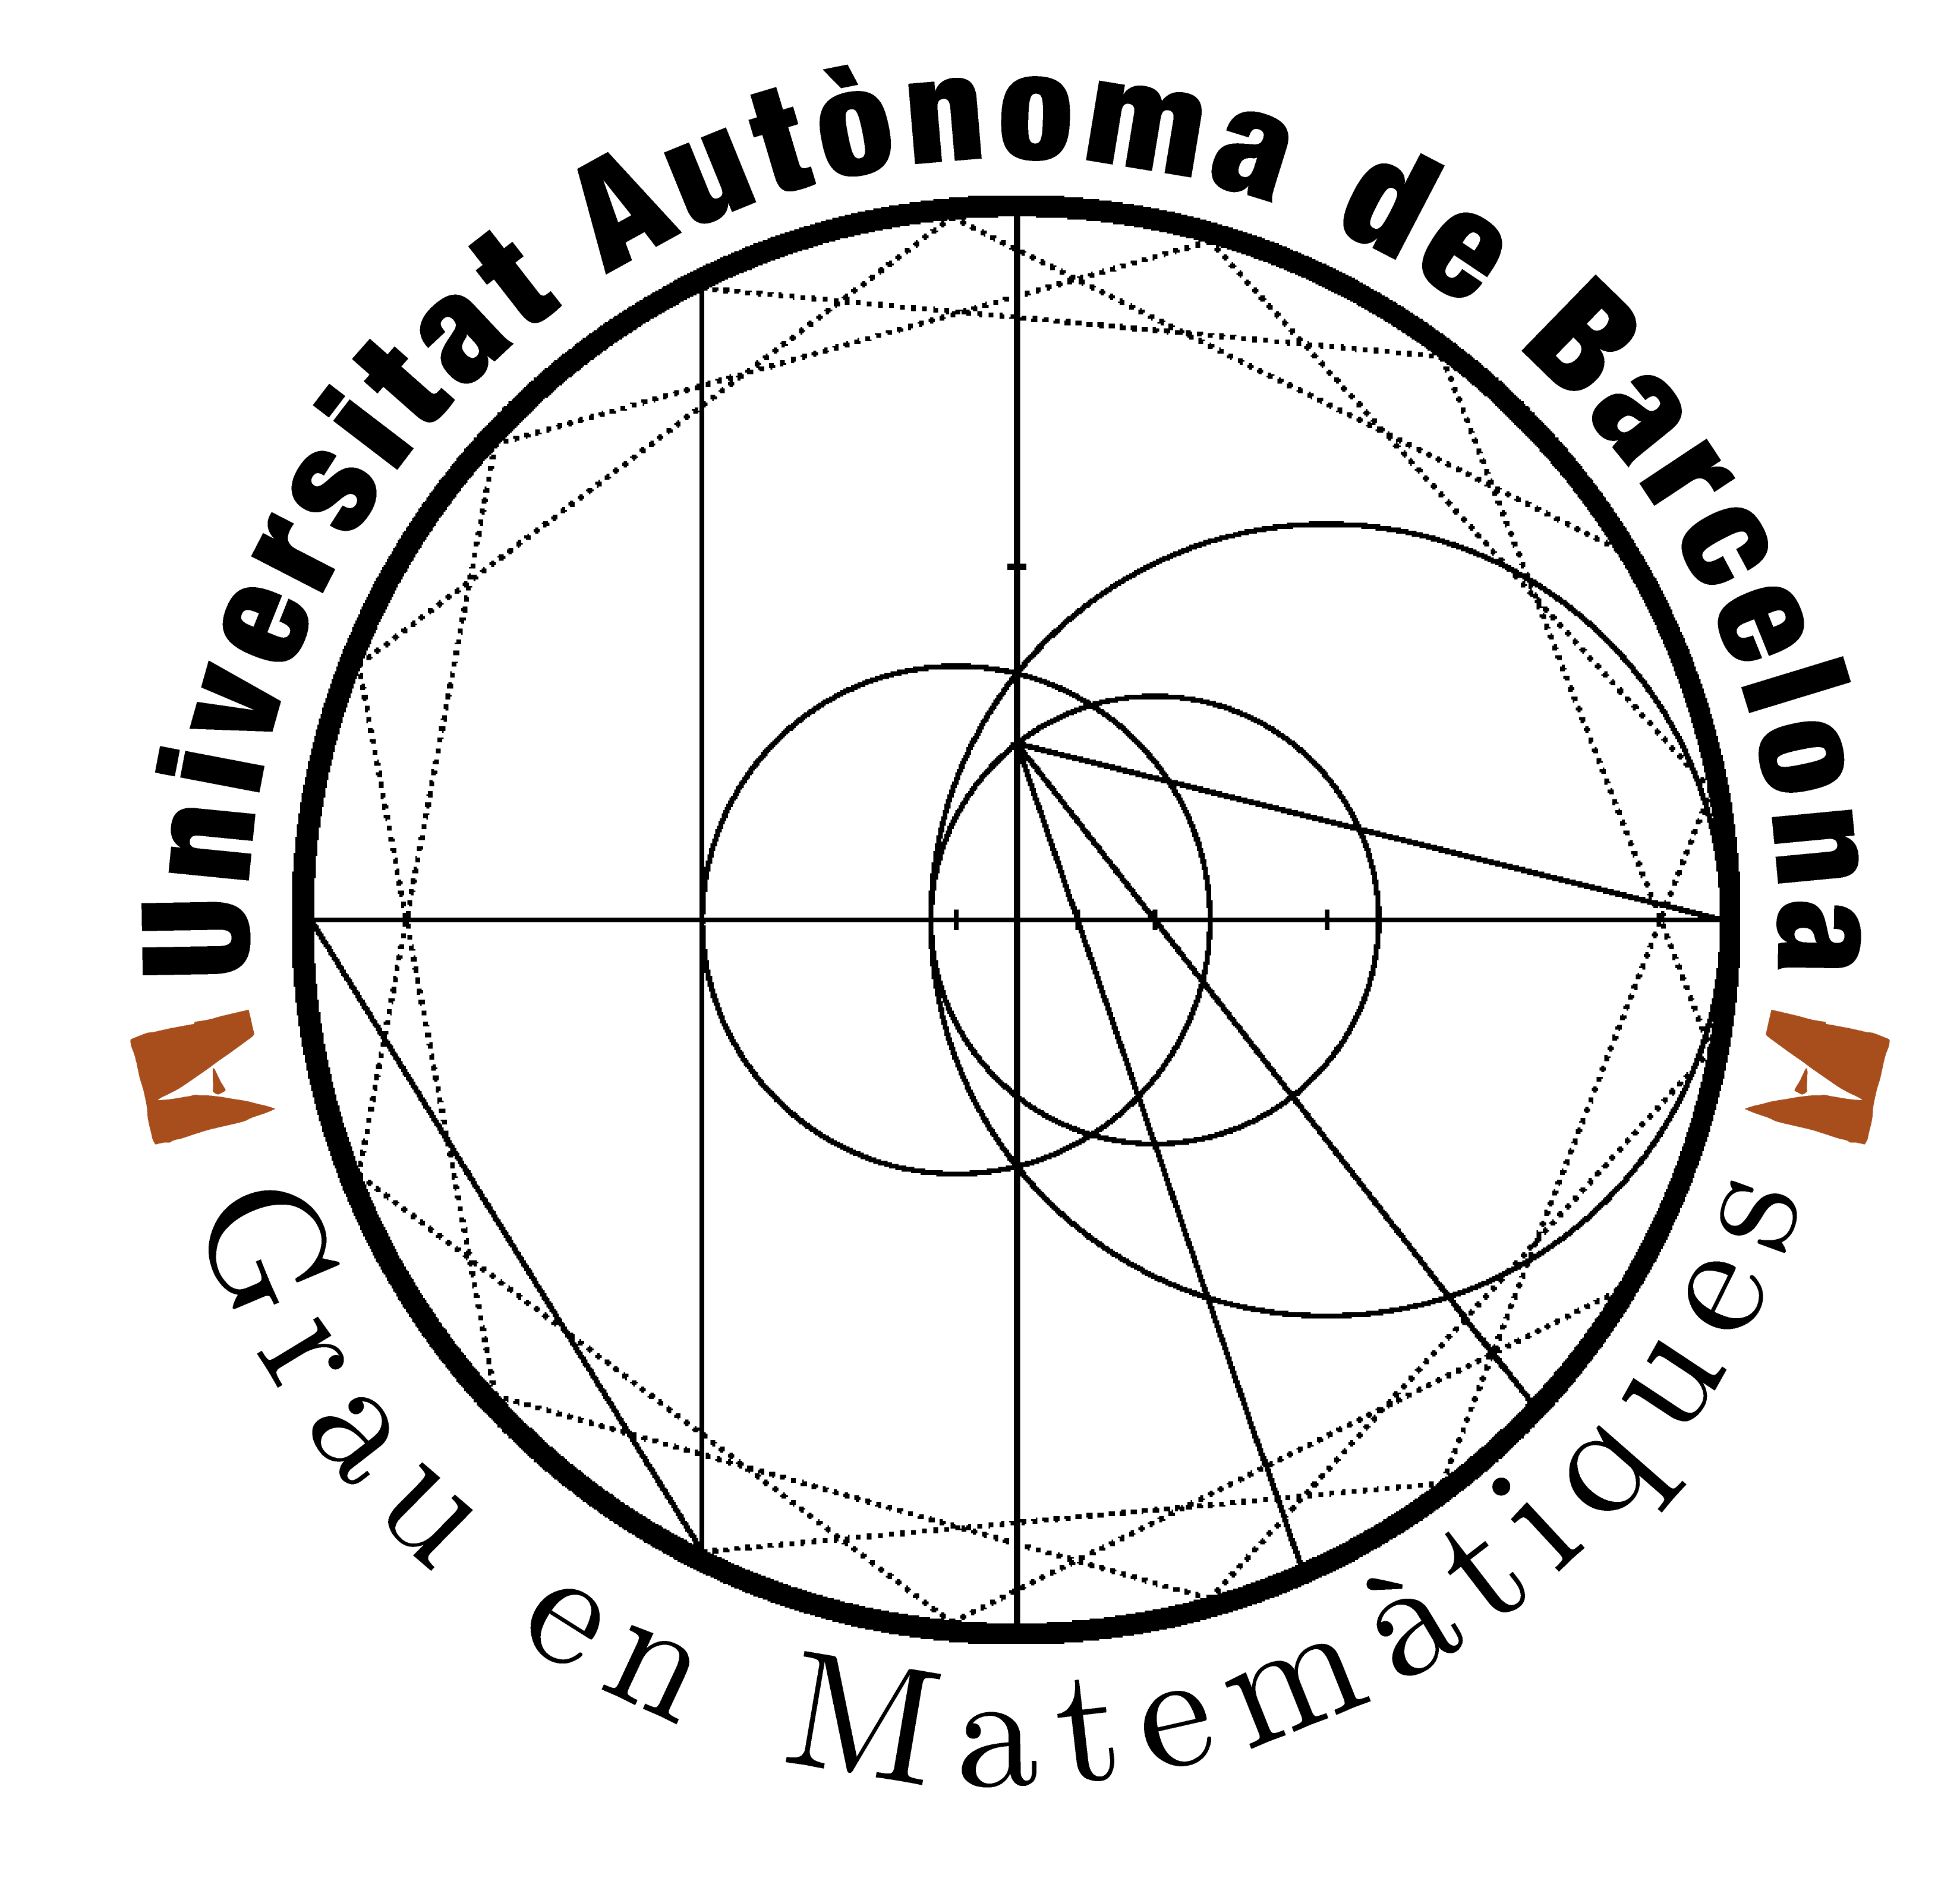
\includegraphics[width=0.75\textwidth]{Portada.png}\\\href{https://drive.google.com/open?id=1EgVV_YvOgo0p2FNcu4EG0DbQeUYI7Xt4}{Apunts de matemàtiques}}
\author{Claudi Lleyda Moltó}
\date{Les matemàtiques són un joc de definicions.}

\theoremstyle{plain}
\newtheorem{theorem}{Teorema}[subsection]
\newtheorem{proposition}[theorem]{Proposició}
\newtheorem{lemma}[theorem]{Lemma}
\newtheorem{corollary}[theorem]{Coro{\lgem}ari}
\newtheorem{note}[theorem]{Nota} %Amb la meva veu?
\newtheorem{observation}[theorem]{Observació} %Per reinterpretacions?
\newtheorem{example}[theorem]{Exemple}
\newtheorem{axiom}[theorem]{Axioma}

\theoremstyle{definition}
\newtheorem{definition}[theorem]{Definició}
\newtheorem{notation}[theorem]{Notació}

%\renewcommand{\sectionmark}[1]{\markright{#1}}

%\makeatletter\addto\captionscatalan{\renewcommand\partname{Assignatura}}\makeatother


\pagestyle{fancy}
\fancyhf{}
\rhead{\thepage}
\lhead{\rightmark}
\cfoot{}

\newenvironment{solution}{\renewcommand\qedsymbol{\(\lozenge\)}\renewcommand{\proofname}{Solució}\begin{proof}}{\end{proof}}

\DeclareMathOperator{\Long}{L}
\DeclareMathOperator{\Dist}{d}
\DeclareMathOperator{\B}{B}
\DeclareMathOperator{\R}{R}
\DeclareMathOperator{\omicron}{o}
\DeclareMathOperator{\Omicron}{O}
\DeclareMathOperator{\rang}{rang}
\DeclareMathOperator{\Ssup}{S}
\DeclareMathOperator{\sinf}{s}
\DeclareMathOperator{\Fr}{Fr}
\DeclareMathOperator{\St}{St}
\DeclareMathOperator{\mcd}{mcd}
\DeclareMathOperator{\mcm}{mcm}
\DeclareMathOperator{\ch}{ch}

\let\ker\relax
\DeclareMathOperator*{\ker}{ker}
\DeclareMathOperator*{\Ima}{Im}

%\setcounter{chapter}{-1}

%\makeatletter
%\def\thickhrulefill{\leavevmode \leaders \hrule height 1.2ex \hfill \kern \z@}
%\def\@makechapterhead#1{
%	\vspace*{10\p@}%
%	{\parindent \z@ \centering \reset@font
%		\thickhrulefill\quad
%		\scshape\bfseries\text{\@chapapp{} \hfill \thechapter}
%		\quad\thickhrulefill
%		\par\nobreak
%		\vspace*{10\p@}%
%		\interlinepenalty\@M
%		\hrule
%		\vspace*{10\p@}%
%		\Huge \bfseries #1 \par\nobreak
%		\par
%		\vspace*{10\p@}%
%		\hrule
%		\vspace*{15\p@}%
%	}}
%\makeatother

%\newcommand{\myref}[1]{\ref{#1}}
\newcommand{\myref}[1]{\mynameref{#1}{\csname r@#1\endcsname}}

\makeatletter
\def\mynameref#1#2{%
	\begingroup
	\edef\@mytxt{#2}%
	\edef\@mytst{\expandafter\@thirdoffive\@mytxt}%
	\ifx\@mytst\empty\ref{#1}\else
	\nameref{#1}\space\eqref{#1}\fi
	\endgroup
}
\makeatother

\makeatletter
\newcommand{\labelname}[1]{
	\def\@currentlabelname{#1}}
\makeatother

\begin{document}
	{\hypersetup{urlcolor=black,linkcolor=black}\maketitle\tableofcontents}
	\part{Introducció}
	\chapter{Coses per fer}
		Podeu trobar la versió actualitzada d'aquest pdf seguint aquest \href{https://drive.google.com/open?id=1EgVV_YvOgo0p2FNcu4EG0DbQeUYI7Xt4}{link}.
%	\subsection{Ignorar}
%	\begin{enumerate}
%		\item Definir \(\mathbb{R}^{+}\). (fot mandra)
%		\item Adjuntar documents: llegir i aplicar punt \textsl{1.8 Big Projects} de lshort.pdf.
%		\item Afegir més notes explicant la vida quan acabi. %sarcasm anyone?
%		\item Definir \(\omicron(\vec{h})\) (que tendeix a \(\vec{0}\)).
%		\item Definir imatge d'un conjunt per una funció (\(\Ima_{f}(U)\), \(f[U]\)...).
%		\item Definit obert, tancat, compacte...
%		\item Relacions d'equivalència.
%	\end{enumerate}
	\section{Àlgebra lineal}
	\subsection{Definicions}
	\begin{definition}[Forma bilineal definida estrictament positiva o negativa]
		\labelname{forma bilineal definida estrictament positiva o negativa}\label{def:bilineal definida estrictament positiva/negativa}
		Sigui \(M\) una forma bilineal simètrica. Preguntar a en Cedò.
	\end{definition}
	\begin{definition}[Norma d'una aplicació lineal]
		\labelname{norma d'una aplicació lineal}\label{def:Norma d'una aplicació lineal}
	\end{definition}
	\subsection{Proposicions}
	\begin{proposition}\label{prop:determinant diferent de zero linealment independents}
		Vectors linealment independents \(\Leftrightarrow\) determinant no nul.
	\end{proposition}
	\subsection{Teoremes}
	\begin{theorem}
		Sigui \(A=(a_{i,j})\in M_{n}(\mathbb{R})\) una matriu simètrica. Aleshores \(A\) és definida positiva si i només si
		\[\left|\begin{matrix}
		a_{1,1}&\cdots&a_{1,i}\\
		\vdots&&\vdots\\
		a_{i,1}&\cdots&a_{i,i}\\
		\end{matrix}\right|>0\]
		per a tot \(i\in\{1,\dots,n\}\).
		\begin{proof}
			Per inducció sobre \(n\).
		\end{proof}
	\end{theorem}
	\section{Funcions de variable real}
	\subsection{Definicions}
	\begin{definition}[Funció contínua]
		\labelname{funció contínua}\label{def:funcio continua}
		Sigui \(f\) una funció. Direm que \(f\) és contínua en \(a\) si
		\[\lim_{x\to a}f(x)=f(a).\]
	\end{definition}
	\begin{definition}[Partició, poligonal i longitud d'una poligonal]
		\labelname{partició}\label{def:partició}
		\labelname{poligonal}\label{def:poligonal}
		\labelname{longitud d'una poligonal}\label{def:longitud de poligonal}
		Sigui \((a,b)\) un interval de \(\mathbb{R}\). Direm que una partició de \((a,b)\) és un conjunt de escalars \(t_{0},\dots,t_{n}\in[a,b]\) que compleixen \(a=t_{0}<\dots<t_{n}=b\). Direm que \(t_{0},\dots,t_{n}\) són els nodes de la partició.
		
		Sigui \(f:(a,b)\to\mathbb{R}^{m}\) una funció. Definirem la poligonal \(P_{n}\) d'una partició en una funció \(f\) com
		\[P_{n}=f(t_{0}),\dots,f(t_{n}).\]
		Definim la longitud de la poligonal \(P_{n}\) com
		\[\Long(P_{n})=\sum_{i=0}^{n-1}\|f(t_{i+1})-f(t_{i})\|.\]
	\end{definition}
	\begin{definition}[Classe de diferenciabilitat d'una funció]
		\labelname{classe de diferenciabilitat d'una funció}\label{def:Classe de diferenciabilitat}
		Sigui \(f\) una funció \(n\)-vegades diferenciable amb \(f^{(n)}\) contínua. Direm que \(f\) és de classe \(\mathcal{C}^{n}\) o que \(f\in\mathcal{C}^{n}\).
	\end{definition}
	\begin{definition}[Funció monòtona]
		\labelname{funció monòtona}\label{def:funció monòtona}
		Sigui \(f:[a,b]\to\mathbb{R}\) una funció. Direm que és \(f\) és monòtona si, per a qualsevol \(x,y\in[a,b]\), \(x>y\) implica \(f(x)\geq f(y)\).
	\end{definition}
	\begin{definition}[Notació de Landau]
		\labelname{notació de Landau}\label{def:Landau}
		\(A(h)=\omicron(B(h))\dots\)
	\end{definition}
	\subsection{Proposicions}
	\begin{proposition}\label{prop:Derivable implica contínua}
		Siguin \(I\subseteq\mathbb{R}\) un interval i \(f:I\to\mathbb{R}\) una funció. Aleshores, si \(f\) és derivable en un punt \(a\in I\), \(f\) és contínua en \(a\).
	\end{proposition}
	\begin{proposition}
		Sigui \(f:[a,b]\to\mathbb{R}\) una funció acotada i monòtona. Aleshores \(f\) és integrable Riemann.
	\end{proposition}
	\subsection{Teoremes}
	\begin{theorem}[Equivalència entre normes]
		\labelname{Teorema de l'equivalència entre normes}\label{thm:Equivalència de normes}
		Si \(q(x)\) és una norma existeixen \(m,M\in\mathbb{R}^{+}\) tals que \(m\|x\|\leq q(x)\leq M\|x\|\) per a tot \(x\in\mathbb{R}^{m}\).
	\end{theorem}
	\begin{theorem}[Teorema del Valor Mig]
		\label{Teorema del Valor Mig}\label{thm:TVM}
		\emph{hmm trivial}
	\end{theorem}
	\begin{theorem}[Desigualtat de Cauchy-Schwarz]
		\labelname{Teorema de la Desigualtat de Cauchy-Schwarz}\label{thm:Desigualtat de C-S}
	\end{theorem}
	\begin{theorem}[Teorema de Taylor]
		\labelname{Teorema de Taylor}\label{thm:Teorema de Taylor} %caldrà adaptar-lo
		Sigui \((a,b)\subseteq\mathbb{R}\) un interval i \(f:(a,b)\to\mathbb{R}\) una funció de classe \(\mathcal{C}^{n}\). Aleshores, per a dos punts \(x,c\in(a,b)\), amb \(x<c\), existeix un punt \(x_{1}\in(x,c)\) tal que
		\[f(x)=f(c)+\sum_{k=1}^{n-1}\frac{f^{(k)}(c)}{k!}(x-c)^{k}+\frac{f^{(n)}(x_{1})}{n!}(x-c)^{n}.\]
	\end{theorem}
	\begin{theorem}[Teorema de Weierstrass]
		\labelname{Teorema de Weierstrass}\label{thm:Weierstrass màxims i mínims múltiples variables}
		Siguin \(U\subseteq\mathbb{R}^{d}\) un obert i \(f:U\to\mathbb{R}\) una funció. Aleshores, donat un compacte \(S\subset U\), si \(f\) és contínua en \(S\), \(f\) té un màxim i un mínim absoluts en \(S\).
	\end{theorem}
	\begin{theorem}[Teorema del sandvitx]
		\labelname{Teorema del sandvitx}\label{thm:sandvitx}
	\end{theorem}
	\begin{theorem}[Teorema de Rolle]
		\labelname{Teorema de Rolle}\label{thm:Teorema de Rolle}
		Sigui \(f:[a,b]\subset\mathbb{R}\longrightarrow\mathbb{R}\) una funció derivable en \((a,b)\) tal que \(f(a)=f(b)\). Aleshores existeix un cert \(c\in(a,b)\) tal que \(f'(c)=0\).
	\end{theorem}
	\section{Trobar lloc per tot això}
	\begin{definition}[Conjunt obert, tancat...]
		\labelname{conjunt obert}\label{def:obert}
		\labelname{conjunt tancat}\label{def:tancat}\label{conjunt obert, tancat...}\label{todo:conjunt definit per desigualtats estrictes és compacte}
		\end{definition}
	\begin{definition}[Relació d'equivalència]
		\labelname{relació d'equivalència}\label{def:relació d'equivalència}
		\end{definition}
	\begin{definition}[Continuïtat uniforme]
		\labelname{continuïtat uniforme}\label{def:uniformement contínua}
		Siguin \(U\subseteq\mathbb{R}^{d},V\subseteq\mathbb{R}^{m}\) dos oberts i \(f:U\to V\) una funció. Aleshores direm que \(f\) és uniformement contínua en un conjunt \(S\subseteq U\) si per a tot \(\varepsilon>0\) existeix un \(\delta>0\) tals que
		\[d_{U}(x,y)<\varepsilon\text{ i }d_{V}(f(x)-f(y))<\delta\]
		per a tot punt \(x,y\in U\).
	\end{definition}
	\begin{theorem}[Teorema de Heine]
		\labelname{Teorema de Heine}\label{thm:Teorema de Heine}
		Siguin \(U\subseteq\mathbb{R}^{d}\) dos oberts, \(S\subset U\) un compacte i \(f:U\to\mathbb{R}^{m}\) una funció contínua. Aleshores \(f\) és uniformement contínua en \(S\). %pàg 91 de Mathematical Analysis d'en Apostol (55 del pdf)
	\end{theorem}
	\begin{definition}[Funció indicatriu]
		\labelname{funció indicatriu}\label{def:funció indicatriu}
		Siguin \(X\) un conjunt i \(A\subseteq X\) un subconjunt de \(X\). Definim la funció indicatriu de \(A\) com una funció
		\[1_{A}:X\longrightarrow\{0,1\}\]
		tal que
		\begin{displaymath}
		1_{A}(x)=\begin{cases}
		1 & x\in A \\
		0 & x\notin A.
		\end{cases}
		\end{displaymath}
	\end{definition}
	\begin{theorem}[Teorema de la divisió Euclidiana]
		\labelname{Teorema de la divisió Euclidiana}\label{thm:divisió euclidiana}
	\end{theorem}
	\part{Càlcul en diverses variables i optimització}
	\chapter{Càlcul diferencial}
	\section{Introducció}
	\subsection{Arcs en múltiples variables}
	\begin{definition}[Arcs a l'espai]
		\labelname{arc}\label{def:arc}
		\labelname{arc continu}\label{def:arc continu}
		\labelname{arc simple}\label{def:arc simple}
		\labelname{arc tancat}\label{def:arc tancat}
		\labelname{arc regular}\label{def:arc regular}
		\labelname{arc de classe $\mathcal{C}^{n}$}\label{def:arc de classe de diferenciabilitat n}
		Siguin \((a,b)\subseteq\mathbb{R}\) un interval, \(f:(a,b)\to\mathbb{R}^{m}\) una funció i \(\Gamma\) el conjunt definit per
		\[\Gamma=\left\{x\in\mathbb{R}^{m}:x=f(t)\text{ per a tot }t\in(a,b)\right\},\]
		aleshores direm que \(\Gamma\) és un arc a \(\mathbb{R}^{m}\). També direm que \(f\) defineix o recorre aquest arc.
		Així mateix donem les següents definicions:
		\begin{enumerate}
			\item Direm que \(\Gamma\) és un arc continu si \(f\) és contínua en \((a,b)\).
			\item Direm que \(\Gamma\) és un arc simple si \(f\) és injectiva en \((a,b)\).
			\item Si \(f\) està definida en \([a,b]\) direm que \(f\) va de \(f(a)\) a \(f(b)\) o que \(f(a)\) n'és el punt inicial i \(f(b)\) el punt final. Si \(f(a)=f(b)\) direm que \(\Gamma\) és un arc tancat.
			\item Direm que \(\Gamma\) és un arc regular si \(f\) és derivable en \((a,b)\).
			\item Direm que \(\Gamma\) és un arc de classe \(\mathcal{C}^{n}\) si \(f^{(n)}\) existeix i és contínua en \((a,b)\).
		\end{enumerate}
	\end{definition}
	\begin{definition}[Longitud d'un arc continu]
		\labelname{longitud d'un arc continu}\label{def:long recorregut arc continu}
		Sigui \(\Gamma\) un arc continu i \(f\) una manera de recórrer \(\Gamma\) donada per
		\[f:(a,b)\subseteq\mathbb{R}\longrightarrow\mathbb{R}^{m}\]
		Amb \(m\in\mathbb{N}\), \(m>1\).
		
		Considerem la partició \(a=t_{0}<\dots<t_{n}=b\). Observem que els punts donats per \(f(t_{i})\) per a tot \(i\in\{0,\dots,n\}\) determinen una poligonal, \(P_{n}\), la longitud de la qual és, per la definició de \myref{def:longitud de poligonal}
		\[\Long(P_{n})=\sum_{i=0}^{n-1}\|f(t_{i+1})-f(t_{i})\|.\]
		Aleshores definim la longitud de \(f\) com
		\[\Long(f)=\lim_{n\to\infty}\Long(P_{n}).\]
		Direm que els arcs amb recorreguts de longitud finita són arcs rectificables.
	\end{definition}
	\begin{proposition}
		Sigui \(\Gamma\) un arc de classe \(\mathcal{C}^{1}\). Aleshores \(\Gamma\) és rectificable.
		\begin{proof}
			Sigui \(f\) una funció que recorre \(\Gamma\) tal que
			\begin{align*}
			f:(a,b)\subseteq\mathbb{R}&\longrightarrow\mathbb{R}^{m}\\
			t&\longmapsto(x_{1}(t),\dots,x_{m}(t)).
			\end{align*}
			
			Donada una partició de \((a,b)\), \(a=t_{0}<\dots<t_{n}=b\) que defineix una poligonal \(P_{n}=f(t_{0}),\dots,f(t_{n})\). Aleshores la longitud de la poligonal  és, per la definició de \myref{def:partició},
			\[\Long(P_n)=\sum_{i=0}^{n-1}\|f(t_{i+1})-f(t_{i})\|=\sum_{i=0}^{n-1}\sqrt{\sum_{j=1}^{m}\left(x_{j}(t_{i+1})-x_{j}(t_{i}))\right)^{2}}.\]
			
			Per la proposició \myref{prop:Derivable implica contínua} \(f\) és contínua en \((a,b)\), i per tant pel \myref{thm:TVM} tenim
			\[x_{j}(t_{i+1})-x_{j}(t_{i})=x_{j}'(\xi_{ij})(t_{i+1}-t_{i}),\]
			amb \(t_{i}<\xi_{ij}<t_{i+1}\), per a tot \(i\in\{0,\dots,n-1\},\ j\in\{1,\dots,m\}\). Per tant
			\begin{equation}\label{eq:1}
			\Long(P_{n})=\sum_{i=0}^{n-1}(t_{i+1}-t_{i})\sqrt{\sum_{j=1}^{m}\left(x_{j}'(\xi_{ij})\right)^2}.
			\end{equation}
			
			Ara volem veure que \(\xi_{ij}=\xi_{i}\) quan \(n\) tendeix a infinit. Observem que
			\[\lim_{n\to\infty}t_{i}=\lim_{n\to\infty}t_{i+1}.\]
			
			I com que \(t_{i}<\xi_{ij}<t_{i+1}\) tenim que \(\xi_{ij}=\xi_{i}\) per a tot \(j\in\{1,\dots,m\}\). Així veiem que si \(n\to\infty\) podem reescriure \eqref{eq:1} com
			\begin{displaymath}
			\Long(P_{n})=\sum_{i=0}^{n-1}(t_{i+1}-t_{i})\|f'(\xi_{i})\|=\int_{a}^{b}\|f'(t)\|dt.
			\end{displaymath}
			
			I ja hem acabat. Com que \(f\in\mathcal{C}^{1}\) tenim \(f'\) contínua, i \(a,b\in\mathbb{R}\), aquesta integral és finita i \(\Gamma\) és rectificable, com volíem veure.
		\end{proof}
	\end{proposition}
	\subsection{Oberts connexos}
	\begin{definition}[Conjunt arc-connex o connex]
		\labelname{conjunt arc-connex}\label{def:Arc-connex}
		\labelname{conjunt connex}\label{def:connex}
		Sigui \(U\subseteq\mathbb{R}^{d}\) un obert. Direm que \(U\) és arc-connex si donats dos punts \(P,Q\in U\) existeix una funció \(f\) que defineix un arc continu tal que \(f:[a,b]\longrightarrow U\) amb \(P=f(a),\ Q=f(b)\).
		Direm que \(U\) és connex si el segment que els uneix està tot dins \(U\).
	\end{definition}
	\begin{proposition}Sigui \(U\subseteq\mathbb{R}^{d}\) un obert. Donats dos arc-connexos \(U_{1}, U_{2}\subseteq U\) amb \(U_{1}\cup U_{2}=U\), si \(U_{1}\cap U_{2}\neq\emptyset\Longrightarrow U\) és arc-connex.
		\begin{proof}
			Siguin \(P,Q\) dos punts en \(U\) tals que \(P\in U_{2}^{\complement}\) i \(Q\in U_{1}^{\complement}\), i \(R\in U_{1}\cap U_{2}\) un altre punt. Com que \(U_{1}\) i \(U_{2}\) són arc-connexos, per la definició de \myref{def:Arc-connex} existeixen dos arcs continus \(f,g\) tals que
			\begin{displaymath}
			f:[a,b]\longrightarrow U_{1},\quad
			g:[b,c]\longrightarrow U_{2},
			\end{displaymath}
			on \(f(a)=P\), \(f(b)=g(b)=R\) i \(g(c)=Q\).
			Aleshores definim la funció
			\[h(t)=
			\begin{cases}
			f(t) & \text{si }a\leq t\leq b\\
			g(t) & \text{si }b<t\leq b.
			\end{cases}\]
			
			Tenim que \(h\) defineix un arc continu en \(U\), i per la definició de \myref{def:long recorregut arc continu}, \(U\) és arc-connex.
		\end{proof}
	\end{proposition}
	\begin{definition}[Distància en un arc-connex]
		\labelname{distància en un arc-connex}\label{def:distància en un arc-connex}
		Sigui \(U\subseteq\mathbb{R}^{d}\) un arc-connex, siguin \(P,Q\in U\) i \(F\) el conjunt de totes les funcions \(f\) que defineixen un arc continu en \(U\) amb \(f(a)=P\), \(f(b)=Q\). Definim la distància entre \(P\) i \(Q\) en \(U\) com
		\begin{displaymath}
		\Dist_{U}(P,Q)=\inf_{f\in F}\Long(f).
		\end{displaymath}
	\end{definition}
	\begin{observation}\label{obs:connex metrica}
		Notem que si \(U\) és connex \(\Dist_{U}(P,Q)=\|P-Q\|\).
	\end{observation}
	\begin{proposition}
		Siguin \(U\subseteq\mathbb{R}^{d}\) un arc-connex i \(P,Q,R\in U\) tres punts. Aleshores
		\begin{enumerate}
			\item\label{enumerate:distancies en arc-connexos 1} \(\Dist_{U}(P,Q)=\Dist_{U}(Q,P)\geq0\)
			\item\label{enumerate:distancies en arc-connexos 2} \(\Dist_{U}(P,Q)=0\Longleftrightarrow P=Q\)
			\item\label{enumerate:distancies en arc-connexos 3} \(\Dist_{U}(P,Q)\leq \Dist_{U}(P,R)+\Dist_{U}(R,Q)\) (desigualtat triangular) %aconseguir que aquesta merda vagi al final de la línia
		\end{enumerate}
		\begin{proof}
			Sigui \(f:[a,b]\to U\) una funció contínua amb \(f(a)=P\) i \(f(b)=Q\), i  amb \(\Long(f)=\inf_{f\in F}\Long(f)\), on \(F\) és el conjunt de funcions contínues de \([a,b]\) en \(U\) que van de \(P\) a \(Q\). %revisar
			
			 Per veure el punt \eqref{enumerate:distancies en arc-connexos 1} fem
			\begin{align*}
			\Dist_{U}(P,Q)&=\inf_{f\in F}\Long(f)\\
			&=\inf_{f\in F}\lim_{n\to\infty}\left(\sum_{i=0}^{n-1}(t_{i+1}-t_{i})\sqrt{\sum_{j=1}^{d}\left(x_{j}'(\xi_{ij})\right)^2}\right)\\
			&=\inf_{f\in F}\lim_{n\to\infty}\left(\sum_{i=0}^{n-1}(-1)(t_{n-(i+1)}-t_{n-i})\sqrt{\sum_{j=1}^{d}\left(x_{j}'(\xi_{ij})\right)^2}\right)\\
			&=\inf_{f\in F}(-1)\lim_{n\to\infty}\left(\sum_{i=0}^{n-1}(t_{n-(i+1)}-t_{n-i})\sqrt{\sum_{j=1}^{d}\left(x_{j}'(\xi_{ij})\right)^2}\right)\\
			&=\inf_{f\in F}(-1)\int_{a}^{b}\|f'(t)\|dt\\
			&=\inf_{f\in F}\int_{b}^{a}\|f'(t)\|dt=\inf_{f\in F}\Long(f)=\Dist_{U}(Q,P)\geq0.
			\end{align*}
			
			Continuem veient el punt \eqref{enumerate:distancies en arc-connexos 2}. Suposem \(P=Q\) i considerem, amb \(\varepsilon>0\), la bola oberta \(\B(\varepsilon,P)\subset U\). Aquesta bola és connexa i, pel coro{\lgem}ari \myref{obs:connex metrica}, \(\Dist_{U}(P,Q)=\|P-Q\|=0\Longleftrightarrow P=Q\).%refer salts de línia potser
			
			Acabem veient el punt \eqref{enumerate:distancies en arc-connexos 3}. Sigui \(F_{1}\) el conjunt de funcions contínues en \(U\) que van de \(P\) a \(R\) i \(F_{2}\) el conjunt de funcions contínues en \(U\) que van de \(R\) a \(Q\). Aleshores
				\begin{displaymath}
				\Dist_{U}(P,Q)=\inf_{f\in F}\Long(f)\leq\inf\left(\inf_{F_{1}}\Long(g)+\inf_{F_{2}}\Long(h)\right)=\Dist_{U}(P,R)+\Dist_{U}(R,Q).
				\end{displaymath}%revisar el 3 fort. Segurament fer per contradicció i ínfims.
			Observem que aquestes són les mateixes propietats de una distància.
		\end{proof}
	\end{proposition}
	\section{Funcions diferenciables}
	\subsection{Diferencial d'una funció en múltiples variables}
	\begin{definition}[Derivada direccional]
		\labelname{derivada direccional}\label{def:derivada direccional}
		Sigui \(U\subseteq\mathbb{R}^{d}\) un obert, \(t\in\mathbb{R}\) un escalar, \(a\in U\) un punt, \(\vec{u}\) un vector de \(\mathbb{R}^{d}\) i \(f\) una funció definida per
		\begin{align*}
		f:U&\longrightarrow\mathbb{R}^{m}\\
		a&\longmapsto(f_{1}(a),\dots,f_{m}(a)),
		\end{align*}
		i considerem, per a tot \(i\in\{1,\dots,m\}\), els límits
		\[D_{\vec{u}}f_{i}(a)=\lim_{t\to0}\frac{f_{i}(a+t\vec{u})-f_{i}(a)}{t}.\]
		Si tots aquests límits existeixen, direm que la derivada de \(f\) en direcció \(\vec{u}\) és
		\[D_{\vec{u}}f(a)=\left(D_{\vec{u}}f_{1}(a),\dots,D_{\vec{u}}f_{m}(a)\right).\]
		
		Si \(\vec{u}\) és l'\(i\)-èsim vector de la base canònica utilitzarem la notació \(D_{i}f(a)\).
	\end{definition}
	\begin{proposition}\label{prop:derivades direccionals lineals pel producte d'escalars}
		Siguin \(U\subseteq\mathbb{R}^{d}\) un obert, \(f:U\to\mathbb{R}^{m}\) una funció, \(D_{\vec{u}}f(a)\) la seva derivada direccional respecte el vector \(\vec{u}\) de \(\mathbb{R}^d\) i \(\lambda\in\mathbb{R}\) un escalar. Aleshores
		\[D_{\lambda\vec{u}}f(a)=\lambda D_{\vec{u}}f(a).\]
		\begin{proof}
			Tenim que, per a tot \(i\in \{1,\dots,m\}\),
			\begin{align*}
			D_{\lambda\vec{u}}f_{i}(a)&=\lim_{t\to0}\frac{f_{i}(a+\lambda t\vec{u})-f_{i}(a)}{t}\\
			&=\lim_{t\to0}\lambda\frac{f_{i}(a+\lambda t\vec{u})-f_{i}(a)}{\lambda t}\\
			&=\lambda\lim_{t\to0}\frac{f_{i}(a+\lambda t\vec{u})-f_{i}(a)}{\lambda t}=\lambda D_{\vec{u}}f_{i}(a).\qedhere
			\end{align*}
		\end{proof}
	\end{proposition}
	\begin{definition}[Diferencial d'una funció]
		\labelname{diferencial d'una funció}\label{def:diferencial}
		Siguin \(U\subseteq\mathbb{R}^{d}\) un obert i \(f:U\to\mathbb{R}^{m}\) una funció i \(a\in U\) un punt. Direm que el diferencial de \(f\) en \(a\) és una aplicació lineal \(df(a):U\to\mathbb{R}^{m}\) tal que, donat un vector \(\vec{h}\) de \(\mathbb{R}^{d}\)
		\[f(a+\vec{h})=f(a)+df(a)(\vec{h})+\omicron(\vec{h}),\quad \|\vec{h}\|\to0.\]
		Direm que \(f\) és diferenciable en \(a\) si existeix aquest \(df(a)\).
	\end{definition}
	\begin{observation}
		Observem que en aquesta definició, si \(d=1\), \(f\) és diferenciable en \(a\) \(\Longleftrightarrow f\) és derivable en \(a\), i \(df(a)(\vec{h})=\vec{h}f'(a)\) (Si \(d=1\), multiplicar per un vector de \(\mathbb{R}\) és com multiplicar per un escalar).
	\end{observation}
	\begin{proposition}\label{prop:Diferenciable implica contínua}
		Siguin \(U\subseteq\mathbb{R}^{d}\) un obert i \(f:U\to\mathbb{R}^{m}\) una funció diferenciable en un punt \(a\in U\). Aleshores \(f\) és contínua en \(a\).
		\begin{proof}
			Sigui \(df(a)\) el diferencial de \(f\) en \(a\). Per la definició de \myref{def:diferencial} tenim que, per a qualsevol vector \(\vec{h}\) de \(\mathbb{R}^d\)
			\[f(a+\vec{h})=f(a)+df(a)(\vec{h})+\omicron(\vec{h}),\quad \|\vec{h}\|\to0.\]
			Com que \(df(a)\) és lineal, \(df(a)(\vec{h})\to(0,\dots,0)\Leftrightarrow\|\vec{h}\|\to0\). Així veiem que
			\[\lim_{\|\vec{h}\|\to0}f(a+\vec{h})-f(a)-df(a)(\vec{h})=\omicron(\vec{h}).\]
			I això compleix la definició de \myref{def:funcio continua}, per tant \(f\) és contínua en el punt \(a\).
		\end{proof}
	\end{proposition}
	\begin{proposition}\label{prop:diferenciable iff components diferenciables}
		Siguin \(U\subseteq\mathbb{R}^{d}\) un obert, \(a\in U\) un punt i \(f\) una funció tal que
		\begin{align*}
		f:U&\longrightarrow\mathbb{R}^{m}\\
		a&\longmapsto(f_{1}(a),\dots,f_{m}(a)).
		\end{align*}
		Aleshores
		\[f\text{ és diferenciable en }a\Leftrightarrow f_{i}\text{ és diferenciable en a }\forall i\in \{1,\dots,m\}.\]
		\begin{proof}
			Per la definició de \myref{def:diferencial} tenim que, per a qualsevol vector \(\vec{h}\) de \(\mathbb{R}^d\)
			\[f(a+\vec{h})=f(a)+df(a)(\vec{h})+\omicron(\vec{h}),\quad \|\vec{h}\|\to0.\]
			El que és equivalent a
			\[\lim_{\|\vec{h}\|\to0}\frac{f(a+\vec{h})-f(a)-df(a)(\vec{h})}{\|\vec{h}\|}=0.\]
			Sabent que \(f(a)=(f_{1}(a),\dots,f_{m}(a))\) podem entendre aquest límit com el següent, amb un vector al numerador, que descomponem com:
			\[\lim_{\|\vec{h}\|\to0}\frac{(f_{1}(a+\vec{h})-f_{1}(a)-df_{1}(a)(\vec{h}),\dots,f_{m}(a+\vec{h})-f_{m}(a)-df_{m}(a)(\vec{h}))}{\|\vec{h}\|}=0,\]
			si i només si%límits respecten continuïtat
			\[\lim_{\|\vec{h}\|\to0}\frac{f_{i}(a+\vec{h})-f_{i}(a)-df_{i}(a)(\vec{h})}{\|\vec{h}\|}=0\]
			per a tot \(i\in\{1,\dots,m\}\).
			
			Tenint en compte la definició de \myref{def:diferencial}, és equivalent a dir que, per a tot \(i\in\{1,\dots,m\}\), \(f_{i}\) és diferenciable en el punt \(a\).
			%Cal remarcar que podem fer això ja que \(f\) i \(f_{1},\dots,f_{m}\) (depenent del costat de la implicació) són contínues, per la proposició \myref{prop:Diferenciable implica contínua}.%revisar (potser no cal), buscar manera de marcar la línia llarga de la proof per fer-ne referència i dir a algun lloc que els límits "respecten" la continuïtat.
		\end{proof}
	\end{proposition}
	\begin{proposition}\label{prop:derivades parcials i diferencial}
		Siguin \(U\subseteq\mathbb{R}^{d}\) un obert i \(f:U\to\mathbb{R}^{m}\) una funció diferenciable en un punt \(a\in U\). Aleshores tenim que
		\begin{enumerate}
			\item Donat un vector \(\vec{u}\) de \(\mathbb{R}^d\), \(D_{\vec{u}}f(a)\) existeix i \(df(a)(\vec{u})=D_{\vec{u}}f(a)\).
			\item El diferencial de \(f\) en \(a\), \(df(a)\), és únic.
		\end{enumerate}
		\begin{proof}
			Sigui \(\vec{u}\) un vector de \(\mathbb{R}^d\). Tenim que, si \(\lambda\in\mathbb{R}\), \(\lambda\neq0\)
			\[f(a+\lambda\vec{u})=f(a)+df(a)(\lambda\vec{u})+\omicron(\lambda\vec{u})\]
			\[f(a+\lambda\vec{u})-f(a)=\lambda df(a)(\vec{u})+\omicron(\lambda\vec{u})\]
			\[\frac{f(a+\lambda\vec{u})-f(a)}{\lambda}=df(a)(\vec{u})+\frac{\omicron(\lambda\vec{u})}{\lambda}\]
			Per tant, amb \(\lambda\to0\), per la definició de \myref{def:derivada direccional} tenim
			\[D_{\vec{u}}f(a)=df(a)(\vec{u}).\]
			Amb aquesta demostració també es veu la unicitat del diferencial d'una funció en un punt. %xd revisar. Però crec que està bé.
		\end{proof}
	\end{proposition}
	\begin{observation}\label{obs:derivades direccionals lineals}
		Com a conseqüència del primer apartat veiem que si \(f\) és diferenciable en \(a\) existeixen totes les seves derivades direccionals i que aquestes compleixen que, donats dos vectors \(\vec{u},\vec{v}\) i dos escalars \(\lambda,\mu\), \(D_{\lambda\vec{u}+\mu\vec{v}}f(a)=\lambda D_{\vec{u}}f(a)+\mu D_{\vec{v}}(a)\).
	\end{observation}
	\begin{theorem}[Condició suficient per a la diferenciabilitat]
		\labelname{Teorema d'una condició suficient per a la diferenciabilitat}\label{thm:Condició suficient per diferenciable}
		Siguin \(U\subseteq\mathbb{R}^{d}\) un obert, \(f:U\to\mathbb{R}^{m}\) una funció, \(a\in U\) un punt i \(\B(a,\varepsilon)\), una bola centrada en \(a\) de radi \(\varepsilon>0\). Si les derivades direccionals de \(f\), \(D_{i}f(x)\), existeixen per a tot punt \(x\in\B(a,\varepsilon)\), per a tot \( i\in\{1,\dots,d\}\) i són contínues en \(a\), aleshores \(f\) és diferenciable en \(a\).
		\begin{proof}
			Donat un vector \(\vec{h}\) de \(\mathbb{R}^{d}\), considerem la diferencia
			\[f(a+\vec{h})-f(a),\]
			amb \(a=(a_{1},\dots,a_{d})\) i \(\vec{h}=(h_{1},\dots,h_{d})=\sum_{i=1}^{d}h_{i}\vec{e}_{i}\), on \(\vec{e_{i}}\) és l'\(i\)-èsim vector de la base canònica, i denotarem \(\vec{h}_{n}=\sum_{i=1}^{n}h_{i}\vec{e}_{i}\) per a \(1\leq n\leq d\) i \(\vec{h}_{0}=(0,\dots,0)\). Escrivim la suma telescòpica
			\begin{equation}\label{eq:thm:Condició suficient per diferenciable 1}
			f(a+\vec{h})-f(a)=\sum_{i=1}^{d}\left(f(a+\vec{h}_{i})-f(a+\vec{h}_{i-1})\right).
			\end{equation}
			
			El primer terme d'aquesta suma telescòpica és \(f(a+h_{1}\vec{e}_{1})-f(a)\), i per la definició de \myref{def:derivada direccional} això és
			\[f(a+h_{1}\vec{e}_{1})-f(a)=h_{1}D_{1}f(a)+h_{1}\omicron(\vec{h}),\]
			i la resta de termes de \eqref{eq:thm:Condició suficient per diferenciable 1} són
			\[f(a+\vec{h}_{k-1}+h_{k}\vec{e}_{k})-f(a+\vec{h}_{k-1}).\]
			Veiem que aquestes expressions varien només en \(h_{k}\vec{e}_{k}\), que correspon a la \(k\)-èsima component, i com que les derivades parcials de \(f\) existeixen, això vol dir que aquestes expressions són contínues, per tant podem aplicar el \myref{thm:TVM} per a funcions d'una variable i tenim que, per a tot \(2\leq k\leq d\) existeix un escalar \(\xi_{k}\) tal que
			\[f(a+\vec{h}_{k-1}+h_{k}\vec{e}_{k})-f(a+\vec{h}_{k-1})=h_{k}D_{k}f(\xi_{k})\]
			on \(\xi_{k}\) està al segment que uneix \(a+\vec{h}_{k-1}+h_{k}\vec{e}_{k}\) i \(a+\vec{h}_{k-1}\).
			
			Ara notem que quan \(\vec{h}\to0\) tindrem \(a+\vec{h}_{k-1}+h_{k}\vec{e}_{k}\to a\) i com que, per hipòtesi, les derivades direccionals són contínues
			\[h_{k}D_{k}f(\xi_{k})=h_{k}D_{k}f(a)+h_{k}\omicron(\vec{h})\]
			i obtenim
			\begin{align*}
			f(a+\vec{h})-f(a)&=\sum_{i=1}^{d}h_{i}D_{i}f(a)+\sum_{i=1}^{d}h_{i}\omicron(\vec{h})\\
			&=\sum_{i=1}^{d}D_{h_{i}\vec{e}_{i}}f(a)+\sum_{i=1}^{d}h_{i}\omicron(\vec{h})
			\end{align*}
			i mentre \(a+\vec{h}\in\B(a,\varepsilon)\), el que tenim satisfà la definició de \myref{def:diferencial} per la proposició \myref{prop:derivades parcials i diferencial}, i per tant \(f\) és diferenciable en \(a\).
		\end{proof}
	\end{theorem}
	\begin{note}
		Notem que en aquesta demostració només hem hagut d'utilitzar la continuïtat de \(d-1\) de les derivades parcials de \(f\) en \(a\). per tant en veritat tenim prou amb veure que totes les derivades parcials de \(f\) existeixen en \(a\) i que almenys totes menys una d'aquestes són contínues en \(a\) per poder dir que \(f\) és diferenciable en \(a\), però a aquest curs només es dona l'enunciat reduït.
	\end{note}
	\begin{proposition}
		Siguin \(U\subseteq\mathbb{R}^{d}\) un obert i \(f,g:U\to\mathbb{R}^{m}\) dues funcions diferenciables en un punt \(a\in U\) amb diferencials \(df(a),dg(a)\), respectivament. Aleshores \(f+g\) és diferenciable en \(a\) i té per diferencial \(df(a)+dg(a)\).
		\begin{proof}
			Siguin \(\vec{u}\) un vector de \(\mathbb{R}^{d}\) i \(D_{\vec{u}}f(a),\ D_{\vec{u}}g(a)\) les derivades parcials de \(f\) i \(g\), respectivament, en el punt \(a\) amb direcció \(\vec{u}\). La derivada parcial de \(f+g\) en \(a\) amb direcció \(\vec{u}\) és \(D_{\vec{u}}(f+g)(a)\). Com que les derivades direccionals es comporten, per definició, com les derivades d'una variable, tenim
			\[D_{\vec{u}}f(a)+D_{\vec{u}}g(a)=D_{\vec{u}}(f+g)(a),\]
			i per la proposició \myref{prop:derivades parcials i diferencial}, com que l'argument no depèn de \(\vec{u}\), ja hem acabat.
		\end{proof}
	\end{proposition}
	\subsection{La Matriu Jacobiana i la regla de la cadena}
	\begin{definition}[Matriu Jacobiana]
		\labelname{matriu Jacobiana}\label{def:Jacobiana}
		Siguin \(U\subseteq\mathbb{R}^{d}\) un obert i \(f:U\to\mathbb{R}^{m}\) una funció diferenciable en un punt \(a\in U\). Aleshores definim la matriu Jacobiana de \(f\) en \(a\) com
		\[\left[\begin{matrix}
		D_{1}f_{1}(a) & D_{2}f_{1}(a) & \cdots & D_{d}f_{1}(a)\\
		D_{1}f_{2}(a) & D_{2}f_{2}(a) & \cdots & D_{d}f_{2}(a)\\
		\vdots & \vdots && \vdots \\
		D_{1}f_{m}(a) & D_{2}f_{m}(a) & \cdots & D_{d}f_{m}(a)
		\end{matrix}\right].\]
	\end{definition}
	\begin{proposition}\label{prop:justificació Jacobiana}
		Siguin \(U\subseteq\mathbb{R}^{d}\) un obert, \(f:U\to\mathbb{R}^{m}\) una funció diferenciable en un punt \(a\in U\), \(df(a)\) el diferencial de \(f\) en el punt \(a\) i \(\vec{h}=(h_{1},\dots,h_{d})\) un vector de \(\mathbb{R}^{d}\). Aleshores
		\[df(a)(\vec{h})=
		\left[\begin{matrix}
		D_{1}f_{1}(a) & \cdots & D_{d}f_{1}(a)\\
		\vdots && \vdots \\
		D_{1}f_{m}(a) & \cdots & D_{d}f_{m}(a)
		\end{matrix}\right]
		\left[\begin{matrix}
		h_{1}\\
		\vdots\\
		h_{d}
		\end{matrix}\right],\]
		és a dir, la matriu Jacobiana de \(f\) en \(a\) és la matriu associada del diferencial de \(f\) en el punt \(a\).
		\begin{proof}
			Observem que aquest enunciat té sentit per la definició de \myref{def:diferencial} i la definició de \myref{def:Jacobiana}.
			
			Donada la base canònica de \(\mathbb{R}^{d}\), \((\vec{e_{1}},\dots,\vec{e_{d}})\), tenim
			\[df(a)(\vec{h})=\sum_{i=1}^{d}h_{i}df(a)(\vec{e_{i}})=\sum_{i=1}^{d}h_{i}D_{i}f(a),\]
			i si \(f(a)=(f_{1}(a),\dots,f_{m}(a))\),
			\begin{equation}\label{eq:2}
			D_{i}f(a)=
			\left[\begin{matrix}
			D_{i}f_{1}(a)\\
			\vdots\\
			D_{i}f_{m}(a)
			\end{matrix}\right].
			\end{equation}
			Per tant, podem reescriure aquestes dues igualtats com
			\[df(a)(\vec{h})=
			\left[\begin{matrix}
			D_{1}f(a)~\cdots~D_{d}f(a)
			\end{matrix}\right]
			\left[\begin{matrix}
			h_{1}\\\vdots\\h_{d}
			\end{matrix}
			\right].\]
			On, recordant \eqref{eq:2},
			\[\left[\begin{matrix}
			D_{1}f(a)~\cdots~D_{d}f(a)
			\end{matrix}\right]=
			\left[\begin{matrix}
			D_{1}f_{1}(a) & D_{2}f_{1}(a) & \cdots & D_{d}f_{1}(a)\\
			D_{1}f_{2}(a) & D_{2}f_{2}(a) & \cdots & D_{d}f_{2}(a)\\
			\vdots & \vdots && \vdots \\
			D_{1}f_{m}(a) & D_{2}f_{m}(a) & \cdots & D_{d}f_{m}(a)
			\end{matrix}\right].\]
			Així que
			\[df(a)(\vec{h})=
			\left[\begin{matrix}
			D_{1}f_{1}(a) & D_{2}f_{1}(a) & \cdots & D_{d}f_{1}(a)\\
			D_{1}f_{2}(a) & D_{2}f_{2}(a) & \cdots & D_{d}f_{2}(a)\\
			\vdots & \vdots && \vdots \\
			D_{1}f_{m}(a) & D_{2}f_{m}(a) & \cdots & D_{d}f_{m}(a)
			\end{matrix}\right]
			\left[\begin{matrix}
			h_{1}\\h_{2}\\\vdots\\h_{d}
			\end{matrix}
			\right].\]
			Així veiem que la matriu Jacobiana de \(f\) en \(a\) està ben definida com a matriu associada del diferencial de \(f\) en \(a\).
		\end{proof}
	\end{proposition}
	\begin{observation}\label{obs:diferencial defineix espai tangent}
		Suposem \(m=1\). Recordant la definició de \myref{def:diferencial} i denotant \(x=a+\vec{h}\), \(a=(a_{1},\dots,a_{d}),\ x=(x_{1},\dots,x_{d})\)
		\[f(x)-f(a)-\omicron(\|x-a\|)=df(a)(x-a)\]
		i per la definició de \myref{def:Jacobiana} tenim
		\[f(x)-f(a)-\omicron(\|x-a\|)=
		\left[\begin{matrix}
		D_{1}f(a)~\cdots~D_{d}f(a)
		\end{matrix}\right]
		\left[\begin{matrix}
		x_{1}-a_{1}\\
		\vdots\\
		x_{d}-a_{d}
		\end{matrix}\right].\]
		El que, quan \(\vec{h}\to0\), ens diu que és una aproximació a
		\[(x_{1}-a_{1})D_{1}f(a)+\dots+(x_{d}-a_{d})D_{d}f(a)=f(x)-f(a),\]
		el que és un espai afí de dimensió \(d+1\) tangent a \(f\) en el punt \(a\).
	\end{observation}
	\begin{theorem}[Regla de la cadena]
		\labelname{Teorema de la regla de la cadena}\label{thm:regla de la cadena}
		Siguin \(U\subseteq\mathbb{R}^{d}\) un obert i \(f:U\to\mathbb{R}^{m}\) una funció diferenciable en un punt \(a\in U\) i siguin \(V\subseteq\mathbb{R}^{m}\) un obert i \(g:V\to\mathbb{R}^{p}\) una funció diferenciable en un punt \(f(a)=b\in V\). Aleshores \(g(f(x))\) és diferenciable en \(a\) amb diferencial \(dg(b)(df(a)(\vec{h}))\), on \(df(a)\) i \(dg(b)\) són els diferencials de \(f\) i \(g\) en \(a\) i \(b\), respectivament, i \(\vec{h}\) és un vector de \(\mathbb{R^{d}}\).
		\begin{proof}
			Per la definició de \myref{def:diferencial}, tenim
			\[f(a+\vec{h})=f(a)+df(a)(\vec{h})+\omicron(\vec{h}),\quad \|\vec{h}\|\to0.\]
			Reescrivim amb \(x=a+\vec{h}\) i \(y=b+\vec{h}\)
			\[f(x)=f(a)+df(a)(x-a)+\omicron(x-a),\]
			\[g(y)=g(b)+dg(b)(y-b)+\omicron(y-b).\]
			Si fem \(y=f(x)\) i substituïm en la segona equació obtenim
			\[g(f(x))=g(b)+dg(b)(f(a)+df(a)(x-a)+\omicron(x-a)-b)+\omicron(f(x)-b)\]
			Si simplifiquem i utilitzem la linealitat del diferencial obtenim
			\[g(f(x))=g(b)+dg(b)(df(x-a))+dg(b)(\omicron(x-a))+\omicron(f(x)-b)\]
			Ara només hem de veure que \(dg(b)(\omicron(x-a))\) i \(\omicron(f(x)-b)\) són \(\omicron(x-a)\). El primer el podem veure amb que
			\[\|dg(b)(\omicron(x-a))\|\leq\|dg(b)\|\omicron(\|x-a\|).\] % fer: explicar
			I com que quan \(x\to a,\ f(a)\to b\) (donat per \(\vec{h}\to0\)), ja que \(f\) és contínua. Aleshores podem escriure
			\[f(x)-b=df(a)(x-a)+\omicron(x-a),\]
			i  observant el cas \(x\to a\) trobem que \(\|f(x)-b\|\leq C\|x-a\|\), on \(C\in\mathbb{R}\) és la norma de l'aplicació lineal \(dg(b)\). % referència
		\end{proof}
	\end{theorem}
	\subsection{Gradient, punts crítics i extrems relatius}
	\begin{definition}[Funció escalar]
		\labelname{funció escalar}\label{def:funció escalar}
		Sigui \(U\subseteq\mathbb{R}^{d}\) un obert i \(f:U\to\mathbb{R}\) una funció. Direm que \(f\) és una funció escalar de \(d\) variables si \(f\) és diferenciable per a tot \(x\in U\).%revisar
	\end{definition}
	\begin{definition}[Conjunts de nivell]
		\labelname{conjunts de nivell}\label{def:conjunts de nivell}
		Siguin \(U\subseteq\mathbb{R}^{d}\) un obert i \(f:U\to\mathbb{R}\) una funció. Aleshores direm que, per a tot \(C\in\mathbb{R}\),
		\[L_{C}=\{x\in U:f(x)=C\}\]
		és el conjunt de nivell \(C\) de la funció \(f\).
	\end{definition}
	\begin{definition}[Gradient d'una funció]
		\labelname{gradient d'una funció}\label{def:gradient}
		Siguin \(U\subseteq\mathbb{R}^{d}\) un obert i \(f:U\to\mathbb{R}\) una funció escalar. Definim el gradient de \(f\) en un punt \(a\in U\) com el vector
		\[\nabla f(a)=(D_{1}f(a),\dots,D_{d}f(a)).\]
	\end{definition}
	\begin{proposition}
		Siguin \(U\subseteq\mathbb{R}^{d}\) un obert, \(f:U\to\mathbb{R}\) una funció escalar i \(\vec{u}=(u_{1},\dots,u_{d}\) un vector de \(\mathbb{R}^{d}\). Aleshores
		\[\langle\nabla f(a),\vec{u}\rangle=D_{\vec{u}}f(a).\]
		\begin{proof}
			Ho veiem per la definició de \myref{def:gradient}, la definició de \myref{def:derivada direccional} i l'observació \myref{obs:derivades direccionals lineals}. Tenim
			\begin{align*}
			\langle\nabla f(a),\vec{u}\rangle&=u_{1}D_{1}f(a)+\dots+u_{d}D_{d}f(a)\tag{\myref{def:gradient}}\\
			&=D_{u_{1}\vec{e}_{1}}f(a)+\dots+D_{u_{d}\vec{e}_{1}}f(a)\tag{\myref{def:derivada direccional}}\\
			&=D_{u_{1}\vec{e}_{1}+\dots+u_{d}\vec{e}_{1}}f(a)\tag{Observació \myref{obs:derivades direccionals lineals}}\\
			&=D_{\vec{u}}f(a),
			\end{align*}
			com volíem demostrar.
		\end{proof}
	\end{proposition}
	\begin{observation}\label{obs:gradient ortogonal}
	El gradient d'una funció en un punt és perpendicular al conjunt de nivell que conté el punt.%revisar una mica
	\end{observation}
	\begin{proposition}
		Sigui \(U\subseteq\mathbb{R}^{d}\) un obert, \(f:U\to\mathbb{R}\) una funció escalar i \(D_{\vec{u}}f(a)\) la derivada direccional de \(f\) en la direcció \(\vec{u}\), on \(\vec{u}\) és un vector de \(\mathbb{R}^{d}\). Aleshores \(D_{\vec{u}}f(a)\) és màxim \(\Longleftrightarrow\ \vec{u}=\lambda\nabla f(a)\), amb \(\lambda\in\mathbb{R}\).
		\begin{proof}
			Pel \myref{thm:Desigualtat de C-S} tenim, amb \(\|\vec{u}\|=1\)
			\[-\|\nabla f(a)\|\leq\|\langle\nabla f(a),\vec{u}\rangle\|\leq\|\nabla f(a)\|\]
			\[-\|\nabla f(a)\|\leq\|D_{\vec{u}}(a)\|\leq\|\nabla f(a)\|,\]
			però si prenem \(\vec{u}=\frac{\nabla f(a)}{\|\nabla f(a)\|}\) tenim \(D_{\vec{u}}f(a)=\nabla f(a)\). Amb això es veu que el gradient d'una funció en un punt ens dona la direcció de màxim creixement de la funció en el punt.
		\end{proof}
	\end{proposition}
	\begin{observation}
		Veiem que, donat que \(\nabla f(a)\) ens diu la direcció de màxim creixement de \(f\) en el punt \(a\), \(-\nabla f(a)\) ens dirà la direcció de màxim decreixement de \(f\) en \(a\).
	\end{observation}
	\begin{definition}[Extrems relatius i punts crítics]
		\labelname{extrem relatiu}\label{def:extrems relatius}
		\labelname{punt crític}\label{punts crítics}
		Sigui \(U\subseteq\mathbb{R}^{d}\) un obert, \(a\in U\) un punt i \(f:U\to\mathbb{R}\) una funció escalar. Direm que el punt \(a\) és un extrem relatiu de \(f\) si hi ha una bola de radi \(r>0\) centrada en el punt \(a\), \(\B(a,r)\), tal que, per a tot \(x\in\B(a,r)\), \(f(a)\geq f(x)\) (direm que \(a\) és un màxim relatiu) o tal que \(f(a)\leq f(x)\) (direm que \(a\) és un mínim relatiu).
		
		Si \(f(a)\geq f(x)\) o \(f(a)\leq f(x)\), per a tot \(x\in U\), direm que \(a\) és un màxim o un mínim absolut de \(f\) en \(U\), respectivament.
		
		També direm que \(a\) és un punt crític si \(\nabla f(a)=\vec{0}\).
	\end{definition}
	\begin{proposition}\label{prop:Identificació d'extrems relatius}
		Sigui \(U\subseteq\mathbb{R}^{d}\) un obert i \(f:U\to\mathbb{R}\) una funció escalar diferenciable en \(a\). Aleshores
		\[a\text{ és un màxim o un mínim relatiu de }f\Longrightarrow \nabla f(a)=\vec{0}.\]
		\begin{proof}
			Si \(\vec{u}\) és un vector qualsevol de \(\mathbb{R}^{d}\), la funció \(f(a+t\vec{u})\), amb \(t\in\mathbb{R}\) té un extrem relatiu en \(t=0\), i per tant la seva derivada ha de ser 0; \(D_{\vec{u}}f(a)=0\), i com això no depèn de \(\vec{u}\), per la definició de \myref{def:gradient}, \(D_{\vec{u}}=\langle\nabla f(a),\vec{u}\rangle=0\), el que és equivalent a \(\nabla f(a)=\vec{0}\).
		\end{proof}
	\end{proposition}
	\begin{observation}\label{obs:extrem relatiu és punt crític}
		Amb la definició de \myref{def:extrems relatius} i la proposició \myref{prop:Identificació d'extrems relatius} tenim que el punt \(a\) és un màxim o mínim relatiu de \(f\) si \(a\) és un punt crític de \(f\).
	\end{observation}
	\begin{definition}[Punt de sella d'una funció]
		\labelname{punt de sella d'una funció}\label{def:punt de sella}
		Sigui \(f\) una funció i \(a\) un punt del seu domini. Si \(a\) és un punt crític però no és ni màxim ni mínim local direm que \(a\) és un punt de sella de \(f\).
		
		Observem que aquesta definició té sentit per l'observació \myref{obs:extrem relatiu és punt crític}.
	\end{definition}
	\subsection{Canvis de coordenades diferenciables}
	\begin{definition}[Homeomorfisme i difeomorfisme]
		\labelname{homeomorfisme}\label{def:homeomorfisme}
		\labelname{difeomorfisme}\label{def:difeomorfisme}
		Siguin \(U,V\subseteq\mathbb{R}^{d}\) dos oberts i \(\Phi:U\longleftrightarrow V\) una aplicació bijectiva tal que \(\Phi,\Phi^{-1}\) siguin contínues. Aleshores direm que \(\Phi\) és un homeomorfisme. Si pensem \(\Phi\) com
		\begin{align*}
		\Phi:U&\longleftrightarrow V\\
		a&\longmapsto(v_{1}(a),\dots,v_{d}(a))
		\end{align*}
		aleshores donat un punt \(a\in U\), interpretem \(v_{1}(a),\dots,v_{d}(a)\) com les noves coordenades del punt \(a\). Amb aquest nou sistema els punts que fan d'eixos de coordenades, que són les famílies de punts definits per
		\[\{x\in U:v_{i}(x)=v_{j}(a)\Leftrightarrow i\neq j,\forall i,j\in\{1,\dots,d\}\},\]
		que són tots els punts amb totes les coordenades iguals, excepte la \(j\)-èsima.
		
		Si \(\Phi,\Phi^{-1}\) són diferenciables direm que és un canvi de coordenades diferenciable o que és un difeomorfisme.
	\end{definition}
	\begin{proposition}\label{prop:difeomorfisme diferenciable invertible}
		Siguin \(U,V\subseteq\mathbb{R}^{d}\) dos oberts i \(\Phi:U\longleftrightarrow V\) un difeomorfisme. Aleshores
		\[d(\Phi^{-1})=(d\Phi)^{-1}.\]
		\begin{proof}
			Sabem que \(\Phi^{-1}\) existeix i és diferenciable per la definició de \myref{def:difeomorfisme}; direm que \(\Phi\) és diferenciable en un punt \(a\), amb diferencial \(d\Phi(a)\) i \(\Phi^{-1}\) és diferenciable en un punt \(b=\Phi(a)\), amb diferencial \(d\Phi^{-1}(a)\). Volem veure que \(d(\Phi^{-1})=(d\Phi)^{-1}\).
			
			Considerem la funció \(\Phi^{-1}(\Phi)\) i un vector \(\vec{h}\) de \(\mathbb{R}^{d}\) fixe. Aleshores el seu diferencial en \(a\) aplicat a \(\vec{h}\) és, pel \myref{thm:regla de la cadena}
			\[Id_{U}(a)=d((\Phi^{-1}(\Phi))(a))(\vec{h})=d((\Phi^{-1})(b))(d\Phi(a)(\vec{h}))\]
			i
			\[Id_{V}(b)=d(\Phi((\Phi^{-1}))(b))(\vec{h})=d(\Phi(a))(d\Phi^{-1}(b)(\vec{h}))\]
			Amb això tenim que \(d(\Phi^{-1})\) també és la inversa de \(d\Phi\) pels dos costats, i per tant \(d(\Phi^{-1})=(d\Phi)^{-1}\), com volíem demostrar.
		\end{proof}%REVISAR MOLT https://math.stackexchange.com/questions/207392/invertible-derivative
	\end{proposition}
	\begin{corollary}\label{corollary:difeomorfime determinant}
		Donada una funció \(\Phi\) un difeomorfisme diferenciable en un punt \(a\). Aleshores
		\[\det(df(a))\neq0.\]
	\end{corollary}
	\begin{definition}[Derivades parcials d'una funció]
		\labelname{derivades parcials d'una funció}\label{def:Derivades parcials}
		Siguin \(U\subseteq\mathbb{R}^{d}\) un obert, \(a=(a_{1},\dots,a_{d})\) un punt de \(U\) i \(f\) una funció definida per
		\begin{align*}
		f:U&\longrightarrow\mathbb{R}^{m}\\
		a&\longmapsto(f_{1}(a),\dots,f_{m}(a)).
		\end{align*}
		Aleshores, donat un \(t\in\mathbb{R}\), direm que la derivada parcial de \(f\) respecte la seva \(i\)-èsima coordenada és
		\[\frac{\partial f}{\partial x_{i}}(a)=\lim_{t\to0}\frac{f(a_{1},\dots,a_{i}+t,\dots,a_{d})-f(a)}{t}.\]
		Notem que això és equivalent a derivar respecte la \(i\)-èsima variable prenent les altres variables com a constants.
	\end{definition}
	\begin{proposition}
		Siguin \(U,V\subset\mathbb{R}^{d}\) dos oberts i \(\Phi:U\to V\) un difeomorfisme tal que donat un punt \(a\in U\), \(\Phi(a)=(\Phi_{1}(a),\dots,\Phi_{d}(a))=(v_{1},\dots,v_{d})\). Aleshores, donada una funció \(f:U\to V\),\[\frac{\partial f}{\partial v_{i}}=\sum_{j=1}^{d}\frac{\partial f}{\partial x_{j}}\frac{\partial x_{j}}{\partial v_{i}}.\]		
		\begin{proof}
			%TODO
		\end{proof}
	\end{proposition}
	%FER per regla de la cadena i després demostrar la mítica 2.7.2
	\section{Teoremes de la funció implícita i inversa}
	\subsection{Dependència i independència funcional}
	\begin{definition}[Dependència funcional]
		\labelname{dependència funcional}\label{def:dependència funcional}
		Siguin \(U\subseteq\mathbb{R}^{d}\) un obert i \(f:U\to\mathbb{R}^{m}\) una funció. Donades \(v_{1},\dots,v_{k}:U\to\mathbb{R}\) \(k\) funcions, direm que \(f\) depèn funcionalment de \(v_{1},\dots,v_{k}\) si existeix una funció \(h:\mathbb{R}^{k}\to\mathbb{R}^{m}\) tal que
		\[f(x)=h(v_{1}(x),\dots,v_{k}(x)),\ \forall x\in U.\]
	\end{definition}
	\begin{proposition}\label{prop:dependència funcional 4 punts}
		Siguin \(U\subseteq\mathbb{R}^{d}\) un obert, \(f:U\to\mathbb{R}^{m}\) una funció i \(v_{1},\dots,v_{d}\), \(d\) funcions escalars sobre \(U\) que defineixen un sistema de coordenades que anomenarem \(\Phi(x)=(v_{1}(x),\dots,v_{d}(x))\). Aleshores, donat un \(k<d\) els següents enunciats són equivalents:
		\begin{enumerate}
			\item\label{enumerate:dependència funcional 4 punts 1} \(f\) depèn funcionalment de \(v_{1},\dots,v_{k}\) per a tot \(x\in U\).
			\item\label{enumerate:dependència funcional 4 punts 2} \(\nabla f(x)\) és combinació lineal de \(\nabla v_{1}(x),\dots,\nabla v_{k}(x)\) per a tot \(x\in U\).
			\item\label{enumerate:dependència funcional 4 punts 3} La matriu que té per files \(\nabla v_{1}(x),\dots,\nabla v_{k}(x)\) i \(\nabla f(x)\) té rang \(k\) per a tot \(x\in U\).
			\item\label{enumerate:dependència funcional 4 punts 4} \(\frac{\partial f}{\partial v_{k+1}}=\dots=\frac{\partial f}{\partial v_{d}}=0\)
		\end{enumerate}
%		\begin{proof}
%			fer
%		\end{proof}
%		\textbf{Ignorar aquesta demostració per ara}
%		\begin{proof}
%			Tenim que \eqref{enumerate:dependència funcional 4 punts 2}\(\Leftrightarrow\)\eqref{enumerate:dependència funcional 4 punts 3} és clar ja que es tracta d'àlgebra lineal.
%			
%			Comencem veient \eqref{enumerate:dependència funcional 4 punts 1}\(\Rightarrow\)\eqref{enumerate:dependència funcional 4 punts 2}. Suposem que \(f\) depèn funcionalment de les \(v_{1},\dots,v_{k}\). Aleshores existeix una funció \(h\) tal que per a tot \(x\in U\), \(f(x)=h(v_{1}(x),\dots,v_{k}(x))\). Pel \myref{thm:regla de la cadena} tenim, per a tot \(i\in\{1,\dots,d\}\),
%			\[\frac{\partial f}{\partial x_{i}}=\sum_{j=1}^{k}\frac{\partial h}{\partial y_{j}}\frac{\partial y_{j}}{\partial x_{i}},\]
%			on \(y_{j}\) es refereix a la \(j\)-èsima coordenada en \(h\).
%			
%			D'aquí deduïm que
%			\[\nabla f(x)=\frac{\partial h}{\partial y_{1}}(v_{1}(x),\dots,v_{k}(x))\nabla v_{1}(x)+\dots+\frac{\partial h}{\partial y_{k}}(v_{1}(x),\dots,v_{k}(x))\nabla v_{k}(x),\]
%			i tenim \((\mathit{1}\Rightarrow\mathit{2})\).
%			
%			Ara veiem \((\mathit{2}\Rightarrow\mathit{4})\). Com que, per hipòtesi, les funcions \(v_{1},\dots,v_{d}\) defineixen un sistema de coordenades, en aquest nou sistema de coordenades \(\frac{\partial f}{\partial v_{i}}\) quantifica la variació de \(f\) respecte la \(i\)-èsim eix, però com que tenim que \(\nabla f(x)\) és combinació lineal de \(\nabla v_{1}(x),\dots,\nabla v_{k}(x)\) per a tot \(x\in U\), la variació de \(f\) en les noves coordenades queda determinada per les primeres \(k\) funcions del sistema de coordenades donat per \(\Phi\), per tant tenim \(\frac{\partial f}{\partial v_{k+1}}=\dots=\frac{\partial f}{\partial v_{d}}=0\).
%			
%			Ara només ens queda demostrar que \((\mathit{4}\Rightarrow\mathit{1})\). Com que \(\Phi\) és un difeomorfisme i per tant bijectiva (per la definició de \myref{def:difeomorfisme}) considerem la seva inversa, \(\Phi^{-1}(y)=(u_{1}(y),\dots,u_{d}(y))\) i prenem
%			\[f(\Phi^{-1}(y))=f(u_{1}(y),\dots,u_{d}(y))\]
%			
%			Per tant, tenim \(\mathit{2}\Rightarrow\mathit{4}\Rightarrow\mathit{1}\Rightarrow\mathit{2}\Leftrightarrow\mathit{3}\) i hem acabat.
%		\end{proof}
%		\begin{proof}
%			Comencem veient \((\mathit{1}\Rightarrow\mathit{2})\).
%			
%			Suposem que \(f\) depèn funcionalment de les \(v_{1},\dots,v_{k}\). Aleshores existeix una funció \(h\) tal que per a tot \(x\in U\), \(f(x)=h(v_{1}(x),\dots,v_{k}(x))\). Pel \myref{thm:regla de la cadena} tenim, per a tot \(i\in\{1,\dots,d\}\)
%			\[\frac{\partial f}{\partial x_{i}}=\sum_{j=1}^{k}\frac{\partial h}{\partial y_{j}}\frac{\partial y_{j}}{\partial x_{i}},\]
%			on \(y_{j}\) es refereix a la \(j\)-èsima coordenada en \(h\).
%			
%			D'aquí deduïm que
%			\[\nabla f(x)=\frac{\partial h}{\partial y_{1}}(v_{1}(x),\dots,v_{k}(x))\nabla v_{1}(x)+\dots+\frac{\partial h}{\partial y_{k}}(v_{1}(x),\dots,v_{k}(x))\nabla v_{k}(x),\]
%			i tenim \((\mathit{1}\Rightarrow\mathit{2})\).
%			
%			Per veure \((\mathit{1}\Leftarrow\mathit{2})\) en tindrem prou amb demostrar que \((\mathit{1}\Leftrightarrow\mathit{4})\), ja que es tractarà d'un cas particular.
%			
%			Per veure \((\mathit{1}\Leftrightarrow\mathit{4})\) observem que, ja que \(\Phi\) correspon a un sistema de coordenades, tenim que el diferencial de \(\Phi\), \(d\Phi\) existeix i és invertible (per la definició de \myref{def:difeomorfisme} i proposició \myref{prop:difeomorfisme diferenciable invertible}). Per tant, vist que \(d\Phi\) és invertible, la seva \myref{def:Jacobiana} té determinant diferent de 0 (pel coro{\lgem}ari \myref{corollary:difeomorfime determinant}) per a tot \(x\in U\). Per tant, \(\nabla v_{1}(x),\dots,\nabla v_{k}(x)\) són linealment independents per a tot \(x\in U\), i tenim que \(v_{1}(x),\dots,v_{k}(x)\) són funcionalment independents per a tot \(x\in U\) (a partir dels punts \eqref{enumerate:dependència funcional 4 punts 1} i \eqref{enumerate:dependència funcional 4 punts 2} d'aquesta mateixa proposició, que ja hem demostrat). %mirar de no repetir-me tant
%			
%			Fixant-nos en que \(\Phi\) és un nou sistema de coordenades, tenim que derivar respecte a \(v_{i}\) és equivalent a buscar la derivada parcial respecte la \(i\)-èsima coordenada en el nou sistema de coordenades. Per tant, com vam veure a la justificació de la definició de \myref{def:Jacobiana}, tenim
%			\[df=\frac{\partial f}{\partial v_{1}}dv_{1}+\dots+\frac{\partial f}{\partial v_{d}}dv_{d},\]
%			però com que \(\nabla f(x)\) és combinació lineal de \(\nabla v_{1}(x),\dots,\nabla v_{k}(x)\) per a tot \(x\in U\), ha de ser
%			\[\frac{\partial f}{\partial v_{k+1}}=\dots=\frac{\partial f}{\partial v_{d}}=0.\]
%			
%			I per acabar, vist que es tracta de dependència lineal és obvi que \((\mathit{2}\Leftrightarrow\mathit{3})\).
%		\end{proof}
	\end{proposition}
	\begin{theorem}\label{thm:sistema de coordenades en un entorn iff gradients linealment independents}
		Siguin \(U\subseteq\mathbb{R}^{d}\) un obert i \(v_{1},\dots,v_{k}\in\mathcal{C}^{1}\) \(k<d\) funcions escalars definides en \(U\). Aleshores, donat un punt \(a\in U\) i un real \(\varepsilon>0\), les funcions \(v_{1},\dots,v_{k}\) formen un sistema de coordenades en \(\B(\varepsilon,a)\subset U\) si i només si els seus gradients en \(a\), \(\nabla v_{1}(a),\dots,\nabla v_{k}(a)\), són linealment independents.
		\begin{proof}
			Siguin \(U\subseteq\mathbb{R}^{d}\) un obert i \(v_{1},\dots,v_{k}\in\mathcal{C}^{1}\) \(k\) funcions escalars definides en \(U\) que formen un sistema de coordenades en \(\B(\varepsilon,a)\subset U\). Considerem les \(d-k\) funcions escalars definides en \(U\) \(v_{k+1},\dots,v_{d}\) tal que \(v_{1},\dots,v_{d}\) formin un sistema de coordenades de \(U\). Per la proposició \myref{prop:dependència funcional 4 punts} tenim que aquestes \(d\) funcions són funcionalment independents, el que ens diu que el determinant de la matriu composta per els seus gradients en un punt \(x\), \(\nabla v_{1}(x),\dots,\nabla v_{d}(x)\) té determinant no nul per a tot \(x\in U\). Per tant, tenim que \(\nabla v_{1}(x),\dots,\nabla v_{d}(x)\) són linealment independents per a tot \(x\in U\) i, en particular, que \(\nabla v_{1}(a),\dots,\nabla v_{k}(a)\) són linealment independents. %revisar maomeno
		\end{proof}
	\end{theorem}
	\subsection{Varietats}
	\begin{definition}[Varietat]
		\labelname{varietat}\label{def:varietat}
		Siguin, amb \(m<d\), \(U\subseteq\mathbb{R}^{m},\ S\subseteq\mathbb{R}^{d}\) dos oberts, \(M\subseteq\mathbb{R}^{d}\) un conjunt i \(r>0\) un radi. Aleshores, si per a tot punt \(p\in M\), existeix un homeomorfisme \(H:U\to S\cap\B(p,r)\) direm que \(M\) és una varietat de dimensió \(m\) de \(\mathbb{R}^{d}\).
	\end{definition} %nota explicant que parametritza que
	\begin{definition}[Varietat regular]
		\labelname{varietat regular}\label{def:varietat regular o diferenciable}
		Siguin, amb \(m<d\), \(U\subseteq\mathbb{R}^{m},\ S\subseteq\mathbb{R}^{d}\) dos oberts amb \((0,\dots,0)=0\in U\). Aleshores, donat un conjunt \(M\subseteq\mathbb{R}^{d}\), direm que \(M\) és una varietat regular de dimensió \(m\) o una varietat diferenciable de classe \(\mathcal{C}^{1}\) i de dimensió \(m\) si per a tot punt \(p\in M\) existeix un homeomorfisme \(H:U\to\B(p,r)\cap S\) tal que \(H(0)=p\) i el diferencial de \(H\) en \(t\in U\), \(dH(t)\), tingui rang \(m\) per a tot \(t\in U\). %mirar allò de 0\in U
		
		Si \(m=1\) tindrem un arc regular, i si \(m=2\) parlarem de superfície regular.
	\end{definition}
	\begin{observation}
		Un cas particular d'aquesta definició és el dels gràfics. En aquest cas tenim que si
		\begin{align*}
		H:U&\longleftrightarrow\B(p,r)\cap S\\
		t&\longmapsto(h_{1}(t),\dots,h_{d}(t))
		\end{align*}
		aleshores \(m\) de les components de \(H\) fan de paràmetres; suposem que són els \(m\) primers, així \(H\) seria de la forma
		\[H(t_{1},\dots,t_{m})=(t_{1},\dots,t_{m},h_{m+1}(t_{1},\dots,t_{m}),\dots,h_{d}(t_{1},\dots,t_{m})).\] %per algun motiu el h_{d} em mata de riure al pdf
	\end{observation}
	\begin{definition}[Espai tangent en un punt]
		\labelname{espai tangent en un punt}\label{def:espai tangent a una varietat regular en un punt}
		Siguin \(U\subseteq\mathbb{R}^{m},\ S\subseteq\mathbb{R}^{d}\) dos oberts i \(M\subseteq\mathbb{R}^{m}\) una varietat regular de dimensió \(m\). Això vol dir que per a tot punt \(t\in M\) existeix un homeomorfisme \(H:U\to S\cap\B(p,r)\) amb \(H(0)=p\). Aleshores definim l'espai tangent a \(M\) en \(p\) com
		\[T_{p}(M)=\{\vec{h}\text{ un vector de }\mathbb{R}^{d}:dH(0)(x)=\vec{h},\text{ per a algun }x\in\mathbb{R}^{d}\},\]
		això és l'imatge de \(dH(0)\).
	\end{definition}
	\begin{proposition}
		Siguin \(U\subseteq\mathbb{R}^{m}\) un obert, \(M\) una varietat regular de dimensió \(m\) d'un obert \(S\subseteq\mathbb{R}^{d}\), \(p\in M\) un punt i 
		\begin{align*}
		H:U&\longleftrightarrow\B(p,r)\cap S\\
		t&\longmapsto(h_{1}(t),\dots,h_{d}(t))
		\end{align*}
		un homeomorfisme tal que \(H(0)=p\). Aleshores l'espai tangent a \(M\) en un punt \(p\in M\), \(T_{p}(M)\), té dimensió \(m\) i la seva base és
		\[\left(\left(\frac{\partial h_{1}}{\partial t_{1}},\dots,\frac{\partial h_{d}}{\partial t_{1}}\right),\dots,\left(\frac{\partial h_{1}}{\partial t_{d}},\dots,\frac{\partial h_{d}}{\partial t_{d}}\right)\right).\] %REVISAR dimensió?
		\begin{proof}
			Considerem la \myref{def:Jacobiana} de \(H\) en \(0\). Per hipòtesi, aquesta té rang \(m\). Aleshores, per la definició d'espai tangent en \(p\) tenim
			\[T_{p}(M)=\{\vec{h}\text{ un vector de }\mathbb{R}^{d}:dH(0)(x)=\vec{h},\text{ per a algun }x\in\mathbb{R}^{d}\},\]
			per tant, els elements de \(T_{p}(M)\) venen donades pel sistema lineal
			\[\left[\begin{matrix}
			D_{1}h_{1}(0) & D_{2}h_{1}(0) & \cdots & D_{m}h_{1}(0)\\
			D_{1}h_{2}(0) & D_{2}h_{2}(0) & \cdots & D_{m}h_{2}(0)\\
			\vdots & \vdots && \vdots \\
			D_{1}h_{d}(0) & D_{2}h_{d}(0) & \cdots & D_{m}h_{d}(0)
			\end{matrix}\right]
			\left[\begin{matrix}
			x_{1}\\ x_{2}\\ \vdots\\ x_{d}
			\end{matrix}\right]=
			\left[\begin{matrix}
			h_{1}\\ h_{2}\\ \vdots\\ h_{d}
			\end{matrix}\right].\]
			Per tant, \(T_{p}(M)\) està generat per les columnes de \(dH(0)\), i la seva base és
			\[(D_{1}H(0),\dots,D_{d}H(0)),\]
			que és equivalent a
			\[\left(\left(\frac{\partial h_{1}}{\partial t_{1}},\dots,\frac{\partial h_{d}}{\partial t_{1}}\right),\dots,\left(\frac{\partial h_{1}}{\partial t_{d}},\dots,\frac{\partial h_{d}}{\partial t_{d}}\right)\right).\]
			Amb això també veiem que \(T_{p}(M)\) té dimensió \(m\).
		\end{proof}
	\end{proposition}
	\begin{proposition}Siguin \(U\subseteq\mathbb{R}^{d}\) un obert, \(v_{1},\dots,v_{k}\in\mathcal{C}^{1}\) \(k<d\) funcions escalars definides en \(U\) funcionalment independents en cada punt de \(U\) de forma que els conjunts de nivell arc-connexos
	\[M=\{x\in U:v_{1}(x)=c_{1},\dots,v_{k}(x)=c_{k}\}\]
	siguin varietats regulars de dimensió \(m=d-k\). Aleshores, donada una funció \(f:U\to\mathbb{R}^{m}\) diferenciable depèn funcionalment de \(v_{1},\dots,v_{k}\) si i només si \(\nabla f(x)\) és combinació lineal de \(\nabla v_{1}(x),\dots,\nabla v_{k}(x)\) per a tot \(x\in U\).
		\begin{proof}
			La implicació cap a la dreta (\(\Rightarrow\)) està vista a la proposició \myref{prop:dependència funcional 4 punts}. Fem l'altre implicació (\(\Leftarrow\)).
			Per l'observació \myref{obs:gradient ortogonal}, el subespai generat pels gradients \(\nabla v_{1}(x),\dots,\nabla v_{k}(x)\) és ortogonal a l'espai tangent \(T_{x}(M)\). Per tant, per a tot vector \(\vec{u}\) de \(T_{x}(M)\) tindrem \(D_{\vec{u}}f(x)=0\), el que significa que \(f(x)\) serà constant en \(M\), és a dir, \(f(x)=(k_{1},\dots,k_{m})\) per a tot \(x\in U\) tal que \(f(x)\in M\). Aleshores existeix una funció \(H:U\to M\) tal que
			\[f(x)=H(v_{1}(x),\dots,v_{k}(x)).\qedhere\]
		\end{proof}
	\end{proposition}
	\subsection{Teorema de la funció inversa}
	\begin{proposition}\label{prop:homeomorfisme a difeomorfisme}
		Siguin \(U,V\subseteq\mathbb{R}^{d}\) dos oberts i \(f:U\leftrightarrow V\) un homeomorfisme diferenciable en un punt \(a\in U\), amb inversa \(g=f^{-1}\). Aleshores, \(g\) és diferenciable en \(f(a)\) si i només si la Jacobiana de \(f\) en \(a\) té determinant diferent de zero.
		\begin{proof}
			Demostrem la implicació cap a la dreta \((\Rightarrow)\). En un entorn de \(a\), \(f\) es comporta com un difeomorfisme per la definició de \myref{def:difeomorfisme}. Per tant, amb el coro{\lgem}ari \myref{corollary:difeomorfime determinant} queda demostrat.
			
			Demostrem ara l'altre implicació \((\Leftarrow)\). Denotem \(x=a+\vec{h}\), on \(\vec{h}\) és un vector de \(\mathbb{R}^{d}\). Per tant tenim, que amb un cert vector \(\vec{k}\) de \(\mathbb{R}^{d}\),
			\[f(a+\vec{h})=f(a)+\vec{k},\]
			i com que per la definició de \myref{def:homeomorfisme} \(f\) és un homeomorfisme  tenim que \(\vec{h}\to0\) si i només si \(\vec{k}\to0\). Per tant
			\[\vec{k}=f(a+\vec{h})-f(a)\]
			i per la definició de \myref{def:diferencial} quan \(\vec{k}\to0\)
			\[\vec{k}=f(a+\vec{h})-f(a)=df(a)(\vec{h})+\omicron(\vec{h}).\]
			Aplicant \(df(a)^{-1}\) als costats de la igualtat tenim
			\[df(a)^{-1}(\vec{k})=df(a)^{-1}(df(a)(\vec{h})+\omicron(\vec{h})),\]
			i com que \(df(a)^{-1}\) és lineal per la definició de \myref{def:diferencial} tenim que
			\[df(a)^{-1}(\vec{k})=df(a)^{-1}(df(a)(\vec{h}))+df(a)^{-1}(\omicron(\vec{h})),\]
			i aleshores
			\[\vec{h}=df(a)^{-1}(\vec{k})-df(a)^{-1}(\omicron(\vec{h})),\]
			que és equivalent a, amb \(b=f(a)\),
			\[g(b+\vec{k})-g(b)=df(a)^{-1}(\vec{k})-df(a)^{-1}(\omicron(\vec{h})).\]
			Ara en veure que \(df(a)^{-1}(\omicron(\vec{h}))\) és com \(\omicron(\vec{k})\) haurem acabat.
			
			Això ho podem veure fent
			\[\|df(a)^{-1}(\vec{k})\|+\|df(a)^{-1}(\omicron(\vec{h}))\|\leq\|df(a)^{-1}\|\|\vec{k}\|+\|df(a)^{-1}\|\|\omicron(\vec{h})\|.\]
			I per tant, quan \(\vec{h}\to0\) tenim \(\omicron(\vec{h})\to0\) i \(\vec{k}\to0\), i veiem que \(df(a)^{-1}(\omicron(\vec{h}))\) ha de ser com \(\omicron(\vec{k})\). %revisar merdes Landau
		\end{proof}
	\end{proposition}
	\begin{lemma}\label{lemma:Funció inversa}
		Siguin \(U\subseteq\mathbb{R}^{d}\) un obert i \(f:U\to\mathbb{R}^{d}\) una funció de classe \(\mathcal{C}^{1}\) amb diferencial de \(f\) en un punt \(a\in U\) de norma \(m\), \(df(a)\), invertible amb inversa \(df(a)^{-1}\). Aleshores existeix una bola tancada centrada en \(a\) de radi \(r>0\), \(\overline{\B}(a,r)\), que, per a tot \(x,y\in\overline{\B}(a,r)\) compleix
		\begin{enumerate}
			\item\label{enumerate:Funció inversa 1} \(\det(df(x))\neq0\)
			\item\label{enumerate:Funció inversa 2} \(\|df(x)-df(a)\|\leq\frac{m}{2}\)
			\item\label{enumerate:Funció inversa 3} \(\frac{m}{2}\|x-y\|\leq\|f(x)-f(y)\|\leq\frac{3m}{2}\|x-y\|\)
		\end{enumerate}
		\begin{proof}
			Observem que el punt \eqref{enumerate:Funció inversa 1} és cert ja que si \(r\) és prou petita, per la proposició \myref{prop:Diferenciable implica contínua}, \(f\) és contínua.
			
			Per veure el punt \eqref{enumerate:Funció inversa 2} tenim que pel \myref{thm:Equivalència de normes} existeix \(C\in\mathbb{R}\) tal que
			\[\|df(x)-df(a)\|\leq C\sum_{i=1}^{n}\sum_{j=1}^{n}\left|\frac{\partial f_{i}}{\partial x_{j}}(x)-\frac{\partial f_{i}}{\partial x_{j}}(a)\right|,\]
			i de nou, per a \(r\) prou petita, com que \(f\) és contínua, això és arbitràriament petit, i tenim \(\|df(x)-df(a)\|\leq\frac{m}{2}\).
			
			Per tant, de moment tenim que, amb \(r\) prou petit, existeix una bola tancada \(\overline{\B}(a,r)\) que compleix els punts \eqref{enumerate:Funció inversa 1} i \eqref{enumerate:Funció inversa 2}; en veure que \(\mathit{2}\Rightarrow\mathit{3}\) haurem acabat aquesta part.
			
			Considerem l'aplicació \(\widehat{f}(x)=f(x)-df(a)(x)\) amb diferencial \(d\widehat{f}=d\widehat{f}(x)-d\widehat{f}(a)\). Per el punt \eqref{enumerate:Funció inversa 2} i el \myref{thm:TVM} tenim, per a \(x,y\in\overline{\B}(a,r)\), %revisar TVM multivariable?
			\[\|f(x)-f(y)-df(a)(x-y)\|=\|\hat{f}(x)-\hat{f}(y)\|\leq\frac{m}{2}\|x-y\|.\]
			
			Notem que, per a una funció \(T\) amb inversa \(T^{-1}\) per la definició de \myref{def:Norma d'una aplicació lineal} tenim que existeix \(K\in\mathbb{R}\) tal que
			\[\|T(u)\|\leq K\|u\|,\]
			per tant
			\[\|T^{-1}(u)\|\leq K\|u\|.\]
			Amb això veiem que existeix una \(m\) tal que \(\|df(a)(x-y)\|\leq m\|x-y\|\), i aleshores
			\begin{multline*}
			\big|\|f(x)-f(y)\|-\|df(a)(x-y)\|\big|\leq\|f(x)-f(y)-df(a)(x-y)\|\leq\\\leq\frac{m}{2}\|x-y\|\leq\frac{1}{2}\|df(a)(x-y)\|.
			\end{multline*}
			amb el que obtenim
			\[\frac{1}{2}\|df(a)(x-y)\|\leq\|f(x)-f(y)\|\leq\frac{3}{2}\|df(a)(x-y)\|,\]
			i per tant
			\[\frac{m}{2}\|x-y\|\leq\|f(x)-f(y)\|\leq\frac{3m}{2}\|x-y\|.\qedhere\]
		\end{proof}
	\end{lemma}
	\begin{theorem}[Teorema de la funció inversa]
		\labelname{Teorema de la funció inversa}\label{thm:Funció inversa}
		Siguin \(U\subseteq\mathbb{R}^{d}\) un obert i \(f:U\to\mathbb{R}^{d}\) una funció de classe \(\mathcal{C}^{1}\) amb diferencial de \(f\) en un punt \(a\in U\), \(df(a)\), invertible. Aleshores existeix un obert \(W\subset U\) que conté \(a\) tal que, la restricció de \(f\) en \(W\) sigui un difeomorfisme.
		\begin{proof}
			Sigui \(df(a)^{-1}\) la inversa del diferencial de \(f\) en \(a\), \(df(a)\), i \(M=\frac{1}{m}=\|df(a)^{-1}\|\) la seva norma. Per la definició de \myref{def:Norma d'una aplicació lineal} tenim que per a qualsevol vector \(\vec{u}\) de \(\mathbb{R}^{d}\),
			\[\|df(a)(\vec{u})\|\leq m\|\vec{u}\|.\]
			
			Pel lemma \myref{lemma:Funció inversa} tenim que existeix una bola tancada centrada en \(a\) de radi \(r>0\), \(\overline{\B}(a,r)\), que, per a tot \(x,y\in\overline{\B}(a,r)\) compleix
			\begin{enumerate}
				\item\label{enumerate:thFunció inversa 1} \(\det(df(x))\neq0\)
				\item\label{enumerate:thFunció inversa 2} \(\|df(x)-df(a)\|\leq\frac{m}{2}\)
				\item\label{enumerate:thFunció inversa 3} \(\frac{m}{2}\|x-y\|\leq\|f(x)-f(y)\|\leq\frac{3m}{2}\|x-y\|\)
			\end{enumerate}
			
			Considerem \(S\), la frontera de \(\overline{\B}(a,r)\), que és compacte. Per tant, el conjunt
			\[S'=\{f(x):\forall x\in S\},\]
			que és la imatge de \(S\) respecte \(f\) també és compacte i no conté \(f(a)\), ja que \(r>0\). Aleshores considerem
			\[d=\inf_{x\in S'}\|f(a)-x\|>0\]
			com la distància mínima de la imatge de \(a\) respecte \(f\) al conjunt \(S'\), i definim la bola oberta centrada en \(f(a)\) de radi \(\frac{d}{2}\), \(\B\left(f(a),\tfrac{d}{2}\right)\), i així \(\|y-f(a)\|<\|y-f(x)\|\) per a tot \(x\in S\).
			Ara considerem l'obert
			\[W=\left\{x\in\overline{\B}(a,r):f(x)\in\B\left(f(a),\tfrac{d}{2}\right)\right\}.\]
			
			Pel punt \eqref{enumerate:thFunció inversa 3} veiem que la restricció de \(f\) en \(\overline{\B}(a,r)\) és injectiva i, per tant, la restricció de \(f\) en \(W\) també és injectiva. Ara només ens queda veure que la restricció de \(f\) en \(W\) és exhaustiva i ja haurem acabat. Per a això hem de veure que per a tot \(p\in\B\left(f(a),\tfrac{d}{2}\right)\) existeix un \(q\in\overline{\B}(a,r)\) tal que \(f(q)=p\).
			
			Si entenem \(f\) com \(f(a)=(f_{1}(a),\dots,f_{d}(a))\) i un punt \(p\in\B\left(f(a),\tfrac{d}{2}\right)\) com \(p=(p_{1},\dots,p_{d})\), podem considerar la funció \(h\) tal que
			\[h(x)=\|p-f(x)\|=\sum_{i=1}^{d}(p_{i}-f_{i}(x))^{2}.\]
			Aleshores \(h\) té un mínim absolut en el compacte \(\overline{\B}(a,r)\), que s'assoleix quan \(x=q\in\overline{\B}(a,r)\). Per tant, per la proposició \myref{prop:Identificació d'extrems relatius}, \(D_{j}h(q)=0\), per a tot \(j\in\{1,\dots,d\}\), que és equivalent a dir
			\[\sum_{i=1}^{d}D_{j}f_{i}(p)(p_{i}-f_{i}(q))=0,\quad\forall j\in\{1,\dots,d\}.\]
			
			Així hem vist que la restricció de \(f\) en \(W\) és exhaustiva, i per tant bijectiva, i ja teníem que era contínua. Podem veure de nou pel punt \eqref{enumerate:thFunció inversa 3} del lema \myref{lemma:Funció inversa} que la seva inversa també és contínua. Amb tot això en tenim prou per dir que la restricció de \(f\) en \(W\) és un homeomorfisme diferenciable en un punt \(a\) però, com que, per hipòtesi, tenim \(\det(df(a))\neq0\), amb la proposició \myref{prop:homeomorfisme a difeomorfisme} queda demostrat el teorema.
		\end{proof}
	\end{theorem}
	\begin{corollary} %revisar \mathbb{R}^{d}. El Bruna diu que va a \mathbb{R}
		Una aplicació \(f:U\to \mathbb{R}^{d}\) de classe \(\mathcal{C}^{1}\) és un difeomorfisme si i només si \(f\) és injectiva i \(\det(df(a))\neq0\) per a tot \(x\in U\).
	\end{corollary}
	\begin{proposition}
		Siguin \(U\subseteq\mathbb{R}^{d}\) un obert i \(v_{1},\dots,v_{k}\in\mathcal{C}^{1}\) un sistema de \(k\) funcions escalars definides en \(U\). Aleshores, els seus gradients són linealment independents en un punt \(a\in U\) si i només si aquest sistema de \(k\) funcions escalars formen part d'un sistema de coordenades local en \(a\).
		\begin{proof}
			La matriu formada pels gradients de \(v_{1},\dots,v_{k}\) en \(a\) té un menor d'ordre \(k\) no nul. Per tant, podem expandir aquest sistema de \(k\) funcions amb \(d-k\) funcions escalars definides en \(U\) de classe \(\mathcal{C}^{1}\), \(v_{k+1}\dots,v_{d}\) amb gradients linealment independents en \(a\), i aquestes \(d\) funcions, \(v_{1},\dots,v_{d}\), formen un sistema de coordenades local en \(a\).
		\end{proof}
	\end{proposition}
	\begin{corollary}\label{corollary:dependència funcional iff dependència lineal dels gradients}
		Siguin \(U\subseteq\mathbb{R}^{d}\) un obert i \(v_{1},\dots,v_{k}\in\mathcal{C}^{1}\) un sistema de \(k\) funcions escalars definides en \(U\). Aleshores una funció \(f\) definida en un entorn d'un punt \(a\) depèn funcionalment de \(v_{1},\dots,v_{k}\) en un entorn del punt \(a\) si i només si \(\nabla f(x)\) és combinació lineal de \(\nabla v_{1}(x),\dots,\nabla v_{k}(x)\) per a tot \(x\) en un entorn del punt \(a\).
	\end{corollary}
	\subsection{Teorema de la funció implícita}
	\begin{notation}\label{notation:punts per grups}
		Podem interpretar \(\mathbb{R}^{d}\) com \(\mathbb{R}^{d}=\mathbb{R}^{k}\times\mathbb{R}^{m}\), on \(d=k+m\). Per tant, denotarem un punt \(a=(a_{1},\dots,a_{d})\) de \(\mathbb{R}^{d}\) com \(a=(a';a'')\), on \(a'\) correspon a \((a_{1},\dots,a_{k})\) i \(a''\) a \((a_{k+1},\dots,a_{d})\).% No m'agrada aquesta notació :(
		
		També entenem que \(a'\in\mathbb{R}^{k}\) i \(a''\in\mathbb{R}^{m}\).
	\end{notation}
	\begin{theorem}[Teorema de la funció implícita]
		\labelname{Teorema de la funció implícita}\label{thm:Funció implícita}
		Siguin \(U\subseteq\mathbb{R}^{d}\) un obert, \(a=(a';a'')\in U\) un punt, \(v_{1},\dots,v_{k}\in\mathcal{C}^{1}\) un sistema de \(k=d-m\) funcions escalars definides en \(U\) tals que \(v_{1}(a)=\dots=v_{k}(a)=0\) i els seus gradients en \(a\), \(\nabla v_{1}(a),\dots,\nabla v_{k}(a)\) són linealment independents i \(M\) un conjunt definit per \(M=\{x\in U:v_{1}(x)=\dots=v_{k}(x)=0\}\). Aleshores hi ha un obert \(W\subset\mathbb{R}^{d}\) que conté \(a\), un obert \(U''\subset\mathbb{R}^{m}\) que conté \(a''\) i una única funció \(h:U''\to\mathbb{R}^{k}\) tal que
		\begin{align*}
		M:&=\{x\in U:v_{1}(x)=\dots=v_{k}(x)=0\}=\\
		&=\{x=(x';x'')\in W:x'=h(x''),x''\in U''\}.
		\end{align*}
		\begin{proof}% FER demostrar unicitat lol
			Per començar definirem un obert \(W\subseteq\mathbb{R}^{d}\), un obert \(V\subseteq\mathbb{R}^{d}\) tal que \((0,\dots,0)\in V\) i un difeomorfisme \(\Phi\) tals que
			\begin{align*}
			\Phi:W&\longleftrightarrow V\\
			x=(x_{1},\dots,x_{d})&\longmapsto(v_{1}(x),\dots,v_{k}(x),x_{k+1},\dots,x_{d}),
			\end{align*}
			així \((v_{1}(x),\dots,v_{k}(x),x_{k+1},\dots,x_{d})\) forma un sistema de coordenades en \(W\).
			
			Observem que podem considerar \(a=(0,\dots,0)\) ja que si \((v_{1}(a),\dots,v_{k}(a))=(c_{1},\dots,c_{k})\) podem treballar amb les funcions \(v'_{1}(x)=v_{1}(x)-c_{1},\dots,v'_{k}(x)=v_{k}(x)-c_{k}\) que compleixen \(v'_{1}(a)=\dots=v'_{k}(a)=0\).
			
			Com que \(\Phi\) és un difeomorfisme, per la definició de \myref{def:difeomorfisme} és bijectiva, prenem la seva inversa
			\begin{align*}
			\Phi^{-1}:V&\longleftrightarrow W\\
			y=(y_{1},\dots,y_{d})&\longmapsto(u_{1}(y),\dots,u_{k}(y),y_{k+1},\dots,y_{d}),
			\end{align*}
			i, de nou, com que \(\Phi\) és un difeomorfisme per la definició de \myref{def:difeomorfisme} tenim que \(u_{1},\dots,u_{k}\in\mathcal{C}^{1}\).
			
			Aleshores, per a tot \(x\in M\) tenim \(\Phi(x)=(0';x'')\). Definim un conjunt
			\[U''=\{y''\in\mathbb{R}^{m}:(0;y'')\in V\},\]
			i com que \(\Phi\) és una bijecció, ja que és un difeomorfisme, tenim
			\[U''=\{x''\in\mathbb{R}^{m}:\text{Existeix }x'\in\mathbb{R}^{k}\text{ tal que }(x';x'')\in M\cap W\}.\]
			Aleshores \(U''\) és un obert de \(\mathbb{R}^{d}\) i %explicar quan ho entengui
			\[M=\{(x';x'')\in W:(u_{1}(0;x''),\dots,u_{k}(0;x'');y'')\text{ amb }y''\in U''\},\] %falta un detall
			i la funció que volíem demostrar que existeix és
			\[h(x'')=(u_{1}(0;x''),\dots,u_{k}(0;x'')).\qedhere\]
		\end{proof}
	\end{theorem}
	\section{Extrems relatius}
	\subsection{El mètode de multiplicadors de Lagrange} %Si hi ha ganes, adaptar les demos d'aquest link a múltiples variables https://ocw.mit.edu/courses/mathematics/18-02sc-multivariable-calculus-fall-2010/2.-partial-derivatives/part-c-lagrange-multipliers-and-constrained-differentials/session-40-proof-of-lagrange-multipliers/MIT18_02SC_notes_22.pdf
	\begin{theorem}[Multiplicadors de Lagrange]
		\labelname{Teorema dels multiplicadors de Lagrange}\label{thm:Multiplicadors de Lagrange}
		Siguin \(U\subseteq\mathbb{R}^{d}\) un obert, \(S\) un conjunt definit per
		\[S=\{x\in U:g(x)=(g_{1}(x),\dots,g_{k}(x))=0\},\]
		on \(g_{1},\dots,g_{k}\) són \(k<d\) funcions escalars definides en \(U\) de classe \(\mathcal{C}^{1}\).
		
		Considerem la funció escalar \(f:S\to\mathbb{R}\) tal que \(a\in S\) sigui un màxim o un mínim relatiu de \(f\) en \(S\) i les funcions \(g_{1},\dots,g_{k}\) siguin funcionalment independents en \(a\). Aleshores existeixen \(\lambda_{1},\dots,\lambda_{k}\) reals tals que
		\[D_{i}f(a)+\sum_{j=1}^{k}\lambda_{j}D_{i}g_{j}(a)=0,\quad\forall i\in\{1,\dots,d\}.\]
		\begin{proof}
			Siguin \(\lambda_{1},\dots,\lambda_{k}\), aleshores considerem el següent sistema d'equacions lineals
			\begin{equation}\label{eq:4}
			\sum_{j=1}^{k}\lambda_{j}D_{i}g_{j}(a)=-D_{i}f(a)\quad\forall i\in\{1,\dots,k\}
			\end{equation}
			Com que \(g_{1},\dots,g_{k}\) són funcionalment independents en \(a\), la matriu formada pels gradients de \(g_{1},\dots,g_{k}\) en \(a\) té rang \(k\) (proposició \myref{prop:dependència funcional 4 punts}) el sistema d'equacions lineals \eqref{eq:4} té una única solució. Ara només ens cal veure que aquests mateixos reals \(\lambda_{1},\dots,\lambda_{k}\) també són solució de les \(m=d-k\) equacions restants.
			
			Per fer això ens caldrà el \myref{thm:Funció implícita}. Com que \(k<d\), amb la notació introduïda a \myref{notation:punts per grups}, denotem el punt \(a\) amb \(a=(a';a'')\), on \(a'=(a_{1},\dots,a_{k})\) i \(a''=(a_{k+1},\dots,a_{d})\) i entenem \(a'\in\mathbb{R}^{k},a''\in\mathbb{R}^{m}\). Aleshores definim una funció \(g(x)=(g_{1}(x),\dots,g_{k}(x))\), que compleix \(g(a',a'')=0\) i \(g\in\mathcal{C}^{1}\). Això, junt amb que per hipòtesi les funcions \(v_{1},\dots,v_{k}\) són funcionalment independents en \(a\) i, per la proposició \myref{prop:dependència funcional 4 punts}, la matriu
			\[\left[\begin{matrix}
			D_{1}g_{1}(a) & \cdots & D_{k}g_{1}(a)\\
			\vdots & & \vdots\\
			D_{1}g_{k}(a) & \cdots & D_{k}g_{k}(a)\\
			\end{matrix}\right]\]
			té determinant diferent de zero, complim les condicions del \myref{thm:Funció implícita} i l'apliquem. Per tant, existeix un obert \(U''\subset\mathbb{R}^{m}\) que conté \(a''\) i una única funció \(h:U''\to\mathbb{R}^{k}\), \(h\in\mathcal{C}^{1}\) amb  \(h(x)=(h_{1}(x),\dots,h_{k}(x))\), tal que \(h(a'')=a'\) i que per a tot \(y''\in U''\) compleix \(g(h(y'');y'')=0\). Això significa que el sistema d'equacions
			\[g_{i}(x_{1},\dots,x_{d})=0,\quad\forall i\in\{1,\dots,d\},\]
			té una única solució de la forma \(a'=h(a'')\), per tant definim les funcions, definides en \(U''\),
			\[F(y'')=f(h(y'');y'')\]
			i, per a tot \(i\in\{1,\dots,k\}\)
			\[G_{i}(y'')=g_{i}(h(y'');y'').\]
			Degut a que \(G_{1}=\dots=G_{k}=0\), les seves derivades també són \(0\).
		\end{proof}
	\end{theorem}
	\subsection{Teorema del rang constant} No fer molt cas d'aquesta part. La faré bé quan sàpiga geometria diferencial. La part important d'aquí és l'últim coro{\lgem}ari que ens diu que els difeomorfismes ``conserven'' els punts crítics.
	\begin{definition}[Subvarietat regular]
		\labelname{subvarietat regular}\label{def:subvarietat regular}
		Sigui \(U\subseteq\mathbb{R}^{d}\) un obert i \(M\subseteq U\) un conjunt. Direm que \(M\) és una subvarietat regular de dimensió \(m\) si per a tot punt \(p\in M\) existeix una bola centrada en \(p\) de radi \(r>0\), \(\B(p,r)\subseteq U\), i \(k=d-m\) funcions escalars, \(v_{1},\dots,v_{k}\in\mathcal{C}^{1}\), definides en \(U\) amb gradients linealment independents tals que
		\[M\cap\B(p,r)=\{x\in\B(p,r):v_{1}(x)=\dots=v_{k}(x)=0\}.\]
	\end{definition}
	\begin{proposition}\label{prop:definicions subvarietat equivalents}
		Siguin \(U\subseteq\mathbb{R}^{d}\) un obert i \(M\subseteq U\) una subvarietat regular de dimensió \(m\) de \(\mathbb{R}^{d}\). Aleshores, les afirmacions següents són equivalents:
		\begin{enumerate}
			\item Per a tot punt \(p\in M\) existeix una bola centrada en \(p\) de radi \(r>0\), \(\B(p,r)\subseteq U\), i \(k=d-m\) funcions escalars, \(v_{1},\dots,v_{k}\in\mathcal{C}^{1}\), definides en \(U\) amb gradients linealment independents tals que
			\[M\cap\B(p,r)=\{x\in\B(p,r):v_{1}(x)=\dots=v_{k}(x)=0\}.\]
			\item Per a tot punt \(p\in M\) existeix un obert \(V\subseteq U\) que conté \(p\) i un sistema de coordenades \(u_{1},\dots,u_{d}\) definit en \(V\) tal que
			\[M\cap V=\{x\in V:u_{k+1}(x)=\dots=u_{d}(x)=0\}.\]
			\item Per a tot punt \(p\in M\) existeixen un obert \(B\subseteq U\) que conté \(p\), un obert \(W\subseteq\mathbb{R}^{m}\) i un homeomorfisme \(\Phi:W\to M\cap B\).
		\end{enumerate}
		\begin{proof}
			no %mirar fotos de classe i apunts d'en Reventós
		\end{proof}
	\end{proposition}
	\begin{theorem}[Teorema del rang constant]
		\labelname{Teorema del rang constant}\label{thm:Teorema del rang constant}
		Sigui \(U\subseteq\mathbb{R}^{m}\) un obert i \(H:U\to\mathbb{R}^{d}\) una funció de classe \(\mathcal{C}^{1}\), amb \(\rang(dH(t))=n\) per a tot \(t\in U\).
		Aleshores el conjunt
		\[\{y\in\mathbb{R}^{d}:y=H(x)\text{ per algun }x\in U\}\]
		és una subvarietat de dimensió \(n\).
		\begin{proof}
			Considerem \(H(x)=(h_{1}(x),\dots,h_{d}(x))\) i fixem un punt \(a\in U\) on es compleixin les condicions de la hipòtesi. Per la proposició \myref{prop:dependència funcional 4 punts}, hi haurà \(n\) components de \(H\) tals que els seus gradients siguin linealment independents en \(a\). Existeix una permutació \(\sigma\in S_{d}\) tal que aquestes \(n\) components de \(H\) siguin \(h_{\sigma(1)}\dots,h_{\sigma(n)}\).
			
			Per continuïtat, els gradients \(\nabla h_{\sigma(1)}(x),\dots,\nabla h_{\sigma(n)}(x)\) són linealment independents per a tot \(x\) en un entorn obert de \(a\), que denotarem per \(V\subset U\). Per tant, podem expandir-les a un sistema de coordenades de \(V\), \(v_{1},\dots,v_{m}\), on \(v_{i}=h_{\sigma(i)},\ \forall i\in\{1,\dots,n\}\). Com que \(\rang(dH(t))=n\) per a tot \(t\in V\), per la proposició \myref{prop:dependència funcional 4 punts}, els gradients \(\nabla h_{\sigma(n+1)},\dots,\nabla h_{\sigma(d)}\) depenen linealment dels gradients \(\nabla v_{1},\dots,\nabla v_{n}\) en \(V\), per tant, pel coro{\lgem}ari \myref{corollary:dependència funcional iff dependència lineal dels gradients}, per a cada \(i\in\{n+1,\dots,d\}\), existeix una funció \(\varphi_{i}\) que compleix \(h_{\sigma(i)}(x)=\varphi_{i}(v_{1}(x),\dots,v_{n}(x))\) i per tant, si denotem \(v(x)=(v_{1}(x),\dots,v_{n}(x))\),
			\begin{align*}
			H(x)&=G(v_{1}(x),\dots,v_{n}(x))\\
			&=(v_{1}(x),\dots,v_{n}(x),\varphi_{n+1}(v(x)),\dots,\varphi_{d}(v(x)))
			\end{align*}
			i es compleix la definició de \myref{def:subvarietat regular} per la proposició \myref{prop:definicions subvarietat equivalents}, ja que, per la definició de \myref{def:homeomorfisme}, \(G\) és un homeomorfisme definit en \(V\). %revisar que potser no vaig entendre bé (pensava que era varietat, no subvarietat regular)
		\end{proof}
	\end{theorem}
	\begin{proposition}
		Siguin \(U,V\subseteq\mathbb{R}^{d}\) dos oberts, \(\Phi:U\longleftrightarrow V\) un difeomorfisme de classe \(\mathcal{C}^{1}\) i \(M\subseteq U\) una varietat regular de dimensió \(m\) de \(U\). Aleshores la imatge de \(M\) per \(\Phi\) és una subvarietat regular de dimensió \(m\) de \(V\). % fer
		\begin{proof}[Demostració. No fer-ne molt cas]
			Per la definició de \myref{def:varietat regular o diferenciable}, per a cada punt \(p\in M\) existeixen \(k=d-m\) equacions escalars, \(v_{1},\dots,v_{k}\) definides en \(U\) amb gradients linealment independents i una bola de radi \(r>0\) centrada en \(p\), \(\B(p,r)\), tals que
			\[M\cap\B(p,r)=\{x\in\B(p,r):v_{1}(x)=\dots=v_{k}(x)=0\}.\]
			
			Aleshores definim, per a tot \(j\in\{1,\dots,k\}\), \(u_{j}(x)=\Phi^{-1}(v_{j}(x))\). Aleshores tenim que si la imatge de \(M\) per \(\Phi\) és \(N\subset V\), per a tot punt \(q\in N\) hi ha una bola de radi \(r>0\), \(\B(q,r)\), tal que
			\[N\cap\B(q,r)=\{y\in\B(q,r):u_{1}(x)=\dots=u_{k}(x)=0\},\]
			i tenim que \(u_{1},\dots,u_{d}\) tenen gradients linealment independents, ja que, pel \myref{thm:regla de la cadena}, \(\nabla v_{j}(x)=(d\Phi(x))^{t}(\nabla u_{j}(\Phi(x)))\), i com que \(\Phi\) defineix un sistema de coordenades, per la proposició \myref{prop:dependència funcional 4 punts} els gradients de \(u_{1},\dots,u_{d}\) són linealment independents, i això compleix la definició de \myref{def:subvarietat regular}. %revisar
		\end{proof}
	\end{proposition}
	\begin{corollary}
		\(d\Phi(a)(T_{a}(M))=T_{\Phi(a)}(\Phi(M))\).
	\end{corollary}
	\subsection{Derivades d'ordre superior}
		Fixem-nos en que en derivar una funció \(f\) obtenim una altre funció, i que aquesta, sota certes condicions, és derivable. En aquest capítol estudiarem algunes de les propietats d'aquest fet.
	\begin{definition}[\(n\)-èsima derivada d'una funció]
		\labelname{$n$-èsima derivada d'una funció}\label{def:n-èsima derivada d'una funció}
		Siguin \(U\subseteq\mathbb{R}^{d}\) un obert, \(\vec{v}_{1},\dots,\vec{v}_{n}\) \(n\) vectors de \(\mathbb{R}^{d}\) (no necessàriament diferents) i \(f:U\to\mathbb{R}^{m}\) una funció diferenciable en un punt \(a\in U\). Si \(\frac{\partial f}{\partial \vec{v}_{1}}\) és diferenciable en \(a\) i prenem la seva derivada respecte \(\vec{v}_{2}\) diem que
		\[d^{2}f(a)(\vec{v}_{2},\vec{v}_{1})=\frac{\partial}{\partial \vec{v}_{2}}\left(\frac{\partial f}{\partial \vec{v}_{1}}\right)(a)=\frac{\partial^{2}f}{\partial \vec{v}_{2}\partial \vec{v}_{1}}(a)=D_{\vec{v}_{2},\vec{v}_{1}}f=D_{\vec{v}_{2}}(D_{\vec{v}_{1}}f)(a)\]
		és la derivada de segon ordre de \(f\) o la segona derivada de \(f\).
		
		Si la segona derivada de \(f\) també és derivable podem parlar de la tercera derivada de \(f\), que és la segona derivada de \(\frac{\partial f}{\partial \vec{v}_{1}}\). Si iterem la suposició podem definir la \(n\)-èsima derivada de \(f\) o una derivada d'ordre \(n\) de \(f\). També direm que \(f\) és \(n\)-vegades diferenciable en \(a\). Ho denotarem amb
		\[d^{n}f(a)(\vec{v}_{n}\dots\vec{v}_{1})=\frac{\partial^{n}f}{\partial \vec{v}_{n}\cdots\partial\vec{v}_{1}}=D_{\vec{v}_{n},\dots,\vec{v}_{1}}f(a).\]
	\end{definition}
	\begin{theorem}Siguin \(U\subseteq\mathbb{R}^{d}\) un obert i \(f:U\to\mathbb{R}^{d}\) una funció \(2\)-vegades diferenciable en \(a\in U\), aleshores
		\[D_{\vec{v},\vec{u}}f(a)=D_{\vec{u},\vec{v}}f(a).\]
		\begin{proof}
			Notem que podem dir \(f(x)=(f_{1}(x),\dots,f_{m}(x))\), on \(f_{1},\dots,f_{m}\) són funcions escalars definides en \(U\), i per la proposició \myref{prop:diferenciable iff components diferenciables} només cal que fem la demostració pel cas \(m=1\), ja que implicarà el general. També observem que podem donar un canvi de variables on els vectors \(\vec{v},\vec{u}\) siguin els nous eixos de coordenades, \(\vec{e}_{1},\vec{e}_{2}\) respectivament. En aquesta base tindríem que volem demostrar \(D_{1,2}f(a)=D_{2,1}f(a)\), i com que això només afecta a una component del punt, podem considerar \(d=2\), i la demostració serà suficient per veure cas general. Per tant, ho demostrem per \(m=1,d=2\). Aprofitant el canvi de coordenades també suposarem \(a=(0,0)\). Per tant, només hem de demostrar que \(D_{2,1}f(0,0)=D_{1,2}f(0,0)\).
			
			Considerem, amb un escalar \(h>0\), la següent diferencia:
			\begin{equation}\label{eq:Derivades direccionals commuten}
			Q(h)=f(h,h)-f(h,0)-(f(0,h)-f(0,0))
			\end{equation}
			Si fem \(A(t)=f(t,h)-f(t,0)\) tenim \(Q(h)=A(h)-A(0)\), i pel \myref{thm:TVM} existeix un escalar \(0<\xi<h\) tal que
			\begin{equation}\label{eq:5}
			A(h)-A(0)=hA'(\xi)=h(D_{1}f(\xi,h)-D_{1}f(\xi,0))
			\end{equation}
			i com que, per hipòtesi, \(D_{1}f\) és diferenciable en \((0,0)\), per l'observació \myref{obs:diferencial defineix espai tangent} podem escriure,
			\[D_{1}f(x,y)=D_{1}f(0,0)+xD_{1,1}f(0,0)+yD_{2,1}f(0,0)+\omicron(\|x,y\|).\]
			Ho apliquem a \eqref{eq:5} i obtenim
			\begin{multline*}
			hA'(c)=h\big(D_{1}f(0,0)+\xi D_{1,1}f(0,0)+\\+hD_{2,1}f(0,0)-D_{1}f(0,0)-\xi D_{1,1}f(0,0)+\omicron(|h|)\big)
			\end{multline*}
			simplifiquem, i per la definició de \(Q(h)\), \eqref{eq:Derivades direccionals commuten},
			\[hA'(c)=h^{2}D_{2,1}f(0,0)+\omicron(h^{2})=Q(h).\]
			i tenim
			\[\lim_{h\to0}\frac{Q(h)}{h^{2}}=D_{2,1}f(0.0).\]
			Repetint el mateix argument amb
			\[Q(h)=f(h,h)-f(0,h)-(f(h,0)-f(0,0))\]
			obtenim
			\[\lim_{h\to0}\frac{Q(h)}{h^{2}}=D_{1,2}f(0,0),\]
			i per tant
			\[D_{2,1}f(0,0)=D_{1,2}f(0,0).\qedhere\]
		\end{proof}
		\begin{note}
			Sospito que una demostració ``més general'' seria similar a la del \myref{thm:Condició suficient per diferenciable}, per si algun valent no ha quedat satisfet.
		\end{note}
	\end{theorem}
	\begin{corollary}\label{obs:diferencial bilineal}
		\(d^{2}f(a)\) és una aplicació bilineal simètrica. %\myref?
		De fet, si generalitzem la proposició iterant-la, tenim que \(d^{n}f(a)\) és una aplicació \(n\)-lineal simètrica.
	\end{corollary}
	\subsection{Fórmula de Taylor en múltiples variables}
		Aquesta secció la farem considerant només funcions escalars (amb \(m=1\) en la notació que hem estat utilitzant). En el cas de voler fer el desenvolupament de Taylor d'una funció \(f\) amb \(m>1\) només pensar \(f\) com un vector de \(m\) funcions escalars, \(f(x)=(f_{1}(x),\dots,f_{m}(x))\), i per tant el problema queda reduït a calcular \(m\) desenvolupaments de Taylor (donat que es satisfacin certes condicions que estudiarem més endavant) i posar-los en forma de vector.
	\begin{notation}
		Siguin \(U\subseteq\mathbb{R}^{d}\) un obert, \(f:U\to\mathbb{R}\) una funció \(n\)-vegades diferenciable en un punt \(a\in U\) i un altre punt de \(U\), \(t=(t_{1},\dots,t_{d})\). Introduïm la següent notació:
		\[f^{(k)}[a,t]=\sum_{i_{k}=1}^{d}\dots\sum_{i_{1}=1}^{d}D_{i_{k},\dots,i_{1}}f(a)t_{i_{1}}\dots t_{i_{k}}.\]
	\end{notation}
	\begin{theorem}[Fórmula de Taylor en múltiples variables]
		\labelname{Teorema de la fórmula de Taylor en múltiples variables}\label{thm:Formula de Taylor multivariable}
		Siguin \(U\subseteq\mathbb{R}^{d}\) un obert, \(f:U\to\mathbb{R}\) una funció \(n\)-vegades diferenciable en un punt \(a\in U\) i \(b\in U\) un altre punt. Aleshores existeix un punt \(z\in U\) tal que, per a algun \(0<\xi<1\), \(z=a+(b-\xi a)\) (això és que el punt \(z\) es troba en el segment que uneix els punts \(a\) i \(b\)) tal que
		\[f(b)-f(a)=\sum_{k=1}^{n-1}\frac{1}{k!}f^{(k)}[a,b-a]+\frac{1}{n}f^{(n)}[z,b-a].\]
		\begin{proof}
			Com que, per hipòtesi, \(U\) és obert, per la definició de \myref{def:obert} sabem que existeix un \(\varepsilon>0\) tal que, per a tot \(-\varepsilon<t<1+\varepsilon\), tenim que \(a+t(b-a)\in S\). Per tant, definim una funció \(g\) com
			\begin{align*}
			g:(-\varepsilon,1+\varepsilon)&\to\mathbb{R}\\
			t&\mapsto f(a+t(b-a))
			\end{align*}
			Aleshores \(f(b)-f(a)=g(1)-g(0)\). Aleshores, amb \(\xi\in(0,1)\), pel \myref{thm:Teorema de Taylor} tenim
			\begin{equation}\label{eq:6}
			g(1)-g(0)=\sum_{k=1}^{n-1}\frac{1}{k!}g^{(k)}(0)+\frac{1}{m!}g^{(n)}(\xi).
			\end{equation}
			Si pensem, amb \(h(\xi)=a+\xi(b-a)\), que \(g(\xi)=f(p(\xi))\), ha de ser \(p(\xi)=(p_{1}(\xi),\dots,p_{d}(\xi))\), i si denotem \(a=(a_{1},\dots,a_{d}),b=(b_{1},\dots,b_{d})\), tenim, amb \(i\in\{1,\dots,d\}\), que \(\frac{\partial p}{\partial x_{i}}(\xi)=b_{i}-a_{i}\). Aplicant el \myref{thm:regla de la cadena} veiem que \(g'\) està definida en \((-\varepsilon,1+\varepsilon)\) i
			\[g'(\xi)=\sum_{i=1}^{d}D_{i}f(p(\xi))(b_{i}-a_{i})=f^{(1)}[p(\xi),b-a],\]
			i aplicant la regla de la cadena una segona vegada,
			\[g''(\xi)=\sum_{j=1}^{d}\sum_{i=1}^{d}D_{j,i}f(p(\xi))(b_{i}-a_{i})(b_{j}-a_{j})=f^{(2)}[p(\xi),b-a].\]
			Si ho iterem \(n\) vegades obtindrem que
			\[g^{(n)}(t)=f^{(n)}[p(\xi),b-a],\]
			i per tant, recordant \eqref{eq:6}, tenim
			\[f(b)-f(a)=\sum_{k=1}^{n-1}\frac{1}{k!}f^{(k)}[a,b-a]+\frac{1}{n}f^{(n)}[z,b-a]\]
			amb \(z=p(\xi)\).
		\end{proof}
	\end{theorem}
	\subsection{Extrems lliures}\label{sec:Classificar extrems lliures}
		En aquest apartat utilitzarem el que vam veure a l'observació \myref{obs:diferencial bilineal} per classificar els extrems lliures d'una funció.
		
		Això ens servirà per a classificar els punts crítics d'una funció escalar en un conjunt del seu domini, excloent-ne la frontera. Per exemple, en el cas d'utilitzar el \myref{thm:Multiplicadors de Lagrange} per obtenir un conjunt de punts crítics en el domini restringit de la funció. Més tard veurem com classificar els que es troben a la frontera.
	\begin{proposition}\label{prop:criteris de la segona diferencial sobre maxims i minims relatius}
		Siguin \(U\subseteq\mathbb{R}^{d}\) un obert i \(f:U\to\mathbb{R}\) una funció \(2\)-vegades diferenciable en un punt \(a\in U\) amb segones derivades contínues, i \(a\) és un punt crític de \(f\). Aleshores
		\begin{enumerate}
			\item\label{enumerate:criteris de la segona diferencial sobre maxims i minims relatius 1} \(d^{2}f(a)\) és definida estrictament positiva \(\Rightarrow\)  \(a\) és un mínim relatiu.
			\item\label{enumerate:criteris de la segona diferencial sobre maxims i minims relatius 2} \(d^{2}f(a)\) és definida estrictament negativa \(\Rightarrow\)  \(a\) és un màxim relatiu.
			\item\label{enumerate:criteris de la segona diferencial sobre maxims i minims relatius 3} \(d^{2}f(a)\) és definida positiva \(\Leftarrow\)  \(a\) és un mínim relatiu.
			\item\label{enumerate:criteris de la segona diferencial sobre maxims i minims relatius 4} \(d^{2}f(a)\) és definida negativa \(\Leftarrow\)  \(a\) és un màxim relatiu.
		\end{enumerate}
		\begin{proof}
			Comencem demostrant dels punts \eqref{enumerate:criteris de la segona diferencial sobre maxims i minims relatius 1} i \eqref{enumerate:criteris de la segona diferencial sobre maxims i minims relatius 2}, que són demostracions anàlogues. Suposem que \(d^{2}f(a)\) és definida positiva, i considerem el punt \(t\in U\), \(t=(t_{1},\dots,t_{d})\) i la funció
			\[Q(t)=\tfrac{1}{2}f^{(2)}[a,t]=\sum_{j=0}^{d}\sum_{i=0}^{d}D_{j,i}f(a)t_{i}t_{j}.\]
			Per hipòtesi, \(Q\) és contínua per a tot punt \(t\in U\). També tenim, per la definició de \myref{def:n-èsima derivada d'una funció}, que \(Q(t)\) és definida positiva per a tot \(t\neq(0,\dots,0)\).
			
			Definim ara la bola tancada de radi \(1\) centrada en \(a\), \(\overline{\B}(a,1)\subset U\) i la seva frontera, \(S=\Fr(\overline{\B}(a,1))\). Com que \(S\) és compacte, pel \myref{thm:Weierstrass màxims i mínims múltiples variables}  \(Q\) té un mínim relatiu en \(S\), suposem que en aquest punt \(Q\) val \(m\). Com que \(Q\) és definida estrictament positiva per a tot punt de \(S\), \(m>0\).
			
			Sabent que \(Q\) és una forma bilineal simètrica, tenim que, per a tot \(c\in\mathbb{R}\), \(Q(ct)=c^{2}Q(t)\). Si considerem \(c=\frac{1}{\|t\|}\), per a \(t\neq(0,\dots,0)\), tenim que \(ct\in S\), i per tant \(Q(ct)\geq m\), el que significa \(Q(t)\geq m\|t\|^{2}\).
			
			Pel \myref{thm:Formula de Taylor multivariable} i la definició de \myref{def:gradient} tenim
			\[f(a+t)-f(a)=\langle\nabla f(a),t\rangle+\tfrac{1}{2}f^{(2)}[z,t],\]
			per a algun \(z=a+t+(a-\xi(a+t))\), amb \(0<\xi<1\). Però com que \(a\) és un punt crític de \(f\) (observació \myref{obs:extrem relatiu és punt crític}), tenim \(\nabla f(a)=0\), i per tant
			\[f(a+t)-f(a)=\tfrac{1}{2}f^{(2)}[z,t],\]
			i si escrivim \(\|t^{2}\|\omicron(t)=\frac{1}{2}f^{(2)}[z,t]-\frac{1}{2}f^{(2)}[a,t]\) tenim
			\[f(a+t)-f(a)=\tfrac{1}{2}f^{(2)}[a,t]+\|t^{2}\|\omicron(t).\]
			Per tant
			\begin{equation}\label{eq:7}
			f(a+t)-f(a)=Q(t)+\|t\|^{2}\omicron(t)\geq m\|t\|^{2}+\|t\|^{2}\omicron(t).
			\end{equation}
			Com que \(\omicron(t)\to0\) és si i només si \(t\to0\), existeix un \(\varepsilon>0\) tal que, amb \(0<\|t\|<\varepsilon\) tenim \(\omicron(t)<\frac{m}{2}\), i \(0\leq\|t\|^{2}\omicron(t)<\frac{m}{2}\|t\|^{2}\), i així
			\[f(a+t)-f(a)>m\|t\|^{2}-\frac{m}{2}\|t\|^{2}=\frac{m}{2}\|t\|^{2}>0,\]
			i, com que això no depèn de \(t\), per la definició de \myref{def:extrems relatius} tenim que \(a\) és un mínim relatiu.
			Ara només ens queda demostrar \eqref{enumerate:criteris de la segona diferencial sobre maxims i minims relatius 3} i \eqref{enumerate:criteris de la segona diferencial sobre maxims i minims relatius 4}, de nou, només ens caldrà demostrar-ne una, ja que l'altre demostració serà anàloga. Suposem doncs que \(a\) és un mínim relatiu.
			
			Seguint l'argument sobre la fórmula de Taylor per a múltiples variables que hem fet a la primera meitat d'aquesta demostració arribem a la desigualtat \eqref{eq:7} i tenim
			\[f(a+t)-f(a)\leq m\|t\|^{2}+\|t\|^{2}\omicron(t).\]
			Aleshores
			\[\frac{f(a+t)-f(a)}{\|t\|^{2}}\leq m+\omicron(t).\]
			Per la definició de \myref{def:extrems relatius} tenim \(f(a+t)-f(a)\geq0\), i per tant, quan \(t\to0\), aleshores \(\omicron(t)\to0\) i
			\[0\leq\frac{f(a+t)-f(a)}{\|t\|^{2}}\leq m,\]
			i ja hem acabat.
		\end{proof}
	\end{proposition}
%	\subsection{Extrems condicionats}\label{sec:Classificar extrems condicionats}		Aquesta secció ens servirà per classificar els punts crítics que trobem en la frontera d'una restricció d'una funció, tal com vam explicar a l'apartat \myref{sec:Classificar extrems lliures}.
	\newpage\chapter{Càlcul integral}
	\section{Introducció}
	\subsection{Funcions integrables Riemann}
	\begin{definition}[Rectangle]
		\labelname{rectangle}\label{def:Rectangle}
		Siguin \([a_{1},b_{1}],\dots,[a_{d},b_{d}]\subset\mathbb{R}\) \(d\) intervals tancats. Direm que \(\mathfrak{R}=[a_{1},b_{1}]\times\dots\times[a_{d},b_{d}]\) és un rectangle de \(\mathbb{R}^{d}\).
	\end{definition}
	\begin{definition}[Partició d'un rectangle i finor d'una partició]
		\labelname{partició d'un rectangle}\label{def:Partició d'un rectangle}
		\labelname{finor d'una partició}\label{def:finor d'una partició}
		Siguin \(\mathfrak{R}=[a_{1},b_{1}]\times\dots\times[a_{d},b_{d}]\) un rectangle de \(\mathbb{R}^{d}\) i \(P_{i}\) una partició de \([a_{i},b_{i}]\) per a tot \(i\in\{1,\dots,d\}\). Aleshores \(P=P_{1}\times\dots\times P_{d}\) és una partició de \(\mathfrak{R}\).
		
		Si \(P_{i}=\{t_{i,0},\dots,t_{i,n}\}\), amb \(a_{i}=t_{i,0}<\dots<t_{i,n}=b_{i}\), direm que els rectangles definits per \([t_{1,i_{1}},t_{1,i_{1}+1}]\times\dots\times[t_{d,i_{d}},t_{d,i_{d}+1}]\subset \mathfrak{R}\), amb \(0\leq i_{j}\leq d-1\) per a tot \(j\in\{1,\dots,d\}\), són subrectangles de \(\mathfrak{R}\).
		
		Sigui \(Q\) una altre partició de \(\mathfrak{R}\). Direm que \(Q\) és més fina que \(P\) si \(P\subset Q\).
	\end{definition}
	\begin{definition}[Suma superior i inferior]
		\labelname{suma superior i inferior}\label{def:Suma superior i inferior}
		Sigui \(\mathfrak{R}\subset\mathbb{R}^{d}\) un rectangle, \(P\) una partició i \(f:\mathfrak{R}\to\mathbb{R}\) una funció acotada. Per a cada subrectangle de \(\mathfrak{R}\), \(\mathfrak{R}_{i}\), amb \(i\in I\), on \(I\) és el conjunt d'índexs que denoten els subrectangles de \(\mathfrak{R}\) definits per \(P\), definim la suma superior de \(f\) per \(P\) com
		\[\Ssup(f,P)=\sum_{i\in I}\sup_{x\in \mathfrak{R}_{i}}f(x)|\mathfrak{R}_{i}|,\]
		i la suma inferior de \(f\) per \(P\) com
		\[\sinf(f,P)=\sum_{i\in I}\inf_{x\in \mathfrak{R}_{i}}f(x)|\mathfrak{R}_{i}|.\]
	\end{definition}
	\begin{proposition}\label{prop:finor, desigualtats i sumes}
		Siguin \(P,Q\) dues particions d'un rectangle \(\mathfrak{R}\subset\mathbb{R}^{d}\) i \(f:\mathfrak{R}\to\mathbb{R}\) una funció acotada. Aleshores, si \(Q\) és més fina que \(P\),
		\[\sinf(f,P)\leq\sinf(f,Q),\]
		i
		\[\Ssup(f,Q)\leq\Ssup(f,P).\]
		\begin{proof}
			Demostrarem només la primera desigualtat, ja que la segona té una demostració anàloga. Comencem notant que podem fer la demostració suposant \(P=P_{1}\times\dots\times P_{d}\), on \(P_{i}=t_{i,0}<\dots<t_{i,n}\) és una partició de \([a_{i},b_{i}]\) i \(Q=Q_{1}\times\dots\times Q_{d}\), on, per a tot \(j\in\{1,\dots,d\}\smallsetminus k\), \(P_{j}=Q_{j}\), i \(Q_{k}=t_{k,0}<\dots<t_{k,l}<q<t_{k,l+1}<\dots<t_{k,n}\), per algun \(l\in\{0,\dots,n-1\}\). Suposarem \(l=0,k=1\) per simplificar la notació.
			Aleshores, considerant la definició de suma inferior de \(f\) per una partició tenim
			\[\sinf(f,P)=\sum_{i\in I}\inf_{x\in \mathfrak{R}_{i}}f(x)|\mathfrak{R}_{i}|,\]
			on \(I\) és el conjunt d'índexs dels subrectangles de \(\mathfrak{R}\) definits per \(P\).
			
			Observem que tots els subrectangles de \(\mathfrak{R}\) són els mateixos respecte les particions \(P\) i \(Q\), excepte els que s'obtenen fent \(\{t_{1,0},q,t_{1,1}\}\times Q_{2}\times\dots\times Q_{d}\). Per tant, els únics termes del sumatori que canvien són, amb un nou conjunt d'índexs \(J\), per a tot \(j\in J\),
			\[\inf_{x\in \mathfrak{R}_{j}}f(x)|\mathfrak{R}_{j}|.\]
			Ara considerem el conjunt d'índex dels rectangles definits per \(\{t_{1,0},t_{1,1}\}\times Q_{2}\times\dots\times Q_{d}\), \(I'\subset I\), i tenim
			\[\sum_{i'\in I'}\inf_{x\in \mathfrak{R}_{i'}}f(x)|\mathfrak{R}_{i'}|\leq\sum_{j\in J}\inf_{x\in \mathfrak{R}_{j}}f(x)|\mathfrak{R}_{j}|.\]
			I per tant
			\begin{multline*}
			\sum_{i\in I}\inf_{x\in \mathfrak{R}_{i}}f(x)|\mathfrak{R}_{i}|=
			\sum_{i\in I\smallsetminus I'}\inf_{x\in \mathfrak{R}_{i}}f(x)|\mathfrak{R}_{i}|+\sum_{i'\in I'}\inf_{x\in \mathfrak{R}_{i'}}f(x)|\mathfrak{R}_{i'}|\leq\\
			\leq\sum_{j\in J}\inf_{x\in \mathfrak{R}_{j}}f(x)|\mathfrak{R}_{j}|+\sum_{i\in I\smallsetminus J}\inf_{x\in \mathfrak{R}_{i}}f(x)|\mathfrak{R}_{i}|
			=\sum_{i\in I\cup J}\inf_{x\in \mathfrak{R}_{i}}f(x)|\mathfrak{R}_{i}|.
			\end{multline*}
			però
			\[\sum_{i\in I}\inf_{x\in \mathfrak{R}_{i}}f(x)|\mathfrak{R}_{i}|=\sinf(f,P)\]
			i
			\[\sum_{i\in I\cup J}\inf_{x\in \mathfrak{R}_{i}}f(x)|\mathfrak{R}_{i}|=\sinf(f,Q).\qedhere\]
		\end{proof}
	\end{proposition}%\label{prop:Particions supremes > ínfimes}
	\begin{proposition}\label{prop:Sumes i finor de particions}
		Siguin \(P,Q\) dues particions arbitràries d'un rectangle \(\mathfrak{R}\subset\mathbb{R}^{d}\) i \(f:\mathfrak{R}\to\mathbb{R}^{d}\) una funció acotada. Aleshores
		\[\sinf(f,P)\leq\Ssup(f,Q).\]
		\begin{proof}
			Considerem la partició definida per \(P\cup Q\). Com que \(Q\subseteq P\cup Q\) i \(Q\subseteq P\cup Q\), \(P\cup Q\) és més fina que \(P\) i \(Q\). Per tant, per la proposició \myref{prop:finor, desigualtats i sumes}, tenim
			\[\sinf(f,P)\leq\sinf(f,P\cup Q)\leq\Ssup(f,P\cup Q)\leq\Ssup(f,Q).\qedhere\]
		\end{proof}
	\end{proposition}
	\begin{definition}[Integral superior i inferior]
		\labelname{integral superior i inferior}\label{def:Integral superior i inferior}
		Siguin \(\mathfrak{R}\) un rectangle de \(\mathbb{R}^{d}\) i \(f:\mathfrak{R}\to\mathbb{R}\) una funció acotada. Aleshores definim la integral superior de \(f\) en \(\mathfrak{R}\) com
		\[\int^{\mathfrak{R}^{+}}f=\inf_{P\in\mathcal{P}}\Ssup(f,P)\]
		i la integral inferior de \(f\) en \(\mathfrak{R}\) com
		\[\int_{\mathfrak{R}^{-}}f=\sup_{P\in\mathcal{P}}\sinf(f,P),\]
		on \(\mathcal{P}\) és el conjunt de particions de \(\mathfrak{R}\).
	\end{definition}
	\begin{proposition}
		Siguin \(R\) un rectangle de \(\mathbb{R}^{d}\) i \(f:\mathfrak{R}\to\mathbb{R}\) una funció acotada. Aleshores
		\[\int_{\mathfrak{R}^{-}}f\leq\int^{\mathfrak{R}^{+}}f.\]
		\begin{proof}
			Sigui \(\mathcal{P}\) el conjunt de particions de \(\mathfrak{R}\). Com que, per la proposició \myref{prop:Sumes i finor de particions}, tenim \(\sinf(f,P)\leq\Ssup(f,Q)\) per a \(P,Q\in\mathcal{P}\) arbitraris, ha de ser
			\[\int_{\mathfrak{R}^{-}}f=\sup_{P\in\mathcal{P}}\sinf(f,P)\leq\inf_{P\in\mathcal{P}}\Ssup(f,P)=\int^{\mathfrak{R}^{+}}f.\qedhere\]
		\end{proof}
	\end{proposition}
	\begin{definition}[Funció integrable Riemann]
		\labelname{funció integrable Riemann}\label{def:Integrable Riemann}
		Siguin \(\mathfrak{R}\) un rectangle de \(\mathbb{R}^{d}\) i \(f:\mathfrak{R}\to\mathbb{R}\) una funció acotada. Direm que \(f\) és integrable Riemann si \(\int_{\mathfrak{R}^{-}}f=\int^{\mathfrak{R}^{+}}f\).
		
		També direm que \(\int_\mathfrak{R}f=\int_{\mathfrak{R}^{-}}f=\int^{\mathfrak{R}^{+}}f\) és la integral Riemann de \(f\) en \(\mathfrak{R}\).
	\end{definition}
	\begin{theorem}[Criteri d'integrabilitat Riemann]
		\labelname{Teorema del criteri d'integrabilitat Riemann}\label{thm:Criteri d'integrabilitat Riemann}
		Siguin \(\mathfrak{R}\) un rectangle de \(\mathbb{R}^{d}\),\ \(\{\mathfrak{R}_{i}\}_{i\in I}\) la família de subrectangles de \(\mathfrak{R}\) definits per \(P\) i \(f:\mathfrak{R}\to\mathbb{R}\) una funció acotada. Aleshores \(f\) és integrable Riemann si i només si per a tot \(\varepsilon>0\) existeix una partició \(P\) tal que
		\[\Ssup(f,P)-\sinf(f,P)=\sum_{i\in I}\left(\sup_{x\in \mathfrak{R}_{i}}f(x)-\inf_{x\in \mathfrak{R}_{i}}f(x)\right)|\mathfrak{R}_{j}|<\varepsilon.\]
		\begin{proof}
			Comencem demostrant que la condició és necessària \((\Rightarrow)\). Sigui \(\mathcal{P}\) el conjunt de particions de \(\mathfrak{R}\). Per la definició de \myref{def:Integrable Riemann} i la definició de \myref{def:Integral superior i inferior} tenim
			\[\sup_{P\in\mathcal{P}}\sinf(f,P)=\int_{\mathfrak{R}^{-}}f=\int_{\mathfrak{R}}f=\int^{\mathfrak{R}^{+}}f=\inf_{P\in\mathcal{P}}\Ssup(f,P),\]
			per tant, existeixen un \(\varepsilon>0\) i unes particions \(P,Q\in\mathcal{P}\) tals que
			\[-\frac{\varepsilon}{2}+\int_{\mathfrak{R}}f<\sinf(f,P),\]
			i
			\[\Ssup(f,Q)<\frac{\varepsilon}{2}+\int_{\mathfrak{R}}f.\]
			Per la proposició \myref{prop:finor, desigualtats i sumes} tenim \(\sinf(f,P)\leq\sinf(f,P\cup Q)\leq\Ssup(f,P\cup Q)\leq\Ssup(f,Q)\), per tant ha de ser \(\Ssup(f,P\cup Q)-\sinf(f,P\cup Q)<\varepsilon\), com calia veure.
			
			Per demostrar que la condició és suficient \((\Leftarrow)\) veiem que, per hipòtesi,
			\[0\leq\int^{\mathfrak{R}^{+}}f-\int_{\mathfrak{R}^{-}}f\leq\Ssup(f,P)-\sinf(f,P)<\varepsilon,\]
			i quan \(\varepsilon\to0\) ha de ser, per la definició de \myref{def:Integrable Riemann},
			\[\int^{\mathfrak{R}^{+}}f=\int_{\mathfrak{R}^{-}}f=\int_{\mathfrak{R}}f.\qedhere\]
		\end{proof}
		\begin{notation}[Límit d'una partició]
			Sigui \(\mathfrak{R}\subset\mathbb{R}^{d}\) un rectangle i \(\mathcal{P}\) el conjunt de particions de \(\mathfrak{R}\).
			Quan vulguem parlar d'una partició de \(\mathfrak{R}\) que es fa fina ho denotarem amb
			\[\lim_{P\in\mathcal{P}},\]
			que es refereix a definir una partició \(P\) de \(\mathfrak{R}\) tal que
			\[\max_{i\in I}\left\{\max_{x,y\in \mathfrak{R}_{i}}\|x-y\|\right\}\to0\]
			on \(\{\mathfrak{R}_{i}\}_{i\in I}\) és el conjunt de subrectangles de \(\mathfrak{R}\) definits per \(P\).
		\end{notation}
		\begin{corollary}\label{corollary:Sumes superior i inferior iguals integrable Riemann}
			Si \(\mathcal{P}\) és el conjunt de particions de \(\mathfrak{R}\), aleshores \(f\) és integrable Riemann si i només si
			\[\lim_{P\in\mathcal{P}}\Ssup(f,P)-\sinf(f,P)=0.\]%potser reescriure el teorema anterior en aquests termes?
		\end{corollary}
	\end{theorem}
	\begin{theorem}\label{thm:Contínua + acotada implica integrable Riemann}
		Siguin \(\mathfrak{R}\) un rectangle de \(\mathbb{R}^{d}\) i \(f:\mathfrak{R}\to\mathbb{R}\) una funció acotada i contínua. Aleshores \(f\) és integrable Riemann en \(\mathfrak{R}\).
		\begin{proof}
			Pel \myref{thm:Teorema de Heine}, \(f\) és uniformement contínua en \(\mathfrak{R}\), per tant, per la definició de \myref{def:uniformement contínua}, donat un \(\varepsilon>0\) hi ha un \(\delta>0\) tal que
			\[|f(x)-f(y)|<\frac{\varepsilon}{|\mathfrak{R}|}\text{ si }\|x-y\|<\delta.\]
			
			Sigui \(\{\mathfrak{R}_{i}\}_{i\in I}\) el conjunt de subrectangles de \(\mathfrak{R}\) definits per una partició \(P\) de \(\mathfrak{R}\) tal que
			\[\max_{i\in I}\left\{\max_{x,y\in \mathfrak{R}_{i}}\|x-y\|\right\}<\delta,\]
			això és que els diàmetres dels subrectangles definits per la partició \(P\) estiguin fitats per \(\delta\).
			
			Considerem
			\begin{equation}\label{eq:thm:Contínua + acotada implica integrable Riemann}
			\Ssup(f,P)-\sinf(f,P)=\sum_{i\in I}\left(\sup_{x\in \mathfrak{R}_{i}}f(x)-\inf_{x\in \mathfrak{R}_{i}}f(x)\right)|\mathfrak{R}_{i}|.
			\end{equation}
			Com que, per hipòtesi, \(f\) és contínua en cada \(\mathfrak{R}_{i}\), pel \myref{thm:Weierstrass màxims i mínims múltiples variables} tenim que els màxims i mínims de \(f\) en cada \(\mathfrak{R}_{i}\) són accessibles. Denotem doncs amb \(M_{i},m_{i}\) els punts de \(\mathfrak{R}_{i}\) tals que \(f(M_{i})=\max_{x\in \mathfrak{R}_{i}}f(x)\) i \(f(m_{i})=\min_{x\in \mathfrak{R}_{i}}f(x)\). Per \eqref{eq:thm:Contínua + acotada implica integrable Riemann} tindrem \(\|M_{i}-m_{i}\|<\delta\), i com que \(f\) és contínuament uniforme en cada \(\mathfrak{R}_{i}\), \(f(M_{i})-f(m_{i})<\frac{\varepsilon}{|\mathfrak{R}|}\), i per tant tenim
			\[\Ssup(f,P)-\sinf(f,P)=\sum_{i\in I}\left(\sup_{x\in \mathfrak{R}_{i}}f(x)-\inf_{x\in \mathfrak{R}_{i}}f(x)\right)|\mathfrak{R}_{i}|\leq\frac{\varepsilon}{|\mathfrak{R}|}\sum_{i\in \mathfrak{R}_{i}}|\mathfrak{R}_{i}|=\varepsilon,\]
			i això completa la prova.
		\end{proof}
	\end{theorem}
	\subsection{La integral com a límit de sumes}
	\begin{definition}[Suma de Riemann]
		\labelname{suma de Riemann}\label{def:Suma de Riemann}
		Siguin \(\mathfrak{R}\subset\mathbb{R}^{d}\) un rectangle, \(f:\mathfrak{R}\to\mathbb{R}\) una funció acotada i \(P\) una partició de \(\mathfrak{R}\). Aleshores definim la suma de Riemann de \(f\) associada a \(P\) com
		\[\Sigma(f,P)=\sum_{i\in I}f(\xi_{i})|\mathfrak{R}_{i}|,\]
		on \(\{\mathfrak{R}_{i}\}_{i\in I}\) és el conjunt de subrectangles de \(\mathfrak{R}\) definits per \(P\) i \(\xi_{i}\) és un punt qualsevol de \(\mathfrak{R}_{i}\), per a tot \(i\in I\).
	\end{definition}
	\begin{observation}\label{obs:Sumes inferior i superior i suma de riemann}
		\[\sinf(f,P)\leq\Sigma(f,P)\leq\Ssup(f,P).\]
	\end{observation}
	\begin{proposition}\label{prop:Integrable Riemann iff existeix la suma}
		Siguin \(\mathfrak{R}\subset\mathbb{R}^{d}\) un rectangle, \(\mathcal{P}\) el conjunt de particions de \(\mathfrak{R}\) i \(f:\mathfrak{R}\to\mathbb{R}\) una funció acotada. Aleshores \(f\) és integrable Riemann si i només si existeix un \(L\in\mathbb{R}\) tal que
		\[\lim_{P\in\mathcal{P}}\Sigma(f,P)=L.\]
		\begin{proof}
			Pel coro{\lgem}ari \myref{corollary:Sumes superior i inferior iguals integrable Riemann} tenim
			\[\lim_{P\in\mathcal{P}}\Ssup(f,P)=\lim_{P\in\mathcal{P}}\sinf(f,P),\]
			i per l'observació \myref{obs:Sumes inferior i superior i suma de riemann} i el \myref{thm:sandvitx} ha de ser
			\[\lim_{P\in\mathcal{P}}\Ssup(f,P)=\lim_{P\in\mathcal{P}}\Sigma(f,P)=\lim_{P\in\mathcal{P}}\sinf(f,P),\]
			i amb això es veu que ha de existir un real \(L\) tal que \(\lim_{P\in\mathcal{P}}\Sigma(f,P)=L\).
		\end{proof}
	\end{proposition}
	\begin{notation}
		Seguint el resultat de la proposició \myref{prop:Integrable Riemann iff existeix la suma} denotarem
		\[\int_{\mathfrak{R}}f(x)dx=\Sigma(f,P_{n})=\sum_{i\in I}f(x)|\mathfrak{R}_{i}|=L.\]
		on \(\int\) es refereix al sumatori infinit, \(f(\xi_{i})\) es transforma en \(f(x)\) i \(|\mathfrak{R}_{i}|\) s'escriu \(dx\), tot quan fem la partició ``infinitament més fina'', amb el límit \(\lim_{P\in\mathcal{P}}P\).%reescriure millor
	\end{notation}
	\subsection{Propietats de la integral Riemann definida}
	\begin{proposition}\label{prop:propietats basiques multiple integrals Riemann definides}
		Siguin \(\mathfrak{R}\subset\mathbb{R}^{d}\) un rectangle i \(f,g:\mathfrak{R}\to\mathbb{R}\) dues funcions integrables Riemann. Aleshores són certs els següents enunciats:
		\begin{enumerate}
			\item\label{enum:propietats basiques multiple integrals Riemann definides 1} Siguin \(\lambda,\mu\) dos escalars. Aleshores
			\[\int_{\mathfrak{R}}(\lambda f+\mu g)=\lambda\int_{\mathfrak{R}}f+\mu\int_{\mathfrak{R}}g.\]
			\item\label{enum:propietats basiques multiple integrals Riemann definides 2} La funció producte \(fg\) també és integrable Riemann.
			\item\label{enum:propietats basiques multiple integrals Riemann definides 3} Sigui \(C\) un escalar. Si \(f(x)\leq Cg(x)\) per a tot \(x\in \mathfrak{R}\), aleshores \[\int_{\mathfrak{R}}f\leq C\int_{\mathfrak{R}}g.\]
		\end{enumerate} 
		\begin{proof}
			Sigui \(\mathcal{P}\) el conjunt de particions de \(\mathfrak{R}\).
			
			Comencem demostrant el punt \eqref{enum:propietats basiques multiple integrals Riemann definides 1}, Per la proposició \myref{prop:Integrable Riemann iff existeix la suma} i la definició de \myref{def:Suma de Riemann} tenim
			\[\sum_{i\in I}\left(\lambda f(\xi_{i})+\mu g(\xi_{i})\right)|\mathfrak{R}_{i}|,\]
			on \(\{\mathfrak{R}_{i}\}_{i\in I}\) és el conjunt de subrectangles de \(\mathfrak{R}\) definits per una partició \(P\in\mathcal{P}\) i \(\xi_{i}\) és un punt qualsevol de \(\mathfrak{R}_{i}\) per a tot \(i\in I\). Això ho podem reescriure com
			\[\lambda\sum_{i\in I}f(\xi_{i})|\mathfrak{R}_{i}|+\mu\sum_{i\in I}g(\xi_{i})|\mathfrak{R}_{i}|\]
			i per tant
			\[\int_{\mathfrak{R}}(\lambda f+\mu g)=\lambda\int_{\mathfrak{R}}f+\mu\int_{\mathfrak{R}}g,\]
			com volíem demostrar.
			
			Demostrem ara el punt \eqref{enum:propietats basiques multiple integrals Riemann definides 2} (En veritat la demostraré quan em doni la gana, i resulta que això no és ara). %recordar acabar.
			
			Podem veure el punt \eqref{enum:propietats basiques multiple integrals Riemann definides 3} a partir del punt \eqref{enum:propietats basiques multiple integrals Riemann definides 1}, ja que si \(f(x)\leq Cg(x)\) per a tot \(x\in \mathfrak{R}\), amb \(\xi_{i}\) qualsevol punt de \(\mathfrak{R}_{i}\) per tot \(i\in I\), on \(\{\mathfrak{R}_{i}\}_{i\in I}\) és el conjunt de subrectangles de \(\mathfrak{R}\), tenim
			\[\sum_{i\in I}f(\xi_{i})|\mathfrak{R}_{i}|\leq C\sum_{i\in I}g(\xi_{i})|\mathfrak{R}_{i}|,\]
			i ja hem acabat.
		\end{proof}
	\end{proposition}
	\begin{theorem}
		Siguin \({{\mathfrak{R}}}\subset\mathbb{R}^{d}\) un rectangle, \(\mathcal{S}\) un conjunt de rectangles disjunts de \(\mathfrak{R}\) tals que \(\bigcup_{S\in\mathcal{S}}S=\mathfrak{R}\) i \(f:\mathfrak{R}\to\mathbb{R}\) una funció acotada. Aleshores \(f\) és integrable Riemann en \(\mathfrak{R}\) si i només si \(f\) és integrable Riemann en cada \(S\in\mathcal{S}\), i
		\[\int_{\mathfrak{R}}f=\sum_{S\in\mathcal{S}}\int_{S}f.\]
		\begin{proof}
			Comencem demostrant la doble implicació \((\Leftrightarrow)\). Suposem que \(f\) és integrable Riemann en \(\mathfrak{R}\). Com que \(f\) és integrable Riemann en \(\mathfrak{R}\), per la proposició \myref{prop:Integrable Riemann iff existeix la suma} i la definició de \myref{def:Suma de Riemann}. Tenim que, sent \(\mathcal{P}\) el conjunt de particions de \(\mathfrak{R}\), existeix un real \(L\) tal que
			\[\sum_{i\in I}f(x)|\mathfrak{R}_{i}|=L,\]
			on \(\{\mathfrak{R}_{i}\}_{i\in I}\) és el conjunt de subrectangles de \(\mathfrak{R}\) definits per una partició \(P\in\mathcal{P}\). Considerem ara el conjunt de particions de \(S\), per a tot \(S\in\mathcal{S}\), que denotarem com \(\mathcal{P}_{S}\). Com que \(S\subset \mathfrak{R}\) per a tot \(S\in\mathcal{S}\), per la definició de \myref{def:Partició d'un rectangle}, tenim que
			 \[\lim_{P_{S}\in\mathcal{P}_{S}}P_{S}\subset\lim_{P\in\mathcal{P}}P,\]
			per a tot \(S\in\mathcal{S}\); i com que \(\bigcup_{S\in\mathcal{S}}S=\mathfrak{R}\) tenim que
			\[\bigcup_{S\in\mathcal{S}}\lim_{P_{S}\in\mathcal{P}_{S}}P_{S}=\lim_{P\in\mathcal{P}}P.\]
			Per tant, si \(I_{S}\) és el conjunt d'índexs dels subrectangles \(\mathfrak{R}_{S,i}\) de \(S\) definits per una partició \(P_{S}\), per a tot \(S\in\mathcal{S}\), com que, per hipòtesi, els rectangles \(S\in\mathcal{S}\) són disjunts, tenim
			\[\sum_{i\in I}f(x)|\mathfrak{R}_{i}|=\sum_{S\in\mathcal{S}}\sum_{i\in I_{S}}f(x)|\mathfrak{R}_{S,i}|=L,\]
			i, de nou, per la proposició \myref{prop:Integrable Riemann iff existeix la suma} tenim que \(f\) és integrable en cada \(S\in\mathcal{S}\), com volíem veure.
			
			Aquesta demostració també ens serveix per veure que
			\[\int_{\mathfrak{R}}f=\sum_{S\in\mathcal{S}}\int_{S}f,\]
			per la definició de \myref{def:Suma de Riemann}. %revisar alguns subíndexs als límits i \bigcups.
		\end{proof}
	\end{theorem}
	\begin{theorem}
		Siguin \(\mathfrak{R}\subset\mathbb{R}^{d}\) un rectangle i \(f:\mathfrak{R}\to\mathbb{R}\) una funció integrable Riemann amb \(|f(x)|\leq M\) per a tot \(x\in \mathfrak{R}\). Aleshores la funció \(|f|\) és integrable Riemann i
		\[\left|\int_{\mathfrak{R}}f\right|\leq\int_{\mathfrak{R}}\left|f\right|\leq M|\mathfrak{R}|.\]
		\begin{proof}
			Sigui \(\{\mathfrak{R}_{i}\}_{i\in I}\) el conjunt de subrectangles definits per una partició de \(\mathfrak{R}\). Aleshores
			\[\sup_{x\in \mathfrak{R}_{i}}f(x)-\inf_{x\in \mathfrak{R}_{i}}f(x)=\sup_{x,y\in \mathfrak{R}_{i}}\left|f(x)-f(y)\right|,\quad\text{per a tot }i\in I,\]
			i
			\[\sup_{x\in \mathfrak{R}_{i}}|f(x)|-\inf_{x\in \mathfrak{R}_{i}}|f(x)|=\sup_{x,y\in \mathfrak{R}'_{i}}\left|\left|f(x)\right|-\left|f(y)\right|\right|,\quad\text{per a tot }i\in I.\]
			Per tant, per la definició de \myref{def:Suma superior i inferior}, si \(P\) és una partició de \(\mathfrak{R}\) tenim
			\[\Ssup(|f|,P)-\sinf(|f|,P)\leq\Ssup(f,P)-\sinf(f,P)\]
			Com que, per hipòtesi, \(f\) és integrable Riemann, pel \myref{thm:Criteri d'integrabilitat Riemann} tenim que per a tot \(\varepsilon>0\) existeix una partició \(P\) de \(\mathfrak{R}\) tal que
			\[\Ssup(f,P)-\sinf(f,P)<\varepsilon,\]
			el que significa que
			\[\Ssup(|f|,P)-\sinf(|f|,P)\leq\Ssup(f,P)-\sinf(f,P)<\varepsilon.\]
			I pel mateix criteri d'integrabilitat Riemann \(|f|\) també és integrable Riemann.
			
			Per veure les desigualtats de l'enunciat, amb \(\mathcal{P}\) el conjunt de particions de \(\mathfrak{R}\) i \(\{\mathfrak{R}_{i}\}_{i\in I}\) el conjunt de subrectangles definits per una partició \(\lim_{P\in\mathcal{P}}\) de \(\mathfrak{R}\), tenim
			\[\left|\int_{\mathfrak{R}}f\right|=\lim_{P\in\mathcal{P}}\left|\sum_{i\in I}f(x)\left|\mathfrak{R}_{i}\right|\right|\leq\lim_{P\in\mathcal{P}}\sum_{i\in I}\left|f(x)\right||\mathfrak{R}_{i}|=\int_{\mathfrak{R}}\left|f\right|.\]
			Com que, per hipòtesi, \(\left|f(x)\right|\leq M\) per a tot \(x\in \mathfrak{R}\), tenim
			\[\int_{\mathfrak{R}}\left|f\right|\leq\int_{\mathfrak{R}}M=M|\mathfrak{R}|.\qedhere\]
		\end{proof}
	\end{theorem}
	\begin{corollary}
		Si \(f(x)\geq0\) per a tot \(x\in \mathfrak{R}\), \(\int_{\mathfrak{R}}f\geq0\).
	\end{corollary}
	\begin{proposition}
		Siguin \(\mathfrak{R}\subset\mathbb{R}^{d}\) un rectangle i \(f:\mathfrak{R}\to\mathbb{R}\) una funció contínua i acotada tal que \(f(x)\geq0\) per a tot \(x\in \mathfrak{R}\) i \(\int_{\mathfrak{R}}f=0\). Aleshores \(f(x)=0\) per a tot \(x\in \mathfrak{R}\).
		\begin{proof}
			Observem que la proposició té sentit pel Teorema \myref{thm:Contínua + acotada implica integrable Riemann}.
			
			Farem aquesta demostració per reducció a l'absurd. Suposem que existeix un punt \(c\in \mathfrak{R}\) tal que \(f(c)>0\). Com que, per hipòtesi, \(f\) és contínua en un rectangle \(\mathfrak{R}\), acotat per la definició de \myref{def:Rectangle}, pel \myref{thm:Teorema de Heine} \(f\) és uniformement contínua en \(\mathfrak{R}\), per tant, per la definició de \myref{def:uniformement contínua}, per a tot \(\varepsilon>0\) existeix un \(\delta>0\) tals que
			\[\text{si }|x-c|<\delta\text{ aleshores }|f(x)-f(c)|<\varepsilon=\frac{f(c)}{2}.\]
			Per tant, si definim un rectangle \(S\) inscrit en la bola de radi \(\delta\) centrada en el punt \(c\), \(\B(c,\delta)\), tenim %afegir definició de rectangle d'aresta donada abans d'això i usar
			\[\int_{\mathfrak{R}}f\geq\int_{S}f\geq\frac{f(x)}{2}|S|>0,\]
			però això contradiu la hipòtesi de que \(\int_{\mathfrak{R}}f=0\), per tant la proposició queda demostrada per reducció a l'absurd.
		\end{proof}
	\end{proposition}
	\section{Les funcions integrables Riemann}
	\subsection{Caracterització de les funcions integrables Riemann}
	\begin{definition}[Osci{\lgem}ació d'una funció en un punt]\labelname{osci{\lgem}ació d'una funció en un punt}\label{def:oscillacio d'una funcio en un punt}
		Siguin \(U\subseteq\mathbb{R}^{d}\) un obert, \(a\in U\) un punt, \(\B(a,\delta)\subseteq U\) una bola oberta centrada en \(a\) de radi \(\delta>0\) i \(f:U\to\mathbb{R}^{m}\) una funció. Aleshores definim l'aplicació
		\[\omega_{f}(a)=\lim_{\delta\to0}\sup_{x,y\in B(a,\delta)}\|f(x)-f(y)\|\]
		com l'osci{\lgem}ació de la funció \(f\) en el punt \(a\).
	\end{definition}
	\begin{proposition}\label{prop:oscillació equivalent a continua}
		Siguin \(U\subseteq\mathbb{R}^{d}\) un obert, \(f:U\to\mathbb{R}^{m}\) una funció definida en un punt \(a\in U\). Aleshores \(f\) és contínua en \(a\) si i només si \(\omega_{f}(a)=0\), on \(\omega_{f}(a)\) és la osci{\lgem}ació de \(f\) en \(a\).
		\begin{proof}
			Suposem que \(\omega_{f}(a)=0\). Observem que quan \(\delta\to0\), per a tot \(x,y,\in\B(a,\delta)\) tenim \(x\to a\) i \(y\to a\), i com que \(\omega_{f}(a)=0\), podem escriure
			\begin{align*}
			\omega_{f}(a)&=\lim_{\delta\to0}\sup_{x,y\in B(a,\delta)}\|f(x)-f(y)\|\\
			&=\lim_{x,y\to a}\|f(a)-f(x)\|=0
			\end{align*}
			i per tant tenim \(\lim_{x\to a}f(x)=\lim_{y\to a}f(y)\), i equivalentment
			\[\lim_{x\to a}f(x)=f(a),\]
			que és la definició de \myref{def:funcio continua}.
		\end{proof}
	\end{proposition}
	\begin{definition}[Conjunt de discontinuïtats d'una funció]
		\labelname{conjunt de discontinuïtats d'una funció}\label{def:conjunt de discontinuïtats d'una funció}
		Siguin \(U\subseteq\mathbb{R}^{d}\) un obert, \(f:U\to\mathbb{R}^{m}\) una funció, \(\tau\) un escalar positiu i \(\omega_{f}(x)\) l'osci{\lgem}ació de \(f\) en un punt \(x\in U\).
		Aleshores denotem el conjunt
		\[D_{\tau}=\{x\in U:\omega_{f}(x)\geq\tau\}\]
		com el conjunt de desigualtats majors que \(\tau\) d'una funció.
	\end{definition}
	\begin{observation}
		\(D_{\tau}\) és compacte.%demostrar el cas general del que diu la proposició i fer referències com Déu mana." per la proposició \myref{todo:conjunt definit per desigualtats estrictes és compacte}"
	\end{observation}
	\begin{definition}[contingut exterior de Jordan]\label{def:contingut exterior de Jordan}
		Siguin \(\mathfrak{R}\subset\mathbb{R}^{d}\) un rectangle, \(A\subseteq \mathfrak{R}\) un conjunt, \(1_{A}\) la funció indicatriu de \(A\) i \(\{\mathfrak{R}_{i}\}_{i\in I}\) el conjunt de subrectangles definits per una partició de \(\mathfrak{R}\) amb la condició de que \(\mathfrak{R}_{i}\cap A\neq\emptyset\) per a tot \(i\in I\). Aleshores definim
		\[c(A)=\sum_{i\in I}\inf_{x\in \mathfrak{R}_{i}}1_{A}(x)|\mathfrak{R}_{i}|\]
		com el contingut exterior de Jordan de \(A\).
	\end{definition}
	\begin{note}
		La condició sobre \(\mathfrak{R}_{i}\) pot dir-se com que els \(\mathfrak{R}_{i}\) cobreixen \(A\).
	\end{note}
	\begin{observation}
		Siguin \(\{A_{i}\}_{i\in I}\) un conjunt finit de conjunts amb \(c(A_{i})=0\) per a tot \(i\in I\) i \(A=\bigcup_{i\in I}A_{i}\). Aleshores \(c\left(A\right)=0\).
	\end{observation}
	\begin{theorem}
		Siguin \(\mathfrak{R}\subset\mathbb{R}^{d}\) un rectangle i \(f:\mathfrak{R}\to\mathbb{R}\) una funció acotada. Aleshores \(f\) és integrable Riemann en \(\mathfrak{R}\) si i només si el contingut exterior de Jordan del conjunt de desigualtats majors que \(\tau>0\) de \(f\) en \(\mathfrak{R}\) és cero, és a dir, \(c(D_{\tau})=0\) per a tot \(\tau>0\).
		\begin{proof}
			Comencem amb la implicació cap a l'esquerra (\(\Leftarrow\)). Suposem doncs que \(D_{\tau}=0\) per a tot \(\tau>0\). Per la definició de \myref{def:contingut exterior de Jordan} això és
			\[\sum_{i\in I}\inf_{x\in \mathfrak{R}_{i}}1_{D_{\tau}}(x)|\mathfrak{R}_{i}|=0\]
			on \(\{\mathfrak{R}_{i}\}_{i\in I}\) és el conjunt de subrectangles de \(\mathfrak{R}\) definits per una partició del conjunt \(\mathcal{P}\) de particions de \(\mathfrak{R}\). Considerem el conjunt de subrectangles \(\{\mathfrak{R}_{j}\}_{j\in J}\) tals que \(\mathfrak{R}_{j}\cap D_{\tau}\neq\emptyset\). Ara bé, per la proposició \myref{prop:oscillació equivalent a continua} tenim que \(f\) és contínua, i pel Teorema \myref{thm:Contínua + acotada implica integrable Riemann} veiem que \(f\) és integrable Riemann en \(\mathfrak{R}\).
			
			Comprovem ara la implicació cap a la dreta (\(\Rightarrow\)). Suposem doncs que \(f\) és integrable Riemann en R i fixem \(\varepsilon>0\). Pel \myref{thm:Criteri d'integrabilitat Riemann} tenim que per a tot \(\varepsilon>0\) existeix una partició \(P\) de \(\mathfrak{R}\) tal que
			\[\sum_{i\in I}\left(\sup_{x\in \mathfrak{R}_{i}}f(x)-\inf_{x\in \mathfrak{R}_{i}}f(x)\right)|\mathfrak{R}_{j}|<\varepsilon\]
			on \(\{\mathfrak{R}_{i}\}_{i\in I}\) és el conjunt de subrectangles definits per \(P\). Sigui \(J\) el conjunt de subrectangles \(\{\mathfrak{R}_{j}\}_{j\in J}\) tals que \(\mathfrak{R}_{j}\cap D_{\tau}\neq\emptyset\). Tindrem
			\[\sup_{x\in \mathfrak{R}_{j}}f(x)-\inf_{x\in \mathfrak{R}_{j}}f(x)\geq\tau\]
			per a tot \(j\in J\), i per tant, amb \(\mathfrak{R}'=\bigcup_{j\in J}\mathfrak{R}_{j}\), per la definició de \myref{def:contingut exterior de Jordan}
			\begin{align*}
			\sum_{j\in J}\left(\sup_{x\in \mathfrak{R}_{j}}f(x)-\inf_{x\in \mathfrak{R}_{j}}f(x)\right)|\mathfrak{R}_{j}|&\geq\sum_{j\in J}\tau|\mathfrak{R}_{j}|\\
			&=\tau\sum_{j\in J}|\mathfrak{R}_{j}|\\
			&\geq\tau\sum_{j\in I}\inf_{x\in \mathfrak{R}_{j}}1_{\mathfrak{R}'}(x)|\mathfrak{R}_{j}|\\
			&=\tau c(D_{\tau})
			\end{align*}
			Ara bé, com que \(f\) és integrable, pel \myref{thm:Criteri d'integrabilitat Riemann} tenim que
			\[\sum_{j\in J}\left(\sup_{x\in \mathfrak{R}_{j}}f(x)-\inf_{x\in \mathfrak{R}_{j}}f(x)\right)|\mathfrak{R}_{j}|<\varepsilon\]
			per a tota \(\varepsilon>0\), i per tant quan \(\varepsilon\to0\) ha de ser \(D_{\tau}=0\), com volíem veure.
		\end{proof}
	\end{theorem}
	\subsection{Integració sobre conjunts generals}
	\begin{note}
		Tota la teoria de l'integració Riemann que hem vist ha estat sobre rectangles. Ara tractem de generalitzar-la desfent-nos d'aquesta limitació.
	\end{note}
	\newpage\chapter{Càlcul vectorial}
	\section{Introducció}
	\emph{sona divertit}
	\part{Estructures algebraiques}
	\chapter{Teoria de grups}
	\section{Introducció}
	\subsection{Grups}
	\begin{definition}[Grup]
		\labelname{grup}\label{def:grup}
		Siguin \(G\neq\emptyset\) un conjunt i \(\ast:G\times G\to G\) una operació que satisfà
		\begin{enumerate}
			\item Per a tot \(x,y,z\in G\)
			\[x\ast(y\ast z)=(x\ast y)\ast z.\]
			\item Existeix un \(e\in G\) tal que per a tot \(x\in G\)
			\[x\ast e=e\ast x=x.\]
			\item Per a cada \(x\in G\) existeix \(x'\) tal que
			\[x\ast x'=x'\ast x=e.\]
		\end{enumerate}
		Aleshores \((G,\ast)\) és un grup. També direm que \(\ast\) és la composició del grup, o que \(\ast\) dota al conjunt \(G\) d'estructura de grup.
	\end{definition}
	\begin{proposition}\label{prop:unicitat neutre del grup}
		Siguin \((G,\ast)\) un grup i \(e\in G\) tal que \(x\ast e=e\ast x=x\) per a tot \(x\in G\). Aleshores \(e\) és únic.
		\begin{proof}
			Suposem que existeix un altre element de \(G\) amb aquesta propietat, diguem-ne \(\hat{e}\in G\). Aleshores hauria de ser
			\[e\ast\hat{e}=e,\]
			però per hipòtesi
			\[e\ast\hat{e}=\hat{e}.\]
			Per tant, ha de ser \(e=\hat{e}\).
		\end{proof}
	\end{proposition}
	\begin{definition}[Element neutre d'un grup]
		\labelname{l'element neutre d'un grup}\label{def:l'element neutre del grup}
		Siguin \((G,\ast)\) un grup i \(e\) un element de \(G\) tal que \(x\ast e=e\ast x=x\) per a tot \(x\in G\). Aleshores direm que \(e\) és l'element neutre de \((G,\ast)\).
		
		Observem que aquesta definició té sentit per la proposició \myref{prop:unicitat neutre del grup}.
	\end{definition}
	\begin{notation}\label{notation:potencies per la composició repetida en un grup}
		Donat un grup \((G,\ast)\), aprofitant que la composició \(\ast\) és associativa escriurem
		\[(x_{1}\ast x_{2})\ast x_{3}=x_{1}\ast x_{2}\ast x_{3}.\]
		
		També denotarem
		\[x^{n}=x\ast\overset{n)}{\dots}\ast x.\]
		
		Si denotem la conjugació del grup per \(+\) usarem la notació additiva\footnote{En altres textos se sol utilitzar la notació additiva per a grups abelians exclusivament.} i escriurem
		\[x_{1}+\dots+x_{n}\]
		per referir-nos a la conjugació de \(+\) amb si mateix \(n\) vegades.
		
		També denotarem
		\[nx=x+\overset{n)}{\dots}+ x.\]
	\end{notation}
	\begin{proposition}\label{prop:podem tatxar pels costats en grups}
		Siguin \((G,\ast)\) un grup i \(a,b,c\) tres elements de \((G,\ast)\). Aleshores
		\begin{enumerate}
			\item\label{enumerate:podem tatxar pels costats en grups 1} \(a\ast c=b\ast c\Rightarrow a=b.\)
			\item\label{enumerate:podem tatxar pels costats en grups 2} \(c\ast a=c\ast b\Rightarrow a=b.\)
		\end{enumerate}
		\begin{proof}
			Farem només la demostració del punt \eqref{enumerate:podem tatxar pels costats en grups 1} ja que l'altre és anàloga.
			
			Com que per hipòtesi \((G,\ast)\) és un grup, per la definició de \myref{def:grup} tenim que existeix \(c'\) tal que \(c\ast c'=e\), on \(e\) és l'element neutre de \((G,\ast)\), i tenim
			\[a\ast c\ast c'=b\ast c\ast c',\]
			el que significa que
			\[a\ast e=b\ast e,\]
			i ens queda \(a=b\).
		\end{proof}
	\end{proposition}
	\begin{proposition}\label{prop:unicitat inversa en grups}
		Siguin \((G,\ast)\) un grup amb element neutre \(e\) i \(a\) un element de \(G\). Aleshores existeix un únic \(a'\in G\) tal que
		\[a\ast a'=a'\ast a=e.\]
		\begin{proof}
			Notem que existeix un \(a'\in G\) que satisfà l'equació per la definició de \myref{def:grup}, i per tant la proposició té sentit.
			
			Suposem doncs que existeix \(a''\in G\) tal que
			\[a\ast a''=a''\ast a=e.\]
			Però aleshores tenim
			\[a\ast a''=e=a\ast a',\]
			i per la proposició \myref{prop:podem tatxar pels costats en grups} ha de ser \(a'=a''\), com volíem demostrar.
		\end{proof} 
	\end{proposition}
	\begin{definition}[Invers d'un element]
		\labelname{l'invers d'un element d'un grup}\label{def:l'invers d'un element d'un grup}
		Siguin \((G,\ast)\) un grup amb element neutre \(e\) i \(a\) un element de \(G\). Per la definició de grup tenim que existeix un \(a'\in G\) tal que
		\[a\ast a'=a'\ast a=e.\]
		Aleshores direm que \(a'\) és l'invers de \(a\) en \((G,\ast)\), i el denotarem per \(a^{-1}\).
		
		Observem que aquesta definició té sentit per la proposició \myref{prop:unicitat inversa en grups} i la notació introduïda en \myref{notation:potencies per la composició repetida en un grup}.
	\end{definition}
	\begin{proposition}\label{prop:l'invers de l'element neutre d'un grup és ell mateix}
		Sigui \((G,\ast)\) un grup d'element neutre \(e\). Aleshores
		\[e^{-1}=e.\]
		\begin{proof}
			Per la definició de \myref{def:grup} tenim que
			\[e\ast e^{-1}=e^{-1}\ast e=e,\]
			i per ha de ser \(e^{-1}=e\).
		\end{proof}
	\end{proposition}
	\begin{proposition}\label{prop:grups:l'invers de l'invers d'un element es l'element}
		Siguin \((G,\ast)\) un grup amb element neutre \(e\) i \(a\) un element de \(G\). Aleshores
		\[\left(a^{-1}\right)^{-1}=a.\]
		\begin{proof}
			Com que \(\left(a^{-1}\right)^{-1}\) és l'invers de \(a^{-1}\) tenim
			\[\left(a^{-1}\right)^{-1}\ast a^{-1}=e\]
			però també tenim que
			\[a\ast a^{-1}=e.\]
			Per tant és
			\[a\ast a^{-1}=(a^{-1})^{-1}\ast a^{-1},\]
			i per la proposició \myref{prop:podem tatxar pels costats en grups} ha de ser
			\[a=\left(a^{-1}\right)^{-1}.\qedhere\]
		\end{proof}
	\end{proposition}
	\begin{proposition}\label{prop:invers de a b = b invers a invers}
		Siguin \((G,\ast)\) un grup amb element neutre \(e\) i \(a,b\) dos elements de \(G\). Aleshores
		\[(a\ast b)^{-1}=b^{-1}\ast a^{-1}.\]
		\begin{proof}
			Considerem
			\begin{align*}
			(b^{-1}\ast a^{-1})\ast(a\ast b)&=b^{-1}\ast a^{-1}\ast a\ast b\\
			&=b^{-1}\ast e\ast b\\
			&=b^{-1}\ast b=e.
			\end{align*}
			i de manera anàloga trobem
			\[(a\ast b)\ast(b^{-1}\ast a^{-1})=e.\]
			Així doncs, per la proposició \myref{prop:unicitat inversa en grups} tenim que \(a\ast b\) és l'inversa de \(b^{-1}\ast a^{-1}\), és a dir
			\[(a\ast b)^{-1}=b^{-1}\ast a^{-1}.\qedhere\]
		\end{proof}
	\end{proposition}
	\begin{lemma}\label{lemma:solucions uniques en grups a equacions}
		Siguin \((G,\ast)\) un grup i \(a,b\) dos elements de \(G\). Aleshores existeixen \(x,y\in G\) únics tals que
		\[b\ast x=a\quad\text{i}\quad y\ast b=a.\]
		\begin{proof}
			Fem només una de les demostracions, ja que l'altre és anàloga. Com que per hipòtesi \((G,\ast)\) és un grup, per la definició de \myref{def:grup} tenim que existeix \(b^{-1}\in G\) tal que \(b^{-1}\ast b=e\), on \(e\) és l'element neutre de \((G,\ast)\). Per tant considerem
			\[b^{-1}\ast(b\ast x)=b^{-1}\ast a\]
			i per la definició de \myref{def:grup} tenim que això és equivalent a
			\[(b^{-1}\ast b)\ast x=b^{-1}\ast a,\]
			i de nou per la definició de grup, i per la definició de \myref{def:l'element neutre del grup},
			\[e\ast x=x=b^{-1}\ast a ;\]
			i la unicitat ve donada per la proposició \myref{prop:unicitat neutre del grup}.
		\end{proof}
	\end{lemma}
	\begin{theorem}\label{thm:definicions alternatives de grup}
		Siguin \(G\) un conjunt i \(\ast:G\times G\to G\) una composició que satisfà
		\(x\ast(y\ast z)=(x\ast y)\ast z\) per a tot \(x,y,z\in G\). Aleshores els següents enunciats són equivalents:
		\begin{enumerate}
			\item\label{enumerate:definicions alternatives de grup 1} \((G,\ast)\) és un grup.
			\item\label{enumerate:definicions alternatives de grup 2} \(G\neq\emptyset\) i per a tot \(a,b\in G\) existeix uns únics \(x,y\in G\) tals que
			\[b\ast x=a\quad\text{i}\quad y\ast b=a.\]
			\item\label{enumerate:definicions alternatives de grup 3} Existeix \(e\in G\) tal que per a tot \(x\in G\) tenim \(x\ast e=x\) i existeix un \(x^{-1}\in G\) tal que \(x\ast x^{-1}=e\).
		\end{enumerate}
		\begin{proof}
			Comencem demostrant \eqref{enumerate:definicions alternatives de grup 1}\(\Rightarrow\)\eqref{enumerate:definicions alternatives de grup 2}. Suposem que \((G,\ast)\) és un grup. Veiem que \(G\) no és buit per la segona propietat de la definició de \myref{def:grup}, ja que tenim que existeix \(e\in G\), i la segona part és el lemma \myref{lemma:solucions uniques en grups a equacions}.
			
			Demostrem ara \eqref{enumerate:definicions alternatives de grup 2}\(\Rightarrow\)\eqref{enumerate:definicions alternatives de grup 3}. La primera part es pot veure fixant \(x\in G\). Pel punt \eqref{enumerate:definicions alternatives de grup 2} tenim que per a cada \(a\in G\) existeix un únic \(b\in G\) tal que
			\[a\ast b=x,\]
			i podem fer
			\[a\ast b\ast e=x\ast e\]
			i substituint ens queda
			\[x\ast e=x.\]
			Per veure la segona part notem que pel punt \eqref{enumerate:definicions alternatives de grup 2} tenim que per a tot \(x\in G\) existeix un \(a\in G\) tal que
			\[x\ast a=e,\]
			i aleshores \(a=x^{-1}\).
			
			Ara només ens queda veure \eqref{enumerate:definicions alternatives de grup 3}\(\Rightarrow\)\eqref{enumerate:definicions alternatives de grup 1}. Tenim que per a tot \(x\in G\) existeix un \(x^{-1}\) tal que \(x\ast x^{-1}=e\), i de la mateixa manera, existeix un \(y\in G\) tal que \(x^{-1}\ast y=e\). Per tant
			\begin{align*}
			e&=x^{-1}\ast y\\
			&=x^{-1}\ast e\ast y\\
			&=x^{-1}\ast x\ast x^{-1}\ast y\\
			&=x^{-1}\ast x\ast e=x^{-1}\ast x.
			\end{align*}
			Així tenim que per a tot \(x\in G\) es compleix \(x\ast x^{-1}=x^{-1}\ast x=e\), d'on podem veure que \(e\ast x=x\ast e\), i com que, per hipòtesi, la composició \(\ast\) satisfà \(x\ast(y\ast z)=(x\ast y)\ast z\) per a tot \(x,y,z\in G\) es compleix la definició de \myref{def:grup} i tenim que \((G,\ast)\) és un grup.
			
			Així tenim \eqref{enumerate:definicions alternatives de grup 1}\(\Rightarrow\)\eqref{enumerate:definicions alternatives de grup 2}\(\Rightarrow\)\eqref{enumerate:definicions alternatives de grup 3}\(\Rightarrow\)\eqref{enumerate:definicions alternatives de grup 1}, com volíem veure.
		\end{proof}
	\end{theorem}
	\subsection{Subgrups i subgrups normals}
	\begin{definition}[Subgrup]
		\labelname{subgrup}\label{def:subgrup}
		Siguin \((G,\ast)\) un grup i \(H\subseteq G\) un subconjunt de \(G\) tal que \((H,\ast)\) sigui un grup. Aleshores diem que \((H,\ast)\) és un subgrup de \((G,\ast)\).
		
		També ho denotarem com \((H,\ast)\leq(G,\ast)\).
	\end{definition}
	\begin{observation}\label{obs:l'element neutre d'un grup pertany als subgrups}
		\(e\in H\).
	\end{observation}
	\begin{proposition}\label{prop:condició equivalent a subgrup}
		Siguin \((G,\ast)\) un grup amb element neutre \(e\) i \(H\) un subconjunt de \(G\). Aleshores \((H,\ast)\) és un subgrup de \((G,\ast)\) si i només si per a tot \(x,y\in H\) tenim que \(x\ast y^{-1}\in H\).
		\begin{proof}
			Demostrem primer que la condició és necessària (\(\Rightarrow\)). Això ho podem veure per la definició de \myref{def:grup}, ja que tenim que \(y^{-1}\) existeix i pertany a \(H\), i per tant \(x\ast y^{-1}\) també pertany a \(H\).
			
			Demostrem ara que la condició és suficient (\(\Leftarrow\)). Tenim que per a tot \(x\in H\) es compleix
			\[x\ast x^{-1}=e,\]
			i per tant \(e\in H\). També tenim que per a tot \(x\in H\) es compleix
			\[e\ast x^{-1}=x^{-1},\]
			i per tant \(x^{-1}\in H\).
			
			Ara només ens queda veure que \(\ast\) està ben definit en \(H\); és a dir, que per a tot \(x,y\in H\) tenim \(x\ast y\in H\). Com que ja hem vist que \(y^{-1}\) existeix i pertany a \(H\), per la proposició \myref{prop:grups:l'invers de l'invers d'un element es l'element} tenim
			\[x\ast y^{-1}=x\ast y\]
			i per hipòtesi \(x\ast y\in H\).
			
			Per tant, per la definició de \myref{def:grup} tenim que \((H,\ast)\) és un grup, i com que per hipòtesi \(H\subseteq G\) per la definició de \myref{def:subgrup} tenim que \((H,\ast)\) és un subgrup de \((G,\ast)\).
		\end{proof}
	\end{proposition}
	\begin{proposition}\label{prop:intersecció de subgrups es subgrup}
		Siguin \((G,\ast)\) un grup amb element neutre \(e\), \((H_{i},\ast)_{i\in I}\) una família de subgrups de \((G,\ast)\) i \(H=\bigcap_{i\in I}H_{i}\). Aleshores \((H,\ast)\) és un subgrup de \((G,\ast)\).
		\begin{proof}
			Ho demostrarem amb la proposició \myref{prop:condició equivalent a subgrup}. Tenim \(H\subseteq G\) i \(H\neq\emptyset\), ja que \(e\in H\). Comprovem ara que per a tot \(x,y\in H\) tenim \(x\ast y^{-1}\in H\). Tenim que si \(x,y\in H\), per la definició de \(H\), \(x,y\in H_{i\in I}\); i com que \(H_{i\in I}\) és un subgrup de \((G,\ast)\), \(x\ast y^{-1}\in H_{i\in I}\) per la proposició \myref{prop:condició equivalent a subgrup}, i per tant \(x\ast y^{-1}\in H\), com volíem veure.
		\end{proof}
	\end{proposition}
	\begin{proposition}\label{prop:els subgrups generats per un conjunt existeixen}
		Siguin \((G,\ast)\) un grup amb element neutre \(e\), \(S\neq\emptyset\) un subconjunt de \(G\), \((H_{i},\ast)_{i\in I}\) una família de subgrups de \((G,\ast)\) tals que \(S\subseteq H_{i}\) per a tot \(i\in I\) i \(H=\bigcap_{i\in I}H_{i}\). Aleshores \((H,\ast)\) existeix i és un subgrup de \((G,\ast)\).
		\begin{proof}
			Per veure que \((H,\ast)\) existeix, és a dir, que \(H\neq\emptyset\) tenim prou amb veure que \(e\in H\), i per acabar, que \((H,\ast)\) és un subgrup de \((G,\ast)\) ho podem veure per la proposició \myref{prop:intersecció de subgrups es subgrup}.
		\end{proof}
	\end{proposition}
	\begin{definition}[Mínim subgrup generat per un conjunt]
		\labelname{mínim subgrup generat per un conjunt}\label{def:mínim subgrup generat per un subconjunt}
		Siguin \((G,\ast)\) un grup, \(S\) un subconjunt de \(G\), \((H_{i},\ast)_{i\in I}\) una família de subgrups de \((G,\ast)\) tals que \(S\subseteq H_{i}\) per a tot \(i\in I\) i \(H=\bigcap_{i\in I}H_{i}\). Aleshores direm que el subgrup \((H,\ast)\leq(G,\ast)\) és el mínim subgrup generat per \(S\) i ho denotarem amb \((\langle S\rangle,\ast)\).
		
		Observem que aquesta definició té sentit per la proposició \myref{prop:els subgrups generats per un conjunt existeixen}.
	\end{definition}
	\begin{proposition}\label{prop:forma grups cíclics}
		Siguin \((G,\ast)\) un grup i \(g\) un element de \(G\). Aleshores \(\langle\{g\}\rangle=\{\dots,g^{-3},g^{-2},g^{-1},g^{0},g^{1},g^{2},g^{3},\dots\}\).
		\begin{proof}
			Ho demostrem per doble inclusió.
			
			Comencem veient que \(\{\dots,g^{-2},g^{-1},g^{0},g^{1},g^{2},\dots\}\subseteq\langle\{g\}\rangle\). Per la definició de \myref{def:mínim subgrup generat per un subconjunt} tenim que existeix una família de subconjunts de \((G,\ast)\) que denotarem per \((H_{i},\ast)_{i\in I}\), amb \(\{g\}\subseteq H=\bigcap_{i\in I}H_{i}\). Com que \((H_{i},\ast)_{i\in I}\) són subgrups de \((G,\ast)\) tenim que, donat que \(g\in H_{i}\), \(g^{n}\in H_{i}\) per a tot \(i\in I\) i tot \(n\in\mathbb{Z}\) per la definició de \myref{def:grup}, i per tant \(g^{n}\in H\), el que és equivalent a dir que \(g^{n}\in \langle g\rangle\) per a tot \(n\in\mathbb{Z}\)
			
			Ara veiem que \(\langle\{g\}\rangle\subseteq\{\dots,g^{-2},g^{-1},g^{0},g^{1},g^{2},\dots\}\). Denotarem \(H_{g}=\{\dots,g^{-2},g^{-1},g^{0},g^{1},g^{2},\dots\}\). Hem de veure que \((H_{g},\ast)\) és un grup. Observem que per a tot \(g^{i},g^{j}\in H_{g}\), \(g^{i}\ast g^{-j}=g^{i-j}\in H_{g}\), i per tant \((H_{g},\ast)\leq(G,\ast)\). Ara bé, com que \(\{g\}\subseteq H_{g}\), tenim que \(H_{g}\in(H_{i})_{i\in I}\), és a dir, que \(H_{g}\) pertany a la família de subconjunts de \(G\) que contenen \(\{g\}\); el que significa que \((\langle\{g\}\rangle,\ast)\leq(H_{g},\ast)\), i per tant \(\langle\{g\}\rangle\subseteq\{\dots,g^{-2},g^{-1},g^{0},g^{1},g^{2},\dots\}\).
		\end{proof}
	\end{proposition}
	\begin{definition}[Ordre d'un grup]
		\labelname{ordre d'un grup}\label{def:ordre d'un grup}
		Sigui \((G,\ast)\) un grup. Direm que \(|(G,\ast)|\) és l'ordre del grup.
		Si \(|(G,\ast)|\) és finit direm que \((G,\ast)\) és un grup d'ordre finit, i si \(|(G,\ast)|\) no és finit direm que \((G,\ast)\) és un grup d'ordre infinit.
	\end{definition}
	\begin{proposition}\label{prop:potencia element neutre en un grup}
		Siguin \((G,\ast)\) un grup amb element neutre \(e\) i \(g\) un element de \(G\). Aleshores
		\[|\langle\{g\}\rangle|=n\Longleftrightarrow n=\min\{k\in\mathbb{N}:g^{k}=e\}.\]
		\begin{proof}
			Comencem amb la implicació cap a l'esquerra (\(\Leftarrow\)). Suposem doncs que \(n=\min\{k\in\mathbb{N}:g^{k}=e\}\). Pel \myref{thm:divisió euclidiana} tenim que per a tot \(t\in\mathbb{Z}\) existeixen uns únics \(Q\in\mathbb{Z}\), \(r\in\mathbb{N}\), amb \(r<n\) tals que \(t=Qn+r\). Per tant
			\begin{align*}
			g^{t}&=g^{Qm+r}\\
			&=g^{Qm}\ast g^{r}\\
			&=(g^{m})^{Q}\ast g^{r}\\
			&=e^{Q}\ast g^{r}=g^{r}.
			\end{align*}
			Per tant, com que \(0\leq r<n\), \(|\langle\{g\}\rangle|=n\).
			
			Fem ara la implicació cap a la dreta (\(\Rightarrow\)). Suposem doncs que \(|\langle\{g\}\rangle|=n\). Com que el grup és finit per a cada \(i\in\mathbb{Z}\) existeix \(j\in\mathbb{Z}\) tal que \(g^{i}=g^{j}\), i com que \((\langle\{g\}\rangle,\ast)\) és un grup, per la definició de \myref{def:grup} existeix \(g^{-j}\in\langle\{g\}\rangle\) tal que \(g^{i-j}=e\).
			
			Sigui doncs \(t\in\mathbb{N}\) tal que \(g^{t}=e\). Aleshores, pel \myref{thm:divisió euclidiana} existeixen uns únics \(Q,r\in\mathbb{N}\), amb \(r<n\) tals que \(t=Qn+r\). Per tant
			\begin{align*}
			g^{t}&=g^{Qn+r}\\
			&=g^{Qn}\ast g^{r}\\
			&=(g^{n})^{Q}\ast g^{r}\\
			&=e^{Q}\ast g^{r}\\
			&=g^{r}=e.
			\end{align*}
			i per tant \(r=0\), i tenim \(t=Qn\), i per tant \(n=\min\{k\in\mathbb{N}:g^{k}=e\}\).
		\end{proof}
	\end{proposition}
	\begin{definition}[Conjugació entre conjunts sobre grups]
		\labelname{conjugació entre conjunts sobre grups}\label{def:conjugació entre conjunts sobre grups}
		Siguin \((G,\ast)\) un grup i \(H\) un subconjunt de \(G\). Aleshores definim
		\[GH=\{x\ast h:x\in G,h\in H\}.\]
	\end{definition}
	\begin{definition}[Subgrup normal]
		\labelname{subgrup normal}\label{def:subgrup normal}
		Siguin \((G,\ast)\) un grup i \((H,\ast)\) un subgrup de \((G,\ast)\). Aleshores direm que \((H,\ast)\) és un subgrup normal de \((G,\ast)\) si per a tot \(x\in G\) tenim
		\[\{x\}H=H\{x\}.\]
		Ho denotarem com \((H,\ast)\trianglelefteq(G,\ast)\).
	\end{definition}
	\begin{proposition}\label{prop:condicions equivalents a subgrup normal}
		Siguin \((G,\ast)\) un grup i \((H,\ast)\) un subgrup de \((G,\ast)\). Aleshores són equivalents
		\begin{enumerate}
			\item\label{enumerate:condicions equivalents a subgrup normal 1} \(\{x\}H=H\{x\}\) per a tot \(x\in G\).
			\item\label{enumerate:condicions equivalents a subgrup normal 2} \(\{x^{-1}\}H\{x\}=H\) per a tot \(x\in G\).
			\item\label{enumerate:condicions equivalents a subgrup normal 3} \(\{x^{-1}\}H\{x\}\subseteq H\) per a tot \(x\in G\).
		\end{enumerate}
		\begin{proof}
			Comencem demostrant \eqref{enumerate:condicions equivalents a subgrup normal 1}\(\Rightarrow\)\eqref{enumerate:condicions equivalents a subgrup normal 2}. Suposem que \((H,\ast)\) és un subgrup normal de \((G,\ast)\), per la definició de \myref{def:subgrup normal} tenim \(\{x\}H=H\{x\}\) per a tot \(x\in G\). Aleshores tenim
			\begin{align*}
			\{x\}H\{x^{-1}\}&=H\{x\}\{x^{-1}\}\\
			&=\{h\ast x\ast x^{-1}:h\in H\}\\
			&=\{h:h\in H\}=H.
			\end{align*}
			
			Continuem demostrant \eqref{enumerate:condicions equivalents a subgrup normal 2}\(\Rightarrow\)\eqref{enumerate:condicions equivalents a subgrup normal 3}. Suposem que \(\{x\}H\{x^{-1}\}=H\). Tenim que \(\{x\}H\{x^{-1}\}=H\subseteq H\).
			
			Demostrem ara \eqref{enumerate:condicions equivalents a subgrup normal 3}\(\Rightarrow\)\eqref{enumerate:condicions equivalents a subgrup normal 1}. Suposem doncs que \(\{x^{-1}\}H\{x\}\subseteq H\) per a tot \(x\in G\). Això significa que per a tot \(h\in H\) existeix un \(h'\in H\) tal que \(x\ast h\ast x^{-1}=h'\), i aleshores, per la definició de \myref{def:grup}, \(x\ast h=h'\ast x\in H\), i per tant \(x\ast h\in H\{x\}\) per a tot \(x\in G\). Així hem vist que \(\{x\}H\subseteq H\{x\}\). Per veure l'altre inclusió es pot donar un argument anàleg, i per tant \(\{x\}H= H\{x\}\). %REFERENCIA I POTSER MENYS MANDRA
			
			I així hem vist que \eqref{enumerate:condicions equivalents a subgrup normal 1}\(\Rightarrow\)\eqref{enumerate:condicions equivalents a subgrup normal 2}\(\Rightarrow\)\eqref{enumerate:condicions equivalents a subgrup normal 3}\(\Rightarrow\)\eqref{enumerate:condicions equivalents a subgrup normal 1} i hem acabat.
		\end{proof}
	\end{proposition}
	\subsection{Grups cíclics i grups abelians.}
	\begin{definition}[Grup abelià]
		\labelname{grup abelià}\label{def:grup abelià}
		Sigui \((G,\ast)\) un grup tal que per a tot \(x,y\in G\) satisfà
		\[x\ast y=y\ast x.\]
		Aleshores direm que \((G,\ast)\) és un grup abelià.
	\end{definition}
	\begin{proposition}\label{prop:condició equivalent a grup abelià}
		Sigui \((G,\ast)\) un grup. Aleshores \((G,\ast)\) és un grup abelià si i només si per a tot \(a,b\in G\) es compleix
		\[(a\ast b)^{-1}=a^{-1}\ast b^{-1}.\]
		\begin{proof}
			Que la condició és necessària (\(\Rightarrow\)) ho podem veure amb la definició de \myref{def:grup abelià} i la proposició \myref{prop:invers de a b = b invers a invers}.
			
			Demostrem ara que la condició és suficient (\(\Leftarrow\)). Diem que l'element neutre de \((G,\ast)\) és \(e\). Per la definició de \myref{def:grup} tenim que
			\begin{equation}\label{hipotesi:inverses grups}
			(a\ast b)\ast(a\ast b)^{-1}=e,
			\end{equation}
			que és equivalent a
			\[(a\ast b)\ast(a\ast b)^{-1}\left((a\ast b)^{-1}\right)^{-1}=\left((a\ast b)^{-1}\right)^{-1},\]
			i aleshores
			\begin{align*}
			a\ast b&=\left((a\ast b)^{-1}\right)^{-1}\\
			&=\left(b^{-1}\ast a^{-1}\right)^{-1}\tag{Proposició \myref{prop:invers de a b = b invers a invers}}\\
			&=\left((b\ast a)^{-1}\right)^{-1}\tag{Hipótesi \eqref{hipotesi:inverses grups}}\\
			&=b\ast a,\tag{Proposició \myref{prop:grups:l'invers de l'invers d'un element es l'element}}
			\end{align*}
			i per la definició de \myref{def:grup abelià}, \((G,\ast)\) és un grup abelià.
		\end{proof}
	\end{proposition}
	\begin{definition}[Grup cíclic]
		\labelname{grup cíclic}\label{def:grup cíclic}
		Siguin \((G,\ast)\) un grup i \(g\) un element de \(G\). Aleshores diem que el grup \((\langle\{g\}\rangle,\ast)\) és un grup cíclic i que \(g\) és un generador del grup.
	\end{definition}
	\begin{proposition}
		Sigui \((G,\ast)\) un grup cíclic. Aleshores \((G,\ast)\) és abelià.
		\begin{proof}
			Com que \((G,\ast)\) és un grup cíclic, per la definició de \myref{def:grup cíclic} tenim que existeix un \(g\) tal que \(\langle\{g\}\rangle=G\). Siguin \(a,b\) dos  elements de \(G\), i com que \((G,\ast)\) és cíclic, ha de ser \(a=g^{m}\) i \(b=g^{n}\) per a certs \(m,n\in\mathbb{N}\). Ara bé, tenim que \(g^{m}\ast g^{n}=g^{m}\ast g^{n}\), ja que
			\begin{align*}
			g^{n}\ast g^{m}&=g^{n+m}\\
			&=g^{m+n}=g^{m}\ast g^{n}
			\end{align*}
			i aleshores \(a\ast b=b\ast a\), i per la definició de \myref{def:grup abelià} hem acabat.
		\end{proof}
	\end{proposition}
	\begin{proposition}
		Sigui \((G,\ast)\) un grup cíclic i \((H,\ast)\) un subgrup de \((G,\ast)\). Aleshores \((H,\ast)\) és cíclic.
		\begin{proof}
			Sigui \(e\) l'element neutre de \((G,\ast)\). Per l'observació \myref{obs:l'element neutre d'un grup pertany als subgrups} tenim que \(e\in H\). Si \(H=\{e\}\) no hi ha res a demostrar. Suposem que \(H\neq\{e\}\), aleshores existeix un \(g\in G\) tal que \(g^{n}\in H\) per a cert \(n\in\mathbb{N}\). Sigui doncs \(m\) l'enter més petit tal que \(g^{m}\in H\); volem demostrar que \(H=\langle\{g^{m}\}\rangle\).
			
			Sigui \(a\) un element de \(H\). Aleshores com que \(a\in H\subseteq G\), \(a=g^{t}\) per a cert \(t\in\mathbb{N}\), i pel \myref{thm:divisió euclidiana} existeixen \(Q,r\in\mathbb{N}\), amb \(r<m\) tals que \(t=Qm+r\), i per tant \(g^{t}=g^{Qm+r}\). Aleshores tenim
			\[g^{r}=\left(g^{m}\right)^{-Q}\ast g^{t},\]
			i ha de ser \(g^{r}\in H\), ja que \(g^{m}\in H\), i per la definició de \myref{def:grup} tenim que \(\left(g^{m}\right)^{-1}\in H\). Per tant \(g^{r}\in H\). Però ara bé, \(m\) era el mínim enter tal que \(g^{m}\in H\), i \(r<m\), per tant ha de ser \(g^{r}=e\), és a dir, \(r=0\) i per tant \(t=Qm\); el que significa que \(H=\{\left(g^{m}\right)^{Q}:Q\in\mathbb{N}\}\) i per la proposició \myref{prop:forma grups cíclics} \(H=\langle\{g^{m}\}\rangle\) i hem acabat.
		\end{proof}
	\end{proposition}
	%\begin{proposition}Siguin \((G,\ast)\) un grup d'ordre \(|(G,\ast)|=n\) finit  i \(d\in\mathbb{N}\) un divisor de \(n\). Aleshores existeix un únic subgrup de \((G,\ast)\) d'ordre \(d\).\end{proposition}
	\subsection{Relació d'equivalència entre grups}
	\begin{proposition}\label{prop:relacio entre grups és d'equivalència}\label{TODO:grup quocient}
		Siguin \((G,\ast)\) un grup i \((H,\ast)\) un subgrup de \((G,\ast)\). Aleshores la relació
		\[x\equiv y\pmod{H}\Longleftrightarrow x\ast y^{-1}\in H\ \text{per a tot }x,y\in G\]
		és una relació d'equivalència.
		\begin{proof}
			Sigui \(e\) l'element neutre del grup \((G,\ast)\). Comprovem les propietats de la definició de relació d'equivalència:
			\begin{enumerate}
				\item Reflexiva: Sigui \(x\in G\). Aleshores \(x\ast x^{-1}=e\), i tenim l'observació \myref{obs:l'element neutre d'un grup pertany als subgrups}.
				\item Simètrica: Siguin \(x,y\in G\) i suposem que \(x\equiv y\pmod{H}\), això significa que \(x\ast y^{-1}\in H\), i per la definició de \myref{def:grup} tenim que \((x\ast y^{-1})^{-1}\in H\), ja que per hipòtesi \((H,\ast)\) és un grup, i per les proposicions \myref{prop:invers de a b = b invers a invers} i \myref{prop:grups:l'invers de l'invers d'un element es l'element} tenim que
				\[(x\ast y^{-1})^{-1}=y\ast x^{-1},\]
				i això és \(y\equiv x\pmod{H}\).
				\item Transitiva: Siguin \(x,y,z\in G\) i suposem que \(x\equiv y\pmod{H}\) i \(y\equiv z\pmod{H}\). Per tant tenim que \(x\ast y^{-1}\in H\), i \(y\ast z^{-1}\in H\). Com que per hipòtesi \((H,\ast)\) és un grup, tenim que \((x\ast y^{-1})\ast(y\ast z^{-1})\in H\), que és equivalent a \(x\ast z^{-1}\in H\), i per tant \(x\equiv z\pmod{H}\).
			\end{enumerate}
			I per la definició de \myref{def:relació d'equivalència} hem acabat.
		\end{proof}
	\end{proposition}
	\begin{definition}[Relació d'equivalència entre grups]
		\labelname{relació d'equivalència entre grups}\label{def:relació d'equivalència entre grups}
		Siguin \((G,\ast)\) un grup i \((H,\ast)\) un subgrup de \((G,\ast)\). Aleshores considerem la següent relació d'equivalència entre grups:
		\[x\equiv y\pmod{H}\Longleftrightarrow x\ast y^{-1}\in H\]
		Denotarem el conjunt quocient com \(G/H\)% i el grup quocient com \((G/H,\ast)\) %TODO demostrar que és un grup (iff H normal?
		.
		
		Observem que aquesta definició té sentit per la proposició \myref{prop:relacio entre grups és d'equivalència}.
		
		Definim també la composició entre classes com l'operació
		\begin{align}\label{def:producte entre classes versió grups}
		\ast:G\times G&\longrightarrow G\\
		[x]\ast[y]&\longmapsto[x\ast y].\nonumber
		\end{align}
	\end{definition}
	\begin{lemma}\label{lemma:operar en grups és bijectiu}
	Siguin \((G,\ast)\) un grup, \((H,\ast)\) un subgrup de \((G,\ast)\), \(x\) un element de \(G\) i
		\begin{align*}
		f_{x}:H&\longrightarrow\{x\}H\\
		h&\longmapsto x\ast h
		\end{align*}
		una aplicació. Aleshores \(f_{x}\) és bijectiva.
		\begin{proof}
			Veiem que aquesta funció és bijectiva trobant la seva inversa:
			\begin{align*}
			f_{x}^{-1}:\{x\}H&\longrightarrow H\\
			y&\longmapsto x^{-1}\ast y
			\end{align*}
			i comprovant \(f_{x}(f_{x}^{-1}(h))=h\) i \(f_{x}^{-1}(f_{x}(h))=h\). Per tant \(f\) és bijectiva\footnote{de fet, \(f_{x}^{-1}=f_{x^{-1}}\)}. %REFERENCIES fonaments
		\end{proof}
	\end{lemma}
	\begin{observation}
		\(\{x\}G=G\).
	\end{observation}
	\begin{theorem}[Teorema de Lagrange]
		\labelname{Teorema de Lagrange}\label{thm:Teorema de Lagrange}
		Siguin \((G,\ast)\) un grup d'ordre finit i \((H,\ast)\) un subgrup de \((G,\ast)\). Aleshores \(|(H,\ast)|\) divideix \(|(G,\ast)|\).
		\begin{proof}
			Fixem \(x\in G\) i considerem la funció
			\begin{align*}
			f_{x}:H&\longrightarrow\{x\}H\\
			h&\longmapsto x\ast h
			\end{align*}
			
			Pel lemma \myref{lemma:operar en grups és bijectiu} trobem \(|H|=|\{x\}H|\). Tenim que \(|(G,\ast)|\) és el resultat de multiplicar el número de classes d'equivalència pel nombre d'elements d'una de les classes, és a dir
			\[|(G,\ast)|=|(G/H,\ast)||(H,\ast)|\]
			i per tant \(|(H,\ast)|\) divideix \(|(G,\ast)|\).
		\end{proof}
	\end{theorem}
	\begin{corollary}
		Tot grup d'ordre primer és cíclic.
	\end{corollary}
	\begin{definition}[l'índex d'un subgrup en un grup]\label{def:l'índex d'un subgrup en un grup}
		Siguin \((G,\ast)\) un grup i \((H,\ast)\) un subgrup de \((G,\ast)\). Aleshores definim
		\[[G:H]=\frac{|(G,\ast)|}{|(H,\ast)|}\]
		com l'índex de \((H,\ast)\) a \((G,\ast)\).
	\end{definition}
	\section{Tres Teoremes d'isomorfisme entre grups}
	\subsection{Morfismes entre grups}
	\begin{definition}[Morfisme entre grups]
		\labelname{morfisme entre grups}\label{def:morfisme entre grups}
		\labelname{monomorfisme entre grups}\label{def:monomorfisme entre grups}
		\labelname{epimorfisme entre grups}\label{def:epimorfisme entre grups}
		\labelname{isomorfisme entre grups}\label{def:isomorfisme entre grups}
		\labelname{endomorfisme entre grups}\label{def:endomorfisme entre grups}
		\labelname{automorfisme entre grups}\label{def:automorfisme entre grups}
		Siguin \((G_{1},\ast)\), \((G_{2},\circ)\) dos grups i \(f:G_{1}\to G_{2}\) una aplicació que, per a tot \(x,y\in G_{1}\) satisfà
		\[f(x\ast y)=f(x)\circ f(y).\]
		Aleshores diem que \(f\) és un morfisme entre grups. Definim també
		\begin{enumerate}
			\item Si \(f\) és injectiva direm que \(f\) és un monomorfisme entre grups.
			\item Si \(f\) és exhaustiva direm que \(f\) és un epimorfisme entre grups.
			\item Si \(f\) és bijectiva direm que \(f\) és un isomorfisme entre grups. També escriurem \((G_{1},\ast)\cong(G_{2},\circ).\)
			\item Si \(G_{1}=G_{2}\) direm que \(f\) és un endomorfisme entre grups.
			\item Si \(G_{1}=G_{2}\) i \(f\) és bijectiva direm que \(f\) és un automorfisme entre grups.
		\end{enumerate}
	\end{definition}
	\begin{proposition}\label{prop:morfismes conserven neutre i l'invers commuta amb el morfisme}
		Siguin \((G_{1},\ast)\), \((G_{2},\circ)\) dos grups amb elements neutres \(e\), \(e'\) respectivament i \(f:G_{1}\to G_{2}\) un morfisme entre grups. Aleshores
		\begin{enumerate}
			\item\label{enumerate:morfismes conserven neutre i l'invers commuta amb el morfisme 1} \(f(e)=e'\).
			\item\label{enumerate:morfismes conserven neutre i l'invers commuta amb el morfisme 2} \(f\left(x^{-1}\right)=f(x)^{-1}\) per a tot \(x\in G_{1}\).
		\end{enumerate}
		\begin{proof}
			Demostrem primer el punt \eqref{enumerate:morfismes conserven neutre i l'invers commuta amb el morfisme 1}. Per la definició de morfisme tenim que per a tot \(x\in G_{1}\)
			\begin{align*}
			f(x)\circ f(e)&=f(x\ast e)\tag{\myref{def:morfisme entre grups}}\\
			&=f(x)\tag{\myref{def:l'element neutre del grup}}\\
			&=f(x)\circ e'
			\end{align*}
			i per la proposició \myref{prop:podem tatxar pels costats en grups} tenim \(f(e)=e'\).
			
			Per demostrar el punt \eqref{enumerate:morfismes conserven neutre i l'invers commuta amb el morfisme 2} en tenim prou en veure que per a tot \(x\in G\)
			\begin{align*}
			f(x)\circ f(x^{-1})&=f(x\ast x^{-1})\tag{\myref{def:morfisme entre grups}}\\
			&=f(e)\tag{\myref{def:l'invers d'un element d'un grup}}\\
			&=f(x^{-1}\ast x)\tag{\myref{def:morfisme entre grups}}\\
			&=f(x^{-1})\circ f(x)
			\end{align*}
			i pel punt \eqref{enumerate:morfismes conserven neutre i l'invers commuta amb el morfisme 1} d'aquesta proposició \(f(x)\circ f(x^{-1})=f(x^{-1})\circ f(x)=e'\), i per la proposició \myref{prop:unicitat inversa en grups} tenim que \(f(x^{-1})=f(x)^{-1}\), com volíem.
		\end{proof}
	\end{proposition}
	\begin{proposition}\label{prop:conjugació de morfismes entre grups és morfisme entre grups}
		Siguin \((G,\ast)\), \((H,\circ)\) i \((K,+)\) tres grups i \(f:G\longrightarrow H\) i \(g:H\longrightarrow K\) dos morfismes entre grups. Aleshores \(g(f):G\longrightarrow K\) és un morfisme entre grups.
		\begin{proof}
			Per la definició de \myref{def:morfisme entre grups} tenim que per a tot \(g_{1},g_{2}\in H\) i \(h_{1},h_{2}\in H\) tenim \(f(g_{1}\ast g_{2})=f(g_{1})\circ f(g_{2})\) i \(g(h_{1}\circ h_{2})=g(h_{1})+g(h_{2})\). Per tant
			\[g(f(g_{1}\ast g_{2}))=g(f(g_{1})\circ f(g_{2}))=g(f(g_{1}))+g(f(g_{2})),\]
			i per la definició de \myref{def:morfisme entre grups} hem acabat.
		\end{proof}
	\end{proposition}
	\begin{proposition}\label{prop:condicions equivalents abelià i cíclic per isomorfismes}
		Siguin \((G_{1},\ast)\) i \((G_{2},\circ)\) dos grups isomorfs. Aleshores
		\begin{enumerate}
			\item\label{enumerate:condicions equivalents abelià i cíclic per isomorfismes 1} \((G_{1},\ast)\) és abelià si i només si \((G_{2},\circ)\) és abelià.
			\item\label{enumerate:condicions equivalents abelià i cíclic per isomorfismes 2} \((G_{1},\ast)\) és cíclic si i només si \((G_{2},\circ)\) és cíclic.
		\end{enumerate}
		\begin{proof}
			Sigui \(f:G_{1}\to G_{2}\) un isomorfisme entre grups.
			
			Comencem demostrant el punt \eqref{enumerate:condicions equivalents abelià i cíclic per isomorfismes 1}. Suposem doncs que \((G_{1},\ast)\) és un grup abelià. Per la definició de \myref{def:grup abelià} tenim que per a tot \(a,b\in G_{1}\) es compleix \(a\ast b=b\ast a\). Aleshores tenim \(f(a\ast b)=f(b\ast a)\) i per la definició de \myref{def:morfisme entre grups} tenim que \(f(a)\circ f(b)=f(b)\circ f(a)\), i per tant, com que per la definició de \myref{def:isomorfisme entre grups} \(f\) és un bijectiu, \((G_{2},\circ)\) satisfà la definició de \myref{def:grup abelià}.
			
			Demostrem ara el punt \eqref{enumerate:condicions equivalents abelià i cíclic per isomorfismes 2}. Suposem doncs que \((G_{1},\ast)\) és cíclic. Per la definició de \myref{def:grup cíclic} tenim que \(G_{1}=\{g^{i}\}_{i\in\mathbb{Z}}\) per a un cert \(g\in G_{1}\). Per tant, com que \(f\) és bijectiva per la definició de \myref{def:isomorfisme entre grups} tenim que per a tot \(x\in G_{2}\) es compleix \(x=f(g^{i})\) per a un cert \(i\in\mathbb{Z}\), i per la definició de \myref{def:morfisme entre grups} tenim que\footnote{el primer és amb la composició \(\ast\) i el segon amb la composició \(\circ\).} \(f(g^{i})=f(g)^{i}\), i per la definició de \myref{def:grup cíclic} \((G_{2},\circ)\) és un grup cíclic.
		\end{proof}
	\end{proposition}
	\begin{definition}[Nucli i imatge d'un morfisme entre grups]
		\labelname{nucli d'un morfisme entre grups}\label{def:nucli d'un morfisme entre grups}
		\labelname{imatge d'un morfisme entre grups}\label{def:imatge d'un morfisme entre grups}
		Siguin \((G_{1},\ast)\), \((G_{2},\circ)\) dos grups amb elements neutres \(e\), \(e'\) respectivament i \(f:G_{1}\to G_{2}\) un morfisme entre grups. Aleshores definim el nucli de \(f\) com
		\[\ker(f)=\{x\in G_{1}:f(x)=e'\},\]
		i la imatge de \(f\) com
		\[\Ima(f)=\{f(x)\in G_{2}:x\in G_{1}\}.\]
	\end{definition}
	\begin{observation}
		\label{obs:nucli d'un morfisme entre grups es subconjunt del grup d'entrada, imatge n'és del de sortida}
		\(\ker(f)\subseteq G_{1}\), \(\Ima(f)\subseteq G_{2}\).
	\end{observation}
	\begin{proposition}
		\label{prop:el ker d'un morfisme és un subgrup normal del grup de sortda}\label{prop:la imatge d'un morfisme és un subgrup del grup d'arribada}
		Siguin \((G_{1},\ast)\), \((G_{2},\circ)\) dos grups amb elements neutres \(e\), \(e'\) respectivament, i \(f:G_{1}\to G_{2}\) un morfisme entre grups. Aleshores
		\begin{enumerate}
			\item\label{enumerate:el ker d'un morfisme és un subgrup normal del grup de sortda 1} \((\ker(f),\ast)\) és un subgrup normal de \((G_{1},\ast)\).
			\item\label{enumerate:la imatge d'un morfisme és un subgrup del grup d'arribada 2} \((\Ima(f),\circ)\) és un subgrup de \((G_{2},\circ)\).
		\end{enumerate}
		\begin{proof}
			Observem que aquest enunciat té sentit per l'observació \myref{obs:nucli d'un morfisme entre grups es subconjunt del grup d'entrada, imatge n'és del de sortida}.
			
			Primer comprovem el punt \eqref{enumerate:el ker d'un morfisme és un subgrup normal del grup de sortda 1}. Comencem veient que \((\ker(f),\ast)\) és un subgrup de \((G_{1},\ast)\). Per la proposició \myref{prop:condició equivalent a subgrup} tenim que ens cal amb veure que si \(a,b\in\ker(f)\), aleshores \(a\ast b^{-1}\in\ker(f)\). Això és cert ja que si \(a,b\in\ker(f)\) aleshores \(f(a)=e'\) i \(f(b^{-1})=e'\), i per tant \(a\ast b^{-1}=e\ast e^{-1}=e\), el que significa que \(f(a\ast b^{-1})=e'\), i tenim \(a\ast b^{-1}\in\ker(f)\).
			
			Comprovem ara que el subgrup és normal. Per la proposició \myref{prop:condicions equivalents a subgrup normal} en tenim prou en veure que per a tot \(x\in\ker(f)\) i \(g\in G\), \(x\ast g\ast x^{-1}\in\ker(f)\). Això ho veiem notant que si \(g\in\ker(f)\), \(f(g)=e'\), i per tant \(f(x\ast g\ast x^{-1})=f(x)\circ e'\circ f(x^{-1})\)i això és \(f(x\ast x^{-1})=e'\), i per tant \(x\ast g\ast x^{-1}\in\ker(f)\).
			
			Acabem veient el punt \eqref{enumerate:la imatge d'un morfisme és un subgrup del grup d'arribada 2}. De nou per la proposició \myref{prop:condició equivalent a subgrup} tenim que si per a tot \(f(a),f(b)\in\Ima(f)\) tenim \(f(a)\circ f(b)^{-1}\in\Ima(f)\) aleshores \((\Ima(f),\circ)\) és un subgrup de \((G_{2},\ast)\). Això és cert, ja que per la definició de \myref{def:morfisme entre grups} i la proposició \myref{prop:morfismes conserven neutre i l'invers commuta amb el morfisme} tenim \(f(a)\circ f(b)^{-1}=f(a\ast b^{-1})\); i per la definició de grup \(a\ast b^{-1}\in G_{1}\), i per la definició de \myref{def:morfisme entre grups} tenim que \(f(a)\circ f(b)^{-1}\in\Ima(f)\), i per tant \((\Ima(f),\circ)\) és un subgrup de \((G_{2},\circ)\), com volíem veure.
		\end{proof}
	\end{proposition}
	\begin{proposition}\label{prop:condiciónes equivalents a monomorfisme i epimorfisme per nucli i imatge}
		Siguin \((G_{1},\ast),(G_{2},\circ)\) dos grups amb elements neutres \(e\) i \(e'\) respectivament, i \(f:G_{1}\to G_{2}\) un morfisme entre grups. Aleshores
		\begin{enumerate}
			\item\label{enumerate:condiciónes equivalents a monomorfisme i epimorfisme per nucli i imatge 1} \(f\) és un monomorfisme si i només si \(\ker(f)=\{e\}\).
			\item\label{enumerate:condiciónes equivalents a monomorfisme i epimorfisme per nucli i imatge 2} \(f\) és un epimorfisme si i només si \(\Ima(f)=G_{2}\).
		\end{enumerate}
		\begin{proof}
			Comencem fent la demostració del punt \eqref{enumerate:condiciónes equivalents a monomorfisme i epimorfisme per nucli i imatge 1} per la implicació cap a la dreta (\(\Rightarrow\)). Suposem doncs que \(f\) és un monomorfisme, i per tant injectiva. Per la definició de \myref{def:nucli d'un morfisme entre grups} tenim que \(\ker(f)=\{x\in G_{1}:f(x)=e'\}\). Suposem \(x\in G_{1}\), és a dir, \(f(x)=e'\). Ara bé, com que \(f\) és injectiva per la proposició \myref{prop:morfismes conserven neutre i l'invers commuta amb el morfisme} ha de ser \(\ker(f)=\{e\}\).%ref injectiva
			
			Demostrem ara la implicació cal a l'esquerra (\(\Leftarrow\)). Suposem doncs que \(\ker(f)=\{e\}\). Siguin \(x,y\in G_{1}\) dos elements que satisfacin \(f(x)=f(y)\). Com que, per la proposició \myref{prop:el ker d'un morfisme és un subgrup normal del grup de sortda} \((\ker(f),\ast)\) és un subgrup de \((G_{1},\ast)\), tenim que \(x\ast y^{-1}\in G_{1}\), i per tant
			\begin{align*}
			f(x\ast y^{-1})&=f(x)\circ f(y^{-1})\tag{\myref{def:morfisme entre grups}}\\
			&=f(x)\circ f(y)^{-1}\tag{Proposició \myref{prop:morfismes conserven neutre i l'invers commuta amb el morfisme}}\\
			&=f(y)\circ f(y)^{-1}=e',
			\end{align*}
			i per tant \(x\ast y^{-1}\in\ker(f)\), però per hipòtesi teníem \(\ker(f)=\{e\}\), i per tant ha de ser \(x\ast y^{-1}=e\), el que és equivalent a \(x=y\), i per tant \(f\) és injectiva. %ref definició
			
			Demostrem ara el punt \eqref{enumerate:condiciónes equivalents a monomorfisme i epimorfisme per nucli i imatge 2} començant per la implicació cap a la dreta (\(\Rightarrow\)). Suposem doncs que \(f\) és un epimorfisme, i per tant exhaustiva, i per tant per a cada \(y\in G_{2}\) existeix un \(x\in G_{1}\) tal que \(f(x)=y\), i per la definició d'\myref{def:imatge d'un morfisme entre grups} tenim que \(\Ima(f)=G_{2}\).
			
			Acabem demostrant la implicació cap a l'esquerra (\(\Leftarrow\)). Suposem doncs que \(\Ima(f)=G_{2}\) i prenem \(y\in G_{2}\). Aleshores per la definició d'\myref{def:imatge d'un morfisme entre grups} tenim que existeix un \(x\in G_{1}\) tal que \(f(x)=y\), i per tant \(f\) és exhaustiva. %ref definició
		\end{proof}
	\end{proposition}
	\begin{proposition}\label{prop:les imatges dels subgrups son subgrups + el mateix amb subgrups normals}
		Siguin \((G_{1},\ast),(G_{2},\circ)\) dos subgrups amb elements neutres \(e\) i \(e'\) respectivament, i \(f:G_{1}\to G_{2}\) un morfisme entre grups. Aleshores
		\begin{enumerate}
			\item\label{enumerate:les imatges dels subgrups son subgrups + el mateix amb subgrups normals 1} Si \((H_{1},\ast)\leq(G_{1},\ast)\Rightarrow(\{f(h)\in G_{2}:h\in H_{1}\},\circ)\leq(G_{2},\circ)\).
			\item\label{enumerate:les imatges dels subgrups son subgrups + el mateix amb subgrups normals 2} Si \((H_{2},\circ)\leq(G_{2},\circ)\Rightarrow(\{h\in G_{1}:f(h)\in H_{2}\},\ast)\leq(G_{1},\ast)\).
			\item\label{enumerate:les imatges dels subgrups son subgrups + el mateix amb subgrups normals 3} Si \((H_{2},\circ)\trianglelefteq(G_{2},\circ)\Rightarrow(\{h\in G_{1}:f(h)\in H_{2}\},\ast)\trianglelefteq(G_{1},\ast)\).
		\end{enumerate}
		\begin{proof}
			Comprovem primer el punt \eqref{enumerate:les imatges dels subgrups son subgrups + el mateix amb subgrups normals 1}. Suposem doncs que \((H_{1},\ast)\) és un subgrup de \((G_{1},\ast)\). Denotarem \(H=\{f(h)\in G_{2}:h\in H_{1}\}\). Siguin \(x,y\in H_{1}\); per la proposició \myref{prop:condició equivalent a subgrup} només ens cal veure que \(f(x)\circ f(y)^{-1}\in H\). Això és
			\begin{align*}
				f(x)\circ f(y)^{-1}&=f(x)\circ f(y^{-1})\tag{Proposició \myref{prop:morfismes conserven neutre i l'invers commuta amb el morfisme}}\\
				&=f(x\ast y^{-1}).\tag{\myref{def:morfisme entre grups}}
			\end{align*}
			Ara bé, com que \(x,y\in H_{1}\) i \((H_{1},\ast)\) és un subgrup de \((G_{1},\ast)\), per la proposició \myref{prop:condició equivalent a subgrup} tenim que \(x\ast y^{-1}\in H_{1}\), i per tant \(f(x\ast y^{-1})\in H\), i per la definició de \myref{def:morfisme entre grups} i la proposició \myref{prop:morfismes conserven neutre i l'invers commuta amb el morfisme} tenim que \(f(x)\circ f(y)^{-1}\in H\), i per tant \((H,\circ)\) és un subgrup de \((G_{2},\circ)\), com volíem veure.
			
			Comprovem ara el punt \eqref{enumerate:les imatges dels subgrups son subgrups + el mateix amb subgrups normals 2}. Suposem doncs que \((H_{2},\circ)\) és un subgrup de \((G_{2},\circ)\) i denotem \(H=\{h\in G_{1}:f(h)\in H_{2}\}\). Per la proposició \myref{prop:condició equivalent a subgrup} només ens cal veure que per a tot \(x,y\in H\) es satisfà \(x\ast y^{-1}\in H\). Si \(x,y\in H\) aleshores tenim que \(f(x),f(y)\in H_{2}\), i com que \((H_{2},\circ)\) és un grup, aleshores per la definició de \myref{def:grup} ha de ser \(f(x)\circ f(y^{-1})\in H_{2}\) Aleshores, per la definició de \myref{def:morfisme entre grups} tenim \(f(x)\circ f(y^{-1})=f(x\ast y^{-1})\), i per tant \(x\ast y^{-1}\in H\) i així tenim que \((H,\ast)\) és un subgrup de \((G_{1},\ast)\).
			
			Veiem el punt \eqref{enumerate:les imatges dels subgrups son subgrups + el mateix amb subgrups normals 3} per acabar. Suposem doncs que \((H_{2},\circ)\) és un subgrup normal de \((G_{2},\circ)\) i definim \(H=\{h\in G_{1}:f(h)\in H_{2}\}\). Per demostrar-ho prenem \(g\in G_{1}\), \(h\in H_{1}\) tal que \(f(h)\in H\) i fem
			\begin{align*}
			f(g)\circ f(h)\circ f(g)^{-1}&=f(g)\circ f(h)\circ f(g^{-1})\tag{Proposició \myref{prop:morfismes conserven neutre i l'invers commuta amb el morfisme}}\\
			&=f(g\ast h\ast g^{-1})\tag{\myref{def:morfisme entre grups}}
			\end{align*}
			Ara bé, com que \((H_{2},\circ)\) és un subgrup normal de \((G_{2},\circ)\), tenim que, per a tot \(g\in G_{1}\), \(f(g\ast h\ast g^{-1})\in H_{2}\), i per tant \(g\ast h\ast g^{-1}\in H\), que satisfà la definició de \myref{def:subgrup normal} per la proposició \myref{prop:condicions equivalents a subgrup normal}.
		\end{proof}
	\end{proposition}
	\begin{theorem}[Teorema de representació de Cayley]
		\labelname{Teorema de representació de Cayley}\label{thm:Cayley Teorema de representació}
		Sigui \((G,\ast)\) un grup. Aleshores \((G,\ast)\) és isomorf a un subgrup de \((S_{G},\circ)\), on \(S_{G}\) és el grup simètric dels elements de \(G\). %REPASSAR
		\begin{proof}
			Definim
			\begin{alignat}{2}
			\varphi:G&\longrightarrow S_{G}&&\label{eq:thm:Cayley Teorema de representació 1}\\
			g&\longmapsto\sigma_{g}&:G&\longrightarrow G\label{eq:thm:Cayley Teorema de representació 2}\\
			&&x&\longmapsto g\ast x\nonumber
			\end{alignat}
			Tenim que \(\sigma_{g}\) és bijectiva ja que és una permutació. %REFERENCIES fonaments + demostrar donant inversa
			Comprovarem que \(\varphi\) és un monomorfisme entre grups. Veiem primer que és un morfisme entre grups. Prenem \(g,g'\in G\). Per la definició \eqref{eq:thm:Cayley Teorema de representació 1} tenim que \(\varphi(g\ast g')=\sigma_{g\ast g'}\). Per veure que \(\sigma_{g\ast g'}=\sigma_{g}\circ\sigma_{g'}\) observem que per a tot \(x\in G\)
			\begin{align*}
			\sigma_{g\ast g'}(x)&=g\ast g'\ast x\\
			&=g\ast\sigma_{g'}(x)\\
			&=\sigma_{g}\circ\sigma_{g'}(x),
			\end{align*}
			i per la definició de \myref{def:morfisme entre grups} tenim que \(\varphi\) és un morfisme entre grups. Veiem ara que \(\varphi\) és un monomorfisme. Per la definició de \myref{def:nucli d'un morfisme entre grups} tenim que
			\[\ker(\varphi)=\{x\in G:f(x)=\text{Id}_{G}\}.\]
			Ara bé, \(\sigma_{g}=\text{Id}\) és, per la definició \eqref{eq:thm:Cayley Teorema de representació 2}, equivalent a dir que \(g\ast x=x\) per a tota \(x\in G\), i per la definició de \myref{def:l'element neutre del grup} això és si i només si \(g=e\), i per tant
			\[\ker(\varphi)=\{e\},\]
			i per la proposició \myref{prop:condiciónes equivalents a monomorfisme i epimorfisme per nucli i imatge} tenim que \(\varphi\) és un monomorfisme, com volíem veure.
			
			Per tant, per la proposició \myref{prop:les imatges dels subgrups son subgrups + el mateix amb subgrups normals} tenim que
			\[(G,\ast)\cong(\Ima(\varphi),\circ)\leq(S_{G},\circ).\qedhere\]
		\end{proof}
	\end{theorem}
	\begin{corollary}
		Si \((G,\ast)\) té ordre \(n\) aleshores \((G,\ast)\cong(S_{n},\circ)\).
	\end{corollary}
	\subsection{Teoremes d'isomorfisme entre grups}
	\begin{theorem}\label{thm:Teorema fonamental dels isomorfismes}%[Teorema Fonamental dels Isomorfismes]
		Siguin \((G_{1},\ast)\), \((G_{2},\circ)\) dos grups i \(f:G_{1}\to G_{2}\) un morfisme entre grups. Aleshores \((G_{1}/\ker(f),\ast)\cong(\Ima(f),\circ)\).
		\begin{proof}
			Direm que \(e\) és l'element neutre de \((G_{1},\ast)\) i \(e'\) és l'element neutre de \((G_{2},\circ)\).
			Definim l'aplicació
			\begin{align}\label{eq:8}
			\varphi:G_{1}/\ker(f)&\longleftrightarrow\Ima(f)\\
			[x]&\longmapsto f(x)\nonumber
			\end{align}
			Comprovem primer que aquesta aplicació està ben definida:
			
			Suposem que \([x]=[x']\). Això és que \(x'\in\{x\}\ker(f)\), i equivalentment \(x'=x\ast h\) per a cert \(h\in\ker(f)\). Per tant
			\begin{align*}
			\varphi([x'])&=\varphi([x\ast h])\tag{Definició \eqref{def:producte entre classes versió grups}}\\
			&=f(x\ast h)\tag{Definició \eqref{eq:8}}\\
			&=f(x)\circ f(h)\tag{\myref{def:morfisme entre grups}}\\
			&=f(x)\circ e'\tag{\myref{def:nucli d'un morfisme entre grups}}\\
			&=f(x)=\varphi([x])\tag{Definició \eqref{eq:8}}
			\end{align*}
			i per tant \(\varphi\) està ben definida.
			Veiem ara que \(\varphi\) és un morfisme entre grups. Tenim que
			\begin{align*}
			\varphi([x]\ast[y])&=\varphi([x\ast y])\tag{Definició \eqref{def:producte entre classes versió grups}}\\
			&=f(x\ast y)\tag{Definició \eqref{eq:8}}\\
			&=f(x)\circ f(y)\tag{\myref{def:morfisme entre grups}}\\
			&=\varphi([x])\circ \varphi([y]),\tag{Definició \eqref{eq:8}}
			\end{align*}
			i per la definició de \myref{def:morfisme entre grups} \(\varphi\) és un morfisme entre grups.
			Continuem demostrant que \(\varphi\) és injectiva. Per la definició de \myref{def:nucli d'un morfisme entre grups} tenim que \(\ker(\varphi)=\{[x]\in G/\ker(f):\varphi([x])=e\}\), i per tant \(\ker(\varphi)=\ker(f)\), ja que \(f(x)=e\) si i només si \(x\in\ker(f)\), i per tant \(\ker(\varphi)=[e]\) i per la proposició \myref{prop:condiciónes equivalents a monomorfisme i epimorfisme per nucli i imatge} \(\varphi\) és injectiva.
			
			Per veure que \(\varphi\) és exhaustiva veiem que si \([x]\in G_{1}/\ker(f)\), per la definició de \myref{def:relació d'equivalència entre grups} tenim que \(x=x'\ast y\) per a uns certs \(x'\in G_{2}\), \(h\in\ker(f)\), i per tant
			\begin{align*}
			\varphi([x])&=\varphi([x'\ast h])\\
			&=\varphi([x']\ast[h])\tag{\myref{def:producte entre classes versió grups}}\\
			&=f(x')\circ f(e)\tag{\myref{def:morfisme entre grups}}\\
			&=f(x')\tag{\myref{def:grup}}\\
			&=f(x\ast h^{-1})\\
			&=f(x)\circ f(h^{-1})\tag{\myref{def:morfisme entre grups}}\\
			&=f(x)\circ f(h)^{-1}\tag{Proposició \myref{prop:morfismes conserven neutre i l'invers commuta amb el morfisme}}\\
			&=f(x)\circ e^{-1}=f(x).\tag{Proposició \myref{prop:l'invers de l'element neutre d'un grup és ell mateix}}
			\end{align*}
			
			Així veiem que \(\Ima(\varphi)=\Ima(f)\). Per tant \(\varphi\) és un isomorfisme, i tenim \((G_{1}/\ker(f),\ast)\cong(\Ima(f),\circ)\), com volíem veure. %REFERENCIES BIECTIVITAT ALS ISO-
		\end{proof}
	\end{theorem}
	\begin{theorem}[Primer Teorema de l'isomorfisme]
		\labelname{Primer Teorema de l'isomorfisme}\label{thm:Primer Teorema de l'isomorfisme entre grups}
		Siguin \((G_{1},\ast)\), \((G_{2},\circ)\) dos grups i \(f:G_{1}\to G_{2}\) un epimorfisme entre grups. Aleshores
		\begin{enumerate}
			\item\label{enumerate:Primer Teorema de l'isomorfisme entre grups 1} \((G_{1}/\ker(f),\ast)\cong(G_{2},\circ)\).
			\item\label{enumerate:Primer Teorema de l'isomorfisme entre grups 2} L'aplicació
			\begin{align}\label{eq:primer teorema de l'isomorfisme eq2}
			\varphi_{1}:\{H:(\ker(f),\ast)\leq(H,\ast)\leq(G,\ast)\}&\longleftrightarrow\{K:(K,\circ)\leq(G_{2},\circ)\}\\
			H&\longmapsto\{f(h)\in G_{2}:h\in H\}\nonumber
			\end{align}
			és bijectiva.
			\item\label{enumerate:Primer Teorema de l'isomorfisme entre grups 3} L'aplicació
			\begin{align}\label{eq:primer teorema de l'isomorfisme eq3}
			\varphi_{2}:\{H:(\ker(f),\ast)\leq(H,\ast)\trianglelefteq(G,\ast)\}&\longleftrightarrow\{K:(K,\circ)\trianglelefteq(G_{2},\circ)\}\\
			H&\longmapsto\{f(h)\in G_{2}:h\in H\}\nonumber
			\end{align}
			és bijectiva.
		\end{enumerate}
		\begin{proof}
			Direm que \(e\) és l'element neutre de \((G_{1},\ast)\) i \(e'\) és l'element neutre de \((G_{2},\circ)\).
			
			El punt \eqref{enumerate:Primer Teorema de l'isomorfisme entre grups 1} és conseqüència del Teorema \myref{thm:Teorema fonamental dels isomorfismes}, ja que si \(f\) és exhaustiva, \(\Ima(f)=G_{2}\), i per tant \((G_{1}/\ker(f),\ast)\cong(G_{2},\circ)\).
			
			Per veure el punt \eqref{enumerate:Primer Teorema de l'isomorfisme entre grups 2} comencem demostrant que \(\varphi_{1}\) està ben definida. Siguin \(H_{1}=H_{2}\in\{H:(\ker(f),\ast)\leq(H,\ast)\leq(G,\ast)\}\). Aleshores, per la hipòtesi \eqref{eq:primer teorema de l'isomorfisme eq2} tenim \(\varphi_{1}(H_{1})=\{f(h)\in G_{2}:h\in H_{1}\}\) i \(\varphi_{1}(H_{2})=\{f(h)\in G_{2}:h\in H_{2}\}\), i com que \(f\) és una aplicació, i per tant ben definida, \(\varphi_{1}(H_{1})=\varphi_{1}(H_{2})\).
			
			Continuem comprovant que \(\varphi_{1}\) és bijectiva. Per veure que és injectiva prenem \(H_{1},H_{2}\in\{H:(\ker(f),\ast)\leq(H,\ast)\leq(G,\ast)\}\) tals que \(\varphi_{1}(H_{1})=\varphi_{1}(H_{2})\). Això, per la hipòtesi \eqref{eq:primer teorema de l'isomorfisme eq2} és
			\[\{f(h)\in G_{2}:h\in H_{1}\}=\{f(h)\in G_{2}:h\in H_{2}\}.\]
			Per tant siguin \(h_{1}\in H_{1}\), \(h_{2}\in H_{2}\) tals que \(f(h_{1})=f(h_{2})\). Equivalentment, per la proposició \myref{prop:unicitat inversa en grups} i la definició de \myref{def:l'invers d'un element d'un grup} i la proposició \myref{prop:l'invers de l'element neutre d'un grup és ell mateix} tenim les igualtats \(f(h_{2}^{-1}\ast h_{1})=f(h_{1}^{-1}\ast h_{2})=e'\), i per la definició de \myref{def:nucli d'un morfisme entre grups} tenim \(h_{2}^{-1}\ast h_{1},h_{1}^{-1}\ast h_{2}\in\ker(f)\), i per la hipòtesi \eqref{eq:primer teorema de l'isomorfisme eq2} això és \(h_{2}^{-1}\ast h_{1}\in\ker(f)\subseteq H_{2}\) i \(h_{1}^{-1}\ast h_{2}\in\ker(f)\subseteq H_{1}\). Observem que això és que \(h_{1}\in\{h_{2}\}\ker(f))\subseteq H_{2}\) i \(h_{2}\in\{h_{1}\}\ker(f))\subseteq H_{1}\). Això vol dir que \(H_{1}\subseteq H_{2}\) i \(H_{2}\subseteq H_{1}\), i per doble inclusió això és \(H_{1}=H_{2}\), com volíem veure. %FER Referència doble inclusió
			
			Per veure que \(\varphi_{1}\) és exhaustiva tenim que per la proposició \myref{prop:les imatges dels subgrups son subgrups + el mateix amb subgrups normals} i per la hipòtesi \eqref{eq:primer teorema de l'isomorfisme eq2} tenim que donat un conjunt \(K\) tal que \((K,\circ)\leq(G_{2},\circ)\) aleshores el conjunt \(H=\{k\in G_{1}:f(h)\in K\}\) satisfà \((H,\ast)\leq(G_{1},\ast)\), i per la definició de \myref{def:nucli d'un morfisme entre grups} tenim que es compleix \((\ker(f),\ast)\leq(H,\ast)\leq(G_{1},\ast)\), i per tant \(\varphi_{1}(H)=K\), i per tant \(\varphi\) és exhaustiva; i per tant bijectiva. %FER referències fonaments.
			
			Es pot demostrar el punt \eqref{enumerate:Primer Teorema de l'isomorfisme entre grups 3} amb el mateix argument que hem donat per demostrar el punt \eqref{enumerate:Primer Teorema de l'isomorfisme entre grups 2}.
		\end{proof}
	\end{theorem}
	\begin{proposition}\label{prop:producte de subgrups amb un de normal es subgrup}
		Siguin \((G,\ast)\) un grup i \((H,\ast),(K,\ast)\) subgrups de \((G,\ast)\). Aleshores
		\begin{enumerate}
			\item\label{enumerate:producte de subgrups amb un de normal es subgrup 1} Si \((K,\ast)\trianglelefteq(G,\ast)\), aleshores \((HK,\ast)\leq(G,\ast)\).
			\item\label{enumerate:producte de subgrups amb un de normal es subgrup 2} Si \((H,\ast),(K,\ast)\trianglelefteq(G,\ast)\), aleshores \((HK,\ast)\trianglelefteq(G,\ast)\).
		\end{enumerate}
		\begin{proof}
			Comencem veient el punt \eqref{enumerate:producte de subgrups amb un de normal es subgrup 1}. Per la proposició \myref{prop:condició equivalent a subgrup} només ens cal comprovar que per a tot \(x,y\in HK\) es satisfà \(x\ast y^{-1}\in HK\). Siguin doncs \(x,y\in HK\), que podem reescriure com \(x=h_{1}\ast k_{1}\) i \(y=h_{2}\ast k_{2}\). Calculem \(x\ast y^{-1}\):
			\begin{align*}
			x\ast y^{-1}&=h_{1}\ast k_{1}\ast (h_{2}\ast k_{2})^{-1}\\
			&=h_{1}\ast k_{1}\ast k_{2}^{-1}\ast h_{2}^{-1}\tag{Proposició \myref{prop:invers de a b = b invers a invers}}\\
			&=h_{1}\ast k_{1}\ast h_{2}^{-1}\ast k_{2}^{-1},\tag{\myref{def:subgrup normal}}\\
			&=h_{1}\ast h_{2}^{-1}\ast k_{1}\ast k_{2}^{-1},\tag{\myref{def:subgrup normal}}
			\end{align*}
			i com que, per la definició de \myref{def:grup} tenim \(h_{1}\ast h_{2}^{-1}\in H\) i \(k_{1}\ast k_{2}^{-1}\in K\), veiem que \(x\ast y^{-1}\in HK\), com volíem demostrar.
			
			La demostració del punt \eqref{enumerate:producte de subgrups amb un de normal es subgrup 2} és anàloga a la del punt \eqref{enumerate:producte de subgrups amb un de normal es subgrup 1}.
		\end{proof}
	\end{proposition}
	\begin{lemma}\label{lemma:Segon Teorema de l'isomorfisme entre grups}
		Siguin \((G,\ast)\) un grup, \((H,\ast)\) un subgrup de \((G,\ast)\) i \((K,\ast)\) un subgrup normal de \((G,\ast)\). Aleshores \((H\cap K,\ast)\trianglelefteq(H,\ast)\).
		\begin{proof}
			Prenem \(x\in H\) i \(y\in H\cap K\). Per la proposició \myref{prop:condicions equivalents a subgrup normal} només hem de veure que per a tot \(x\in H\) i \(y\in H\cap K\), es satisfà \(x^{-1}\ast y\ast x\in H\). Ara bé, com que \((K,\ast)\) és un grup normal, per la mateixa proposició \myref{prop:condicions equivalents a subgrup normal}, com que per hipòtesi \(y\in H\cap K\), i en particular \(y\in K\), tenim que \(x^{-1}\ast y\ast x\in K\). Per veure que \(x^{-1}\ast y\ast x\in H\) tenim prou amb veure que \(x,y\in H\), i com que \((H,\ast)\) és un subgrup de \((G,\ast)\), i per tant un grup, per la definició de \myref{def:grup} tenim que \(x^{-1}\ast y\ast x\in H\), i per tant \(x^{-1}\ast y\ast x\in H\cap K\), com volíem veure.
		\end{proof}
	\end{lemma}
	\begin{theorem}[Segon Teorema de l'isomorfisme]
		\labelname{Segon Teorema de l'isomorfisme}\label{thm:Segon Teorema de l'isomorfisme entre grups}
		Siguin \((G,\ast)\) un grup, \((H,\ast)\) un subgrup de \((G,\ast)\) i \((K,\ast)\) un subgrup normal de \((G,\ast)\). Aleshores
		\[(HK)/K\cong H/(H\cap K).\]
		\begin{proof}
			Observem primer que aquest Teorema té sentit per les proposicions \myref{prop:intersecció de subgrups es subgrup} i \myref{prop:producte de subgrups amb un de normal es subgrup}.
			
			Definim
			\begin{align}\label{hipotesi:definició f per segon teorea de l'isomorfisme}
			f:HK&\longrightarrow H/(H\cap K)\\
			h\ast k&\longmapsto [h].\nonumber
			\end{align}
			Demostrarem que \(f\) és un epimorfisme; però primer cal veure que \(f\) està ben definida. Prenem doncs \(h_{1}\ast k_{1},h_{2}\ast k_{2}\in HK\) amb \(h_{1},h_{2}\in H\) i \(k_{1},k_{2}\in K\) tals que \(h_{1}\ast k_{1}=h_{2}\ast k_{2}\), i per tant \(h_{2}^{-1}\ast h_{1}=k_{2}\ast k_{1}^{-1}\). Ara bé, com que per hipòtesi i per la definició de \myref{def:l'invers d'un element d'un grup} tenim que \(h_{1},h_{2}^{-1}\in H\) i a la vegada \(k_{2},k_{1}^{-1}\in K\), per la definició de \myref{def:grup} tenim \(h_{2}^{-1}\ast h_{1}\in H\) i \(k_{2}\ast k_{1}^{-1}\in K\) i com que \(h_{2}^{-1}\ast h_{1}=k_{2}\ast k_{1}^{-1}\) tenim que \([h_{2}^{-1}\ast h_{1}]=[k_{2}^{-1}\ast k_{1}]=[e]\), i per la definició de \myref{def:relació d'equivalència entre grups} %areglar referències o definir producte individualment
			tenim que \([h_{1}]=[h_{2}]\) i per tant \(f\) està ben definida.
			
			Veiem ara que \(f\) és un morfisme entre grups. Prenem \(h_{1},h_{2}\in H\) i \(k_{1},k_{2}\in K\), i per tant \(h_{1}\ast k_{1},h_{2}\ast k_{2}\in HK\), i fem
			\begin{align*}
			f(h_{1}\ast k_{1}\ast h_{2}\ast k_{2})&=[h_{1}\ast h_{2}]\tag{Definició \eqref{hipotesi:definició f per segon teorea de l'isomorfisme}}\\
			&=[h_{1}]\ast[h_{2}]\tag{Definició \eqref{def:producte entre classes versió grups}}\\
			&=f(h_{1}\ast k_{1})\ast f(h_{2}\ast k_{2})\tag{Definició \eqref{hipotesi:definició f per segon teorea de l'isomorfisme}}
			\end{align*}
			i per tant \(f\) satisfà la definició de \myref{def:morfisme entre grups}.
			
			Continuem veient que \(f\) és exhaustiva. Prenem \([h]\in H/(H\cap K)\). Per la definició \eqref{hipotesi:definició f per segon teorea de l'isomorfisme} tenim que \(f(h\ast k)=[h]\) per a qualsevol \(k\in K\), i per tant \(f\) és exhaustiva.
			
			Per tant \(f\) és un epimorfisme, i per tant, pel \myref{thm:Primer Teorema de l'isomorfisme entre grups} tenim
			\[HK/\ker(f)\cong H/(H\cap K).\]
			Ara bé, per la definició de \myref{def:nucli d'un morfisme entre grups} tenim que \(\ker(f)=\{h_{1}\ast k_{2}\in HK:f(h_{1}\ast k_{1})=[e]\}\), i per tant \(\ker(f)=K\) i trobem
			\[HK/K\cong H/(H\cap K).\qedhere\]
		\end{proof}
	\end{theorem}
	\begin{theorem}[Tercer Teorema de l'isomorfisme]
		\labelname{Tercer Teorema de l'isomorfisme}\label{thm:Tercer Teorema de l'isomorfisme entre grups}
		Siguin \((G,\ast)\) un grup i \((H,\ast),(K,\ast)\) dos subgrups normals de \((G,\ast)\) amb \(K\subseteq H\). Aleshores
		\[G/H\cong (G/K)/(H/K).\]
		\begin{proof}
			Definim les aplicacions
			\begin{align*}
			\varphi_{1}:G&\longrightarrow G/K&\text{i}&&\varphi_{2}:G/K&\longrightarrow(G/K)/(H/K)\\
			g&\longmapsto[g]&&&[g]&\longmapsto\overline{[g]}.
			\end{align*}
			
			Veiem que \(\varphi_{1}\) i \(\varphi_{2}\) són morfismes.
			
			Per la proposició \myref{prop:conjugació de morfismes entre grups és morfisme entre grups} tenim que \(\varphi_{2}(\varphi_{1}):G\longrightarrow(G/K)/(H/K)\) és un epimorfisme entre grups, %fer referencies fonaments.
			i pel \myref{thm:Primer Teorema de l'isomorfisme entre grups} trobem
			\[G/\ker(\varphi_{2}(\varphi_{1}))\cong(G/K)/(H/K).\]
			
			Veiem ara que \(\ker(\varphi_{2}(\varphi_{1}))=H\). Per la definició de \myref{def:relació d'equivalència entre grups} tenim que \(G/K=\{gK:g\in G\}\) i \(H/K=\{hK:h\in H\}\), i per tant
			\begin{equation}\label{eq:Tercer Teorema de l'isomorfisme eq1}
			(G/K)/(H/K)=\{gKhK:g\in G, h\in H\},
			\end{equation}
			però com que, per hipòtesi, \((H,\ast)\) i \((K,\ast)\) són subgrups normals de \((G,\ast)\), per la definició de \myref{def:subgrup normal} podem reescriure \eqref{eq:Tercer Teorema de l'isomorfisme eq1} com
			
			\begin{equation}\label{eq:Tercer Teorema de l'isomorfisme eq2}
			(G/K)/(H/K)=\{ghK:g\in G,h\in H\}.
			\end{equation}
			Ara bé, com que per hipòtesi \(K\subseteq H\) podem reescriure \eqref{eq:Tercer Teorema de l'isomorfisme eq2} com
			\[(G/K)/(H/K)=\{gH:g\in G\},\]
			i trobem, per la definició de \myref{def:nucli d'un morfisme entre grups}, que \(\ker(\varphi_{2}(\varphi_{1}))=H\), i per tant
			\[G/H\cong (G/K)/(H/K).\qedhere\]
		\end{proof}
	\end{theorem}
	\section{Tres Teoremes de Sylow}
	\subsection{Accions sobre grups}
	\begin{definition}[Acció d'un grup sobre un conjunt]
		\labelname{acció d'un grup sobre un conjunt}\label{def:acció d'un grup sobre un conjunt}
		Siguin \((G,\ast)\) un grup amb element neutre \(e\), \(X\) un conjunt no buit i
		\begin{align*}
		\cdot:G\times X&\longrightarrow X\\
		(g,x)&\longmapsto g\cdot x
		\end{align*}
		una operació que satisfaci
		\begin{enumerate}
			\item \(e\cdot x=x\) per a tot \(x\in X\).
			\item \((g_{1}\ast g_{2})\cdot x=g_{1}\cdot(g_{2}\cdot x)\) per a tot \(x\in X\), \(g_{1},g_{2}\in G\).
		\end{enumerate}
		Aleshores direm que \(\cdot\) és una acció de \((G,\ast)\) sobre \(X\). També direm que \(X\) és un \(G\)-conjunt amb l'acció \(\cdot\).
	\end{definition}
	\begin{proposition}\label{prop:relacio d'òrbites és d'equivalència}
		Siguin \((G,\ast)\) un grup, \(X\) un conjunt, \(\cdot\) una acció de \((G,\ast)\) sobre \(X\) i \(\sim\) una relació sobre \(X\) tal que per a tot \(x_{1},x_{2}\in X\) diem que \(x_{1}\sim x_{2}\) si i només si existeix un \(g\in G\) tal que \(x_{1}=g\cdot x_{2}\). Aleshores la relació \(\sim\) és una relació d'equivalència.
		\begin{proof}
			Sigui \(e\) l'element neutre del grup \((G,\ast)\). Comprovem que \(\sim\) satisfà la definició de \myref{def:relació d'equivalència}:
			\begin{enumerate}
				\item Reflexiva: Sigui \(x\in X\). Per la definició de \myref{def:acció d'un grup sobre un conjunt} tenim que \(x=x\cdot e\), i per tant \(x\sim x\).
				\item Simètrica: Siguin \(x_{1},x_{2}\in X\) tals que \(x_{1}\sim x_{2}\). Per tant existeix \(g\in G\) tal que \(x_{1}=g\cdot x_{2}\). Per la definició de \myref{def:acció d'un grup sobre un conjunt} tenim que \(g\cdot x_{2}\in X\), i per tant podem prendre \(g^{-2}\cdot(g\ast x_{2})\), que és equivalent a \(g^{-2}\cdot(g\cdot x_{2})=g^{-2}\cdot x_{1}\), i així \(x_{2}=g^{-1}\cdot x_{1}\), i per tant \(x_{2}\sim x_{1}\).
				\item Transitiva: Siguin \(x_{1},x_{2},x_{3}\in X\) tals que \(x_{1}\sim x_{2}\) i \(x_{2}\sim x_{3}\). Per tant existeixen \(g_{1},g_{2}\in G\) tals que \(x_{1}=g_{1}\cdot x_{2}\) i \(x_{2}=g_{2}\cdot x_{3}\), i per tant \(x_{1}=g_{1}\cdot(g_{2}\cdot x_{3})\), i per la definició de \myref{def:acció d'un grup sobre un conjunt} això és \(x_{1}=(g_{1}\ast g_{2})\cdot x_{3}\), i com que \((G,\ast)\) és un grup, \(g_{1}\ast g_{2}\in G\), i tenim que \(x_{1}\sim x_{3}\).
			\end{enumerate}
			per tant \(\sim\) és una relació d'equivalència.
		\end{proof}
	\end{proposition}
	\begin{definition}[Òrbita d'un element d'un \(G\)-conjunt]
		\labelname{l'òrbita d'un element d'un $G$-conjunt}\label{def:òrbita d'un element d'un G-conjunt}
		Siguin \((G,\ast)\) un grup, \(\cdot\) una acció de \((G,\ast)\) sobre un conjunt \(X\) i \(\sim\) una relació d'equivalència sobre \(X\) tal que per a tot \(x_{1},x_{2}\in X\) diem que \(x_{1}\sim x_{2}\) si i només si existeix un \(g\in G\) tal que \(x_{1}=g\cdot x_{2}\). Aleshores direm que \(\mathcal{O}(x)=[x]\) és l'òrbita de \(x\).
		
		Observem que aquesta definició té sentit per la proposició \myref{prop:relacio d'òrbites és d'equivalència}.
	\end{definition}
	\begin{definition}[Estabilitzador d'un element per una acció]
		\labelname{l'estabilitzador d'un element per una acció}\label{def:l'estabilitzador d'un element per una acció}
		Siguin \((G,\ast)\) un grup, \(X\) un conjunt i \(\cdot\) una acció de \((G,\ast)\) sobre \(X\). Aleshores direm que el conjunt
		\[\St(x)=\{g\in G:g\cdot x=x\}\]
		és l'estabilitzador de \(x\) per l'acció \(\cdot\).
	\end{definition}
	\begin{proposition}\label{prop:l'invers d'un element pertany a l'estabilitzador per una acció}
		Siguin \((G,\ast)\) un grup, \(\cdot\) una acció de \((G,\ast)\) sobre un conjunt \(X\) i \(\St(x)\) l'estabilitzador d'un element \(x\) de \(X\) per l'acció \(\cdot\). Aleshores \(g\in\St(x)\) si i només si \(g^{-1}\in\St(x)\).
		\begin{proof}
			Per la definició de \myref{def:l'estabilitzador d'un element per una acció} tenim que \(g\in\St(x)\) si i només si \(g\cdot x=x\). Ara bé, si prenem \(g^{-1}\cdot (g\cdot x)=g^{-1}\cdot x\), i per la definició de \myref{def:acció d'un grup sobre un conjunt} tenim que \(g^{-1}\cdot(g\cdot x)=(g^{-1}\ast g)\cdot x\), i per la definició de \myref{def:l'invers d'un element d'un grup} tenim que \(g^{-1}\cdot x\) i per tant \(g^{-1}\in\St(x)\).
		\end{proof}
	\end{proposition}
	\begin{proposition}\label{prop:l'estabilitzador és un subgrup}
		Siguin \((G,\ast)\) un grup, \(\cdot\) una acció de \((G,\ast)\) sobre un conjunt \(X\) i \(\St(x)\) l'estabilitzador de \(x\) per l'acció \(\cdot\). Aleshores \((\St(x),\ast)\) és un subgrup de \((G,\ast)\).
		\begin{proof}
			Per la proposició \myref{prop:condició equivalent a subgrup} només ens cal veure que per a tot \(g_{1},g_{2}\in\St(x)\) es compleix \(g_{1}\ast g_{2}^{-1}\in\St(x)\).
			
			Prenem doncs \(g_{1},g_{2}\in\St(x)\). Per la proposició \myref{prop:l'invers d'un element pertany a l'estabilitzador per una acció} tenim que \(g_{2}^{-1}\in\St(x)\), i per tant, per la definició de \myref{def:l'estabilitzador d'un element per una acció} tenim que \((g_{1}\ast g_{2}^{-1})\cdot x=x\), i per tant \(g_{1}\ast g_{2}^{-1}\in\St(x)\).
		\end{proof}
	\end{proposition}
	\begin{proposition}\label{prop:cardinal del grup dividit per cardinal de l'estabilitzador és el cardinal de l'òrbita}
		Siguin \((G,\ast)\) un grup d'ordre finit, \(X\) un \(G\)-conjunt finit amb una acció \(\cdot\) i \(\St(x)\) l'estabilitzador d'un element \(x\) de \(X\) per l'acció \(\cdot\). Aleshores
		\[|G/\St(x)|=|\mathcal{O}(x)|=[G:\St(x)].\]
		\begin{proof}
			Considerem
			\begin{align*}
			f:G/\St(x)&\longrightarrow\mathcal{O}(x)\\
			[g]&\longmapsto g\cdot x
			\end{align*}
			Volem veure que \(f\) és una aplicació bijectiva, per tant mirem si està ben definida:
			
			Siguin \([g_{1}],[g_{2}]\in G/\St(x)\) tals que \([g_{1}]=[g_{2}]\). Per tant \(g_{1}=g_{2}\ast g'\) per a cert \(g'\in\St(x)\), i per la definició de \myref{def:l'estabilitzador d'un element per una acció} tenim \(g_{1}\cdot x=x\), \((g_{2}\ast g')\cdot x=x\), i per la definició de \myref{def:acció d'un grup sobre un conjunt} això és \(g_{2}\cdot(g'\cdot x)=x\), i per la proposició \myref{prop:l'invers d'un element pertany a l'estabilitzador per una acció} \(g_{2}\cdot x=x\), i per tant \(f\) està ben definida.
			
			Veiem ara que \(f\) és injectiva. Prenem \(g\cdot x,g'\cdot x\in\mathcal{O}(x)\) tals que \(g\cdot x=g'\cdot x\). Això, per la definició de \myref{def:acció d'un grup sobre un conjunt}, és equivalent a dir \(x=(g^{-1}\ast g')\cdot x\), i per la definició de \myref{def:l'estabilitzador d'un element per una acció} tenim que \(g^{-1}\ast g\in\St(x)\). Per tant, per la definició de \myref{def:relació d'equivalència entre grups} tenim que \([g]=[g']\), i per tant \(f\) és injectiva.
			
			Per veure que \(f\) és exhaustiva veiem que per a qualsevol \(g\cdot x\in\mathcal{O}(x)\), \(f([g])=g\cdot x\), i per tant \(f\) és exhaustiva i tenim que \(|\St(x)|=|\mathcal{O}(x)|\), ja que \(f\) és una bijecció. %referencies fonaments!
		\end{proof}
	\end{proposition}
	\subsection{Teoremes de Sylow}
	\begin{definition}[\(p\)-subgrup de Sylow]
		\labelname{$p$-subgrup de Sylow}\label{def:p-subgrup de Sylow}
		Siguin \((G,\ast)\) un grup tal que \(|G|=p^{n}m\) amb \(p\) primer que no divideix \(m\) i \((P,\ast)\) un subgrup de \((G,\ast)\) amb \(|P|=p^{n}\). Aleshores direm que \((P,\ast)\) és un \(p\)-subgrup de Sylow de \((G,\ast)\).
	\end{definition}
	\begin{lemma}\label{lemma:Primer Teorema de Sylow}
		Siguin \(p\) un primer i \(m\) un enter positiu tal que \(p\) no divideixi \(m\). Aleshores per a tot \(n\) natural tenim que
		\begin{equation}
		\left(\begin{matrix}\label{eq:lemma:Primer Teorema de Sylow 0}
		p^{n}m\\p^{n}
		\end{matrix}\right)
		\end{equation}
		no és divisible per \(p\).
		\begin{proof}
			Tenim que
			\begin{equation}\label{eq:lemma:Primer Teorema de Sylow 1}
			\left(\begin{matrix}
			p^{n}m\\p^{n}
			\end{matrix}\right)
			=\frac{p^{n}m(p^{n}m-1)\cdots(p^{n}m-p^{n}+1)}{p^{n}(p^{n}-1)\cdots(p^{n}-p^{n}+1)}=\prod_{i=0}^{p^{n}-1}\frac{p^{n}m-i}{p^{n}-i}.
			\end{equation}
			Com que, per hipòtesi, \(p\) és primer aquesta expressió només serà divisible per \(p\) si ho són els elements del numerador. Fixem doncs \(i\in\{0,\dots,p^{n}+1\}\) i estudiem l'\(i\)-èsim terme del producte de \eqref{eq:lemma:Primer Teorema de Sylow 1}. Notem primer que si \(i=0\) aquest terme no és divisible per \(p\). Imposem ara també que \(i\neq0\). Si el denominador, \(p^{n}m-i\), és divisible per \(p\) tindrem que \(p^{n}m-i=p^{k}m'\), on \(m'\) no és divisible per \(p\), i per tant \(k\) serà l'exponent més gran que satisfaci la igualtat. Si aïllem \(i\) obtindrem \(i=p^{k}(p^{n-k}m-m')\). Ara bé, tenim doncs que \(p^{n}-i=p^{n}-p^{k}(p^{n-k}m-m')\), i això és \(p^{n}-p^{k}(p^{n-k}m-m')=p^{k}(p^{n-k}(1-m)-m')\), i per tant tindrem que l'\(i\)-èsim terme del producte de \eqref{eq:lemma:Primer Teorema de Sylow 1} serà de la forma
			\[\frac{p^{n}m-i}{p^{n}-i}=\frac{p^{k}m'}{p^{k}(p^{n-k}(1-m)-m')}=\frac{m'}{p^{n-k}(1-m)-m'},\]
			i així veiem que aquest \(i\)-èsim terme del producte no serà divisible per \(p\); i com que això és cert per a qualsevol \(i\in\{0,\dots,p^{n}+1\}\) tenim que \eqref{eq:lemma:Primer Teorema de Sylow 0} tampoc ho serà, com volíem veure.
		\end{proof}
	\end{lemma}
	\begin{theorem}[Primer Teorema de Sylow]
		\labelname{Primer Teorema de Sylow}\label{thm:Primer Teorema de Sylow}
		Siguin \((G,\ast)\) un grup tal que \(|G|=p^{n}m\) amb \(p\) primer que no divideix \(m\). Aleshores existeix un subconjunt \(P\subseteq G\) tal que \((P,\ast)\) sigui un \(p\)-subgrup de Sylow de \((G,\ast)\).
		\begin{proof}%Demostració de Wielandt
			Sigui \(\mathcal{P}_{p^{n}}(G)=\{H\subseteq G:|H|=p^{n}\}=\{H_{1},\dots,H_{k}\}\) el conjunt de subconjunts d'ordre \(p^{n}\) de \(G\). Aleshores tenim que
			\begin{displaymath}
			k=\left|\mathcal{P}_{p^{n}}(G)\right|=\left(\begin{matrix}p^{n}m\\p^{n}\end{matrix}\right),
			\end{displaymath}
			i pel lemma \myref{lemma:Primer Teorema de Sylow} tenim que \(p\) no divideix \(k\). %Fer això a fonaments, definint \mathcal{P}_{n}(G)
			
			Sigui \(e\) l'element neutre de \((G,\ast)\). Definim
			\begin{align}\label{eq:thm:Primer Teorema de Sylow 1}
			\cdot:G\times\mathcal{P}_{p^{n}}(G)&\longrightarrow \mathcal{P}_{p^{n}}(G)\\
			(g,X)&\longmapsto\{g\}X.\nonumber
			\end{align}
			Veurem que \(\cdot\) és una acció de \((G,\ast)\) sobre \(\mathcal{P}_{p^{n}}(G)\). Primer hem de veure que, efectivament, \(\cdot\) està ben definida. Prenem \(g_{1},g_{2}\in G\) i \(X_{1},X_{2}\in \mathcal{P}_{p^{n}}(G)\) tals que \(g_{1}=g_{2}\) i \(X_{1}=X_{2}\). Per tant tenim \(g_{1}\cdot X_{1}=g_{2}\cdot X_{2}\) ja que \(\{g_{1}\}X_{1}=\{g_{2}\}X_{2}\). Per veure que \(g_{1}\cdot X_{1}\in\mathcal{P}_{p^{n}}(G)\) en tenim prou amb veure que, per a tot \(X\in\mathcal{P}_{p^{n}}(G)\), si fixem \(g\in G\) l'aplicació \(g\cdot X\) té inversa, que per la definició de \myref{def:l'invers d'un element d'un grup} és \(x^{-1}\cdot X\), i per tant \(X\in\mathcal{P}_{p^{n}}(G)\).
			
			Comprovem que \(\cdot\) satisfà la definició de \myref{def:acció d'un grup sobre un conjunt}. Tenim que \(e\cdot X=X\) per a tot \(X\in\mathcal{P}_{p^{n}}(G)\) ja que, per la definició de \myref{def:conjugació entre conjunts sobre grups}, \(eX=X\).
			
			De nou per la definició de \myref{def:conjugació entre conjunts sobre grups} veiem que per a tot \(g_{1},g_{2}\in G\) i \(X\in\mathcal{P}_{p^{n}}(G)\) tenim que \begin{align*}
			(g_{1}\ast g_{2})\cdot X&=\{g_{1}\ast g_{2}\}X\\
			&=\{g_{1}\}\{g_{2}\}X\\
			&=\{g_{1}\}(\{g_{2}\}X)=g_{1}\cdot(g_{2}\cdot X).
			\end{align*}
			i per tant \(\cdot\) satisfà la definició de \myref{def:acció d'un grup sobre un conjunt}.
			
			Veiem ara que existeix almenys un element \(X\in\mathcal{P}_{p^{n}}(G)\) tal que la seva òrbita, \(\mathcal{O}(X)\), tingui ordre no divisible per \(p\). Per veure això observem que per la definició de \myref{def:òrbita d'un element d'un G-conjunt} veiem que \(\mathcal{O}(X)\) és un classe d'equivalència, i per tant l'ordre del conjunt \(\mathcal{P}_{p^{n}}\) és la suma dels ordres de les òrbites dels seus elements, \(\mathcal{O}(X)\), i si \(p\) dividís l'ordre de \(\mathcal{O}(X)\) per a tot \(X\in\mathcal{P}_{p^{n}}\) tindríem que \(p\) també divideix \(k\), però ja hem vist que això no pot ser. Per tant existeix almenys un element \(X\in\mathcal{P}_{p^{n}}\) tal que \(|\mathcal{O}(X)|\) no és divisible per \(p\). Fixem aquest conjunt \(X\).
			
			Prenem l'estabilitzador de \(X\), \(\St(X)\). Per la proposició \myref{prop:cardinal del grup dividit per cardinal de l'estabilitzador és el cardinal de l'òrbita} tenim que \(|\St(x)|\) divideix \(p^{n}\). Prenem també \(x_{o}\in X\) i \(g\in\St(X)\). Per la definició de \myref{def:l'estabilitzador d'un element per una acció} tenim que \(\{g\}X=X\), i per tant \(g\ast x_{0}\in X\), i equivalentment \(g\in X\{x_{0}^{-1}\}\). Així veiem que \(\St(X)\subseteq X\{x_{0}^{-1}\}\), i per tant tenim que \(|\St(X)|\leq|X\{x_{0}\}|\). Observem que \(X\{x_{0}\}\in\mathcal{P}_{p^{n}}(G)\) i per tant \(|X\{x_{0}\}|=p^{n}\). Ara bé, l'ordre de \(\St(X)\) divideix \(p^{n}\), però acabem de veure que \(|\St(X)|\leq p^{n}\). Per tant ha de ser \(|\St(X)|=p^{n}\), i per tant, per la proposició \myref{prop:l'estabilitzador és un subgrup} tenim que \((\St(X),\ast)\leq(G,\ast)\), i per tant, per la definició de \myref{def:p-subgrup de Sylow}, \((\St(X),\ast)\) és un \(p\)-subgrup de Sylow.
		\end{proof}
	\end{theorem}
	\begin{corollary}[Teorema de Cauchy per grups]
		\labelname{Teorema de Cauchy per grups}\label{thm:Teorema de Cauchy per grups}
		Siguin \((G,\ast)\) un grup d'ordre finit i \(p\) un primer que divideix l'ordre de \((G,\ast)\). Aleshores existeix un element \(g\in G\) tal que l'ordre de \(g\) sigui \(p\).
		\begin{proof}
			Direm que \(e\) és l'element neutre de \((G,\ast)\). Pel \myref{thm:Primer Teorema de Sylow} tenim que existeix un \(p\)-subgrup de Sylow \((P,\ast)\) de \((G,\ast)\), que per la definició de \myref{def:p-subgrup de Sylow} té ordre \(p^{n}\) per a cert \(n\in\mathbb{N}\). Ara bé, pel \myref{thm:Teorema de Lagrange} tenim que per a tot \(x\in P\) diferent del neutre el grup cíclic general per \(x\) ha de tenir ordre \(p^{t}\) amb \(t\in\{2,\dots,n\}\), i per tant l'element \(x^{p^{t-1}}\) té ordre \(p\), ja que 
			\[\left(x^{p^{t-1}}\right)^{p}=x^{p^{t}}=e.\qedhere\]
		\end{proof}
	\end{corollary}
	\begin{lemma}\label{lemma:Segon Teorema de Sylow}
		Siguin \((G,\ast)\) un grup d'ordre \(p^{n}\) on \(p\) és un primer, \(X\) un \(G\)-conjunt d'ordre finit amb una acció \(\cdot\) i \(X_{G}=\{x\in X:g\cdot x=x\text{ per a tot }g\in G\}\) un conjunt. Aleshores
		\[|X_{G}|\equiv|X|\pmod{p}.\]
		\begin{proof}
			Siguin \(\mathcal{O}(x_{1}),\dots,\mathcal{O}(x_{r})\) les òrbites dels elements de \(X\). Aleshores, com que per la definició de \myref{def:òrbita d'un element d'un G-conjunt} aquestes són classes d'equivalència, tenim que %REFERENCIES fonaments
			\[X=\bigcup_{i=1}^{r}\mathcal{O}(x_{i}),\]
			i com que aquestes òrbites són disjuntes per ser classes d'equivalència
			\begin{equation}\label{eq:lemma:Segon Teorema de Sylow 1}
			|X|=\sum_{i=0}^{r}|\mathcal{O}(x_{i})|.
			\end{equation}
			Ara bé, per les proposicions \myref{prop:cardinal del grup dividit per cardinal de l'estabilitzador és el cardinal de l'òrbita} i \myref{prop:l'estabilitzador és un subgrup} i el \myref{thm:Teorema de Lagrange} tenim que l'ordre \(\mathcal{O}(x_{i})\) divideix l'ordre de \(X\), i per tant els únics elements amb òrbites que tinguin un ordre que no sigui divisible per \(p\) són els elements del conjunt \(X_{G}\); i com que les òrbites d'aquests elements tenen un únic element tenim que
			\[|X_{G}|=\sum_{x\in X_{G}}|\mathcal{O}(x)|,\]
			i per tant, recordant que totes les altres òrbites tenen ordre divisible per \(p\), trobem, amb \eqref{eq:lemma:Segon Teorema de Sylow 1}, que
			\[|X_{G}|\equiv|X|\pmod{p}.\qedhere\]
		\end{proof}
	\end{lemma}
	\begin{theorem}[Segon Teorema de Sylow]
		\labelname{Segon Teorema de Sylow}\label{thm:Segon Teorema de Sylow}
		Siguin \((G,\ast)\) un grup d'ordre finit, \(p\) un primer que divideixi l'ordre de \((G,\ast)\) i \((P_{1},\ast),(P_{2},\ast)\) dos \(p\)-subgrups de Sylow de \((G,\ast)\). Aleshores existeix \(g\in G\) tal que
		\[\{g\}P_{1}\{g^{-1}\}=P_{2}.\]
		\begin{proof}
			Primer observem que aquest enunciat té sentit pel \myref{thm:Primer Teorema de Sylow}.
			
			Definim el conjunt \(X=\{\{x\}P_{1}:x\in G\}\) i 
			\begin{align}\label{eq:thm:Segon Teorema de Sylow 1}
			\cdot:P_{2}\times X&\longrightarrow X\\
			(y,\{x\}P_{1})&\longmapsto \{y\}\{x\}P_{1}.\nonumber
			\end{align}
			
			Primer veurem que \(\cdot\) és una acció. Per veure que \(\cdot\) està ben definida prenem \(\{x\}P_{1},\{x'\}P_{1}\in X\) tals que \(\{x\}P_{1}=\{x'\}P_{1}\).  Aleshores per a tot \(y\in P_{2}\) tindrem \(y\cdot\{x\}P_{1}=\{y\}\{x\}P_{1}\) i \(y\cdot\{x'\}P_{1}=\{y\}\{x'\}P_{1}\), i com que per hipòtesi \(\{x\}P_{1}=\{x'\}P_{1}\), ha de ser \(\{y\}\{x\}P_{1}=\{y\}\{x'\}P_{1}\).
			
			Comprovem que \(\cdot\) satisfà la definició de \myref{def:acció d'un grup sobre un conjunt}. Veiem que per a tot \(y\in P_{2}\), \(\{x\}P_{1}\in X\) es compleix que \(y\cdot\{x\}P_{1}\in X\). Per la definició \eqref{eq:thm:Segon Teorema de Sylow 1} tenim \(y\cdot\{x\}P_{1}\in X=\{y\}\{x\}P_{1}=\{y\ast x\}P_{1}\), i com que per hipòtesi \((G,\ast)\) és un grup i \(x,y\in G\), per la definició de \myref{def:grup} tenim que \(y\ast x\in G\), i per tant \(y\cdot\{x\}P_{1}\in X\).
			
			Sigui \(e\) l'element neutre de \((G,\ast)\). Tenim que
			\begin{align*}
			e\cdot \{x\}P_{1}&=\{e\}\{x\}P_{1}\\
			&=\{e\ast x\}P_{1}=\{x\}P_{1}.\tag{\myref{def:l'element neutre del grup}}
			\end{align*}
			i per últim veiem que per a tot \(y,y'\in G\) tenim \((y\ast y')\cdot P_{1}=y\cdot(y'\cdot P_{1})\). Això és
			\begin{align*}
			(y\ast y')\cdot P_{1}&=\{y\ast y'\}P_{1}\\
			&=\{y\}\{y'\}P_{1}\\
			&=\{y\}(\{y'\}P_{1})=y\cdot(y'\cdot P_{1}).\tag{Definició \eqref{eq:thm:Segon Teorema de Sylow 1}}
			\end{align*}
			i per la definició de \myref{def:acció d'un grup sobre un conjunt} tenim que \(X\) és un \(G\)-conjunt.
			
			Definim el conjunt
			\begin{equation}\label{eq:thm:Segon Teorema de Sylow 2}
			X_{P_{2}}=\{\{x\}P_{1}\in X:y\cdot\{x\}P_{1}=\{x\}P_{1}\text{ per a tot }y\in P_{2}\}.
			\end{equation}
			Aleshores pel lemma \myref{lemma:Segon Teorema de Sylow} tenim que
			\begin{equation*}
			|X_{P_{2}}|\equiv|X|\pmod{p}.
			\end{equation*}
			Ara bé, per la definició de \myref{def:l'índex d'un subgrup en un grup} i \eqref{eq:thm:Segon Teorema de Sylow 1} tenim que \(|X|=[G:P_{1}]\), i per hipòtesi tenim que \(|X|=\frac{p^{n}m}{p^{n}}=m\), en particular \(|X_{P_{2}}|\neq0\). Així veiem que existeix almenys un element que satisfà la definició de \(X_{P_{2}}\), \eqref{eq:thm:Segon Teorema de Sylow 2}; és a dir, existeix almenys un \(\{x\}P_{1}\) tal que \(y\cdot\{x\}P_{1}=\{x\}P_{1}\) per a tot \(y\in P_{2}\), i per tant tenim que \(\{y\}\{x\}P_{1}=\{x\}P_{1}\), i per tant \(\{x^{-1}\}\{y\}\{x\}P_{1}\in \{x^{-1}\}\{x\}P_{1}\), i equivalentment \(x^{-1}\ast y\ast x\in P_{1}\) per a tot \(y\in P_{2}\), i per tant \(\{x^{-1}\}P_{2}\{x\}\subseteq P_{1}\), però, per hipòtesi, al ser els dos \(p\)-subgrups de Sylow, per la definició de \myref{def:p-subgrup de Sylow} trobem \(|P_{1}|=|P_{2}|=|\{x^{-1}\}P_{2}\{x\}|\) i tenim que \(\{x\}P_{1}\{x^{-1}\}=P_{2}\).
		\end{proof}
	\end{theorem}
	\begin{corollary}\label{corollary:Segon Teorema de Sylow}
		\((G,\ast)\) té un únic \(p\)-subgrup de Sylow si i només si aquest és un subgrup normal.
	\end{corollary}
	\begin{theorem}[Tercer Teorema de Sylow]
		\labelname{Tercer Teorema de Sylow}\label{thm:Tercer Teorema de Sylow}
		Siguin \((G,\ast)\) un grup d'ordre \(p^{n}m\) on \(p\) és un primer que no divideix \(m\) i \(n_{p}\) el número de \(p\)-subgrups de Sylow de \((G,\ast)\). Aleshores
		\(n_{p}\equiv1\pmod{p}\) i \(n_{p}\) divideix l'ordre de \((G,\ast)\).
		\begin{proof}
			Definim el conjunt
			\[X=\{T\subseteq G:(T,\ast)\text{ és un }p\text{-subgrup de Sylow de }(G,\ast)\}.\]
			Pel \myref{thm:Primer Teorema de Sylow} tenim que \(X\) és no buit\footnote{Tindrem que \(|X|=n_{p}\).} i fixem \(P\in X\).
			
			Definim
			\begin{align}\label{eq:thm:Tercer Teorema de Sylow 1}
			\cdot:P\times X&\longrightarrow X\\
			(g,T)&\longmapsto\{g\}T\{g^{-1}\}.\nonumber
			\end{align}
			Anem a veure que \(\cdot\) és una acció. Veiem que \(\cdot\) està ben definida, ja que si \(T\in X\), aleshores per a tot \(x\in G\), i en particular per a tot \(x\in P\) ja que \((P,\ast)\leq(G,\ast)\), tenim \(|\{x\}T\{x^{-1}\}|=|T|\), i per tant \(|\{x\}T\{x^{-1}\}|\in X\) per la definició de \myref{def:p-subgrup de Sylow}. Veiem ara que \(\cdot\) satisfà les condicions de la definició de \myref{def:acció d'un grup sobre un conjunt}. Sigui \(e\) l'element neutre de \((G,\ast)\). Tenim que per a tot \(T\in X\)
			\begin{align*}
			e\cdot T&=\{e\}T\{e^{-1}\}\tag{Definició \eqref{eq:thm:Tercer Teorema de Sylow 1}}\\
			&=T
			\end{align*}
			i per a tot \(g_{1},g_{2}\in P\) i \(T\in X\)
			\begin{align*}
			(g_{1}\ast g_{2})\cdot T&=\{g_{1}\ast g_{2}\}T\{{g_{1}\ast g_{2}}^{-1}\}			\tag{Definició \eqref{eq:thm:Tercer Teorema de Sylow 1}}\\
			&=\{g_{1}\ast g_{2}\}T\{g_{2}^{-1}\ast g_{1}^{-1}\}\tag{Proposició \myref{prop:invers de a b = b invers a invers}}\\
			&=\{g_{1}\}\{g_{2}\}T\{g_{2}^{-1}\}\{g_{1}^{-1}\}\\
			&=\{g_{1}\}(g_{2}\cdot T)\{g_{1}^{-1}\}\tag{Definició \eqref{eq:thm:Tercer Teorema de Sylow 1}}\\
			&=g_{1}\cdot(g_{2}\cdot T)\tag{Definició \eqref{eq:thm:Tercer Teorema de Sylow 1}}
			\end{align*}
			i per tant, per la definició de \myref{def:acció d'un grup sobre un conjunt} \(X\) és un \(P\)-conjunt amb l'acció \(\cdot\).
			
			Definim el conjunt
			\[X_{P}=\{T\in X:g\cdot T=T\text{ per a tot }g\in P\},\]
			i per la definició \eqref{eq:thm:Tercer Teorema de Sylow 1} tenim que si \(T\in X_{P}\) aleshores per a tot \(g\in G\) es compleix \(\{g\}T\{g^{-1}\}=T\). Ara bé, això és que \(T=P\) per a tot \(T\in X_{P}\), i per tant \(|X_{P}|=1\). Aleshores pel lemma \myref{lemma:Segon Teorema de Sylow} tenim que
			\[|X|\equiv|X_{p}|\pmod{p},\]
			o equivalentment
			\[|X|\equiv1\pmod{p}.\]
			
			Per veure que \(|X|\) divideix l'ordre de \((G,\ast)\) prenem \(P\in X\) i tenim, pel \myref{thm:Segon Teorema de Sylow} i la definició de \myref{def:òrbita d'un element d'un G-conjunt}, que
			\[\mathcal{O}(P)=X,\]
			on \(\mathcal{O}(P)\) és l'òrbita de \(P\), i per tant
			\[|\mathcal{O}(P)|=|X|,\]
			i per les proposicions \myref{prop:l'estabilitzador és un subgrup} i \myref{prop:cardinal del grup dividit per cardinal de l'estabilitzador és el cardinal de l'òrbita} i el \myref{thm:Teorema de Lagrange} tenim que \(|X|\) divideix l'ordre de \((G,\ast)\).
		\end{proof}
	\end{theorem}
	\begin{corollary}
		Si \((G,\ast)\) té ordre \(p^{n}q^{m}\) on \(p,q\) són primers amb \(p<q\) aleshores \(n_{q}=1\), i pel corol·lari \myref{corollary:Segon Teorema de Sylow}, aquest és normal en \((G,\ast)\).
	\end{corollary}
	\chapter{Teoria d'anells}
	\section{Introducció}
	\subsection{Anells}
	\begin{definition}[Anell]
		\labelname{anell}\label{def:anell}
		\labelname{anell commutatiu}\label{def:anell commutatiu}
		\labelname{anell amb element neutre pel producte}\label{def:anell amb element neutre pel producte}
		Sigui \(R\) un conjunt no buit i
		\[+:R\times R\longrightarrow R\qquad\qquad\quad\cdot:R\times R\longrightarrow R\]
		dues operacions que satisfan
		\begin{itemize}
			\item \((R,+)\) és un grup abelià.
			\item Per a tot \(x,y,z\in R\) tenim
			\[x\cdot(y\cdot z)=(x\cdot y)\cdot z.\]
			\item Per a tot \(x,y,z\in R\) tenim
			\[x\cdot(y+z)=x\cdot y+x\cdot z\quad\text{i}\quad(x+y)\cdot z=x\cdot z+y\cdot z.\]
		\end{itemize}
		Aleshores direm que \((R,+,\cdot)\) és un anell.
		
		Si per a tot \(x,y\in R\) tenim \(x\cdot y=y\cdot x\) direm que \((R,+,\cdot)\) és un anell commutatiu, i si existeix un element \(e'\) tal que \(x\cdot e'=e'\cdot x=x\) per a tot \(x\in A\) direm que \((R,+,\cdot)\) és un anell amb element neutre pel producte.
		
		També anomenarem a l'operació \(+\) suma i a l'operació \(\cdot\) producte.
	\end{definition}
	\begin{proposition}\label{prop:unicitat neutre del producte anell}
		Sigui \((R,+,\cdot)\) un anell amb element neutre pel producte \(e'\). Aleshores el neutre pel producte \(e'\) de \((R,+,\cdot)\) és únic.
		\begin{proof}
			Suposem que existeix un altre \(e''\neq e'\) tal que \(x\cdot e''=e''\cdot x=x\) per a tot \(x\in R\). Aleshores tindríem
			\[e'\cdot e''=e''\cdot e'=e'\]
			a la vegada que
			\[e'\cdot e''=e''\cdot e'=e''\]
			i per tant ha de ser \(e'=e''\), que contradiu la hipòtesi que existeix un altre element neutre pel producte a \((R,+,\cdot)\), i en conseqüència aquest és únic.
		\end{proof}
	\end{proposition}
	\begin{definition}[Elements neutres d'un anell]
		\labelname{l'element neutre d'un anell per la suma}\label{def:l'element neutre d'un anell per la suma}
		\labelname{l'element neutre d'un anell pel producte}\label{def:l'element neutre d'un anell pel producte}
		Sigui \((R,+,\cdot)\) un anell amb element neutre pel producte \(1_{R}\) on l'element neutre del grup \((R,+)\) és \(0_{R}\). Aleshores direm que \(0_{R}\) és l'element neutre de l'anell \((R,+,\cdot)\) per la suma i \(1_{R}\) és l'element neutre de l'anell \((R,+,\cdot)\) pel producte i els denotarem per \(0_{R}\) i \(1_{R}\), respectivament.
		
		Observem que aquesta definició té sentit per les proposicions \myref{prop:unicitat neutre del grup} i \myref{prop:unicitat neutre del producte anell}.
	\end{definition}
	\begin{notation}
		Donat un anell \((R,+,\cdot)\), aprofitant que el producte \(\cdot\) és associatiu escriurem
		\[(x_{1}\cdot x_{2})\cdot x_{3}=x_{1}\cdot x_{2}\cdot x_{3}.\]
		
		També, si el context ho permet (quan treballem amb un únic anell \(R\)), denotarem \(1_{R}=1\) i \(0_{R}=0\).
	\end{notation}
	%EXPLICAR notació aditiva pel -a inversa de a per la suma.
	\begin{proposition}\label{prop:propietats bàsiques anells}
		Sigui \((R,+,\cdot)\) un anell. Aleshores per a tot \(a,b,c\in R\) tenim
		\begin{enumerate}
			\item\label{enum:prop:propietats bàsiques anells 1} \(0\cdot a=a\cdot0=0\).
			\item\label{enum:prop:propietats bàsiques anells 2} \((-1)\cdot a=a\cdot(-1)=-a\).
			\item\label{enum:prop:propietats bàsiques anells 3} \((-a)\cdot(-b)=a\cdot b\).
			\item\label{enum:prop:propietats bàsiques anells 4} \((-a)\cdot b=a\cdot(-b)=-(a\cdot b)\).
		\end{enumerate}
		\begin{proof}
			Comprovem el punt \eqref{enum:prop:propietats bàsiques anells 1}. Només veurem que \(0\cdot a=0\) ja que l'altre demostració és anàloga. Com que \(0=0+0\) per la definició de \myref{def:l'element neutre d'un anell per la suma}, per la definició d'\myref{def:anell} tenim que
			\begin{align*}
			0\cdot a&=(0+0)\cdot a\\
			&=0\cdot a+0\cdot a
			\end{align*}
			i per tant, per la definició de \myref{def:grup}
			\[0\cdot a-(0\cdot a)=0\cdot a+0\cdot a-(0\cdot a)\]
			d'on veiem
			\[0\cdot a=0,\]
			com volíem veure.
			
			Veiem ara el punt \eqref{enum:prop:propietats bàsiques anells 2}. Per la definició d'\myref{def:anell} tenim
			\[1\cdot a+(-1)\cdot a=(1-1)\cdot a\quad\text{i}\quad(-1)\cdot a+1\cdot a=(-1+1)\cdot a\]
			i per tant, com que \(1-1=-1+1=0\) per la definició de \myref{def:l'element neutre d'un anell per la suma}, tenim que \(a+(-1)\cdot a=(-1)\cdot a+a=0\), però per la proposició \myref{prop:unicitat inversa en grups} tenim que \((-1)\cdot a=-a\). L'altre igualtat és anàloga.
			
			Continuem veient el punt \eqref{enum:prop:propietats bàsiques anells 3}. Pel punt \eqref{enum:prop:propietats bàsiques anells 2} tenim que
			\[(-a)\cdot(-b)=a\cdot (-1)\cdot(-1)\cdot b.\]
			Ara bé, pel punt \eqref{enum:prop:propietats bàsiques anells 2} de nou tenim que \((-1)\cdot(-1)=-(-1)\), i per la proposició \myref{prop:grups:l'invers de l'invers d'un element es l'element} tenim que \(-(-1)=1\) i per tant
			\[(-a)\cdot(-b)=a\cdot b.\]
			
			Per veure el punt \eqref{enum:prop:propietats bàsiques anells 4} només veurem que \((-a)\cdot b=-(a\cdot b)\) ja que l'altre demostració és anàloga. Pel punt \eqref{enum:prop:propietats bàsiques anells 2} tenim que
			\[-(a\cdot b)=(-1)\cdot(a\cdot b)\quad{\text{i}}\quad(-a)\cdot b=(-1)\cdot a\cdot b.\]
			Ara bé, per la definició d'\myref{def:anell}
			\[(-1)\cdot a\cdot b-(-1)\cdot(a\cdot b)=(-1-(-1))\cdot(a\cdot b),\]
			i per la proposició \myref{prop:grups:l'invers de l'invers d'un element es l'element} tenim que \(-(-1)=1\) i per tant, per la definició de \myref{def:grup} tenim \(-1+1=0\) i trobem
			\[(-1)\cdot a\cdot b-(-1)\cdot(a\cdot b)=0\cdot(a\cdot b)=0,\]
			i podem veure també que
			\[(-1)\cdot(a\cdot b)-(-1)\cdot a\cdot b=0\]
			de manera anàloga. Aleshores, per la proposició \myref{prop:unicitat inversa en grups} tenim que
			\[(-a)\cdot b=-(a\cdot b),\]
			com volíem veure.
		\end{proof}
	\end{proposition}
	\begin{proposition}\label{prop:unicitat invers en anells}
		Siguin \((R,+,\cdot)\) un anell i \(a\) un element invertible de \(R\), tal que existeixi \(b\in R\) que satisfaci
		\[a\cdot b=b\cdot a=1.\]
		Aleshores \(b\) és únic.
		\begin{proof}
			Suposem que existeix un altre element \(b'\in R\) tal que
			\[a\cdot b'=b'\cdot a=1.\]
			Aleshores tenim
			\[a\cdot b=a\cdot b'\]
			i per tant
			\[b\cdot a\cdot b=b\cdot a\cdot b'\]
			i com que per hipòtesi \(b\cdot a=1\) per la definició de \myref{def:l'element neutre d'un anell pel producte} trobem
			\[b=b'.\qedhere\]
		\end{proof}
	\end{proposition}
	\begin{definition}[Element invertible]
		\labelname{element invertible}\label{def:element invertible pel producte d'un anell}
		Siguin \((R,+,\cdot)\) un anell i \(x\) un element de \(R\) tal que existeixi \(x'\in R\) tals que
		\[x\cdot x'=x'\cdot x=1.\] 
		Aleshores direm que \(x\) és invertible o que \(x\) és un element invertible de \(R\).
	\end{definition}
	\begin{definition}[L'invers d'un element]
		\labelname{l'invers d'un element invertible}\label{def:l'invers d'un element d'un anell}
		Siguin \((R,+,\cdot)\) un anell i \(x\) un element invertible de \(R\). Aleshores denotarem per \(x^{-1}\) l'element de \(R\) tal que
		\[x\cdot x^{-1}=x^{-1}\cdot x=1.\]
		Direm que \(x^{-1}\) és l'invers de \(x\).
		
		Observem que aquesta definició té sentit per la proposició \myref{prop:unicitat invers en anells}.
	\end{definition}
	\begin{definition}[Subanell]
		\labelname{subanell}\label{def:subanell}
		Siguin \((R,+,\cdot)\) un anell i \(S\subseteq R\) un subconjunt amb \(1\in S\) tal que per a tot \(a,b\in S\) tenim \(a\cdot b,a+b\in S\) i \((S,+,\cdot)\) és un anell. Aleshores direm que \((S,+,\cdot)\) és un subanell de \((R,+,\cdot)\)
		
		Ho denotarem amb \((S,+,\cdot)\subseteq(R,+,\cdot)\).
	\end{definition}
	\subsection{Ideals i ideals principals}%completar dividir lol
	\begin{definition}[Ideal]
		\labelname{ideal d'un anell}\label{def:ideal d'un anell}
		Siguin \((R,+,\cdot)\) un anell commutatiu amb \(1\neq0\) i \(I\) un subconjunt no buit de \(R\) tal que \((I,+)\) sigui un subgrup de \((R,+)\) i tal que per a tot \(x\in I\), \(r\in R\) tenim \(r\cdot x\in I\). Aleshores direm que \(I\) és un ideal de \((R,+,\cdot)\).
	\end{definition}
	\begin{observation}\label{obs:l'element neutre per la suma pertany a l'ideal}
		\(0\in I\).
	\end{observation}
	\begin{notation}
		Si \(I\) és un ideal d'un anell \((R,+,\cdot)\) denotarem \(I\triangleleft(R,+,\cdot)\).
	\end{notation}
	\begin{proposition}\label{prop:condició equivalent a ideal d'un anell}
		Siguin \((R,+,\cdot)\) un anell commutatiu amb \(1\neq0\) i \(I\) un subconjunt no buit de \(R\). Aleshores tenim que \(I\) és un ideal de \((R,+,\cdot)\) si i només si
		\begin{enumerate}
			\item Per a tot \(x,y\in I\) tenim \(x-y\in I\).
			\item Per a tot \(r\in R\), \(x\in I\) tenim \(r\cdot x\in I\).
		\end{enumerate}
		\begin{proof}
			Veiem que la condició és suficient (\(\Rightarrow\)). Suposem que \(I\) és un ideal de \((R,+,\cdot)\). Hem de veure que per a tot \(x,y\in I\), \(r\in R\) tenim \(x-y\in I\) i \(r\cdot x\in I\). Per la definició de \myref{def:grup} tenim que \(x-y\in I\), ja que, per la definició d'\myref{def:ideal d'un anell} \((I,+)\) és un grup. També trobem \(r\cdot x\in I\) per la definició d'\myref{def:ideal d'un anell}.
			
			Veiem ara que la condició és necessària (\(\Leftarrow\)). Suposem que per a tot \(x,y\in I\), \(r\in R\) tenim \(x-y\in I\) i \(r\cdot x\in I\). Per la proposició \myref{prop:condició equivalent a subgrup} tenim que \((I,+)\) és un subgrup de \((R,+)\), i per la definició d'\myref{def:ideal d'un anell} tenim que \(I\) és un ideal de \((R,+,\cdot)\).
		\end{proof}
	\end{proposition}
	\begin{notation}
		Si \((a)\) és un ideal principal d'un anell \((R,+,\cdot)\) denotarem \((a)\trianglelefteq(R,+,\cdot)\).
	\end{notation}
	\begin{proposition}\label{prop:combinació d'ideals per obtenir ideals}
		Siguin \(I,J\) dos ideals d'un anell \((R,+,\cdot)\). Aleshores els conjunts
		\begin{enumerate}
			\item\label{enum:prop:combinació d'ideals per obtenir ideals 1} \(I+J=\{x+y:x\in I, y\in J\}\).
			\item\label{enum:prop:combinació d'ideals per obtenir ideals 2} \(I\cap J\).
			\item\label{enum:prop:combinació d'ideals per obtenir ideals 3} \(IJ=\{x_{1}\cdot y_{1}+\dots x_{n}\cdot y_{n}:x_{1},\dots,x_{n}\in I, y_{1},\dots,y_{n}\in J, n\in\mathbb{N}\}\).
		\end{enumerate}
		són ideals de \((R,+,\cdot)\).
		\begin{proof}
			Comencem demostrant el punt \eqref{enum:prop:combinació d'ideals per obtenir ideals 1}. Per la proposició \myref{prop:condició equivalent a ideal d'un anell} només ens cal veure que per a tot \(a,b\in I+J\), \(r\in R\) tenim \(a-b\in I+J\) i \(r\cdot a\in I+J\). Prenem doncs \(a,b\in I+J\). Aleshores tenim \(a=a_{1}+a_{2}\) i \(b=b_{1}+b_{2}\) per a certs \(a_{1},b_{1}\in I\) i \(a_{2}, b_{2}\in J\). Volem veure que \(a-b\in I+J\). Això és
			\begin{align*}
			a_{1}+a_{2}-(b_{1}+b_{2})&=a_{1}+a_{2}-b_{1}-b_{2}\tag{\myref{prop:propietats bàsiques anells}}\\
			&=(a_{1}-b_{1})+(a_{2}-b_{2})\tag{\myref{def:grup abelià}}
			\end{align*}
			i com que, per hipòtesi, \(I,J\) són ideals de \((R,+,\cdot)\) per la proposició \myref{prop:condició equivalent a ideal d'un anell} tenim que \(a_{1}-b_{1}\in I\) i \(a_{2}-b_{2}\in J\), i per tant \(a-b=(a_{1}-b_{1})+(a_{2}-b_{2})\in I+J\).
			
			Veiem ara que per a tot \(r\in R\) es satisfà \(r\cdot a\in I+J\). Tenim
			\begin{align*}
			r\cdot a&=r\cdot(a_{1}+a_{2})\tag{\myref{def:anell}}\\
			&=r\cdot a_{1}+r\cdot a_{2}\tag{\myref{def:anell}}
			\end{align*}
			i per la proposició \myref{prop:condició equivalent a ideal d'un anell} tenim que \(r\cdot a_{1}\in I\) i \(r\cdot a_{2}\in J\), i per tant \(r\cdot a=r\cdot a_{1}+r\cdot a_{2}\in I+J\). Aleshores per la proposició \myref{prop:condició equivalent a ideal d'un anell} tenim que \(I+J\) és un ideal de \((R,+,\cdot)\).
			
			Veiem ara el punt \eqref{enum:prop:combinació d'ideals per obtenir ideals 2}. Per la proposició \myref{prop:condició equivalent a ideal d'un anell} només ens cal veure que per a tot \(a,b\in I\cap J\), \(r\in R\)  tenim \(a-b\in I\cap J\) i \(r\cdot a\in I\cap J\). Prenem doncs \(a,b\in I\cap J\), i per tant \(a,b\in I\) i \(a,b\in J\), i per la proposició \myref{prop:condició equivalent a ideal d'un anell} tenim que \(a-b\in I\) i \(a-b\in J\), i tenim que \(a-b\in I\cap J\).
			
			Per veure que \(r\cdot a\in I\cap J\) per a tot \(r\in R\) tenim per la definició d'\myref{def:ideal d'un anell} que \(r\cdot a\in I\) i \(r\cdot a\in J\), i per tant \(r\cdot a\in I\cap J\) i per la proposició \myref{prop:condició equivalent a ideal d'un anell} \(I\cap J\) és un ideal de \((R,+,\cdot)\).
			
			Acabem veient el punt \eqref{enum:prop:combinació d'ideals per obtenir ideals 3}. Per la proposició \myref{prop:condició equivalent a ideal d'un anell} només ens cal veure que per a tot \(a,b\in IJ\), \(r\in R\)  tenim \(a-b\in IJ\) i \(r\cdot a\in IJ\). Prenem doncs \(a,b\in IJ\), i tenim que \(a=x_{1}\cdot y_{1}+\dots+x_{n}\cdot y_{n}\), \(b=x'_{1}\cdot y'_{1}+\dots+x'_{m}\cdot y'_{m}\) per a certs \(x_{1},\dots,x_{n},x'_{1},\dots,x'_{m}\in I\), \(y_{1},\dots,y_{n},y'_{1},\dots,y'_{m}\in J\). Per veure que \(a-b\in IJ\) fem, per la proposició \myref{prop:propietats bàsiques anells},
			\begin{multline*}
			a-b=x_{1}\cdot y_{1}+\dots+x_{n}\cdot y_{n}-(x'_{1}\cdot y'_{1}+\dots+x'_{m}\cdot y'_{m})=\\
			=x_{1}\cdot y_{1}+\dots+x_{n}\cdot y_{n}-x'_{1}\cdot y'_{1}-\dots-x'_{m}\cdot y'_{m}
			\end{multline*}
			i com que \(I\) és, per hipòtesi, un anell, per les proposicions \myref{prop:propietats bàsiques anells} i \myref{prop:condició equivalent a ideal d'un anell} tenim que \(-x'_{1},\dots,-x'_{m}\in I\) i \(a-b=x_{1}\cdot y_{1}+\dots+x_{n}\cdot y_{n}-x'_{1}\cdot y'_{1}-\dots-x'_{m}\cdot y'_{m}\in IJ\).
			
			Veiem ara que per a tot \(r\in R\) es satisfà \(r\cdot a\in I\). Això és
			\begin{align*}
			r\cdot a&=r\cdot(x_{1}\cdot y_{1}+\dots+x_{n}\cdot y_{n})\\
			&=r\cdot x_{1}\cdot y_{1}+\dots+r\cdot x_{n}\cdot y_{n}\tag{\myref{prop:propietats bàsiques anells}}
			\end{align*}
			i com que \(I\) és, per hipòtesi, un anell, per les proposicions \myref{prop:propietats bàsiques anells} i \myref{prop:condició equivalent a ideal d'un anell} tenim que \(r\cdot x_{1},\dots,r\cdot x_{n}\in I\), i per tant \(r\cdot a=r\cdot x_{1}\cdot y_{1}+\dots+r\cdot x_{n}\cdot y_{n}\in IJ\) i per la proposició \myref{prop:condició equivalent a ideal d'un anell} tenim que \(IJ\) és un ideal de \((R,+,\cdot)\).
		\end{proof}
	\end{proposition}
	\begin{definition}[Ideal principal]
		\labelname{ideal principal}\label{def:ideal principal}
		Sigui \(I\) un ideal de \((R,+,\cdot)\) tal que \(I=\{a\}R=R\{a\}=\{r\cdot a:r\in R\}\) per a cert \(a\in I\). Aleshores direm que \(I\) és un anell principal de \((R,+,\cdot)\). Ho denotarem amb \(I=(a)\).
	\end{definition}
	\subsection{Cossos i l'anell quocient}
	\begin{definition}[Cos]
		\labelname{cos}\label{def:cos per anells}
		Sigui \((R,+,\cdot)\) un anell commutatiu amb \(1\neq0\) tal que \((R\setminus\{0\},\cdot)\) sigui un grup abelià. Aleshores direm que \((R,+,\cdot)\) és un cos.
	\end{definition}
	\begin{proposition}\label{prop:condició equivalent a cos per anells}
		Sigui \((R,+,\cdot)\) un anell commutatiu amb \(1\neq0\). Aleshores \((R,+,\cdot)\) és un cos si i només si els únics ideals de \((R,+,\cdot)\) són \((0)\) i \(R\).
		\begin{proof}
			Comencem comprovant que la condició és suficient (\(\Rightarrow\)). Suposem doncs que \((R,+,\cdot)\) és un cos i que \(I\) és un ideal de \((R,+,\cdot)\) amb \(I\neq(0)\), i per tant existeix \(a\in R\), \(a\neq0\) tal que \(a\in I\). Com que, per hipòtesi, \((R\setminus\{0\},\cdot)\) és un grup i \(a\ne0\) per la definició de \myref{def:l'invers d'un element d'un grup} existeix \(a^{-1}\in R\) tal que \(a\cdot a^{-1}=1\), i per la definició d'\myref{def:ideal d'un anell} trobem que \(1\in I\), i per tant per la proposició \myref{prop:condició equivalent a ideal d'un anell} tenim que per a tot \(x\in R\) tenim \(x\cdot1=x\in I\), i per tant \(I=R\).
			
			Veiem ara que la condició és necessària (\(\Leftarrow\)). Suposem que els únics ideals de \(R\) són \((0)\) i \(R\). Prenem un element \(a\in R\), \(a\neq0\) i considerem l'ideal principal \((a)\), que per hipòtesi ha de ser \((a)=(1)=R\), i per la definició d'\myref{def:ideal principal} tenim que existeix \(a'\in(1)\) tal que \(a\cdot a'=1\), i per tant, per la definició de \myref{def:grup} tenim que \((R\setminus\{0\},\cdot)\) és un grup i per la definició de \myref{def:cos per anells} tenim que \((R,+,\cdot)\) és un cos.
		\end{proof}
	\end{proposition}
	\begin{proposition}\label{prop:relació d'equivalència en anells per ideals principals}
		Sigui \(I\) un ideal principal d'un anell \((R,+,\cdot)\). Aleshores la relació
		\[x\sim y\Longleftrightarrow x-y\in I\quad\text{per a tot }x,y\in R\]
		és una relació d'equivalència.
		\begin{proof}
			Comprovem que \(\sim\) satisfà la definició de \myref{def:relació d'equivalència}:
			\begin{enumerate}
				\item Reflexiva: Prenem \(x\in R\). Per l'observació \myref{obs:l'element neutre per la suma pertany a l'ideal} tenim que \(0\in I\), i per tant \(x-x=0\in I\) i veiem que \(x\sim x\).
				\item Simètrica: Siguin \(x_{1},x_{2}\in I\) tals que \(x_{1}\sim x_{2}\). Això és que \(x_{1}-x_{2}\in I\), és a dir, si \(I=(a)\) tenim \(x_{1}-x_{2}=r\cdot a\) per a cert \(r\in R\). Ara bé, també tenim que \(x_{2}-x_{1}=-r\cdot a\), i com que per la definició d'\myref{def:anell} tenim que \(-r\in R\), tenim, per la definició d'\myref{def:ideal principal}, \(-r\cdot a\in I\) i per tant \(x_{2}\sim x_{1}\).
				\item Transitiva: Siguin \(x_{1},x_{2},x_{3}\in R\) tals que \(x_{1}\sim x_{2}\) i \(x_{2}\sim x_{3}\). Això és que, si \(I=(a)\), existeixen \(r_{1},r_{2}\in R\) tals que
				\[x_{1}-x_{2}=r_{1}\cdot a\quad\text{i}\quad x_{2}-x_{3}=r_{2}\cdot a,\]
				i per tant
				\begin{align*}
				x_{1}-x_{3}&=x_{1}-x_{2}+x_{2}-x_{3}\\
				&=r_{1}\cdot a+r_{2}\cdot a\\
				&=(r_{1}+r_{2})\cdot a.\tag{\myref{prop:propietats bàsiques anells}}
				\end{align*}
				Ara bé, per la definició d'\myref{def:anell} tenim que \(r_{1}+r_{2}\in R\), i per tant, per la definició d'\myref{def:ideal principal}, trobem \((r_{1}+r_{2})\cdot a\in I\) i tenim que \(x_{1}\sim x_{3}\).
			\end{enumerate}
			Per tant \(\sim\) és una relació d'equivalència.
		\end{proof}
	\end{proposition}
	\begin{proposition}\label{prop:anell quocient}
		Sigui \(I\) un ideal principal d'un anell \((R,+,\cdot)\). Aleshores \((R/I,+,\cdot)\) amb el producte \([x]\cdot[y]=[x\cdot y]\) és un anell.
		\begin{proof}
			Observem que aquest enunciat té sentit per la proposició \myref{prop:relació d'equivalència en anells per ideals principals}.
			
			Per la proposició \myref{TODO:grup quocient} tenim que \((R/I,+)\) és un grup, i com que
			\begin{align*}
			[x]+[y]&=[x+y]\\
			&=[y+x]\tag{\myref{def:grup abelià}}\\
			&=[y]+[x]
			\end{align*}
			tenim que \((R/I,+)\) és un grup abelià. Veiem ara que per a tot \(x,y,z\in R/I\) tenim \([x]\cdot([y]\cdot[z])=([x]\cdot[y])\cdot[z]\) i \([x]\cdot([y]+[z])=[x]\cdot[y]+[x]\cdot[z]\). Tenim
			\begin{align*}
			[x]\cdot([y]\cdot[z])&=[x]\cdot[y\cdot z]\\
			&=[x\cdot(y\cdot z)]\\
			&=[(x\cdot y)\cdot z]\\
			&=[x\cdot y]\cdot[z]=([x]\cdot[y])\cdot[z]
			\end{align*}
			i
			\begin{align*}
			[x]\cdot([y]+[z])&=[x]\cdot[y+z]\\
			&=[x\cdot(y+z)]\\
			&=[x\cdot y+x\cdot z]=[x]\cdot[y]+[x]\cdot[z]
			\end{align*}
			i per la definició d'\myref{def:anell} tenim que \((R/I,+,\cdot)\) és un anell.
		\end{proof}
	\end{proposition}
	\begin{definition}[Anell quocient]
		\labelname{anell quocient}\label{def:anell quocient}		
		Siguin \((R,+,\cdot)\) un anell commutatiu amb \(1\neq0\) i \(I\) un ideal principal de \((R,+,\cdot)\). Aleshores direm que \((R/I,+,\cdot)\) és un anell quocient.
		
		Observem que aquesta definició té sentit per la proposició \myref{prop:anell quocient}.
	\end{definition}
	\section{Tres Teoremes d'isomorfisme entre anells}
	\subsection{Morfismes entre anells}
	\begin{definition}[Morfisme entre anells]
		\labelname{morfisme entre anells}\label{def:morfisme entre anells}
		\labelname{epimorfisme entre anells}\label{def:epimorfisme entre anells}
		\labelname{monomorfisme entre anells}\label{def:monomorfisme entre anells}
		\labelname{isomorfisme entre anells}\label{def:isomorfisme entre anells}
		\labelname{endomorfisme entre anells}\label{def:endomorfisme entre anells}
		Siguin \((R,+,\cdot)\), \((S,\oplus,\ast)\) dos anells commutatius amb \(1_{R}\neq0_{R}\) i \(1_{S}\neq0_{S}\) i \(f:R\longrightarrow S\) una aplicació tal que
		\begin{enumerate}
			\item \(f(x+y)=f(x)\oplus f(y)\) per a tot \(x,y\in R\).
			\item \(f(x\cdot y)=f(x)\ast f(y)\) per a tot \(x,y\in R\).
			\item \(f(1_{R})=1_{S}\).
		\end{enumerate}
		Aleshores diem que \(f\) és un morfisme entre anells. Definim també
		\begin{enumerate}
			\item Si \(f\) és injectiva direm que \(f\) és un monomorfisme entre anells.
			\item Si \(f\) és exhaustiva direm que \(f\) és un epimorfisme entre anells.
			\item Si \(f\) és bijectiva direm que \(f\) és un isomorfisme entre anells. També escriurem \((R,+,\cdot)\cong(S,\oplus,\ast).\)
			\item Si \(R=S\) direm que \(f\) és un endomorfisme entre anells.
			\item Si \(R=S\) i \(f\) és bijectiva direm que \(f\) és un automorfisme entre anells.
		\end{enumerate}
	\end{definition}
	\begin{proposition}\label{prop:propietats morfismes entre anells}
		Siguin \((R,+,\cdot)\), \((S,\oplus,\ast)\) dos anells commutatius amb \(1_{R}\neq0_{R}\) i \(1_{S}\neq0_{S}\) i \(f:R\longrightarrow S\) un morfisme entre anells. Aleshores
		\begin{enumerate}
			\item \(f(0_{R})=0_{S}\).
			\item \(f(-x)=-f(x)\) per a tot \(x\in R\).
		\end{enumerate}
		\begin{proof}
			Per la definició de \myref{def:morfisme entre grups} tenim que \(f\) és un morfisme entre els grups \((R,+)\) i \((S,\oplus)\), i per la proposició \myref{prop:morfismes conserven neutre i l'invers commuta amb el morfisme} tenim que \(f(0_{R})=0_{S}\) i \(f(-x)=-f(x)\) per a tot \(x\in R\).
		\end{proof}
	\end{proposition}
	\begin{definition}[Nucli i imatge d'un morfisme entre anells]
		\labelname{nucli d'un morfisme entre anells}\label{def:nucli d'un morfisme entre anells}
		\labelname{imatge d'un morfisme entre anells}\label{def:imatge d'un morfisme entre anells}
		Siguin \((R,+,\cdot)\), \((S,\oplus,\ast)\) dos anells commutatius amb \(1_{R}\neq0_{R}\) i \(1_{S}\neq0_{S}\) i \(f:R\longrightarrow S\) un morfisme entre anells. Aleshores definim
		\[\ker(f)=\{x\in R:f(x)=0_{S}\}\]
		com el nucli de \(f\), i
		\[\Ima(f)=\{y\in S:f(x)=y\text{ per a cert }x\in R\}\]
		com la imatge de \(f\).
	\end{definition}
	\begin{observation}\label{obs:nucli d'un morfisme entre anells es subconjunt del grup d'entrada, imatge n'és del de sortida}
		\(\ker(f)\subseteq R\), \(\Ima(f)\subseteq S\).
	\end{observation}
	\begin{proposition}\label{prop:el nucli d'un morfisme entre anells és ideal, la imatge d'un morfisme entre anells és subanell}
		Siguin \((R,+,\cdot)\), \((S,\oplus,\ast)\) dos anells commutatius amb \(1_{R}\neq0_{R}\) i \(1_{S}\neq0_{S}\) i \(f:R\longrightarrow S\) un morfisme entre anells. Aleshores
		\begin{enumerate}
			\item\label{enum:prop:el nucli d'un morfisme entre anells és ideal, la imatge d'un morfisme entre anells és subanell 1} \(\ker(f)\triangleleft(R,+,\cdot)\).
			\item\label{enum:prop:el nucli d'un morfisme entre anells és ideal, la imatge d'un morfisme entre anells és subanell 2} \((\Ima(f),\oplus,\ast)\subseteq(S,\oplus,\ast)\).
		\end{enumerate}
		\begin{proof}
			Observem que aquest enunciat té sentit per l'observació \myref{prop:el nucli d'un morfisme entre anells és ideal, la imatge d'un morfisme entre anells és subanell}
			
			Comencem veient el punt \eqref{enum:prop:el nucli d'un morfisme entre anells és ideal, la imatge d'un morfisme entre anells és subanell 1}. Com que, per la proposició \myref{prop:propietats morfismes entre anells}, tenim que \(f(0_{R})=0_{S}\) veiem, per la definició de \myref{def:nucli d'un morfisme entre anells}, que \(\ker(f)\neq\emptyset\). Prenem doncs \(a\in\ker(f)\). Observem que, per la definició de \myref{def:morfisme entre anells}, tenim que \(f(r\cdot a)=f(r)\ast f(a)\) per a tot \(r\in R\), i per tant, com que per la definició de \myref{def:nucli d'un morfisme entre anells} es compleix \(f(a)=0_{S}\) tenim que \[f(r\cdot a)=f(r)\ast f(a)=f(r)\ast0_{S}=0_{S}\]
			i per tant \(r\cdot a\in\ker(f)\) per a tot \(r\in R\), \(a\in\ker(f)\). Ara bé per la definició de \myref{def:ideal d'un anell} tenim que \(\ker(f)\) és un ideal de \((R,+,\cdot)\).
			
			Veiem ara el punt \eqref{enum:prop:el nucli d'un morfisme entre anells és ideal, la imatge d'un morfisme entre anells és subanell 2}. Veiem que per a tot \(x,y\in\Ima(f)\) tenim \(x\ast y\in\Ima(f)\). Per la definició d'\myref{def:imatge d'un morfisme entre anells} tenim que existeixen \(a,b\in R\) tals que \(f(a)=x\) i \(f(b)=y\). Ara bé, per la definició d'\myref{def:anell} tenim que \(a\cdot b=c\in R\), i per tant per la definició d'\myref{def:imatge d'un morfisme entre anells} tenim que \(f(c)=x\ast y\in\Ima(f)\). Veiem ara que \((\Ima(f),\oplus,\ast)\) és un anell. Com que, per la definició de \myref{def:morfisme entre grups} tenim que \(f\) és un morfisme entre grups per la proposició \myref{prop:la imatge d'un morfisme és un subgrup del grup d'arribada} tenim que \(\Ima(f),\oplus)\) és un subgrup de \((S,\oplus)\); i per la definició d'\myref{def:anell} tenim que per a tot \(x,y,z\in R\) es satisfà
			\[x\cdot(y\cdot z)=(x\cdot y)\cdot z\quad\text{i}\quad x\cdot(y+z)=x\cdot y+x\cdot z,\]
			i per la definició de \myref{def:subanell} tenim que \((\Ima(f),\oplus,\ast)\) és un subanell de \((S,\oplus,\ast)\), com volíem veure.
		\end{proof}
	\end{proposition}
	\begin{proposition}\label{prop:ideals per morfismes d'anells}
		Siguin \((R,+,\cdot)\), \((S,\oplus,\ast)\) dos anells commutatius amb \(1_{R}\neq0_{R}\) i \(1_{S}\neq0_{S}\), \(I\) un ideal de \((R,+,\cdot)\), \(J\) un ideal de \((S,\oplus,\ast)\) i \(f:R\longrightarrow S\) un morfisme entre anells. Aleshores
		\begin{enumerate}
			\item\label{eq:prop:ideals per morfismes d'anells 1} \(\{x\in R:f(x)\in J\}\) és un ideal de \((R,+,\cdot)\).
			\item\label{eq:prop:ideals per morfismes d'anells 2} Si \(f\) és exhaustiva, \(\{f(x)\in S:x\in J\}\) és un ideal de \((S,\oplus,\ast)\).
		\end{enumerate}
		\begin{proof}
			Comencem veient el punt \eqref{eq:prop:ideals per morfismes d'anells 1}. Volem veure que per a tot \(x\in R\), \(r\in\{x\in R:f(x)\in J\}\) tenim \(x\cdot r\in\{x\in R:f(x)\in J\}\). %TODO
		\end{proof}
	\end{proposition}
	\begin{proposition}
		Siguin \((R,+,\cdot)\), \((S,\oplus,\ast)\) dos anells commutatius amb \(1_{R}\neq0_{R}\) i \(1_{S}\neq0_{S}\), \((R',+,\cdot)\) un subanell de \((R,+,\cdot)\), \((S',\oplus,\ast)\) un subanell de \((S,\oplus,\ast)\) i \(f:R\longrightarrow S\) un morfisme entre anells. Aleshores
		\begin{enumerate}
			\item \((\{f(x)\in S:x\in R\},\oplus,\ast)\) és un subanell de \((S,\oplus,\ast)\).
			\item \((\{x\in R:f(x)\in S\},+,\cdot)\) és un subanell de \((R,+,\cdot)\).
		\end{enumerate}
		\begin{proof}
			%TODO
		\end{proof}
	\end{proposition}
	\subsection{Teoremes d'isomorfisme entre anells} %TODO
	\subsection{Característica d'un anell}
	\begin{definition}[Característica]
		\labelname{característica d'un anell}\label{def:característica d'un anell}
		Sigui \((R,+,\cdot)\) un anell. Direm que \((R,+,\cdot)\) té característica \(n>0\) si \(n=\min_{n\in\mathbb{N}}\{n\cdot1=0\}\). Ho denotarem amb \(\ch(R)=n\). Si aquest \(n\) no existeix diem que \(R\) té característica \(0\) i \(\ch(R)=0\).
	\end{definition}
	\begin{proposition}\label{prop:morfisme entre anells per trobar característica}
		Siguin \((R,+,\cdot)\) un anell i
		\begin{align*}
		f:\mathbb{Z}&\longrightarrow R\\
		n&\longmapsto n\cdot1=1+\overset{n)}{\dots}+1
		\end{align*}
		una aplicació. Aleshores \(f\) és un morfisme entre anells i \(\ker(f)=(\ch(R))\).
		\begin{proof}
			Observem que aquest enunciat té sentit per la proposició \myref{prop:el nucli d'un morfisme entre anells és ideal, la imatge d'un morfisme entre anells és subanell}. %Té sentit ja que \(\mathbb{N}\) és un anell. %AFEGIR
			
			Comencem veient que \(f\) és un morfisme entre anells. Veiem que \(f\) és un morfisme entre els grup. Tenim que per a tot \(n,m\in\mathbb{Z}\)
			\begin{align*}
			f(n+m)&=1+\overset{n+m)}{\dots}+1\\
			&=(1+\overset{n)}{\dots}+1)+(1+\overset{m)}{\dots}+1)\\
			&=f(n)+f(m)
			\end{align*}
			i per la definició de \myref{def:morfisme entre grups} tenim que \(f\) és un morfisme entre grups. Veiem ara que \(f(1)=1_{R}\). Tenim que \(f(1)=1\cdot1=1\) i per tant per la definició de \myref{def:morfisme entre anells} tenim que \(f\) és un morfisme entre anells.
			
			Veiem ara que \(\ker(f)=(\ch(n))\). Per la definició de \myref{def:nucli d'un morfisme entre anells} tenim que \(\ker(f)=\{x\in\mathbb{N}:f(n)=0_{R}\}\).	Per tant
			\[\ker(f)=\{n\in\mathbb{N}:n\cdot1=0_{R}\}\]
			i per la definició de \myref{def:característica d'un anell} tenim que \(n=\ch(R)\), i per tant \(\ker(f)=\{k\cdot n:k\in\mathbb{N}\}\). Ara bé, per la definició de \myref{def:ideal d'un anell} tenim que \(\ker(f)=(n)\), com volíem veure.
		\end{proof}
	\end{proposition}
	\begin{corollary}
		Si \(\ch(R)=0\) aleshores existeix un subanell \((S,+,\cdot)\) de \((R,+,\cdot)\) tal que \(S\cong\mathbb{Z}\).
		
		Si \(\ch(R)=n\) aleshores existeix un subanell \((S,+,\cdot)\) de \((R,+,\cdot)\) tal que \(S\cong\mathbb{Z}/(n)\).
	\end{corollary}
	%\begin{proposition}\(\ch(K)=0\) ó \(\ch(K)=p\) primer.\end{proposition}
%	\begin{corollary}\label{corollary:subcos isomorf respecte caracteristica}%\(x\in R\) invertible, \(S\) subanell de \(R\) amb \(x\in S\) no implica \(x^{-1}\in S\).
%		Sigui \((K,+,\cdot)\) un cos i \(p\) un primer. Aleshores
%		\begin{enumerate}
%			\item Si \(\ch(K)=0\), el cos \((K,+,\cdot)\) conté un subcòs isomorf a \(\mathbb{Q}\).
%			\item Si \(\ch(K)=p\), el cos \((K,+,\cdot)\) conté un subcòs isomorf a \(\mathbb{Z}/(p)\).
%		\end{enumerate}
%		\begin{proof}
%			Comencem veient el punt 
%		\end{proof}
%	\end{corollary}
	\section{Dominis}
	\subsection{Dominis d'integritat, ideals primers i maximals}
	\begin{definition}[Divisor de 0]
		\labelname{divisor de 0 en un anell}\label{def:divisor de 0 en un anell}
		Siguin \((R,+,\cdot)\) un anell commutatiu amb \(1\neq0\) i \(a,b\neq0\) dos elements de \(R\) tals que \(a\cdot b=0\). Aleshores diem que \(a\) és un divisor de 0 en l'anell \((R,+,\cdot)\).
	\end{definition}
	\begin{definition}[Dominis d'integritat]
		\labelname{domini d'integritat}\label{def:domini d'integritat}\label{def:DI}
		Sigui \((D,+,\cdot)\) un anell commutatiu amb \(1\neq0\). Diem que \((D,+,\cdot)\) és un domini d'integritat si no existeix cap \(a\in D\) tal que \(a\) sigui un divisor de \(0\) en \((D,+,\cdot)\).
	\end{definition}
	\begin{proposition}
		\label{prop:podem tatxar pels costats en DI}
		Siguin \((D,+,\cdot)\) un domini d'integritat i \(a\neq0\) un element de \(D\). Aleshores
		\[a\cdot x=a\cdot y\Longrightarrow x=y.\]
		\begin{proof}
			Tenim
			\[a\cdot x-a\cdot y=0\]
			i per la proposició \myref{prop:propietats bàsiques anells} tenim que
			\[(x-y)\cdot a=0.\]
			
			Ara bé, com que, per hipòtesi, \((D,+,\cdot)\) és un domini d'integritat i \(a\neq0\) tenim que ha de ser \(x-y=0\), i per tant trobem \(x=y\).
		\end{proof}
	\end{proposition}
	\begin{definition}[Ideal primer]
		\labelname{ideal primer}\label{def:ideal primer}
		Sigui \(I\) un ideal d'un anell \((R,+,\cdot)\) amb \(I\neq R\) tal que si \(a\cdot b\in I\) tenim \(a\in I\) o \(b\in I\). Aleshores direm que \(I\) és un ideal primer de \((R,+,\cdot)\).
	\end{definition}
	\begin{proposition}
		\label{prop:R/I domini d'integritat sii I ideal primer}
		Sigui \(I\) un ideal d'un anell \((R,+,\cdot)\) amb \(I\neq R\). Aleshores
		\[(R/I,+,\cdot)\text{ és un domini d'integritat}\Longleftrightarrow I\text{ és un ideal primer de }(R,+,\cdot).\]
		\begin{proof}
			Comencem demostrant que la condició és suficient (\(\Rightarrow\)). Suposem doncs que \((R/I,+,\cdot)\) és un domini d'integritat i prenem \([a],[b]\in R/I\) tals que \([a]\cdot[b]=[0]\). Aleshores per la definició de \myref{def:anell quocient} tenim que \(a\cdot b\in I\). Ara bé, com que per hipòtesi \((R/I,+,\cdot)\) és un domini d'integritat tenim que ha de ser \([a]=[0]\) ó \([b]=[0]\), i per tant trobem que ha de ser \(a\in I\) o \(b\in I\), i per la definició d'\myref{def:ideal primer} trobem que \(I\) és un ideal primer de \((R,+,\cdot)\).
			
			Veiem ara que la condició és necessària (\(\Leftarrow\)). Suposem doncs que \(I\) és un ideal primer de \((R,+,\cdot)\). Per la proposició \ref{prop:anell quocient} tenim que \((R/I,+,\cdot)\) és un anell commutatiu amb \(1\neq0\). Prenem doncs \(a\in R\), \(a\notin I\) i suposem que existeix \(b\in R\) tal que \([a]\cdot[b]=[0]\). Això és que \(a\cdot b\in I\), i com que per hipòtesi \(I\) és un ideal primer, per la definició d'\myref{def:ideal primer} trobem que ha de ser \(b\in I\), i per tant \([b]=[0]\) i per la definició de \myref{def:domini d'integritat} tenim que \((R/I,+,\cdot)\) és un domini d'integritat.
		\end{proof}
	\end{proposition}
	\begin{corollary}
		\label{corollary: domini d'integritat sii (0) ideal primer}
		\((R,+,\cdot)\) és un domini d'integritat si i només si \((0)\) és un ideal primer.
	\end{corollary}
	\begin{definition}[Ideal maximal]
		\labelname{ideal maximal}\label{def:ideal maximal}
		Sigui \(M\) un ideal d'un anell \((R,+,\cdot)\) amb \(M\neq R\) tal que  per a tot ideal \(I\) de \((R,+,\cdot)\) amb \(M\subseteq I\subseteq R\) ha de ser \(I=M\) o \(I=R\). Aleshores direm que \(M\) és un ideal maximal de \((R,+,\cdot)\).
	\end{definition}
	\begin{proposition}
		\label{prop:condició equivalent a ideal maximal per R/M cos}
		Sigui \(M\) un ideal d'un anell \((R,+,\cdot)\) amb \(I\neq R\). Aleshores
		\[(R/M,+,\cdot)\text{ és un cos}\Longleftrightarrow M\text{ és un ideal maximal de }(R,+,\cdot).\]
		\begin{proof}
			Observem que aquest enunciat té sentit per la proposició \myref{prop:anell quocient}.
			
			Comencem veient la implicació cap a la dreta (\(\Rightarrow\)). Suposem doncs que \((R/M,+,\cdot)\) és un cos i prenem un ideal \(I/M\) de \((R/M,+,\cdot)\). Aleshores ha de ser \(M\subseteq I\subseteq R\). Per la proposició \myref{prop:condició equivalent a cos per anells} tenim que els únics ideals de \((R/M,+,\cdot)\) són \(([0])\) i \(R/M\), i per tant ha de ser \(I=M\) o \(I=R\), i per la definició d'\myref{def:ideal maximal} tenim que \(M\) és un ideal maximal de \((R,+,\cdot)\).
			
			Veiem ara la implicació cap a l'esquerra (\(\Leftarrow\)). Suposem doncs que \(M\) és un ideal maximal de l'anell \((R,+,\cdot)\) i considerem, per la proposició \myref{prop:anell quocient}, l'anell \((R/M,+,\cdot)\). Per la proposició \myref{prop:condició equivalent a cos per anells} tenim que només hem de veure que els únics ideals de \((R/M,+,\cdot)\) són \((0)\) i \(R\). Prenem un ideal \(I/M\) de \((R/M,+,\cdot)\). Aquest ha de ser tal que \(M\subseteq I\subseteq R\), i per la definició d'\myref{def:ideal maximal} tenim que ha de ser \(I=M\) o \(I=R\), i per tant \(I/M\) ha de ser \(([0])\) o \(R/M\) i per la proposició \myref{prop:anell quocient} tenim que \((R/M,+,\cdot)\) és un cos.
		\end{proof}
	\end{proposition}
	\begin{corollary}
		\label{corollary:M maximal implica M primer}
		\(M\) és maximal \(\Longrightarrow\) \(M\) és primer.
	\end{corollary}
%	\begin{theorem}
%		Sigui \((R,+,\cdot)\) un anell commutatiu amb \(1\neq0\). Aleshores \((R,+,\cdot)\) és un domini d'integritat si i només si \((R\setminus\{0\},+,\cdot)\) és un cos.
%		\begin{proof}
%			%TODO
%		\end{proof}
%	\end{theorem}
	\begin{proposition}
		\label{prop:ideal primer en DI es maximal}
		Sigui \(I\neq(0)\) un ideal primer d'un domini d'integritat \((D,+,\cdot)\). Aleshores \(I\) és maximal.
		\begin{proof}
			Posem \(I=(a)\). Per hipòtesi tenim que \(a\neq0\) i que \(I\) és un ideal primer. Sigui \(b\in D\) tal que \((a)\subseteq(b)\). Aleshores tenim que \(a\in(b)\), i per la definició d'\myref{def:ideal principal} tenim que \(a=a'\cdot b\) per a cert \(a'\in D\). Aleshores, per la definició d'\myref{def:ideal primer}, tenim que \(a'\in(a)\) o \(b\in(a)\).
			
			Suposem que \(a'\in(a)\). Aleshores tenim que \(a'=a\cdot\beta\) per a cert \(\beta\in D\), i per tant \(a=a\cdot\beta\cdot b\), i per la proposició \myref{prop:podem tatxar pels costats en DI} tenim que \(1=\beta\cdot b\), i per tant \(1\in(b)\), d'on trobem \((b)=R\). Suposem ara que \(b\in I\). Aleshores \((a)=(b)\), i per la definició de \myref{def:ideal maximal} tenim que \(I=(a)\) és un ideal maximal de \((D,+,\cdot)\).
		\end{proof}
	\end{proposition}
	\subsection{Lemma de Zorn}
	\begin{definition}[Relació d'ordre]
		\labelname{relació d'ordre}\label{def:relació d'ordre}
		Sigui \(A\) un conjunt no buit i \(\leq\) una relació binària en \(A\) que satisfaci
		\begin{enumerate}
			\item Reflexiva: \(a\leq a\) per a tot \(a\in A\).
			\item Antisimètrica: \(a\leq b\) i \(b\leq a\) impliquen \(a=b\) per a tot \(a,b\in A\).
			\item Transitiva: Si \(a\leq b\) i \(b\leq c\), aleshores \(a\leq c\) per a tot \(a,b,c\in A\).
		\end{enumerate}
	\end{definition}
	\begin{definition}[Cadena]
		\labelname{cadena}\label{def:cadena}
		Siguin \(\mathcal{C}\) un conjunt i \(\leq\) una relació d'ordre en \(A\) tal que per a tot \(a,b\in A\) es satisfà \(a\leq b\) ó \(b\leq a\). Aleshores direm que \((\mathcal{C},\leq)\) és una cadena.
	\end{definition}
	\begin{proposition}
		\label{prop:subconjunts d'un conjunt amb inclusió són una cadena}
		Siguin \(Y\) i \(\mathcal{X}\subseteq\mathcal{P}(Y)\) dos conjunts tals que per a tot \(A,B\in X\) tenim \(A\subseteq B\) o \(B\subseteq A\). Aleshores \((\mathcal{X},\subseteq)\) és una cadena.
		\begin{proof}
			Comprovem  que \(\subseteq\) satisfà les condicions de la definició de \myref{def:relació d'ordre}:
			\begin{enumerate}
				\item Reflexiva: Si \(A\in\mathcal{X}\) tenim \(A=A\), i en particular \(A\subseteq A\). %REFERENCIES
				\item Antisimètrica: Si \(A,B\in\mathcal{X}\) tals que \(A\subseteq B\) i \(B\subseteq A\) tenim, per doble inclusió, que \(A=B\). %REFERENCIA doble inclusió
				\item Transitiva: Si \(A,B,C\in\mathcal{X}\) tals que \(A\subseteq B\) i \(B\subseteq C\) aleshores \(A\subseteq C\).
			\end{enumerate}
			per tant, per les definicions de \myref{def:relació d'ordre} i \myref{def:cadena} tenim que \((\mathcal{X},\subseteq)\) és una cadena.
		\end{proof}
	\end{proposition}
	\begin{definition}[Cota superior d'una cadena]
		\labelname{cota superior d'una cadena}\label{def:cota superior d'una cadena}
		\labelname{element maximal d'una cadena}\label{def:element maximal d'una cadena}
		Siguin \((\mathcal{C},\leq)\) una cadena, \(a\) un element de \(\mathcal{C}\) i \({B}\) un subconjunt de \(\mathcal{C}\) tal que per a tot \(b\in{B}\) es compleix \(b\leq A\). Aleshores direm que \(a\) és una cota superior de \({B}\).
		
		Si \(a\leq b\) implica \(b=a\) per a tot \(b\in{B}\) direm que \(a\) és maximal per \({B}\).
	\end{definition}
	\begin{axiom}[Lemma de Zorn]
		\label{lemma de Zorn}
		Sigui \((\mathcal{A},\leq)\) una cadena tal que per a tot subconjunt \(\mathcal{C}\subseteq\mathcal{A}\) la cadena \((\mathcal{C},\leq)\) té alguna cota superior. Aleshores \((\mathcal{A},\leq)\) té algun element maximal.
	\end{axiom}
	\begin{theorem}
		\label{thm:ideal maximal exsiteix}
		Sigui \((R,+,\cdot)\) un anell commutatiu amb \(1\neq0\). Aleshores existeix \(M\subseteq R\) tal que \(M\) sigui un ideal maximal de \((R,+,\cdot)\).
		\begin{proof}
			Definim el conjunt
			\[A=\{I\triangleleft R:I\neq R\}.\]
			i amb un subconjunt \(\mathcal{C}\subseteq A\) considerem, per la proposició \myref{prop:subconjunts d'un conjunt amb inclusió són una cadena}, la cadena \((\mathcal{C},\subseteq)\). Considerem ara el conjunt
			\[J=\bigcup_{I\in\mathcal{C}}I\]
			i veiem que \(J\) és un ideal de \(R\), ja que si \(x,y\in J\) tenim \(x\in J_{1}\) i \(y\in J_{2}\) per a certs \(J_{1},J_{2}\in\mathcal{C}\). Ara bé, si \(J_{2}\subseteq J_{1}\) tenim que \(x-y\in J_{1}\), i per tant \(x-y\in J\), i si \(J_{1}\subseteq J_{2}\) tenim que \(x-y\in J_{2}\), i per tant \(x-y\in J\). Si prenem \(x\in J\) i \(r\in R\) aleshores \(r\cdot x\in J\), ja que tenim \(x\in J_{1}\) per a cert \(J_{1}\in\mathcal{C}\), i per tant \(r\cdot x\in J_{1}\), i en particular \(r\cdot x\in J\). Per tant per la definició d'\myref{def:ideal d'un anell} tenim que \(J\) és un ideal de \(R\). Per veure que \(J\in A\) hem de comprovar que \(J\neq R\). Ho fem per contradicció. Suposem que \(J=R\). Aleshores \(1\in J\), i per tant \(1\in I\) per a cert \(I\in A\), però això no pot ser ja que si \(I\in A\) s'ha de complir \(I\neq A\), i per tant \(1\notin I\). Per tant \(J\neq R\) i tenim que \(J\in A\).
			
			Ara bé, pel \myref{lemma de Zorn} tenim que existeix \(M\in\mathcal{C}\) tal que per a tot \(I\in\mathcal{C}\) tenim \(I\subseteq M\) i per la definició d'\myref{def:ideal maximal} tenim que \(M\) és un ideal maximal de \((R,+,\cdot)\).
		\end{proof}
	\end{theorem}
	\subsection{Divisibilitat}
	\begin{definition}[Divisors i múltiples]
		\labelname{divisor}\label{def:divisor per anells}
		\labelname{múltiple}\label{def:múltiple per anells}
		Siguin \((D,+,\cdot)\) un domini d'integritat i \(a,b\in D\) tals que existeix \(c\in D\) tal que \(b=a\cdot c\). Aleshores direm que \(a\) divideix \(b\) o que \(b\) és múltiple de \(a\). Ho denotarem amb \(a|b\).
	\end{definition}
	\begin{observation}
		\label{obs:divisors són ideals continguts}
		\(b|a\Leftrightarrow(a)\subseteq(b)\).
	\end{observation}
	\begin{proposition}
		\label{prop:podem passar els múltiples de costat a costat}
		Siguin \((D,+,\cdot)\) un domini d'integritat i \(a,b,c,c'\) quatre elements, amb \(a\neq0\), \(b\neq0\), tals que \(a|b\) i \(b|a\), i \(a=c\cdot b\) i \(b=c'\cdot a\). Aleshores \(c'=c^{-1}\).
		\begin{proof}
			Tenim que \(b=c'\cdot c\cdot b\), i per la proposició \myref{prop:podem tatxar pels costats en DI} tenim que \(1=c'\cdot c\), i per la definició d'\myref{def:element invertible pel producte d'un anell} tenim que \(c'=c^{-1}\).
		\end{proof}
	\end{proposition}
	\begin{proposition}
		\label{prop:associats és relació d'equivalència}
		Sigui \((R,+,\cdot)\) un anell commutatiu amb \(1\neq0\) i \(\sim\) una relació binària tal que per a tot \(x,y\in R\) tenim
		\[x\sim y\Longrightarrow x=u\cdot y\text{ per a algun }u\in R\text{ invertible}.\]
		Aleshores \(\sim\) és una relació d'equivalència.
		\begin{proof}
			Comprovem les condicions de la definició de \myref{def:relació d'equivalència}:
			\begin{enumerate}
				\item Simètrica: Per a tot \(x\in R\) tenim \(x=1\cdot x\).
				\item Reflexiva: Siguin \(x,y\in R\) tals que \(x\sim y\). Aleshores tenim que existeix \(u\in R\) invertible tal que \(x=u\cdot y\). Ara bé, com que \(u\) és invertible tenim per la definició de \myref{def:element invertible pel producte d'un anell} que \(y=u^{-1}\cdot x\), i per tant \(y\sim x\).
				\item Transitiva: Siguin \(x,y,z\in R\) tals que \(x\sim y\) i \(y\sim z\). Aleshores tenim que \(x=u\cdot y\) i \(y=u'\cdot z\) per a certs \(u,u'\in R\) invertibles, i per tant \(x=u\cdot u'\cdot z\), i com que \(1=u\cdot u'\cdot {u'}^{-1}\cdot{u}^{-1}\) per la definició de \myref{def:element invertible pel producte d'un anell} tenim que \(x\sim z\).
			\end{enumerate}
			i per la definició de \myref{def:relació d'equivalència} tenim que \(\sim\) és una relació d'equivalència.
		\end{proof}
	\end{proposition}
	\begin{definition}[Elements associats]
		\labelname{elements associats}\label{def:elements associats}
		Siguin \((R,+,\cdot)\) un anell commutatiu amb \(1\neq0\) i \(a,b\in R\) dos elements tals que existeix un element invertible \(u\in R\) tal que \(a=u\cdot b\). Aleshores direm que \(a\) i \(b\) són associats i escriurem \(a\sim b\).
		
		Observem que aquesta definició té sentit per la proposició \myref{prop:associats és relació d'equivalència}.
	\end{definition}
	\begin{proposition}\label{prop:màxim comú divisor anells}
		Siguin \((D,+,\cdot)\) un domini d'integritat, \(a,b\) dos elements de \(D\) i \(X\subseteq D\) un conjunt tal que per a tot \(d\in X\) tenim \(d|a\), \(d|b\) i per a tot \(c\in D\) tal que \(c|a\), \(c|b\) es compleix \(c|d\). Aleshores tenim que per a tot \(d'\in X\) si i només si \(d\sim d'\).
		\begin{proof}
			Comencem amb la implicació cap a la dreta (\(\Rightarrow\)). Suposem que \(d'\in X\). Hem de veure que \(d\sim d'\). Tenim \(d|d'\) i \(d'|d\) i per la definició de \myref{def:divisor per anells} trobem que \(d\sim d'\).
			
			Fem ara la implicació cap a l'esquerra (\(\Leftarrow\)). Suposem que \(d'\sim d\). Hem de veure que \(d'\in X\). Per hipòtesi tenim que \(d|a\) i \(d|b\). Per tant existeixen \(\alpha,\beta\in D\) tals que \(a=\alpha d\) i \(b=\beta d\), i per la proposició \myref{prop:podem passar els múltiples de costat a costat} tenim que si \(d'=d\cdot u\) amb \(u\in D\) invertible aleshores \(d=d'\cdot u^{-1}\). Per tant
			\[a=\alpha\cdot d'\cdot u^{-1}\quad\text{i}\quad b=\beta\cdot d'\cdot u^{-1}\]
			i per tant \(d'|a\) i \(d'|b\). Ara bé, com que per hipòtesi \(d\sim d'\), per la definició d'\myref{def:elements associats} tenim que \(d'\in X\).
		\end{proof}
	\end{proposition}
	\begin{definition}[Màxim comú divisor]
		\labelname{màxim comú divisor}\label{def:màxim comú divisor anells}\label{def:mcd anells}
		Siguin \((D,+,\cdot)\) un domini d'integritat i \(a,b,d\in D\) tres elements tals que \(d|a\) i \(d|b\) i tals que per a tot \(c\in D\) que satisfaci \(c|a\) i \(c|b\) tenim \(c|d\). Aleshores direm que \(d\) és el màxim comú divisor de \(a\) i \(b\). Direm que \(d\) és un màxim comú divisor de \(a\) i \(b\) o que \(d\sim\mcd(a,b)\).
		
		Observem que aquesta definició té sentit per la proposició \myref{prop:màxim comú divisor anells}.
	\end{definition}
	\begin{proposition}\label{prop:mínim comú múltiple anells}
		Siguin \((D,+,\cdot)\) un domini d'integritat, \(a,b\) dos elements de \(D\) i \(X\subseteq D\) un conjunt tal que per a tot \(m\in X\) tenim \(a|m\), \(b|m\) i per a tot \(c\in D\) tal que \(a|c\), \(b|c\) es compleix \(m|c\). Aleshores tenim que per a tot \(m'\in X\) si i només si \(m\sim m'\).
		\begin{proof}
			Comencem amb la implicació cap a la dreta (\(\Rightarrow\)). Suposem que \(m'\in X\). Hem de veure que \(m\sim m'\). Tenim \(m'|m\) i \(m|m'\) i per la definició de \myref{def:múltiple per anells} trobem que \(m\sim m'\). %REVISAR. Em feia mandra pensar i he copiat la de dalt :S
			
			Fem ara la implicació cap a l'esquerra (\(\Leftarrow\)). Suposem que \(m'\sim m\). Hem de veure que \(m'\in X\). Per hipòtesi tenim que \(a|m\) i \(b|m\). Per tant existeixen \(\alpha,\beta\in D\) tals que \(m=\alpha\cdot a\) i \(m=\beta\cdot b\), i per la proposició \myref{prop:podem passar els múltiples de costat a costat} tenim que si \(m'=u\cdot m\) amb \(u\in D\) invertible aleshores \(m=m'\cdot u^{-1}\). Per tant
			\[m'=\alpha\cdot a\cdot u^{-1}\quad\text{i}\quad m'=\beta\cdot b\cdot{u'}^{-1}\]
			i per tant \(m'|a\) i \(m'|b\). Ara bé, com que per hipòtesi \(m\sim m'\), per la definició d'\myref{def:elements associats} tenim que \(m'\in X\). %REVISAR. Em feia mandra pensar i he copiat la de dalt :S
		\end{proof}
	\end{proposition}
	\begin{definition}[Mínim comú múltiple]
		\labelname{mínim comú múltiple}\label{def:mínim comú múltiple anells}\label{def:mcm anells}
		Siguin \((D,+,\cdot)\) un domini d'integritat i \(a,b,m\in D\) tres elements tals que \(a|m\) i \(b|m\) i tals que per a tot \(c\in D\) que satisfaci \(a|c\) i \(b|c\) tenim \(m|c\). Aleshores direm que \(m\) és el mínim comú múltiple de \(a\) i \(b\). Direm que \(m\) és un mínim comú múltiple de \(a\) i \(b\) o que \(m\sim\mcm(a,b)\).
		Entendrem que \(\mcd(a,b)\) i \(\mcm(a,b)\) són elements de \(D\).
		
		Observem que aquesta definició té sentit per la proposició \myref{prop:mínim comú múltiple anells}.
	\end{definition}
	\begin{proposition}\label{prop:combinació d'ideals principals per obtenir ideals principals}
		Siguin \((a),(b)\) dos ideals principals d'un domini d'integritat \((D,+,\cdot)\). Aleshores tenim les igualtats
		\begin{enumerate}
			\item\label{enum:prop:combinació d'ideals principals per obtenir ideals principals 1} \((a)+(b)=(\mcd(a,b))\).
			\item\label{enum:prop:combinació d'ideals principals per obtenir ideals principals 2} \((a)\cap(b)=(\mcm(a,b))\).
			\item\label{enum:prop:combinació d'ideals principals per obtenir ideals principals 3} \((a)(b)=(a\cdot b)\).
		\end{enumerate}
		\begin{proof}%pulir
			Comencem veient el punt \eqref{enum:prop:combinació d'ideals principals per obtenir ideals principals 1}. Per la proposició \myref{prop:combinació d'ideals per obtenir ideals} tenim que \((a)+(b)=\{x+y:x\in(a),y\in(b)\}\), i per la definició d'\myref{def:ideal principal} això és
			\[(a)+(b)=\{r_{1}\cdot a+r_{2}\cdot b:r_{1},r_{2}\in R\},\]
			que podem reescriure com
			\[(a)+(b)=\{x:\text{existeixen }m,n\in R\text{ tals que }x=n\cdot m+b\cdot n\}\]
			i per tant \((a)+(b)=(\mcd(a,b))\) és un ideal principal de \((R,+,\cdot)\). %REFERENCIES
			
			Continuem veient el punt \eqref{enum:prop:combinació d'ideals principals per obtenir ideals principals 2}. Per la proposició \myref{prop:combinació d'ideals per obtenir ideals} tenim que
			\[(a)\cap(b)=\{x:x\in(a),x\in(b)\},\]
			que, per la definició d'\myref{def:ideal principal}, podem reescriure com
			\[(a)\cap(b)=\{x:x\text{ divideix }a\text{ i }b\}\]
			i per tant \((a)\cap(b)=(\mcm(a,b))\) és un ideal principal de \((R,+,\cdot)\). %REFERENCIES
			
			Acabem veient el punt \eqref{enum:prop:combinació d'ideals principals per obtenir ideals principals 3}. Per la proposició \myref{prop:combinació d'ideals per obtenir ideals} tenim que
			\[(a)(b)=\{x_{1}\cdot y_{1}+\dots+x_{n}\cdot y_{n}:x_{1},\dots,x_{n}\in(a),y_{1},\dots,y_{n}\in(b)\},\]
			que, per la definició d'\myref{def:ideal principal} i la proposició \myref{prop:propietats bàsiques anells}, podem reescriure com
			\begin{align*}
			(a)(b)&=\{(r_{1}\cdot a)(r'_{1}\cdot b)+\dots+(r_{n}\cdot a)(r'_{n}\cdot b):r_{1},\dots,r_{n},r'_{1},\dots,r'_{n}\in R\}\\
			&=\{(r_{1}\cdot r'_{1}+\dots+r_{n}\cdot r'_{n})\cdot(a\cdot b):r_{1},\dots,r_{n},r'_{1},\dots,r'_{n}\in R\},
			\end{align*}
			i si fixem \(r_{2}=\dots r_{n}=0\) i \(r'_{1}=1\) tenim, amb \(r_{1}=r\) que
			\[(a)(b)=\{r\cdot(a\cdot b):r\in R\},\]
			i per la definició d'\myref{def:ideal principal} tenim que \((a)(b)\) és un ideal principal de \((R,+,\cdot)\) amb
			\[(a)(b)=(a\cdot b).\qedhere\]
		\end{proof}
	\end{proposition}
%	\begin{proposition}
%		\label{prop:propietats mcm mcd}
%		Siguin \((D,+,\cdot)\) un domini d'integritat i \(a,b\) dos elements de \(D\). Aleshores
%		\begin{enumerate}
%			\item\label{enum:prop:propietats mcm mcd 1} \(\mcd(a,0)\sim0\) i \(\mcm(a,0)\sim0\).
%			\item\label{enum:prop:propietats mcm mcd 2} Si \(d\neq0\) és un element de \(D\) tal que \(d\sim\mcd(a,b)\) i \(a',b'\in D\) són tals que \(a=a'\cdot d\) i \(b=b'\cdot d\)  aleshores \(\mcd(a,b)\sim1\).
%			\item\label{enum:prop:propietats mcm mcd 3} Si \(c\) és un element de \(D\) aleshores \(\mcd(c\cdot a,c\cdot b)\sim c\cdot\mcd(a,b)\).
%			\item Si \(a\neq0\) i \(b\neq0\), i existeix \(c\in D\) tal que, si \(m\sim\mcm(a,b)\), tenim \(a\cdot b=m\cdot c\), aleshores \(c\sim\mcd(a,b)\).
%		\end{enumerate}
%		\begin{proof}
%			Comencem veient el punt \eqref{enum:prop:propietats mcm mcd 1}. 
%		\end{proof}
%	\end{proposition}
	\begin{definition}[Primer]
		\labelname{primer}\label{def:primer en un anell}
		Siguin \((D,+,\cdot\) un domini d'integritat, \(p\neq0\) un element de \(D\) tal que per a tot \(a,b\) dos elements de \(D\) que satisfacin \(p|a\cdot b\) tenim \(p|a\) ó \(p|b\). Aleshores direm que \(p\) és primer.
	\end{definition}
	\begin{observation}\label{obs:ideals primer iff primer}
		\((a)\) és un ideal primer si i només si \(a\) és primer.
	\end{observation}
	\begin{definition}[Element irreductible]
		\labelname{irreductible}\label{def:irreductible en un anell}
		Siguin \((D,+,\cdot)\) un domini d'integritat, \(a\neq0\) un element no invertible de \(D\) i \(b,c\) dos elements de \(D\) tals que \(a=b\cdot c\). Aleshores direm que \(a\) és irreductible si \(b\) ó \(c\) són invertibles.
	\end{definition}
	\begin{proposition}
		Siguin \((D,+,\cdot)\) un domini d'integritat i \(p\) un element primer de \(D\). Aleshores \(p\) és irreductible.
		\begin{proof}
			Suposem que \(a,b\) són dos elements de \(D\) tals que \(p=a\cdot b\). Per la definició de \myref{def:primer en un anell} tenim que ha de ser \(p|a\) ó \(p|b\). Si \(p|a\) tenim que \(a=\alpha\cdot p\) per a cert \(\alpha\in D\). Ara bé, per hipòtesi, tenim que \(p=a\cdot b\). Per tant \(a=\alpha\cdot a\cdot b\), i per la proposició \myref{prop:podem tatxar pels costats en DI} tenim que \(1=\alpha\cdot b\), i per la definició d'\myref{def:element invertible pel producte d'un anell} tenim que \(b\) és invertible i per la definició d'\myref{def:irreductible en un anell} tenim que \(p\) és irreductible.
			
			El cas \(p|b\) és anàleg.
		\end{proof}
	\end{proposition}
	\subsection{Dominis de factorització única}
	\begin{definition}[Domini de factorització única]
		\labelname{domini de factorització única}\label{def:domini de factorització única}\label{def:DFU}
		Sigui \((D,+,\cdot)\) un domini d'integritat tal que per a tot element no invertible \(a\neq0\) de \(D\)
		\begin{enumerate}
			\item Existeixen \(p_{1},\dots,p_{n}\) elements irreductibles de \(D\) tals que
			\[a=p_{1}\cdot\ldots\cdot p_{n}.\]
			\item Si existeixen \(p_{1},\dots,p_{r}\) i \(q_{1},\dots,q_{s}\) elements irreductibles de \(D\) tals que
			\[a=p_{1}\cdot\ldots\cdot p_{r}=q_{1}\cdot\ldots\cdot q_{s}\]
			aleshores \(r=s\) i existeix \(\sigma\in S_{r}\) tal que
			\[p_{1}\cdot\ldots\cdot p_{r}=q_{\sigma(1)}\cdot\ldots\cdot q_{\sigma(r)},\]
			amb \(p_{i}\sim q_{\sigma(i)}\) per a tot \(i\in\{1,\dots,r\}\).
		\end{enumerate}
	\end{definition}
	\begin{theorem}\label{thm:condició equivalent per DI sii DFU}
		Sigui \((D,+,\cdot)\) un domini d'integritat. Aleshores \((D,+,\cdot)\) és un domini de factorització única si i només si tenim
		\begin{enumerate}
			\item\label{enum:thm:condició equivalent per DI sii DFU 1} Per a tot \(a\) element no invertible de \(D\) existeixen \(p_{1},\dots,p_{r}\) elements irreductibles de \(D\) tals que
			\[a=p_{1}\cdot\ldots\cdot p_{r}\]
			\item\label{enum:thm:condició equivalent per DI sii DFU 2} Si \(a\) és in element irreductible de \(D\) aleshores \(a\) és primer.
		\end{enumerate}
		\begin{proof}
			Comencem demostrant que la condició és suficient (\(\Rightarrow\)). Suposem doncs que \((D,+,\cdot)\) és un domini de factorització única. El punt \eqref{enum:thm:condició equivalent per DI sii DFU 1} és conseqüència de la definició de \myref{def:domini de factorització única}. Per tant només ens queda veure que tot element irreductible és primer. Siguin \(p\) un element irreductible de \(D\) i \(a,b\) dos elements irreductibles de \(D\) tals que \(p|a\cdot b\). Per la definició de \myref{def:DFU} tenim que existeixen \(p_{1},\dots,p_{r},q_{1},\dots,q_{s}\) elements irreductibles de \(D\) tals que
			\[a=p_{1}\cdot\ldots\cdot p_{r}\quad\text{i}\quad b=q_{1}\cdot\ldots\cdot q_{s}\]
			i per tant
			\[a\cdot b=p_{1}\cdot\ldots\cdot p_{r}\cdot q_{1}\cdot\ldots\cdot q_{s}\]
			i com que, per hipòtesi, \(p|a\cdot b\) i la definició de \myref{def:DFU} tenim que
			\[a\cdot b=p\cdot\alpha_{1}\cdot\ldots\cdot\alpha_{t}\]
			per a certs \(\alpha_{1},\cdots,\alpha_{t}\) elements irreductibles de \(D\). Per tant tenim
			\[a\cdot b=p\cdot\alpha_{1}\cdot\ldots\cdot\alpha_{t}=p_{1}\cdot\ldots\cdot p_{r}\cdot q_{1}\cdot\ldots\cdot q_{s}\]
			i, de nou, per la definició de \myref{def:DFU} tenim que \(p\sim p_{i}\) ó \(p\sim q_{j}\) per a certs \(i\in\{1,\dots,r\}\), \(j\in\{1,\dots,s\}\), i per tant \(p|a\) ó \(p|b\), i per la definició de \myref{def:primer en un anell} tenim que \(p\) és primer.
			
			Veiem ara que la condició és necessària (\(\Leftarrow\)). Suposem doncs que
			\begin{enumerate}
				\item Per a tot \(a\) element no invertible de \(D\) existeixen \(p_{1},\dots,p_{r}\) elements irreductibles de \(D\) tals que
				\[a=p_{1}\cdot\ldots\cdot p_{r}\]
				\item Si \(a\) és in element irreductible de \(D\) aleshores \(a\) és primer.
			\end{enumerate}
			Sigui \(a\) un element no invertible de \(D\). Pel punt \eqref{enum:thm:condició equivalent per DI sii DFU 1} tenim que existeixen \(p_{1},\dots,p_{r}\) elements irreductibles de \(D\) tals que
			\[a=p_{1}\cdot\ldots\cdot p_{r}.\]
			
			Suposem que existeixen també \(q_{1},\dots,q_{s}\) elements irreductibles de \(D\) tals que
			\[a=q_{1},\dots,q_{s}.\]
			Aleshores volem veure que \(r=s\) i que existeix \(\sigma\in S_{r}\) tal que
			\[p_{1}\cdot\ldots\cdot p_{r}=q_{\sigma(1)}\cdot\ldots\cdot q_{\sigma(r)},\]
			amb \(p_{i}\sim q_{\sigma(i)}\) per a tot \(i\in\{1,\dots,r\}\).
			
			Tenim que \(p_{1}|a\), i com que pel punt \eqref{enum:thm:condició equivalent per DI sii DFU 2} tenim que \(p_{1}\) és primer, per la definició de \myref{def:primer en un anell} tenim que \(p_{1}|q_{j}\) per a cert \(j\in\{1,\dots,s\}\), i per la definició de \myref{def:irreductible en un anell} i la definició d'\myref{def:elements associats} tenim que \(p_{1}\sim q_{j}\). Sigui doncs \(\sigma\in S_{s}\) tal que \(p_{1}|q_{\sigma(1)}\). Aleshores tenim
			\[p_{1}\cdot p_{2}\cdot\ldots\cdot p_{r}=u_{1}\cdot q_{\sigma(1)}\cdot\ldots\cdot q_{s}\]
			 per a cert \(u_{1}\) element invertible de \(D\). Podem iterar aquest argument per a \(p_{2},\dots,p_{t}\), on \(t=\min(r,s)\) per obtenir
			 \[p_{1}\cdot\ldots\cdot p_{t}\cdot p_{t+1}\cdot\ldots\cdot p_{r}=(u_{1}\cdot q_{1})\cdot\ldots\cdot(u_{t}\cdot q_{t})\cdot p_{t+1}\cdot\ldots \cdot p_{s}\]
			 per a certs \(u_{1},\dots, u_{t}\) elements invertibles de \(D\). Ara bé, tenim que \(r=s\), ja que si \(r>s\) tindríem que \(p_{s+1},\dots,p_{r}\) són invertibles, i si \(s>r\) tindríem que \(q_{r+1},\dots,q_{s}\) són invertibles, però per la definició d'\myref{def:irreductible en un anell} i la definició de \myref{def:element invertible pel producte d'un anell} tenim que això no pot ser, i per tant \(r=s\) i per la definició de \myref{def:DFU} tenim que \((D,+,\cdot)\) és un domini de factorització única, com volíem veure.
		\end{proof}
	\end{theorem}
	\begin{proposition}
		Siguin \((D,+,\cdot)\) un domini de factorització única i \(a,b\) dos elements no invertibles i no nuls de \(D\) tals que existeixen \(p_{1},\dots,p_{r}\) tals que
		\[a=p_{1}^{\alpha_{1}}\cdot\ldots\cdot p_{r}^{\alpha_{r}}\quad\text{i}\quad b=p_{1}^{\beta_{1}}\cdot\ldots\cdot p_{r}^{\beta_{r}}\]
		per a certs \(\alpha_{1},\dots,\alpha_{r},\beta_{1},\dots,\beta_{r}\in\mathbb{N}\). Aleshores
		\[\prod_{i=1}^{r}p_{i}^{\min(\alpha_{i},\beta_{i})}\sim\mcd(a,b)\quad\text{i}\quad\prod_{i=1}^{r}p_{i}^{\max(\alpha_{i},\beta_{i})}\sim\mcm(a,b).\]
		\begin{proof}
			Denotem \(d=\prod_{i=1}^{r}p_{i}^{\min(\alpha_{i},\beta_{i})}\) i \(m=\prod_{i=1}^{r}p_{i}^{\max(\alpha_{i},\beta_{i})}\).
			
			Prenem \(c\) un element de \(D\) tal que \(c|a\) i \(c|b\). Aleshores tenim que
			\[c=p_{1}^{\gamma_{1}}\cdot\ldots\cdot p_{r}^{\gamma_{r}}\]
			per a certs \(\gamma_{i}\leq\min(\alpha_{i},\beta_{i})\) per a tot \(i\in\{1,\dots,r\}\). Ara bé, com que \(\gamma_{i}\leq\min(\alpha_{i},\beta_{i})\) per a tot \(i\in\{1,\dots,r\}\), i per tant \(d|c\), i per la definició de \myref{def:màxim comú divisor anells} tenim que \(d\sim\mcd(a,b)\).
			
			Prenem ara \(c\) un element de \(D\) tal que \(a|c\) i \(b|c\). Aleshores tenim que
			\[c=q\cdot p_{1}^{\gamma_{1}}\cdot\ldots\cdot p_{r}^{\gamma_{r}}\]
			per a cert \(q\) element de \(D\) i certs \(\gamma_{i}\geq\max(\alpha_{i},\beta_{i})\) per a tot \(i\in\{1,\dots,r\}\). Ara bé, com que \(\gamma_{i}\geq\max(\alpha_{i},\beta_{i})\) per a tot \(i\in\{1,\dots,r\}\), i per tant \(m|c\), i per la definició de \myref{def:mínim comú múltiple anells} tenim que \(m\sim\mcm(a,b)\).
		\end{proof}
	\end{proposition}
	\subsection{Anells Noetherians}
	\begin{definition}[Anell Noetherià]
		\labelname{anell Noetherià}\label{def:anell Noetherià}
		Sigui \((N,+,\cdot)\) un anell commutatiu amb \(1\neq0\) tal que si
		\[I_{1}\subseteq I_{2}\subseteq I_{3}\subseteq\dots\]
		són ideals de \((N,+,\cdot)\) existeix \(n_{0}\) tal que per a tot \(i\leq n_{0}\) tenim \(I_{i}=I_{i+1}\). Aleshores diem que \((N,+,\cdot)\) és Noetherià.
	\end{definition}
	\begin{observation}
		\((\{I_{1},I_{2},I_{3}\dots\},\subseteq)\) és una cadena.
	\end{observation}
	\begin{lemma}
		\label{lemma:DIP és DFU}
		Siguin \((N,+,\cdot)\) un domini d'integritat Noetherià i \(a\neq0\) un element no invertible de \(N\). Aleshores existeixen \(p_{1},\dots,p_{n}\) elements irreductibles de \(N\) tals que
		\[a=p_{1}\cdot\ldots\cdot p_{n}.\]
		\begin{proof}
			Ho farem per reducció a l'absurd. Definim el conjunt
			\[X=\{a\in N\text{ invertible}:a\neq p_{1}\cdot\ldots\cdot p_{n}\text{ per a }p_{1},\dots,p_{n}\in N\text{ irreductibles}\}.\]
			Volem veure que \(X=\emptyset\). Suposem doncs que \(X\neq\emptyset\) i prenem \(a_{1}\in X\). Per la definició d'\myref{def:irreductible en un anell} tenim que \(a_{1}\) no és irreductible, i per tant existeixen \(b_{1},c_{1}\in N\) no invertibles tals que
			\[a_{1}=b_{1}\cdot c_{1}\]
			i ha de ser \(b_{1}\in X\) o \(c_{1}\in X\).
			
			Suposem que \(b_{1}\in X\), la demostració de l'altre opció és anàloga. Aleshores tenim, per l'observació \myref{obs:divisors són ideals continguts}, que \((a)\subset(b)\). Ara bé, també tindríem que \(b_{1}=b_{2}\cdot c_{2}\) per a certs \(b_{2},c_{2}\) elements no invertibles de \(N\) amb \(b_{2}\in X\) o \(c_{2}\in X\), i podem iterar aquest argument per construir
			\[(a_{1})\subset(b_{1})\subset(b_{2})\subset(b_{3})\subset\dots\]
			però això entra en contradicció amb la definició de \myref{def:anell Noetherià}, i per tant \(X=\emptyset\), com volíem veure.
		\end{proof}
	\end{lemma}
	\subsection{Dominis d'ideals principals}
	\begin{definition}[Domini d'ideals principals]
		\labelname{domini d'ideals principals}\label{def:domini d'ideals principals}\label{def:DIP}
		Sigui \((D,+,\cdot)\) un domini d'integritat tal que tot ideal de \((D,+,\cdot)\) és un ideal principal. Aleshores direm que \((D,+,\cdot)\) és un domini d'ideals principals.
	\end{definition}
	\begin{proposition}
		\label{prop:irreductible sii ideal maximal}
		Sigui \((D,+,\cdot)\) i un anell d'ideals principals. Aleshores un element \(a\in D\) és irreductible si i només si \((a)\) és un ideal maximal.
		\begin{proof}
			Comencem veient que la condició és suficient (\(\Leftarrow\)). Suposem doncs que \(a\) és un element irreductible de \(D\) i prenem \(b\in D\) tal que \((a)\subseteq(b)\neq D\). Aleshores, per l'observació \myref{obs:divisors són ideals continguts} tenim que \(a|b\), és a dir, existeix \(r\in D\) tal que \(a=b\cdot r\), i per la definició d'\myref{def:irreductible en un anell} tenim que \(r\) ó \(b\) són invertibles. Ara bé, com que, per hipòtesi, \((b)\neq D\) tenim que \(b\) no és invertible, %REF
			per tant ha de ser \(r\) invertible per la definició d'\myref{def:element invertible pel producte d'un anell} tenim que \(a\cdot r^{-1}=b\), per l'observació \myref{obs:divisors són ideals continguts} tenim que \((a)=(b)\), i per la definició d'\myref{def:ideal maximal} tenim que \((a)\) és un ideal maximal.
		\end{proof}
	\end{proposition}
	\begin{proposition}
		\label{prop:en DIP irreductible implica primer}
		Siguin \((D,+,\cdot)\) un domini d'ideals principals i \(a\) un element irreductible de \(D\). Aleshores \(a\) és primer.
		\begin{proof}
			Per la proposició \myref{prop:irreductible sii ideal maximal} tenim que \((a)\) és maximal, pel corol·lari \myref{corollary:M maximal implica M primer} veiem que \((a)\) és primer, i per l'observació \myref{obs:ideals primer iff primer} trobem que \(a\) és primer, com volíem veure.
		\end{proof}
	\end{proposition}
	\begin{theorem}
		\label{thm:DIP es Noetherià}
		Sigui \((D,+,\cdot)\) un domini d'ideals principals. Aleshores \((D,+,\cdot)\) és Noetherià.
		\begin{proof}
			Siguin \(I_{1},\dots,I_{i},\dots\) ideals de \((D,+,\cdot)\) tals que
			\[I_{1}\subseteq I_{2}\subseteq I_{3}\subseteq\dots\]
			i
			\[\mathcal{I}=\bigcup_{i=1}^{\infty}I_{i}.\]
			Aleshores tenim que \(\mathcal{I}\) és un ideal. També veiem que si \(x\in\mathcal{I}\) existeix \(n\) tal que \(x\in I_{n}\), i per la definició d'\myref{def:ideal d'un anell} tenim que si \(y\in D\) aleshores \(x\cdot y\in I_{n}\).
			
			Ara bé, com que per hipòtesi \((D,+,\cdot)\) és un domini d'ideals principals tenim, per la definició de \myref{def:DIP} que existeix \(a\in D\) tal que \(\mathcal{I}=(a)\), i per tant existeix \(n\) tal que \(a\in I_{n}\), i trobem que
			\[\mathcal{I}=(a)\subseteq I_{n}\subseteq I_{n+k}\subseteq\mathcal{I}\]
			per a tot \(k\in\mathbb{N}\), i per tant \(I_{n}=I_{n+k}\) per a tot \(k\in\mathbb{N}\), i per la definició de \myref{def:anell Noetherià} trobem que \((D,+,\cdot)\) és un anell Noetherià.
		\end{proof}
	\end{theorem}
	\begin{theorem}
		\label{thm:DIP és DFU}
		Sigui \((D,+,\cdot)\) un domini d'ideals principals. Aleshores \((D,+,\cdot)\) és un domini de factorització única.
		\begin{proof}
			Pel Teorema \myref{thm:DIP es Noetherià} tenim que \((D,+,\cdot)\) és un anell Noetherià, i pel lemma \myref{lemma:DIP és DFU} tenim que per a tot element no irreductible \(a\) de \(D\) existeixen \(p_{1},\dots,p_{n}\) elements irreductibles de \(N\) tals que
			\[a=p_{1}\cdot\ldots\cdot p_{n}.\]
			
			També tenim, per la proposició \myref{prop:en DIP irreductible implica primer} que si \(a\) és un element irreductible de \(D\) aleshores \(a\) és primer.
			
			Per acabar, pel Teorema \myref{thm:condició equivalent per DI sii DFU} tenim que \((D,+,\cdot)\) és un domini de factorització única.
		\end{proof}
	\end{theorem}
	\subsection{Dominis Euclidians}
	\begin{definition}[Domini Euclidià]
		\labelname{domini Euclidià}\label{def:domini Euclidià}\label{def:DE}
		Siguin \((D,+,\cdot)\) un domini de integritat i \(U:D\setminus\{0\}\longrightarrow\mathbb{N}\) una aplicació tal que
		\begin{enumerate}
			\item \(U(x)\leq U(x\cdot y)\) per a tot \(x,y\in D\setminus\{0\}\).
			\item Per a tot \(x,y\in D\), \(y\neq0\) existeixen \(Q,r\in D\) tals que \(x=Q\cdot y+r\), amb \(r=0\) ó \(U(r)<U(y)\).
		\end{enumerate}
		Aleshores direm que \((D,+,\cdot)\) és un domini Euclidià amb la norma \(U\).
	\end{definition}
	\begin{proposition}
		\label{prop:norma de 1 és la més petita en DE}
		Sigui \((D,+,\cdot)\) un domini Euclidià amb la norma \(U\). Aleshores
		\[U(1)\leq U(x)\quad\text{per a tot }x\in D\setminus\{0\}.\]
		\begin{proof}
			Per la definició de \myref{def:DE} tenim que \(U(x)\leq U(x\cdot y)\) per a tot \(x,y\in D\setminus\{0\}\). Per tant
			\[U(1)\leq U(1\cdot x)=U(x)\quad\text{per a tot }x\in D\setminus\{0\}.\qedhere\]
		\end{proof}
	\end{proposition}
	\begin{proposition}
		Sigui \((D,+,\cdot)\) un domini Euclidià amb la norma \(U\). Aleshores
		\[U(u)=U(1)\Longleftrightarrow u\text{ és un element invertible de }D.\]
		\begin{proof}			
			Comencem veient l'implicació cap a la dreta (\(\Rightarrow\)). Suposem doncs que \(u\) és un element invertible de \(D\).
			
			Per la proposició \myref{prop:norma de 1 és la més petita en DE} tenim que \(U(1)\leq U(u)\) i que \(U(u)\leq U(u\cdot u^{-1})\). Ara bé, per la definició de \myref{def:l'invers d'un element d'un anell} tenim que \(u\cdot u^{-1}=1\), i per tant
			\[U(1)\leq U(u)\leq U(u\cdot u^{-1})=U(1),\]
			i trobem \(U(u)=U(1)\).
			
			Veiem ara l'implicació cap a l'esquerra (\(\Leftarrow\)). Suposem que \(U(u)=U(1)\).
			
			Per la definició de \myref{def:DE} tenim que existeixen \(Q,r\) elements de \(D\) tals que
			\[1=Q\cdot u+r\]
			amb \(r=0\) ó \(U(r)<U(u)\). Ara bé, per hipòtesi \(U(u)=U(1)\), i per la proposició \myref{prop:norma de 1 és la més petita en DE} trobem que ha de ser \(r=0\). Per tant tenim
			\[1=Q\cdot u\]
			i per la definició d'\myref{def:element invertible pel producte d'un anell} trobem que \(u\) és invertible.
		\end{proof}
	\end{proposition}
	\begin{theorem}
		Sigui \((D,+,\cdot)\) un domini Euclidià. Aleshores \((D,+,\cdot)\) és un domini d'ideals principals.
		\begin{proof}
			Siguin \(U\) una norma de \((D,+,\cdot)\) i \(I\) un ideal de \((D,+,\cdot)\). Si \(I=\{0\}\) aleshores \(I=(0)\). Suposem doncs que \(I\neq(0)\) i prenem \(b\in I\) tal que \(U(b)\leq U(x)\) per a tot \(x\in I\), \(x\neq0\).
			
			Prenem ara \(a\in I\). Per la definició de \myref{def:DE} tenim que existeixen \(Q,r\in D\) tals que
			\[a=Q\cdot b+r\]
			amb \(r=0\) ó \(U(r)<U(b)\). I com que, per la definició de \myref{def:anell} tenim que \((D,+)\) és un grup tenim
			\[r=a-Q\cdot b,\]
			i per la proposició \myref{prop:condició equivalent a ideal d'un anell} tenim que
			\[r=a-Q\cdot b\in I\]
			i per tant, \(r\in I\) amb \(r=0\) ó \(U(r)<U(b)\). Ara bé, per hipòtesi tenim que \(U(r)\geq U(b)\), per tant ha de ser \(r=0\) i tenim que
			\[a=Q\cdot b,\]
			d'on trobem que \(I\) és un ideal principal, i per la definició de \myref{def:DIP} tenim que \((D,+,\cdot)\) és un domini d'ideals principals.
		\end{proof}
	\end{theorem}
	\begin{theorem}
		Sigui \((K,+,\cdot)\) un cos. Aleshores \((K,+,\cdot)\) és un domini Euclidià.
		\begin{proof}
			content...
		\end{proof}
	\end{theorem}
	\chapter{Cossos finits}
	\section{Introducció}
	\part{Mètodes Numèrics}
	\chapter{Interpolació}%CRONOLOGIA INTERPOLACIÓ LINK https://imagescience.org/meijering/research/chronology/
	%LINK https://en.wikibooks.org/wiki/Introduction_to_Numerical_Methods/Interpolation
		Sovint podem mesurar un procés físic com un número de punts (per exemple, la temperatura d'una habitació en diferents instants de temps), però no tenim una expressió analítica per aquest procés que ens permeti calcular el seu valor en un punt arbitrari. L'interpolació ens proporciona un mètode simple per estimar aquesta expressió analítica en el rang dels punts mesurats\footnote{Si el punt que avaluem es troba fora del rang aquest problema s'anomena extrapolació i sol ser menys precís que la interpolació.}.
	%Source: http://web.cs.iastate.edu/~cs577/handouts/interpolate.pdf
	\section{Introducció}
	\subsection{Problema d'interpolació}
	\begin{definition}[Problema d'interpolació]
		\labelname{problema d'interpolació}\label{def:problema d'interpolació}
		\labelname{punts de suport}\label{def:punts de suport}
		\labelname{abscisses de suport}\label{def:abscisses de suport}
		\labelname{ordenades de suport}\label{def:ordenades de suport}
		\labelname{problema d'interpolació lineal}\label{def:problema d'interpolació lineal}
		Siguin
		\[\Phi(x;a_{1},\dots,a_{n}):\mathbb{R}\longrightarrow\mathbb{R}\]
		una família de funcions que depenen dels paràmetres reals \(a_{0},\dots,a_{n}\), una família \(\{(x_{i},y_{i})\}_{i=0}^{n}\) de \(n\) punts. Direm que el problema d'interpolació de \(\{(x_{i},y_{i})\}_{i=0}^{n}\) per \(\Phi(x;a_{0},\dots,a_{n})\) consisteix a determinar \(a_{0},\dots,a_{n}\) tals que
		\[\Phi(x_{i};a_{0},\dots,a_{n})=y_{i}\quad\text{per a tot }i\in\{1,\dots,n\}.\]
		
		També direm que \(\{(x_{i},y_{i})\}_{i=0}^{n}\) són els punts de suport, \(\{x_{i}\}_{i=0}^{n}\) són les abscisses de suport i \(\{y_{i}\}_{i=0}^{n}\) les ordenades de suport.
		
		Direm que un problema d'interpolació de \(\{(x_{i},y_{i})\}_{i=0}^{n}\) per \(\Phi(x;a_{0},\dots,a_{n})\) és un problema d'interpolació lineal si existeixen \(\Phi_{0},\dots,\Phi_{n}:\mathbb{R}\longrightarrow\mathbb{R}\) tals que
		\[\Phi(x;a_{0},\dots,a_{n})=a_{0}\Phi_{0}(x)+\dots+a_{n}\Phi_{n}(x).\]
	\end{definition}
	\begin{example}
		Exemples de problemes d'interpolació lineal són problemes com la interpolació polinòmica:
		\[\Phi(x;a_{0},\dots,a_{n})=a_{0}+a_{1}x+\dots+a_{n}x^{n};\]
		o la interpolació trigonomètrica:
		\[\Phi(x;a_{0},\dots,a_{n})=a_{0}+a_{1}e^{xi}+\dots+a_{n}e^{nxi}.\]
		Mentre que exemples de problemes d'interpolació no lineals són problemes com la interpolació racional: %ALGO: http://mathworld.wolfram.com/Bulirsch-StoerAlgorithm.html
		\[\Phi(x;a_{0},\dots,a_{n},b_{0},\dots,b_{m})=\frac{a_{0}+a_{1}x+\dots+a_{n}x^{n}}{b_{0}+b_{1}x+\dots+b_{m}x^{m}};\]
		o la interpolació exponencial:
		\[\Phi(x;a_{0},\dots,a_{n},\lambda_{0},\dots,\lambda_{n})=a_{0}e^{\lambda_{0}x}+\dots+a_{n}e^{\lambda_{n}x}.\]
		La interpolació trigonomètrica es fa servir en l'anàlisi numèric de les sèries de Fourier, la interpolació exponencial és útil en l'anàlisi de desintegració radioactiva.
	\end{example}
	\section{Polinomis interpoladors de Lagrange}
	\subsection{Interpolació de Lagrange}
	\begin{definition}[Problema d'interpolació de Lagrange]
		\labelname{problema d'interpolació de Lagrange}\label{def:problema d'interpolació de Lagrange}
		Sigui \(\{(x_{i},y_{i})\}_{i=0}^{n}\) un problema d'interpolació per \(P(x;a_{0},\dots,a_{n})\in\mathbb{R}_{n}[x]\) tal que \(x_{i}\neq x_{j}\) per a tot \(i,j\in\{0,\dots,n-1\}\), amb \(i\neq j\). Aleshores direm que el problema d'interpolació és un problema d'interpolació de Lagrange.
	\end{definition}
	\begin{definition}[Polinomis bàsics de Lagrange]
		\labelname{problema polinomis bàsics de Lagrange}\label{def:problema polinomis bàsics de Lagrange}
		Sigui \(\{(x_{i},y_{i})\}_{i=0}^{n}\) un problema d'interpolació de Lagrange per \(P(x;a_{0},\dots,a_{n})\) on, per a cert \(k\in\{0,\dots,n\}\) fix tenim que \(y_{k}=1\) i per a tot \(i\in I=\{0,\dots,k-1,k+1,\dots,n\}\) tenim \(y_{i}=0\). Aleshores direm que els polinomis
		\[L_{k}(x)=\prod_{i\in I}\frac{x-x_{i}}{x_{k}-x_{i}}=\frac{(x-x_{0})\cdots(x-x_{k-1})(x-x_{k+1})\cdots(x-x_{n})}{(x_{k}-x_{0})\cdots(x_{k}-x_{k-1})(x_{k}-x_{k+1})\cdots(x_{k}-x_{n})}\]
		són polinomis bàsics de Lagrange.
	\end{definition}
	\begin{observation}\label{obs:polinomis bàsics de Lagrange cases}
		\[L_{k}(x_{i})=\begin{cases}
			1&\textup{si }i=k,\\
			0&\textup{si }i\neq k.
		\end{cases}\]
	\end{observation}
	\begin{proposition}\label{prop:unicitat interpolació de Lagrange}
		Sigui \(\{(x_{i},y_{i})\}_{i=0}^{n}\) un problema d'interpolació de Lagrange per \(P(x)\). Aleshores la funció \(P(x)\) que satisfà
		\[P(x_{i})=y_{i}\]
		per a tot \(i\in\{0,\dots,n\}\) és única.
		\begin{proof}
			Per l'observació \myref{obs:polinomis bàsics de Lagrange cases} veiem que una solució a aquest problema d'interpolació és
			\[P(x)=y_{0}L_{0}(x)+y_{1}L_{1}(x)+\dots+y_{n}L_{n}(x).\]
			Per veure'n la unicitat suposem que existeix un altre \(Q(x)\in\mathbb{R}_{n+1}[x]\) tal que
			\[P(x_{i})=Q(x_{i})=y_{i}\]
			per a tot \(i\in\{0,\dots,n\}\). Això és equivalent a que
			\[P(x_{i})-Q(x_{i})=0\]
			per a tot \(i\in\{0,\dots,n\}\). Ara bé, tenim que \(x_{0},\dots,x_{n}\) són arrels diferents de \(P(x)-Q(x)\) per la definició de \myref{def:problema d'interpolació de Lagrange}. Com que \(P(x)-Q(x)\in\mathbb{R}_{n+1}[x]\), aquests són els seus únics zeros, i pel Teorema Fonamental de l'Àlgebra tenim que ha de ser \(P(x)=Q(x)\). %REFERENCIES
		\end{proof}
	\end{proposition}
	\begin{proposition}\label{prop:Algorisme de Neville}
		Siguin \(\{(x_{i},y_{i})\}_{i=0}^{n}\) un conjunt de punts de suport, \(I=\{i_{0},\dots,i_{k}\}\subseteq\{1,\dots,n\}\) un conjunt i \(\{(x_{i},y_{i})\}_{i\in I}\) un problema d'interpolació per \(P_{i_{0},\dots,i_{k}}\in\mathbb{R}_{k}[x]\), on
		\[P_{i_{0},\dots,i_{k}}\left(x_{i_{j}}\right)=y_{i_{j}}\quad\text{per a tot }j\in\{0,\dots,k\}.\]
		Aleshores
		\[P_{i}(x)=y_{i}\]
		i
		\[P_{i_{0},\dots,i_{k}}(x)=\frac{\left(x-x_{i_{0}}\right)P_{i_{1},\dots,i_{k}}(x)-\left(x-x_{i_{k}}\right)P_{i_{0},\dots,i_{k-1}}(x)}{x_{i_{k}}-x_{i_{0}}}.\]
		\begin{proof}
			Fixem \(k=1\). Aleshores tenim
			\[P_{i}(x)=y_{i}.\]
			
			Veiem la segona part. Definim \(G(x)=\frac{\left(x-x_{i_{0}}\right)P_{i_{1},\dots,i_{k}}(x)-\left(x-x_{i_{k}}\right)P_{i_{0},\dots,i_{k-1}}(x)}{x_{i_{k}}-x_{i_{0}}}\) tenim \(G=P_{i_{0},\dots,i_{k}}\) per la proposició \myref{prop:unicitat interpolació de Lagrange}, i per tant
			\[G(x_{i_{0}})=P_{i_{0},\dots,i_{k-1}}(x_{i_0})=y_{i_{0}}\]
			i
			\[G(x_{i_{k}})=P_{i_{1},\dots,i_{k}}(x_{i_k})=y_{i_{k}},\]
			i per tant
			\[G(x_{i_{j}})=\frac{(x_{i_{j}}-x_{i_{0}})y_{i_{j}}-(x_{i_{j}}-x_{i_{k}})y_{i_{j}}}{x_{i_{k}}-x_{i_{0}}}=y_{i_{j}}\]
			per a tot \(j\in\{1,\dots,k-1\}\), com volíem veure.
		\end{proof}
	\end{proposition}
	\begin{observation}[Algorisme de Neville]\labelname{algorisme de Neville}\label{obs:Algorisme de Neville}
		Aquest mètode recurrent es pot organitzar en una taula com
		\[\begin{array}{c|cccc}
			& k=0 & k=1 & k=2 & \\\hline
			x_{0} & y_{0}=P_{0}(x) & & & \\
			& & P_{0,1}(x) & &\\
			x_{1} & y_{1}=P_{1}(x) & & P_{0,1,2}(x) &\\
			& & P_{1,2}(x) & & \\
			x_{2} & y_{2}=P_{2}(x) & & &\\
			\vdots & \vdots & & &
		\end{array}\]
		que s'omple de columna a columna de dreta a esquerra. Es coneix com a algorisme de Neville.
	\end{observation}
	\begin{example}\label{ex:Algorisme de Neville}
		Sigui \(\{(0,1),(1,3),(3,2)\}\) un problema d'interpolació per \(P_{0,1,2}(x)\in\mathbb{R}_{2}[x]\). Volem avaluar el polinomi interpolador de Lagrange en \(x=2\), és a dir, volem trobar \(P_{0,1,2}(2)\).
		\begin{solution}La taula de l'algoritme de Neville plantejada en l'observació \myref{obs:Algorisme de Neville} per aquest problema és
		\[\begin{array}{c|ccc}
		& k=0 & k=1 & k=2 \\\hline
		x_{0}=0 & y_{0}=P_{0}(2)=1 & & \\
		& & P_{0,1}(2)=5 &\\
		x_{1}=1 & y_{1}=P_{1}(2)=3 & & P_{0,1,2}(2)=\frac{10}{3}\\
		& & P_{1,2}(2)=\frac{5}{2} &\\
		x_{2}=3 & y_{2}=P_{2}(2)=2 & &
		\end{array}\]
		i per tant trobem \(P_{0,1,2}(2)=\frac{10}{3}\).
		\end{solution}
	\end{example}
	\subsection{Mètode de les diferències dividides de Newton}
	El mètode de Neville és útil per avaluar un polinomi interpolador en un punt una vegada, però si es vol obtenir l'expressió general del polinomi interpolador per poder avaluar-lo múltiples vegades en diferents punts s'hauran d'emparar altres solucions.
	\begin{definition}[Diferències dividides]
		\labelname{diferències dividides}\label{def:diferències dividides}
		Sigui \(P(x;a_{0},\dots,a_{n})\) el polinomi interpolador de Lagrange amb els punts de suport \(\{(x_{i},y_{i})\}_{i=0}^{n}\). Aleshores direm que
		\[[x_{0},\dots,x_{k}]=a_{k}\]
		és 	la diferència dividida d'ordre \(n\) del problema d'interpolació de Lagrange de \(\{(x_{i},y_{i})\}_{i=0}^{k}\) per \(P(x;a_{0},\dots,a_{k})\).
		
		Observem que aquesta definició té sentit per la proposició \myref{prop:unicitat interpolació de Lagrange}.
	\end{definition}
	\begin{proposition}\label{prop:Mètode diferències dividides}
		Sigui \(\{(x_{i},y_{i})\}_{i=0}^{n}\) un problema d'interpolació de Lagrange per \(P(x)\). Aleshores
		\begin{multline*}
		P(x)=[x_{0}]+[x_{0},x_{1}](x-x_{0})+[x_{0},x_{1},x_{2}](x-x_{0})(x-x_{1})+\cdots\\\cdots+[x_{0},\dots,x_{n}](x-x_{0})\cdots(x-x_{n-1})=\sum_{i=0}^{n}\left([x_{0},\dots,x_{i}]\prod_{j=0}^{i-1}(x-x_{j})\right).
		\end{multline*}
		\begin{proof}
			Denotem per \(P_{1,\dots,k}\in\mathbb{K}_{k+1}[x]\) el polinomi que satisfà
			\[P_{0,\dots,k}(x_{j})=y_{j}\quad\text{per a tot }j\in\{0,\dots,k\}.\]
			Aleshores tenim que el polinomi
			\[G_{k}(x)=P_{0,\dots,k}(x)-P_{0,\dots,k-1}(x)\]
			té com arrels \(x_{0},\dots,x_{k-1}\), i per tant existeix una única costant \(C_{k}\) tal que
			\[G_{k}(x)=C_{k}(x-x_{0})\cdots(x-x_{k-1})\]
			i per tant, si fem
			\[G_{k}(x)=a_{0}+a_{1}x+\dots+a_{k}x^{k}\]
			tenim que \(C_{k}=a_{k}\). Aleshores per la definició de \myref{def:diferències dividides} tenim que
			\[G_{k}(x)=[x_{0},\dots,x_{k}](x-x_{0})\cdots(x-x_{k-1})\]
			i per la proposició \myref{prop:unicitat interpolació de Lagrange} tenim
			\[P(x)=P_{n}\] i per tant trobem recursivament
			\begin{align*}
			P_{n}(x)=&P_{n-1}(x)+[x_{0},\dots,x_{n}](x-x_{0})\cdots(x-x_{n-1})\\
			=&P_{n-2}(x)+[x_{0},\dots,x_{n-1}](x-x_{0})\cdots(x-x_{n-2})+\\&+[x_{0},\dots,x_{n}](x-x_{0})\cdots(x-x_{n-1})\\
			\vdots&\\
			=&P_{n-r}(x)+\sum_{i=0}^{n-r+1}\left([x_{0},\dots,x_{n-l+1}]\prod_{j=0}^{n-r}(x-x_{j})\right)\tag{r>0}\\
			\vdots&\\
			=&P_{1}(x)+[x_{0},x_{1}](x-x_{0})+[x_{0},x_{1},x_{2}](x-x_{0})(x-x_{1})+\cdots\\&\dots+[x_{0},\dots,x_{n-1}](x-x_{0})\cdots(x-x_{n-2})+\\&+[x_{0},\dots,x_{n}](x-x_{0})\cdots(x-x_{n-1})\\
			\intertext{i per la definició de \myref{def:diferències dividides} tenim que \(P_{1}(x)=[x_{0}]\)}
			=&[x_{0}]+[x_{0},x_{1}](x-x_{0})+\dots+[x_{0},\dots,x_{n-1}](x-x_{0})\cdots(x-x_{n-2})+\\&+[x_{0},\dots,x_{n}](x-x_{0})\cdots(x-x_{n-1})=P(x).\qedhere
			\end{align*}
		\end{proof}
	\end{proposition}
	\begin{observation}\label{obs:mètode diferències dividides invariant per permutacions}
		Sigui \(\{(x_{i},y_{i})\}_{i=0}^{n}\) un problema d'interpolació de Lagrange. Aleshores per a tot \(\sigma\in S_{4}\) tenim
		\[[x_{0},\dots,x_{n}]=[x_{\sigma{0}},\dots,x_{\sigma(n)}].\]
		\begin{proof}
			Per la proposició \myref{prop:unicitat interpolació de Lagrange}. %refinar potser
		\end{proof}
	\end{observation}
	\begin{proposition}\label{prop:algoritme diferències dividides de Newton}
		Sigui \(\{(x_{i},y_{i})\}_{i=0}^{n}\) un problema d'interpolació de Lagrange per \(P(x)\). Aleshores
		\begin{equation}\label{eq:prop:algoritme diferències dividides de Newton 1}
		[x_{i}]=y_{i}\quad\text{per a tot }i\in\{0,\dots,n\}
		\end{equation}
		i
		\begin{equation}\label{eq:prop:algoritme diferències dividides de Newton 2}
		[x_{0},\dots,x_{n}]=\frac{[x_{1},\dots,x_{n}]-[x_{0},\dots,x_{n-1}]}{x_{n}-x_{0}}.
		\end{equation}
		\begin{proof}
			Per veure \eqref{eq:prop:algoritme diferències dividides de Newton 1} tenim prou en veure que per a un problema d'interpolació de \(\{(x,y)\}\) per \(P(x)\) tenim que \(P(x)\in\mathbb{R}_{0}[x]\), i per tant és una constant i per la definició de \myref{def:diferències dividides} trobem \([x]=y\).
			
			Per veure \eqref{eq:prop:algoritme diferències dividides de Newton 2} tenim, per la proposició \myref{prop:Algorisme de Neville}
			\[P_{0,\dots,n}(x)=\frac{\left(x-x_{0}\right)P_{1,\dots,n}(x)-\left(x-x_{n}\right)P_{0,\dots,n-1}(x)}{x_{n}-x_{0}},\]
			on \(P_{i_{1},\dots,i_{k}}(x)\) és el polinomi interpolador de Lagrange del problema interpolador del problema \(\{(x_{i},y_{i})\}_{i\in\{i_{1},\dots,i_{k}\}}\). Per tant per la proposició \myref{prop:Mètode diferències dividides} trobem %REVISAR? fa mandra
			\[[x_{0},\dots,x_{n}]=\frac{[x_{1},\dots,x_{n}]-[x_{0},\dots,x_{n-1}]}{x_{n}-x_{0}},\]
			com volíem veure.
		\end{proof}
	\end{proposition}
%	\begin{example}
%		La velocitat vertical d'un coet \(v(t)\) en certs instants de temps ve donada per la taula
%		\[\begin{array}{r|rrrr}
%			t~(s) & 0 & 15 & 22.5 & 30\\\hline
%			v(t)~(\frac{m}{s}) & 0 & 375 & 600 & 900
%		\end{array}\]
%		Volem aproximar
%		\begin{enumerate}
%			\item La velocitat del coet en l'instant \(t'_{1}=16\).
%			\item La distància recorreguda pel coet entre els instants \(t'_{0}=11\) i \(t'_{1}=16\).
%			\item L'acceleració del coet en l'instant \(t'_{1}=16\).
%		\end{enumerate}
%		\begin{solution}
%			Denotem \(t_{0}=0\), \(t_{1}=15\), \(t_{2}=22.5\), \(t_{3}=30\). El conjunt \(\{t_{i}\}_{i=0}^{3}\) és el conjunt d'abscisses del problema d'interpolació de \(\{(t_{i},v(t_{i}))\}_{i=0}^{3}\) pel polinomi \(P_{0,1,2,3}(t)\). Com que els elements del conjunt d'abscisses són tots diferents dos a dos tenim que aquest problema d'interpolació és un problema d'interpolació de Lagrange per la definició de \myref{def:problema d'interpolació de Lagrange}.
%			
%			Per començar volem avaluar el polinomi de Lagrange \(P_{0,1,2,3}(t)\) en l'instant \(t'_{1}=16\), és a dir, volem calcular \(P_{0,1,2,3}(16)\). La taula de l'algoritme de Neville plantejada en l'observació \myref{obs:Algorisme de Neville} per aquest problema és
%			\[\begin{array}{c|ccccc}
%			& k=0 & k=1 & k=2 & k=3 \\\hline
%			x_{0}=0 & y_{0}=P_{0}(2)=1 & & \\
%			& & P_{0,1}(2)=5 &\\
%			x_{1}=1 & y_{1}=P_{1}(2)=3 & & P_{0,1,2}(2)=\frac{10}{3}\\
%			& & P_{1,2}(2)=\frac{5}{2} &\\
%			x_{2}=3 & y_{2}=P_{2}(2)=2 & &
%			\end{array}\]
%			
%			
%			\[\begin{array}{c|ccccc}
%			& k=0 & k=1 & k=2 & k=3 \\\hline
%			t_{0} & P_{0}(16)=0\\
%			&& P_{0,1}(16)=400\\
%			t_{1} & P_{1}(16)=375 & & P_{0,1,2}(16)=403.\widehat{5}\\
%			&& P_{1,2}(16)=405 & & P_{0,1,2,3}(16)=402.2\widehat{074}\\
%			t_{2} & P_{2}(16)=600 & & P_{1,2,3}(16)=400.\widehat{6}\\
%			&& P_{2,3}(16)=340\\
%			t_{3} & P_{3}(16)=900
%			\end{array}\]
%		\end{solution}
%	\end{example}
	\subsection{Error en la interpolació de Lagrange}
	\begin{theorem}\label{thm:primera fita de l'error en la interpolació de Lagrange}
		Siguin \(f:[a,b]\longrightarrow\mathbb{R}\) una funció de classe de diferenciabilitat \(\mathcal{C}^{n+1}\) i \(\{(x_{i},f(x_{i}))\}_{i=0}^{n}\) un problema d'interpolació de Lagrange per \(P(x)\) amb abscisses de suport que satisfan \(\{x_{i}\}_{i=0}^{n}\subset[a,b]\). Aleshores per a tot \(x\in[a,b]\) tenim
		\[f(x)-P(x)=\frac{f^{(n+1)}(\xi(x))}{(n+1)!}\omega(x),\]
		on \(\omega(x)=(x-x_{0})\cdots(x-x_{n})\), per a una certa funció \(\xi(x):[a,b]\longrightarrow[c,d]\) amb \(c=\min\left\{\min_{i\in[0,n]}\{x_{i}\},x\right\}\) i \(d=\max\left\{\max_{i\in[0,n]}\{x_{i}\},x\right\}\).
		\begin{proof}
			Fixem \(x\in[a,b]\). Tenim \(f(x_{i})-P(x_{i})=0\) per a tot \(i\in\{0,\dots,n\}\). Si imposem \(x\notin\{x_{0},\dots,x_{n}\}\) i definim la funció
			\[F(z)=f(z)-P(z)-\omega(z)S(x)\]
			on
			\begin{equation}\label{eq:thm:primera fita de l'error en la interpolació de Lagrange 1}
			S(x)=\frac{f(x)-P(x)}{\omega(x)}.
			\end{equation}
			Observem que \(S(x)\) està ben definida pel Teorema Fonamental de l'Àlgebra. %REF
			
			Observem també que
			\[F(x_{i})=f(x_{i})-P(x_{i})-\omega(x_{i})S(x)=0\]
			i
			\[F(x)=f(x)-P(x)-\omega(x)\frac{f(x)-P(x)}{\omega(x)}=0\]
			és a dir, \(F(z)\) existeixen \(\xi_{0,0},\dots,\xi_{0,n+1}\in[a,b]\) tals que \(F(\xi_{0,i})=0\) per a tot \(i\in\{0,\dots,n+1\}\) amb \(\xi_{0,i+1}>\xi_{0,i}\) per a tot \(i\in\{0,\dots,n\}\).
			
			Aplicant el \myref{thm:Teorema de Rolle} trobem que per a tot \(i\in\{1,\dots,n+1\}\) existeixen \(\{\xi_{1,i}\}_{i=1}^{n+1}\) tals que \(F'(\xi_{1,i})=0\) amb \(\xi_{1,i}\in(\xi_{0,i-1},\xi_{0,i})\). Iterant aquest argument trobem que per a \(k\in\{0,\dots,n+1\}\) tenim que per a tot \(i\in\{k,\dots,n+1\}\) existeixen \(\{\xi_{k,i}\}_{i=k}^{n+1}\) tals que \(F^{k}(\xi_{k,i})=0\) amb \(\xi_{k,i}\in(\xi_{k-1,i-1},\xi_{k-1,i})\); i per tant quan \(k=n+1\) tenim que existeix \(\xi_{n+1,n+1}\in(\xi_{n,n},\xi_{n,n+1})\) tal que \(F^{(n+1)}(\xi_{n+1,n+1})=0\) i trobem
			\[F^{(n+1)}(\xi_{n+1,n+1})=f^{(n+1)}(\xi_{n+1,n+1})-(n+1)!S(x)\]%referencies derivades polinomis
			i per tant, recordant \eqref{eq:thm:primera fita de l'error en la interpolació de Lagrange 1}, tenim
			\[\frac{f^{(n+1)}(\xi_{n+1,n+1})}{(n+1)!}=\frac{f(x)-P(x)}{\omega(x)}\]
			i per tant
			\[f(x)-P(x)=\frac{f^{(n+1)}(\xi_{n+1,n+1})}{(n+1)!}\omega(x),\]
			com volíem veure.
		\end{proof}
	\end{theorem}
	\begin{observation}
		\[f(x)-P(x)=[x_{0},\dots,x_{n},x]\omega(x)\]
	\end{observation}
	\begin{corollary}
		Sigui \(\{(x_{i},f(x_{i}))\}_{i=0}^{n}\) un problema d'interpolació de Lagrange. Aleshores existeix un cert \(\xi\in[x_{0},x_{n}]\) tal que
		\[[x_{0},\dots,x_{n}]=\frac{f^{(n)}(\xi)}{n!}.\]
	\end{corollary}
	\begin{example}
		Considerem el següent problema d'interpolació
		\[\begin{array}{c|rrrr}
			i & 0 & 1 & 2 & 4\\\hline
			x_{i} & 100 & 101 & 102 & 103\\
			\log(x_{i}) & \log(100) & \log(101) & \log(102) & \log(103)
		\end{array}\]
		per \(P(x)\). Volem estimar l'error comés en calcular el valor de \(P(102.5)\).
		\begin{solution}
			Per la definició de \myref{def:problema d'interpolació de Lagrange} tenim que aquest problema d'interpolació és de Lagrange. Aleshores, pel Teorema \myref{thm:primera fita de l'error en la interpolació de Lagrange} tenim que
			\[f(x)-P(x)=\frac{f^{(4)}(\xi(x))}{4!}\omega(x)\]
			i per tant, amb \(f(x)=\log(x)\),
			\[\log(x)-P(x)=\frac{-1}{\xi^{4}(x)4}(x-100)(x-101)(x-102)(x-103)\]
			i si prenem \(x=102.5\) tenim
			\[\log(102.5)-P(102.5)=\frac{-1}{\xi^{4}(102.5)4}\frac{5}{2}\frac{3}{2}\frac{1}{2}\frac{-1}{2}\]
			amb \(\xi(102.5)\in[100,103]\), i per tant \(\frac{1}{103}\leq\frac{1}{\xi(102.5)}\leq\frac{1}{100}\). Aleshores tenim
			\[\left|\log(102.5)-P(x)\right|=\frac{3\cdot5}{2^{4}\cdot\xi^{4}(102.5)}\leq\frac{15}{64}\frac{1}{100^{4}}\approx2.34\cdot10^{-9}.\qedhere\]
		\end{solution}
	\end{example}
	\subsection{Interpolació en nodes equiespaiats}
	\begin{definition}[Nodes equiespaiats]
		\labelname{nodes equiespaiats}\label{def:nodes equiespaiats}
		Sigui \(\{x_{i}\}_{i=0}^{n}\) abscisses de suport que satisfacin
		\[x_{i}=x_{0}+ih\]
		amb \(h=\frac{x_{n}-x_{0}}{n}\) per a tot \(i\in\{0,\dots,n\}\).
		Aleshores direm que les abscisses de suport \(\{x_{i}\}_{i=0}^{n}\) són equiespaiades o que un problema d'interpolació \(\{(x_{i},y_{i})\}_{i=0}^{n}\) és un problema d'interpolació amb nodes equiespaiats.
		
		També denotarem
		\[\Delta f(x)=f(x+h)-f(x)\quad\text{i}\quad\Delta^{n+1}f(x)=\Delta(\Delta^{n}f(x)).\]
	\end{definition}
	\begin{theorem}\label{thm:diferències dividides en nodes equidistants}
		Sigui \(\{(x_{i},f(x_{i}))\}_{i=0}^{n}\) un problema d'interpolació de Lagrange amb nodes equiespaiats. Aleshores, si \(h=\frac{x_{n}-x_{0}}{n}\) tenim
		\[[x_{0},\dots,x_{n}]=\frac{\Delta^{n}f(x_{0})}{n!h^{n}}.\]
		\begin{proof}
			Ho farem per inducció sobre \(n\). El cas \(n=1\) és cert, ja que
			\begin{align*}
			\Delta f(x_{0})&=f(x_{0}+h)-f(x_{0})\tag{\myref{def:nodes equiespaiats}}\\
			&=f(x_{1})-f(x_{0})\\
			&=h\frac{f(x_{1})-f(x_{0})}{x_{1}-x_{0}}\\
			&=h[x_{0},x_{n}]\tag{\myref{def:diferències dividides}}
			\end{align*}
			i per tant
			\begin{equation}\label{eq:thm:diferències dividides en nodes equidistants 1}
			[x_{0},x_{n}]=\frac{\Delta f(x_{0})}{h}.
			\end{equation}
			
			Suposem ara que l'enunciat és cert per a \(k\) fix i demostrem-ho pel cas \(k+1\). Tenim que
			\begin{align*}
			\Delta^{k+1}f(x_{0})&=\Delta(\Delta^{k}(f(x_{0}))\tag{\myref{def:nodes equiespaiats}}\\
			&=\Delta^{k}f(x_{1})-\Delta^{k}f(x_{0})\tag{\myref{def:nodes equiespaiats}}\\
			&=k!h^{k}\left([x_{1},\dots,x_{k+1}]-[x_{0},\dots,x_{k}]\right)\tag{\myref{eq:thm:diferències dividides en nodes equidistants 1}}\\%\tag{hipòtesi d'inducció \eqref{eq:thm:diferències dividides en nodes equidistants 1}}\\%REF
			&=k!h^{k}(k+1)h\frac{[x_{1},\dots,x_{k+1}]-[x_{0},\dots,x_{k}]}{x_{k+1}-x_{0}}\\
			&=(k+1)!h^{k+1}[x_{0},\dots,x_{k+1}],\tag{\myref{def:diferències dividides}}
			\end{align*}
			i per tant tenim %l'axioma d'inducció?
			\[[x_{0},\dots,x_{k+1}]=\frac{\Delta^{k+1}f(x_{0})}{(k+1)!h^{k+1}},\]
			com volíem veure.
		\end{proof}
	\end{theorem}
	%FER un exemple, va. Pàgina 47 (49) apunts Alsedà
	\section{Polinomis interpoladors per splines}
	\subsection{Interpolació per splines}
	\begin{definition}
		Siguin \(\Delta=\{x_{i}\}_{i=0}^{n}\) una partició d'un interval \([a,b]\subset\mathbb{R}\) i \(s:[a,b]\longrightarrow\mathbb{R}\) una funció a trossos de classe \(\mathcal{C}^{p-1}\) de la forma
		\[s(x)=\begin{cases}
			s_{1}(x) & \text{si }x\in[x_{0},x_{1}]\\
			 & \vdots\\
			s_{k+1}(x) & \text{si }x\in[x_{k},x_{k+1}]\\
			 & \vdots\\
			s_{n}(x) & \text{si }x\in[x_{n-1},x_{n}]
		\end{cases}\]
		amb \(s_{i}\in\mathbb{R}_{p}[x]\) per a tot \(i\in\{1,\dots,n\}\). Aleshores direm que \(s\) és un spline de grau \(p\) associat a \(\Delta\).
		
		Denotarem
		\[S_{p}(\Delta)=\{s:s\text{ és un spline de grau }p\text{ associat a }\Delta\}.\]
	\end{definition}
	\begin{note}
		Només treballarem amb splines cúbics, és a dir, amb \(p=3\), que són els més emparats.
	\end{note}
	ai haig de córrer
\end{document} %WEB TO' MOLONA: http://www-history.mcs.st-and.ac.uk/BiogIndex.html

%{\[\mathbb{A}\mathbb{B}\mathbb{C}\mathbb{D}\mathbb{E}\mathbb{F}\mathbb{G}\mathbb{H}\mathbb{I}\mathbb{J}\mathbb{K}\mathbb{L}\mathbb{M}\mathbb{N}\mathbb{O}\mathbb{P}\mathbb{Q}\mathbb{R}\mathbb{S}\mathbb{T}\mathbb{U}\mathbb{V}\mathbb{W}\mathbb{X}\mathbb{Y}\mathbb{Z}\]}